\documentclass[10pt]{article}
\usepackage[utf8]{inputenc}
\usepackage[T1]{fontenc}
\usepackage{amsmath}
\usepackage{amsfonts}
\usepackage{amssymb}
\usepackage{stmaryrd}
\usepackage{hyperref}
\hypersetup{colorlinks=true, linkcolor=blue, filecolor=magenta, urlcolor=cyan,}
\urlstyle{same}
\usepackage{graphicx}
\usepackage[export]{adjustbox}
\usepackage{mdframed}
\usepackage{booktabs,array,multirow}
\usepackage{esint}
\usepackage{xeCJK}
\usepackage{adjustbox}
\newcommand{\HRule}{\begin{center}\rule{0.5\linewidth}{0.2mm}\end{center}}
\graphicspath{ {./images/} }
\newcommand{\customfootnote}[1]{
  \let\thefootnote\relax\footnotetext{#1}
}
\begin{document}

高级中学课本

\section*{物 理}

WULI

(乙种本)

下 册

人民扇片出版社

高级中学课本 (试用)

物 理

(乙种本)

下 册

刘克桓 邢蕙兰 马冬玲 杜敏 编

雷树人 审订

*

1 人民教育出版社出版

0 天津教育出版社重印

天津市新华书店发行

天津新华印刷二厂印刷 \(\sim \ldots\)

*

开本 \({787} \times {1092132}\) 印张 12.25 插页 2 字数 254,000

1984年12月第 1 版 1985 年 5 月第 1 次印刷

印数 \(1\cdots {127},{000}\)

书号 \(\mathrm{K}{7012} \cdot {0620}\) 定价 1.10 元

\begin{center}
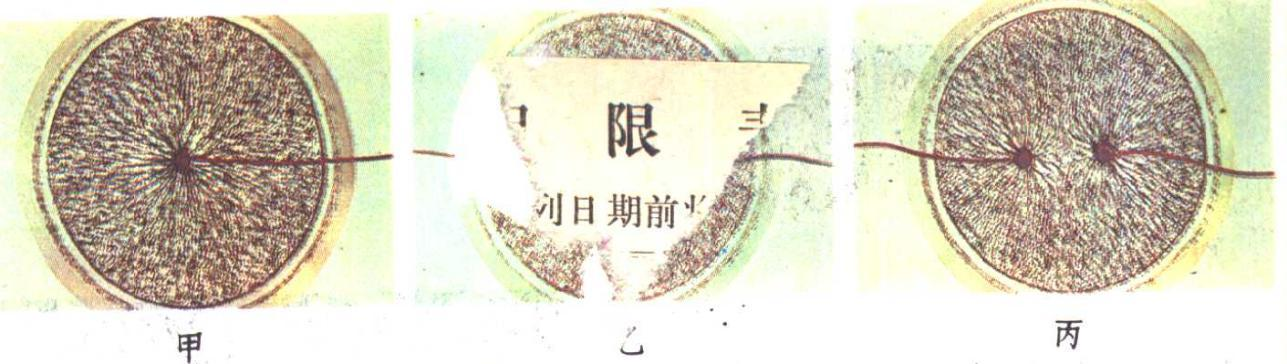
\includegraphics[max width=1.0\textwidth]{images/01913056-1f15-74d8-9184-9aab52c9d66b_3_802007.jpg}
\end{center}

图 1 点电荷的电场

\begin{center}
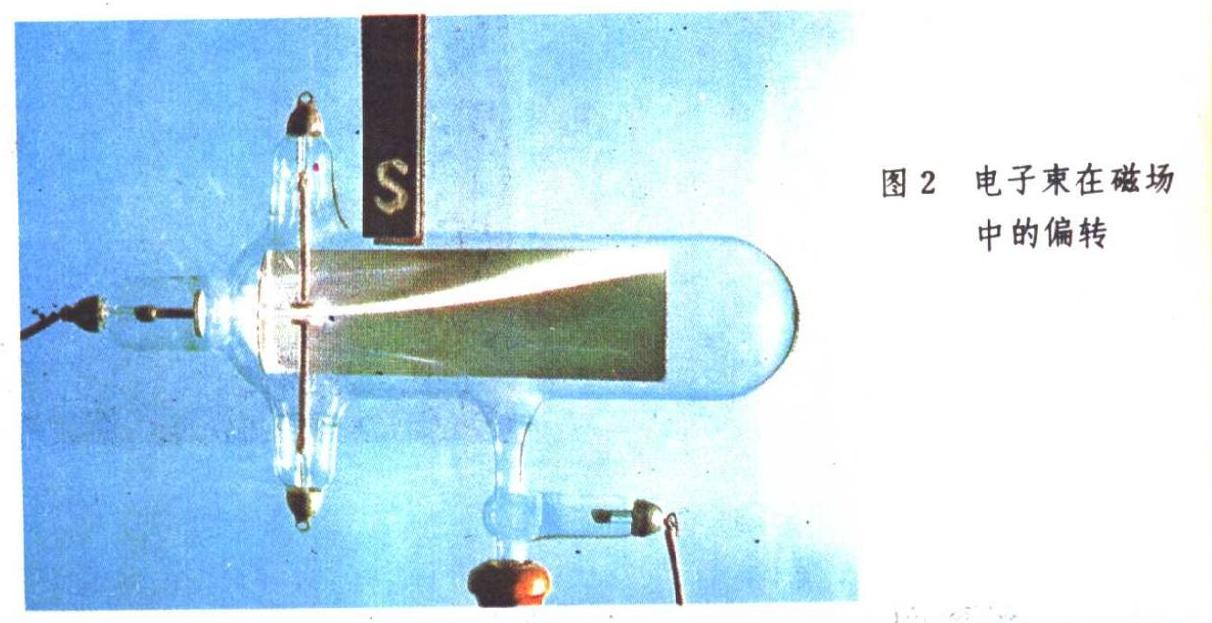
\includegraphics[max width=1.0\textwidth]{images/01913056-1f15-74d8-9184-9aab52c9d66b_3_778936.jpg}
\end{center}

图 3 我国发射的第一颗

通信卫星

\begin{center}
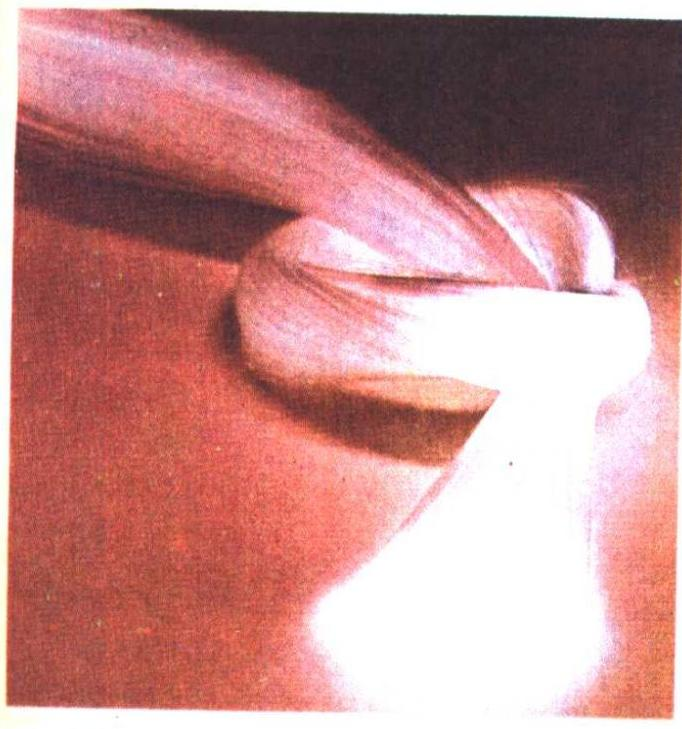
\includegraphics[max width=0.7\textwidth]{images/01913056-1f15-74d8-9184-9aab52c9d66b_4_564823.jpg}
\end{center}

4 图 4 光导纤维

\begin{center}
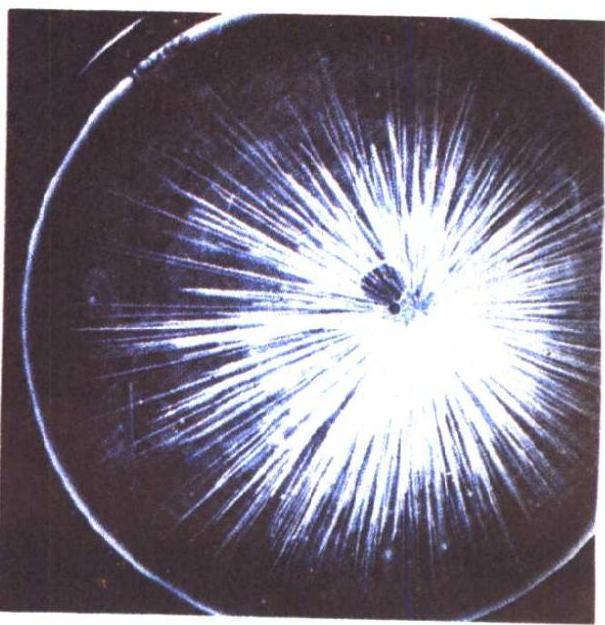
\includegraphics[max width=0.6\textwidth]{images/01913056-1f15-74d8-9184-9aab52c9d66b_4_181375.jpg}
\end{center}

图 5 云室中 \(\alpha\) 粒子的径迹

\begin{center}
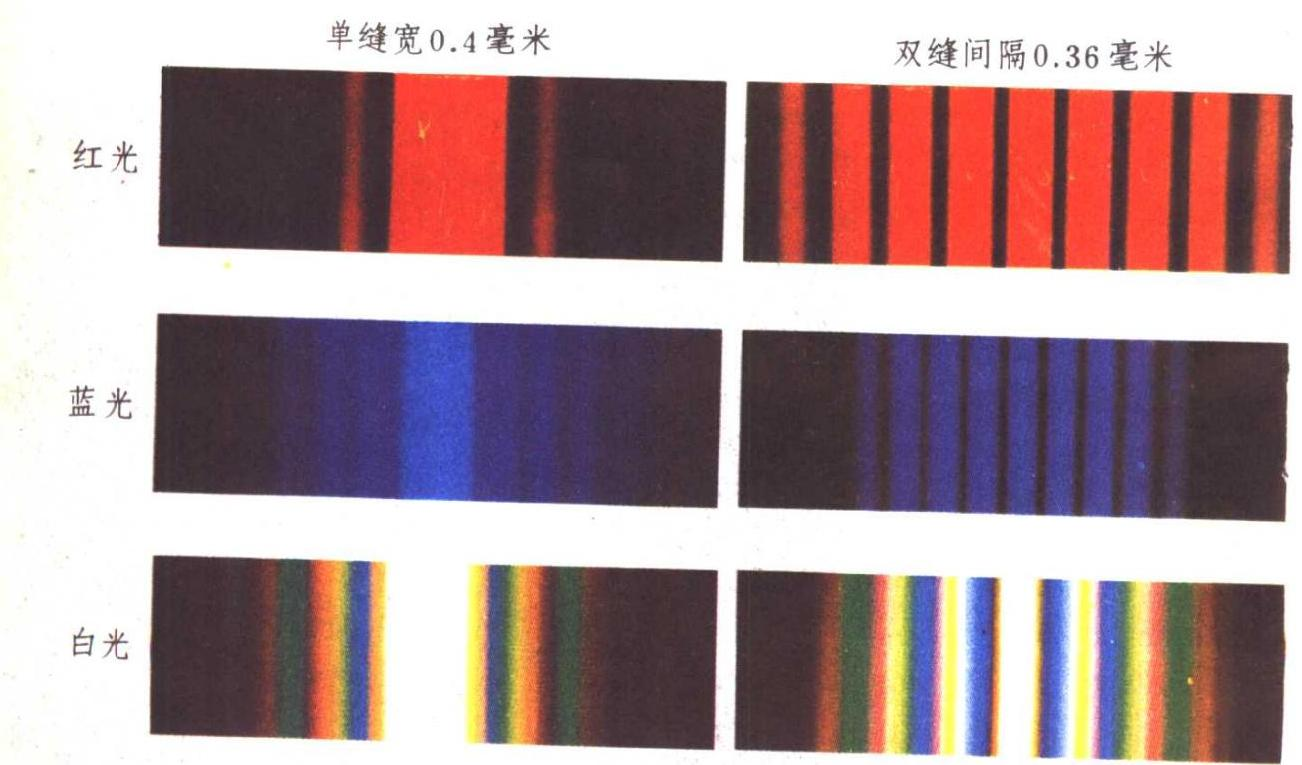
\includegraphics[max width=1.0\textwidth]{images/01913056-1f15-74d8-9184-9aab52c9d66b_4_537717.jpg}
\end{center}

图 6 干涉和衍射条纹

\begin{center}
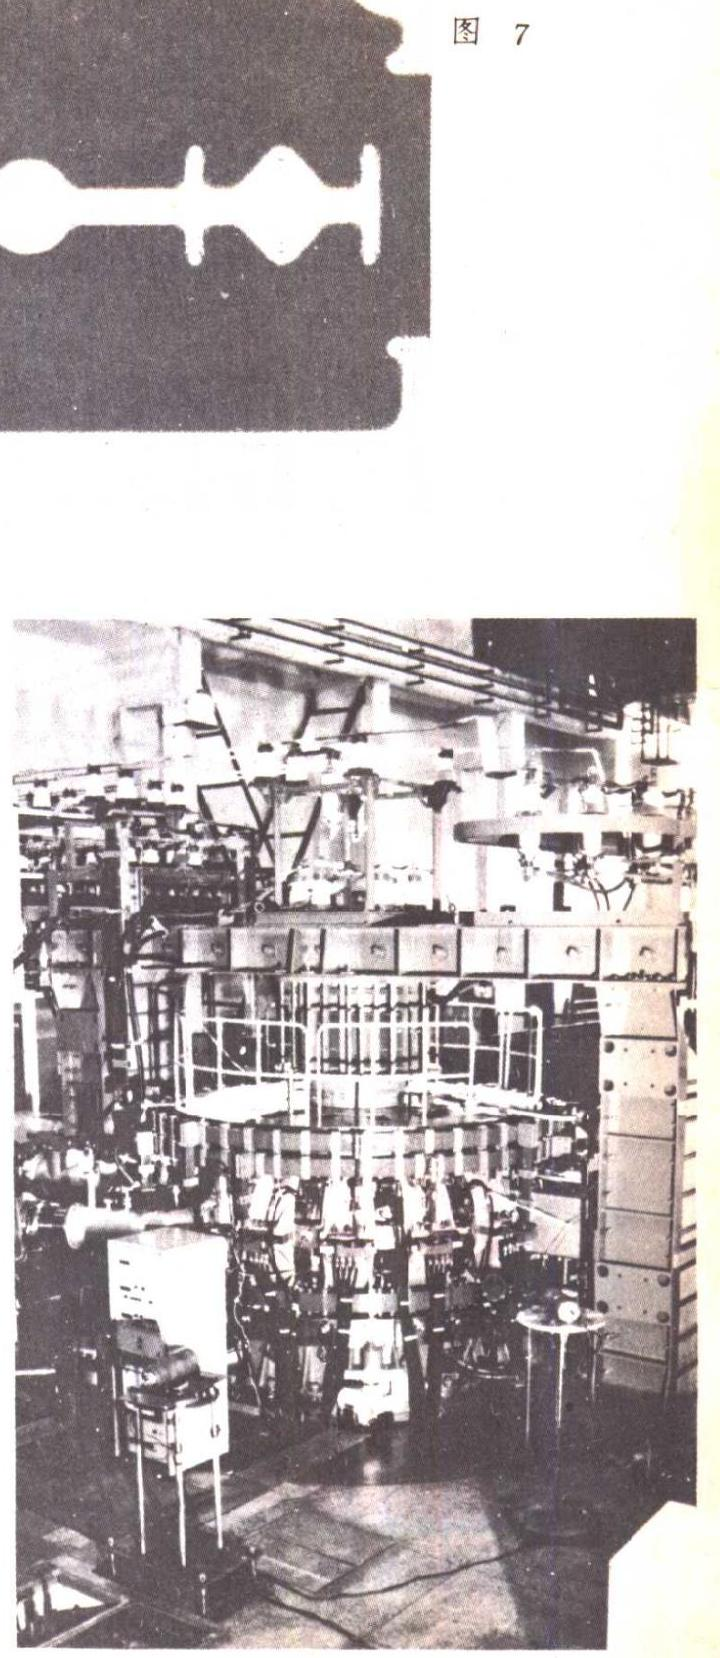
\includegraphics[max width=0.8\textwidth]{images/01913056-1f15-74d8-9184-9aab52c9d66b_5_406445.jpg}
\end{center}

图 9 “中国环流器一号” 主机

\begin{center}
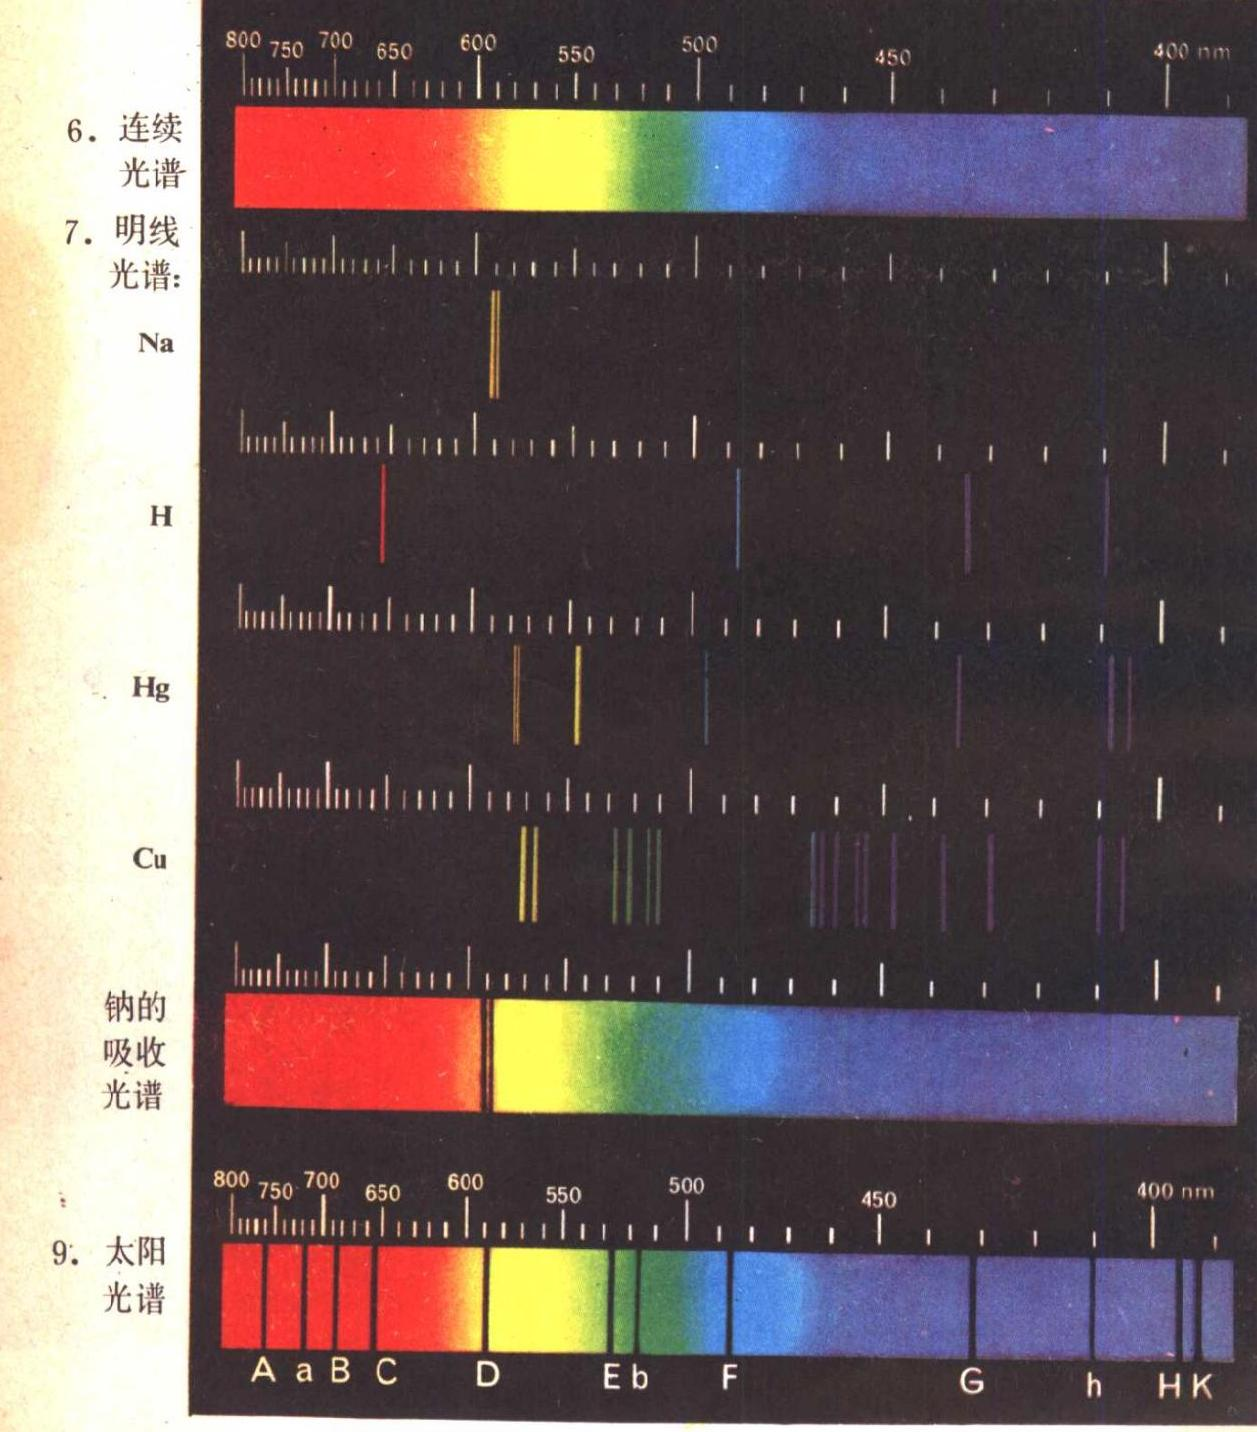
\includegraphics[max width=1.0\textwidth]{images/01913056-1f15-74d8-9184-9aab52c9d66b_6_164842.jpg}
\end{center}

图 10

\section*{说 明}

这册课本是根据教育部颁发的《高中物理教学纲要(草案)》基本要求内容, 参考《全日制十年制学校高中课本 (试用本) 物理下册》编写的. 许多省、市、自治区的教师, 在本书编写过程中给予了大力支持, 在此谨致谢意.

\section*{目 录}

第一章 电场 .1

一、库仑定律 \(\cdot 2\)

二、电场 电场强度 \(\cdots 7\)

三、电力线 \(\cdot {10}\)

四、电场中的导体 -13

五、电势能 电势差 .16

六、电势 等势面 19

七、电势差跟电场强度的关系 -22

人、带电粒子在匀强电场中的运动 -24

九、示波管 .28

十、电容器 电容 -31

十一、平行板电容器的电容 常用电容器 -33

十二、电容器的连接* .36

十三、静电的防止和应用 -38

第二章 稳恒电流 -47

一、电流 47

二、欧姆定律 .49

三、电阻定律 -53

四、电功和电功率 -56

五、焦耳定律 -58

六、串联电路 .60

七、并联电路 .64

八、分压和分流在伏特表和安培表中的应用 .69

九、电动势 .73

十、闭合电路的欧姆定律 -75

十一、电池组 .79

十二、电阻的测量 -83

第三章 磁场 - 91

一、磁场 -.91

二、磁现象的电本质 磁性材料 .95

三、磁感应强度 .98

四、磁场对电流的作用 102

五、电流表的工作原理 105

六、磁场对运动电荷的作用 106

七、带电粒子的圆周运动 108

八、回旋加速器* .112

第四章 电磁感应. 121

一、电磁感应现象 . 121

二、感生电流的方向 楞次定律 126

三、法拉第电磁感应定律 -130

四、自感 136

五、涡流* -140

第五章 交流电 .147

一、交流电的产生 -147

二、表征交流电的物理量 -152

三、纯电感电路 - 154

四、纯电容电路 - 158

五、三相交流电 - 161

六、感应电动机 -164

七、变压器 - 168

八、远距离输电 - 173

第六章 电磁振荡和电磁波. 181

一、电磁振荡 -181

二、电磁振荡的周期和频率 -184

三、电磁场和电磁波 186

四、电磁波的发射 190

五、电磁波的接收 193

六、电磁波的传播特性* 196

七、传真 电视 雷达* .200

八、我国广播电视事业的发展 .205

第七章 电子技术初步知识 .209

一、二极管及其单向导电性 .209

二、整流和滤波电路* .212

三、三极管及其放大作用 -218

四、晶体管放大器* .221

五、简单收音机的原理 .225

六、电子技术的发展及其对科学技术的影响 .226

第八章 光的反射和折射. .231

一、光的直线传播 .231

二、光的速度 .235

三、光的反射 平面镜 .238

四、球面镜 \(\cdot {242}\)

五、光的折射 .2.45

六、全反射 .251

七、棱镜 -258

八、透镜 -262

九、透镜成像作图法 .265

十、透镜公式 -270

十一、眼睛 .273

十二、显微镜和望远镜 -277

第九章 光的本性. .285

一、光的微粒说和波动说 .285

二、双缝干涉 -287

三、薄膜干涉 -291

四、光的衍射 2,294

五、光的电磁说 电磁波谱 -297

六、光谱和光谱分析 -301

七、光电效应 : 303

八、光的波粒二象性 .310

第十章 原子和原子核. -315

一、原子的核式结构的发现 -315

二、玻尔的原子模型 -319

三、玻尔理论的成功和局限 .322

四、天然放射现象 -328

五、探测放射线的方法* .333

六、原子模的人工转变 原子核的组成 -336

七、放射性阈位素 -340

八、核能 -343

丸、重核的裂变 -346

十、轻核的聚变 -351

学生实验 -358

一、电场中等势线的描绘 -358

二、练习使用示波器* -359

三、测定金属的电阻率 .363

四、把电流表改装为伏特表 -365

五、用安培表和伏特表测定电池的电动势和内电阻 -366

六、练习使用万用电表测电阻 -368

七、观察磁铁对电流的作用* .370

八、研究电磁感应现象 .372

九、用示波器观察交流电的波形* -373

十、用示波器观察交流电的整流和滤波* .376

十一、安装简单的收音机* .378

十二、测定玻璃的折射率 3.379

十三、测量凸透镜的焦距 -380

十四、观察双缝干涉现象* -381

十五、用卡尺观察光的衍射现象 -382

附录一 常用的电磁学量的国际制单位 -384

附录二 常用的物理恒量. .385

\section*{第一章 电 场}

人类很早就认识了磁现象和电现象. 例如, 我国在战国末期就发现了磁铁矿吸引铁的现象, 在东汉初年就有带电的琥珀吸引轻小物体的文字记载. 但是, 人类对电磁现象的系统研究却是在欧洲文艺复兴之后才逐渐开展起来的, 到十九世纪才建立了完整的电磁学理论.

电磁学及其应用对人类的影响十分巨大. 在电磁学研究基础上发展起来的电能的生产和利用, 是历史上的一次技术革命, 是人类改造世界能力的飞跃, 打开了电气化时代的大门.

目前, 世界面临一次新的技术革命, 出现了微电子技术、 电子计算机、光纤通讯、生物技术、新能源、新材料、空间技术、 海洋开发等一批新技术. 它们的共同特点是知识高度密集, 即需要集中大量科学技术人才, 工人的劳动也不是主要靠体力, 而要靠智力和知识. 在这些新技术中, 起带头作用的是在电磁学研究基础上发展起来的微电子技术和电子计算机. 它们被广泛应用于各种新技术领域, 带动这些技术迅猛发展, 而且越来越深地渗透到化工、冶金、机器制造等传统技术领域中, 引起这些领域的深刻变革.

让我们努力学好电磁学知识, 为迎接新的技术革命、为实现社会主义祖国的现代化, 作好准备吧!

\section*{一、库仑定律}

两种电荷 我们已经知道自然界的电荷只有两种, 即正电荷和负电荷. 用绸子摩擦过的玻璃棒所带的电荷是正电荷; 用毛皮摩擦过的硬橡胶棒所带的电荷是负电荷. 电荷之间有相互作用, 同种电荷互相排斥, 异种电荷互相吸引. 但是, 电荷间作用力的大小跟什么有关系呢? 下面我们通过实验来研究这个问题.

库仑定律 先把一个带正电的物体放在 \(A\) 处,然后把一个挂在丝线下端的带正电的小球,先后挂在 \({P}_{1}\text{、}{P}_{2}\cdots \cdots {P}_{8}\) 等位置 (图 1-1). 带电小球受到电力的大小, 可以通过丝线

\begin{center}
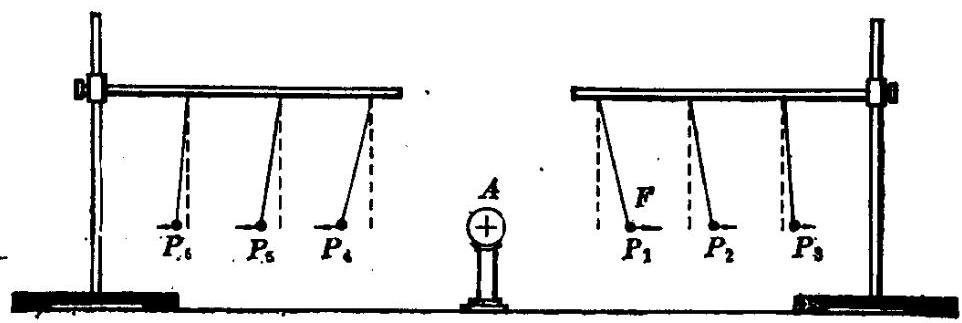
\includegraphics[max width=1.0\textwidth]{images/01913056-1f15-74d8-9184-9aab52c9d66b_14_359528.jpg}
\end{center}

图 1-1

对竖直方向的偏角大小显示出来. 实验表明,带电小球在 \({P}_{1}\) 、 \({P}_{2}\text{、}{P}_{3}\) 各点受到的电力依次减小; 在 \({P}_{4}\text{、}{P}_{5}\text{、}{P}_{6}\) 各点受到的电力也依次减小. 所以, 电荷之间的作用力随着距离的增大而减小.

增大丝线下端带电小球的电量, 在同一个位置, 小球受到的电力也增大. 所以, 电荷之间的作用力随着电量的增大而增大.

法国物理学家库仑 \(\left( {{1736} \sim {1806}}\right)\) ,用精确的实验研究了静止的点电荷间的相互作用力, 于 1785 年发现了后来用他的名字命名的定律.

真正的点电荷是不存在的, 但是, 如果带电体间的距离比它们的大小大得多, 以致带电体的形状和大小对相互作用力的影响可以忽略不计时, 这样的带电体就可以看成是点电荷. 点电荷是一种理想化的模型.

库仑实验的结果是: 在真空中两个点电荷间的作用力服它们的电量的乘积成正比, 跟它们间的距离的平方成反比, 作用力的方向在它们的连线上. 这就是库仑定律. 电荷间的这种作用力叫做静电力, 又叫做库仑力.

如用 \({Q}_{1}\text{、}{Q}_{2}\) 表示两个点电荷的电量,用 \(r\) 表示它们间的距离,用 \(F\) 表示它们间的静电力,库仑定律就可以写成下面的公式:

\[
F = k\frac{{Q}_{1}{Q}_{2}}{{r}^{2}}
\]

式中 \(k\) 是比例恒量,叫做静电力恒量.

在国际单位制中, 电量的单位就是我们在初中学过的库仑,简称库,国际符号是 \(\mathrm{C}\) . 如果上面公式中的物理量都用国际单位制的单位, 即力的单位用牛, 距离的单位用米, 电量的单位用库,由实验得出 \(k = 9 \times {10}^{9}\) 牛. 米 \({}^{2}/{\text{库}}^{2}\) .

很容易看出, 库仑定律和万有引力定律很相似, 它们都是平方反比律. 人们现在还不能说明为什么这两个定律如此相似, 但这种相似使我们可以用力学的比喻来理解许多电学问题.

基本电荷 我们知道, 电子带有最小的负电荷, 质子带有最小的正电荷, 它们的电量的绝对值相等. 一个电子的电量

\[
e = - {1.60} \times {10}^{-{19}}\text{库.}
\]

所有的实验还指出, 任何带电的粒子, 所带电量或者等于电子或质子的电量,或者是它们的电量的整数倍 \({}^{\left( 1\right) }\) . 因此,人们自然地把 \({1.60} \times {10}^{-{19}}\) 库叫做基 本电荷. 科学家 在研 究原子、 原子核以及基本粒子中, 为了方便, 常常用基本电荷作为电量的单位.

[例题] 在真空中有两个相距 0.3 米的点电荷, 带的电量分别是 \(+ 1 \times {10}^{-8}\) 库和 \(- 2 \times {10}^{-8}\) 库. 求两个电荷间的静电力.

在题日中,用 “+” “一” 号来表示电荷的正负. 但是在应用库仑定律求电荷间的相互作用力的大小时, 只用它们的绝对值进行计算就可以了.

解: \(F = k\frac{{Q}_{1}{Q}_{2}}{{r}^{2}} = \frac{9 \times {10}^{9} \times {10}^{-8} \times 2 \times {10}^{-8}}{{0.3}^{2}}\) 牛

\[
= 2 \times {10}^{-5}\text{牛.}
\]

由于两个电荷是异种的, 所以它们间的静电力是引力.

① 六十年代以来, 在高能物理的研究中提出了一个设想, 认为质子, 中子等粒子是由更基本的层子 (或夸克) 组成的, 层子所带电量是基本电荷的 \(1/3\) 或 \(2/3\) . 但是,人们一直还没有在实验中观察到层子.

\section*{阅读材料: 库仑扭秤实验}

库仑定律是通过扭秤实验发现的. 扭秤的主要部分是在一根细金属丝下面悬挂一根玻璃棒, 棒的一端有一个金属小球 \(A\) ,另一端有一个平衡小球 \(B\) . 在离 \(A\) 球某一距离的地方. 再放一个跟 \(A\) 球相同的金属小球 \(C,C\) 被固定在扭秤盖上 (图 1-2). 如果 \(A\) 球和 \(C\) 球带同种电荷,它们间的斥力将使玻璃棒转过一个角度. 向相反方向扭转旋钮 \(M\) ,玻璃棒可以回到原来的位置并保持静止, 这时金属丝扭转弹力的力矩跟电荷间斥力的力矩平衡. 因此从旋钮 \(M\) 转过的角度可以计算出电荷间作用力的大小.

\begin{center}
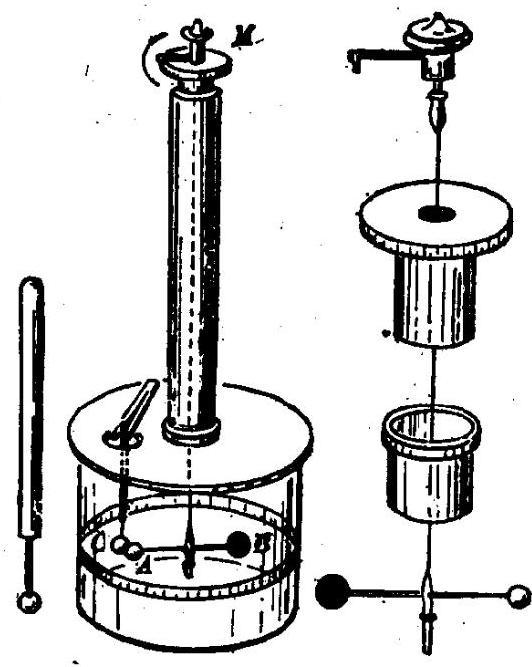
\includegraphics[max width=0.6\textwidth]{images/01913056-1f15-74d8-9184-9aab52c9d66b_17_396112.jpg}
\end{center}

图 1-2 库仑扭秤

库仑早就推测电荷之间的作用力跟它们之间的距离的平方成反比. 库仑利用扭秤在 \(A\text{、}C\) 两球电量不变的情况下,测量了两个小球在不同距离下的力, 发现这个力确实跟距离的平方成反比, 从而证实了自己的推测.

在库仑做扭秤实验的时候, 还不知道怎么来测量电量, 电量的单位也还没有确定. 库仑用一个简单的办法巧妙地解决了这个困难. 他为了改变带电小球的电量, 就将这个带电小球跟与它同样的但不带电的金属小球相碰, 由于两个小球完全相同, 它们带的电量也一定相等, 从而使带电小球的电量减小到原来的 \(\frac{1}{2}\) (图 1-3). 再用同 样的方法可以使带电小球的电量减小到原来的 \(\frac{1}{4}\) 、 \(\frac{1}{8}\) 等等. 库仑用这种方法来改变带电小球的电量, 但保持两球之间的距离不变, 利用扭秤测量了带电小球之间的作用力, 发现作用力跟它们所带电量的乘积成正比.

\begin{center}
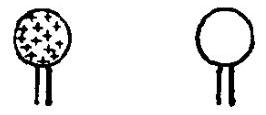
\includegraphics[max width=0.3\textwidth]{images/01913056-1f15-74d8-9184-9aab52c9d66b_18_594411.jpg}
\end{center}

\begin{center}
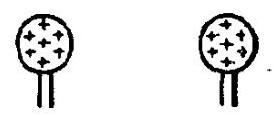
\includegraphics[max width=0.3\textwidth]{images/01913056-1f15-74d8-9184-9aab52c9d66b_18_498094.jpg}
\end{center}

图 1-3

\section*{练 习 -}

(1)通过什么事实可以证明自然界中只有两种电荷? (参看初中物理第二册 \({118} \sim {119}\) 页).

(2). 真空中的两个点电荷,带的电量分别是 \(+ {4.0} \times {10}^{-9}\) 库和 \(- {2.0} \times {10}^{-9}\) 库,相距 10 厘米. 每个电荷受到的静电力有多大, 是引力还是斥力?

(3)原子核的半径大约为 \({10}^{-{14}}\) 米,假定核中两个质子相距这么远, 其间的静电力大约有多大?

(4)在真空中, 两个点电荷之间的距离为 1.0 米时, 相互排斥的力为 \({1.0} \times {10}^{-3}\) 牛. 当它们相距 10 厘米时,相互排斥的力将是多大?

\section*{二、电场 电场强度}

电场 任何力的作用都离不开物质. 手推桌子, 手对桌子的推力直接作用在桌子上. 马拉车, 马对车的拉力是通过绳子作媒介. 两个电荷相互作用时并不直接接触, 它们之间的相互作用也是通过别的物质作媒介而发生的, 这种物质就是电场.

只要有电荷存在,在电荷的周围就存在着电场, \(A\text{、}B\) 两个电荷相互作用时, \(A\) 电荷受到的 \(B\) 电荷的作用,实际上是 \(B\) 电荷的电场对 \(A\) 电荷的作用. 同样, \(B\) 电荷受到的 \(A\) 电荷的作用,实际上是 \(A\) 电荷的电场对 \(B\) 电荷的作用.

电场强度 电场的最基本的特性是它对放入其中的电荷发生力的作用. 我们研究电场, 希望知道任意电荷在电场中任意一点受到的电场力.

\begin{center}
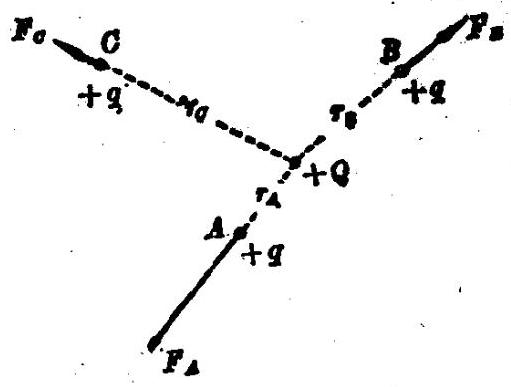
\includegraphics[max width=0.5\textwidth]{images/01913056-1f15-74d8-9184-9aab52c9d66b_19_780794.jpg}
\end{center}

图 1-4

假设在真空中有一个由正电荷 \(Q\) 产生的电场 (图 1-4). 我们把另一个正电荷 \(q\) 放在距 \(Q\) 为 \({r}_{A}\) 的 \(A\) 点. \(q\) 受到的电场力 \({F}_{A} = k\frac{Qq}{{r}_{A}^{2}} = q\left( \frac{kQ}{{r}_{A}^{2}}\right)\) . 比值 \(\frac{{F}_{A}}{q}\) 等于单位电荷在 \(A\) 点受到的电场力,知道了它就可以知道任意电荷在 \(A\) 点受到的电场力.

同样的道理,比值 \(\frac{{F}_{B}}{q}\text{、}\frac{{F}_{C}}{q}\) 分别等于单位电荷在 \(B\) 点、 \(C\) 点受到的电场力,知道了它们就可以知道任意电荷在 \(B\) 点、 \(C\) 点受到的电场力.

放入电场中某一点的电荷受到的电场力跟它的电量的比值, 叫做这一点的电场强度, 简称为场强. 某一点的场强越大, 单位电荷在该点受到的电场力就越大.

如果用 \(E\) 表示电场强度,用 \(F\) 表示电荷 \(q\) 受到的电场力, 那么,

\[
E = \frac{F}{q}. \tag{1}
\]

场强跟力一样, 也是矢量. 我们规定电场中某点的场强方向跟正电荷在该点的受力方向相同.

电场强度的单位是牛/库. 电场中的某一点, 如果 1 库的电荷在该点受到的电场力是 1 牛, 这点的场强就是 1 牛/库.

从上面讲的很容易知道,在点电荷 \(Q\) 的电场中,在距离 \(Q\) 为 \(r\) 的 \(P\) 点,场强 \(E\) 的大小为

\[
E = \frac{kQ}{{r}^{2}} \tag{2}
\]

\begin{center}
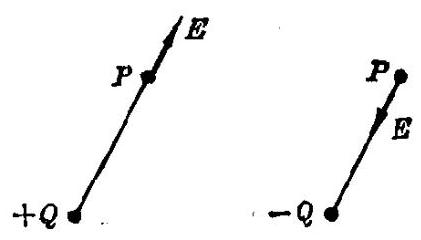
\includegraphics[max width=0.4\textwidth]{images/01913056-1f15-74d8-9184-9aab52c9d66b_20_883197.jpg}
\end{center}

图 1-5 场强的方向

如果 \(Q\) 是正电荷, \(E\) 的方向就是沿着 \({QP}\) 连线并离 \(Q\) 而去,如果 \(Q\) 是负电荷, \(E\) 的方向就是沿着 \({QP}\) 连线并向 \(Q\) 而来 (图 1-5).

应该注意, (1) 式和 (2) 式虽然都表示电场中某点的场强, 但它们的意义是不同的. (1) 式是场强的定义式, 对任何电场都是适用的. (2) 式是点电荷在真空中的电场中场强的计算式, 只适用于点电荷在真空中的电场.

如果有几个点电荷同时存在, 它们的电场就互相叠加, 形成合电场. 这时某点的场强, 就等于各个点电荷在该点产生的场强的矢量和. 例如图 1-6 中, \(P\) 点的场强 \(E\) 就等于 \({Q}_{1}\) 在该点产生的场强 \({E}_{1}\) 和 \({Q}_{2}\) 在该点产生的场强 \({E}_{2}\) 的矢量和.

\begin{center}
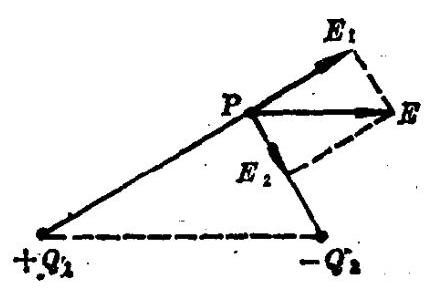
\includegraphics[max width=0.4\textwidth]{images/01913056-1f15-74d8-9184-9aab52c9d66b_21_278916.jpg}
\end{center}

图 1-6

\section*{练习 二}

(1)请你判断下面一些说法的对错.

① 根据公式 \(E = \frac{F}{q}\) ,可知电场强度跟电场力成正比,跟放入电场中的电荷的电量成反比.

② 电场强度的方向总是跟电场力的方向一致.

③ 用负电荷受到的电场力跟它的电量的比值也可以求出电场强度的大小, 不过电场强度的方向跟负电荷受到的电场力的方向相反.

(2)在真空中,有一个点电荷 \(Q\) ,它的电量是 \(- {6.6} \times {10}^{-9}\) 库,求离它 10 厘米的 \(A\) 点的电场强度.

(3)在真空中,离点电荷 \(Q\) 的距离是 5.0 厘米远的 \(A\) 点的场强是 \({3.0} \times {10}^{5}\) 牛/库, \(Q\) 带的电量是多少?

(4)真空中有一个电场, 在这个电场中的某一点放入电量为 \({5.0} \times {10}^{-9}\) 库的点电荷,它受到的电场力为 \({3.0} \times {10}^{-4}\) 牛, 求这一点处的电场强度是多大:

(5)在氢原子中,电子和质子的平均距离是 \({0.53} \times {10}^{-{10}}\) 米. 质子在这个距离处产生的场强是多大? 方向如何? 电子受到的力是多大? 方向如何?

\section*{三、电 力 线}

电力线 如果能够用图形把电场中各点场强的大小和方向形象地表示出来, 这对我们认识电场是很有好处的. 在图 1-7 里回出的正电荷和负电荷的电场中的一些矢量, 能表示出场内各点的场强的大小和方向. 但是, 更好的办法是用英国物理学家法拉第 \(\left( {{1791} \sim {1867}}\right)\) 引入的电力线来形象地表示电场.

\begin{center}
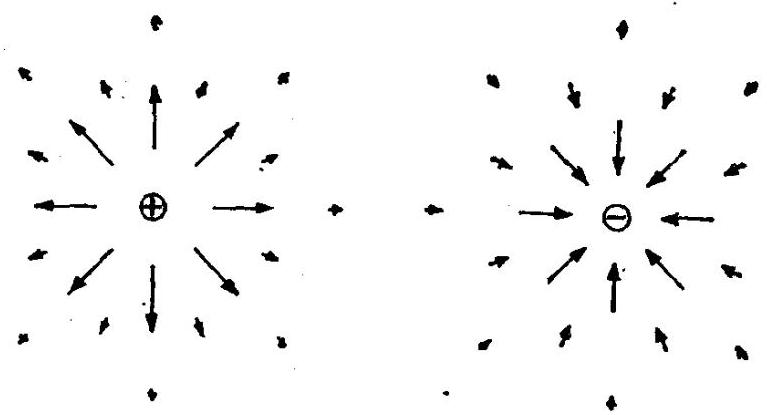
\includegraphics[max width=0.8\textwidth]{images/01913056-1f15-74d8-9184-9aab52c9d66b_22_112557.jpg}
\end{center}

图 1-7

在任何电场中,每一点的场强 \(E\) 都有一定的方向,所以我们可以在电场中画出一系列的从正电荷出发到负电荷终止的曲线, 使曲线上每一点的切线方向都跟该点的场强方向一

\begin{center}
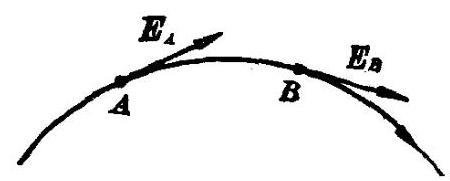
\includegraphics[max width=0.5\textwidth]{images/01913056-1f15-74d8-9184-9aab52c9d66b_22_264528.jpg}
\end{center}

图 1-8

致, 这些曲线就叫做电力线. 图 1-8 是一条电力线, 它上面的 \(A\text{、}B\) 点上的场强 \({E}_{A}\text{、}{E}_{B}\) 在各该点的切线上,方向如图 中箭头所示.

电力线的形状可以用实验来模拟, 把奎宁的针状结晶或头发屑悬浮在蓖麻油里, 再放入电场中, 就可以看到微屑按照场强的方向排列起来 (见插页图 1), 形成电力线. 应该注意, 虽然我们可以用实验来模拟电力线, 但电力线并不是电场里实际存在的线, 而是人们为了使电场形象化而假想的线.

图 1-9 是点电荷的电力线, 图 1-10 是两个等量的电荷的电力线. 从图 中可以看出, 在离产生电场的电荷较近 的地方, 也就是场强越大的地方, 电力线越密. 所以, 用电力线来表示电场时, 场强越大的地方电力线越密, 场强越小的地方电力线越稀.

\begin{center}
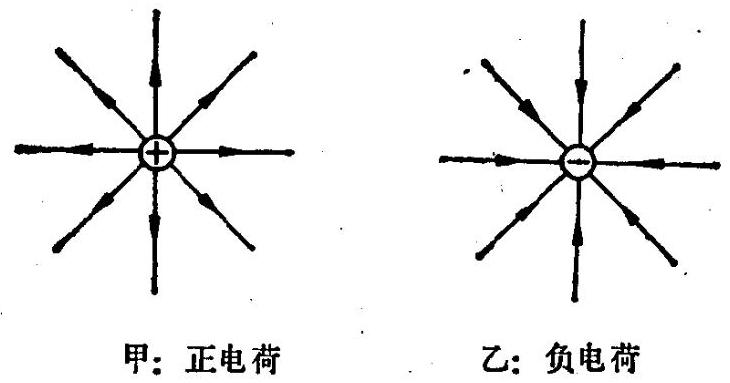
\includegraphics[max width=0.8\textwidth]{images/01913056-1f15-74d8-9184-9aab52c9d66b_23_315782.jpg}
\end{center}

图 1-9

\begin{center}
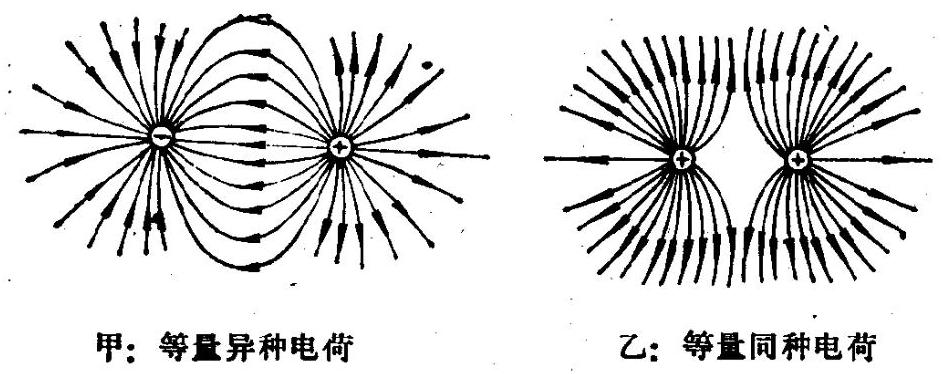
\includegraphics[max width=1.0\textwidth]{images/01913056-1f15-74d8-9184-9aab52c9d66b_23_298368.jpg}
\end{center}

图 1-10

匀强电场 在电场的某一区域里, 如果各点的场强的大小和方向都相同, 这个区域的电场就叫做匀强电场. 匀强电场是最简单的同时也是很重要的电场.

在匀强电场里, 既然各点的场强的方向都相同, 电力线就一定是互相平行的直线; 既然各点的场强的大小都相同, 电力线的疏密程度也一定处处相等. 因此, 匀强电场中的电力线, 是距离相等的互相平行的直线.

\begin{center}
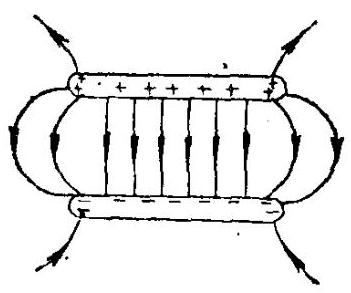
\includegraphics[max width=0.4\textwidth]{images/01913056-1f15-74d8-9184-9aab52c9d66b_24_754090.jpg}
\end{center}

图 1-11 匀强电场

两块靠近的大小相等互相正对并且互相平行的金 属板, 在分别带等量的正电和负电的时候, 它们间的电场, 除边缘附近外, 就是匀强电场 (图 1-11).

\section*{练 习 三}

(1)有人说电力线就是带电粒子在电场中运动的轨迹. 这个说法对吗? 为什么?

(2)在图 1-9 和图 1-10 中, 所有的电力线都不相交. 我们能否断言, 电场中任何两条电力线都不相交. 为什么?

(3)有两块水平放置的带电金属板, 上板带正电, 下板带等量的负电. 板间有一个塑料小球悬浮不动. 塑料小球受到哪些方的作用? 这些力的方向如何? 塑料小球带的是正电还是负定?

\section*{四、电场中的导体}

静电感应 我们在初中学过, 导体的特征是在它的内部有大量的可以到处移动的自由电荷. 对于金属导体来说, 这种自由电荷就是自由电子. 一块金属, 它的中性原子的最外层电子跟原子核的联系很弱, 在其余原子的作用下脱离了原来的原子而在整块金属中“游荡”, 成为自由电子. 失去了外层电子的原子变成带正电的离子, 在平衡位置附近做热振动. 所以, 整块金属就是由做热振动的正离子和在它们之间做无规则的热运动的自由电子组成的.

把金属导体放进电场中, 导体内部的自由电子受到电场力的作用, 将向电场的反方向作定向移动 (图 1-12 甲), 结果会使导体的两端分别出现正、负电荷. 这种现象叫做静电感应.

\begin{center}
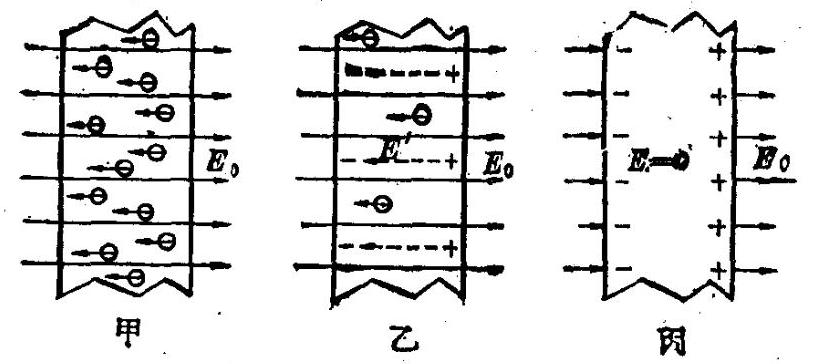
\includegraphics[max width=0.9\textwidth]{images/01913056-1f15-74d8-9184-9aab52c9d66b_25_314324.jpg}
\end{center}

图 1-12

由于静电感应而在导体两端出现的正、负电荷的电量是相等的. 这是因为自由电子定向移动到一端时, 另一端便剩有带电量跟电子相等的正离子.

导体内部的电场 把导体放进场强为 \({E}_{0}\) 的电场中时,由于静电感应出现的正、负电荷产生一个附加电场 \({E}^{\prime }\) (图 1-12 乙),跟外电场 \({E}_{0}\) 相叠加. 在导体内,附加电场 \({E}^{\prime }\) 跟外电场 \({E}_{0}\) 方向相反,叠加的结果削弱了导体内部的电场. 只要合场强 \(E\) 不等于零,导体内部就继续有电荷移动,两端的电荷要继续增加,使 \({E}^{\prime }\) 继续增大,直到合场强 \(E\) 等于零为止. 这时自由电荷的定向移动停止了 (图 1-12 丙), 我们就说导体处于静电平衡状态.

所以, 处于静电平衡状态的导体, 内部的场强必定处处为零.

从外部把电荷加给导体, 使它带电, 所加的电荷由于静电斥力, 彼此尽量远离, 因而分布在导体的外表面上, 导体内部没有净电荷.

处于静电平衡状态下的带电导体, 净电荷只分布在外表面上, 这个事实可以用下述的法拉第圆筒实验来验证. 如图 1-13所示,取两个验电器 \(A\) 和 \(B\) ,在 \(B\) 上装一个几乎封闭的空心金属圆筒 \(C\) (叫做法拉第圆筒). 使 \(B\) 和 \(C\) 带电, \(B\) 的箔片张开. 用有绝缘柄的金属小球 \(e\) 先跟 \(C\) 的外部接触,再把 \(e\) 移到 \(A\) 并跟 \(A\) 的金属球接触 (图 1-13 甲). 经过若干次以后,可以看到 \(A\) 的箔片张开,同时 \(B\) 的箔片张开的角度减小. 这表明 \(e\) 把 \(C\) 的一部分电荷搬运给了 \(A\) . 可见法拉第圆筒的表面是带有电荷的. 如果让 \(e\) 不接触 \(C\) 的表面,而是接触 \(C\) 的内部, 重做上述实验 (图 1-13 乙),不论重复多少次, \(A\) 的箔片都不张开, \(B\) 的箔片张开的角度也不减小. 这表明 \(e\) 并没有把 \(C\) 的电荷搬运给 \(A\) ,可见法拉第圆筒的内部不带电.

\begin{center}
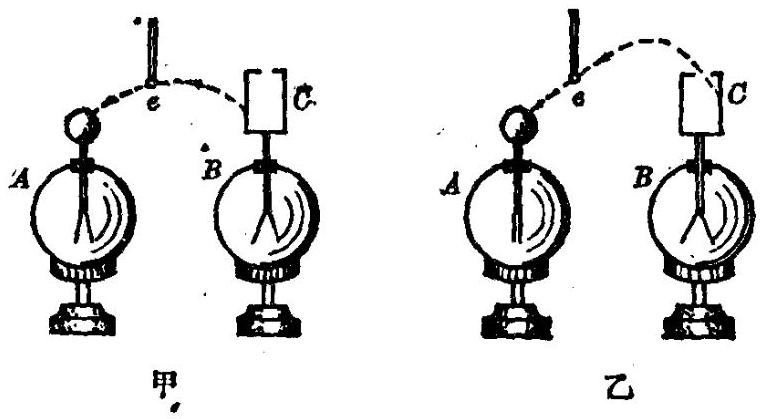
\includegraphics[max width=0.8\textwidth]{images/01913056-1f15-74d8-9184-9aab52c9d66b_26_839947.jpg}
\end{center}

图 1-13

静电屏蔽 静电平衡时导体内部的场强为零这一现象, 在技术上用来实现静电屏蔽.

如图 1-14 甲所示, 使带正电的金属球靠近验电器, 由于静电感应, 验电器的箔片要张开, 这表示验电器受到了附近的带电体的影响. 如果事先用一个金属网罩把验电器 罩住(图 1-14乙), 再让带电金属球靠近, 验电器的箔片就不张开了. 即使用导线把验电器和金属网罩连接上, 它的箔片也不张开. 可见, 金属网罩 (或金属包皮) 能把外电场遮住, 使内部不受外电场的影响, 这就是静电屏蔽.

\begin{center}
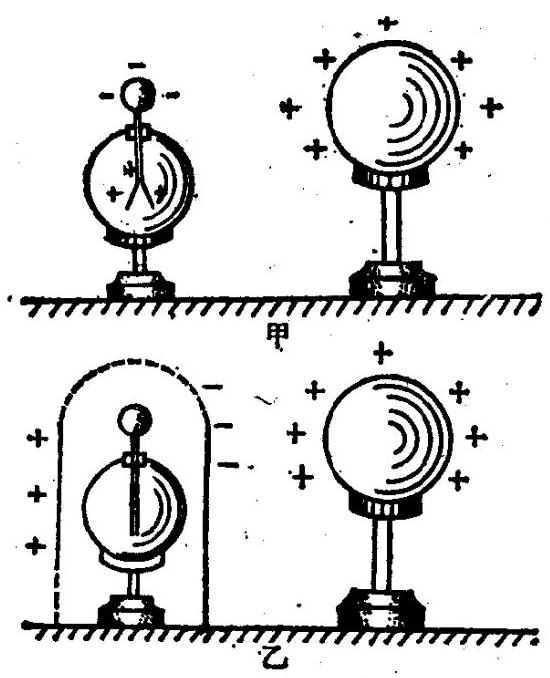
\includegraphics[max width=0.6\textwidth]{images/01913056-1f15-74d8-9184-9aab52c9d66b_27_599366.jpg}
\end{center}

图 1-14

有的电学仪器和电子设备的外面套有金属罩, 通讯电缆外面包一层铅皮, 都是用来防止外界电场的干扰, 起屏蔽作用的.

\section*{五、电势能 电势差}

电势能 地球上的物体受到重力的作用, 具有重力势能. 电场中的电荷受到电场力的作用, 也具有势能, 这种势能叫做电势能, 通常简称为电能.

\begin{center}
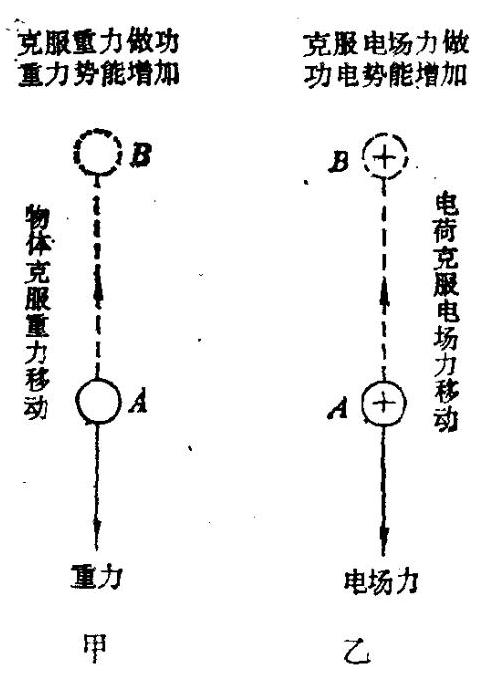
\includegraphics[max width=0.5\textwidth]{images/01913056-1f15-74d8-9184-9aab52c9d66b_28_549025.jpg}
\end{center}

图 1-15 重力势能和电势能

物体克服 重力从 \(A\) 点移动到 \(B\) 点 (图 1-15 甲),要克服重力做功. 克服重力做功的过程, 就是其他形式的能转化为重力势能的过程, 克服重力做了多少功, 物体就增加多少重力势能. 与此相似, 电荷克服电场力从 \(A\) 点移动到 \(B\) 点 (图 \({1}^{ * }\) \(- {15}\) ),要克服电场力做功. 克服电场力做功的过程, 就是其他形式的能转化为电势能的

过程, 克服电场力做了多少功, 电荷就增加多少电势能

正如重力做功使物体移动时物体 的重力势能减少一样, 电场力做功使电荷移动时电荷的电势能减少 (图 1-16). 电场力做了多少功, 电荷就减少多少电势能. 减少的电势能转化成电荷的动能或其他形式的能. 从图 1-16 可以看出, 正电荷

\begin{center}
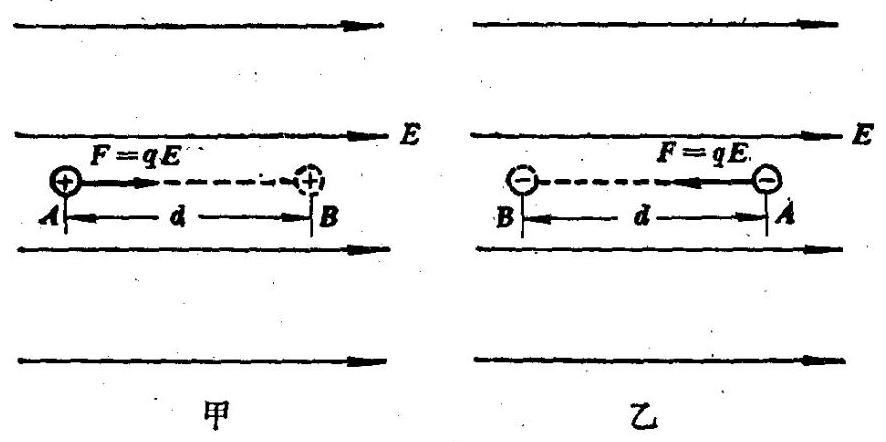
\includegraphics[max width=0.9\textwidth]{images/01913056-1f15-74d8-9184-9aab52c9d66b_29_484073.jpg}
\end{center}

图 1-16 电荷在电场力作用下移动时电势能减少

顺着电力线移动时电势能减少, 负电荷逆着电力线移动时电势能减少. 在匀强电场的情况下,减少的电势能 \(\Delta \mathcal{E} = W =\) \({qEd}\) .

电势差 研究电场常常需要知道任意电荷在电场中任意两点间移动时, 电势能的变化或需要做的功.

在图 1-16 所示的匀强电场中,电场力做功使 \(q\) 从 \(A\) 移到 \(B\) ,减少的电势能是 \(\Delta \mathcal{E} = W = {qEd}\) ; 克服电场力做功使 \(q\) 从 \(B\) 移到 \(A\) ,增加的电势能也是 \(\Delta \mathcal{E} = W = {qEd}\) . 比值 \(\frac{\Delta \mathcal{E}}{q}\) 等于在电场中 \(A\text{、}B\) 两点间移动单位电荷时电势能的改变量或需要做的功, 如果知道了这个比值, 就能求出在电场中两点间移动任意电荷时电势能的改变量和需要做的功.

电荷在电场中两点间移动时, 电势能的改变量跟电荷电

量的比值,叫做这两点间的电势差或电压. 如果用 \(\Delta \mathcal{E}\) 表示电荷 \(q\) 的电势能改变量,用 \(U\) 表示电势差,那么

\[
U = \frac{\Delta \mathcal{E}}{q}
\]

在国际单位制中, 电势差的单位是伏特, 简称伏, 国际符号是 V. 1 库电荷从一点移到另一点, 如果电势 能改变了 1 焦, 这两点间的电势差就是 1 伏.

如果知道了任意两点间的电势差, 就可以求出在这两点间移动电荷时电势能的变化和需要做的功, 而不必考虑电场力的大小和电荷移动的路径.

\[
\Delta \mathcal{E} = {qU};\;W = {qU}.
\]

\begin{center}
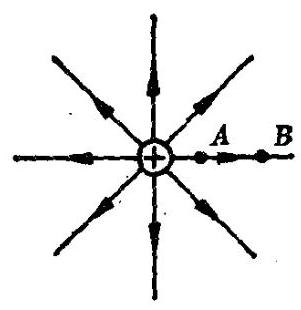
\includegraphics[max width=0.3\textwidth]{images/01913056-1f15-74d8-9184-9aab52c9d66b_30_144568.jpg}
\end{center}

图 1-17

〔例题] 图 1-17 表示一个正电荷的电场. 已知 \(A\text{、}B\) 间的电势差是 200 伏,有一电量为 \(- 6 \times {10}^{-8}\) 库的电荷从 \(B\) 移到 \(A\) ,它的电势能改变了多少? 是增加还是减少?

求电势能的改变量,可以将 \(U\) 和 \(q\) 的绝对值代入下式:

\[
\Delta \mathcal{E} = {qU} = 6 \times {10}^{-8} \times {200}\text{ 焦 } = {1.2} \times {10}^{-5}\text{ 焦. }
\]

电势能是增加还是减少了可以分三步来判定: (1)电场力是什么方向一由于移动的是负电荷, 它受到的电场力方向跟场强方向相反,由 \(B\) 指向 \(A\) ; (2) 电荷移动方向与电场力方向的关系一电荷由 \(B\) 向 \(A\) 移动,与受到的电场 力方向相同; (3) 是克服电场力做功还是电场力做功一是电场力做了功, 因而电势能减少. 所以, 本题的答案是电势能减少了 1.2 \(\times {10}^{-5}\) 焦.

\section*{练 习 四}

(1)把两个异种电荷间的距离增大一些, 是电场力做功还是外力克服电场力做功? 电势能是增加还是减少?

如果是把两个同种电荷间的距离增大一些呢?

(2)图 1-16 甲的电场中, \(A\) 点的电场强度方向如何? 如果在 \(A\) 点放一个负电荷,在电场力作用下它将向哪个方向移动? 它的电势能是增加还是减少?

(3)在图 1-16 乙的电场中,如果放一个正电荷,它在 \(A\) 、 \(B\) 两点的哪一点电势能较高? 为什么? 如果这个正电荷是 \(2 \times\) \({10}^{-8}\) 库,从 \(B\) 移到 \(A\) 电势能改变了 \(4 \times {10}^{-7}\) 焦, \(B\text{、}A\) 两点间的电势差是多少伏?

(4)在图 1-16 乙的电场中,如果 \(A\text{、}B\) 两点间的电势差是 30 伏,电量为 \(- 5 \times {10}^{-8}\) 库的电荷从 \(A\) 移到 \(\beta\) ,它的电势能怎样改变, 改变了多少?

\section*{六、电势 等势面}

电势 把电势能的改变量 \({qU}\) 和重力势能的改变量 \({mgh} =\) \({Gh}\) 相比较可以看出,电势差 \(U\) 跟高度差 \(h\) 相似.

我们常常不说高度差而说高度, 例如说室内吊灯的高度是 2.2 米. 这时我们是选定室内地 面作标 准位置 (认为它的高度是零), 把灯和地面的高度差作为灯的高度.

与此相似, 如果在电场中选一个标准位置, 那么电场中某点跟标准位置间的电势差, 就叫做该点的电势.

电势的单位和电势差的单位相同, 也是伏特. 被选作标准位置的电势等于零, 任何电荷在这个位置时的电势能也等于零.

单位正电荷在某点的电势能是几焦, 该点的电势就是几伏. 例如在图 1-18 所示的电场中,如果选定 \(C\) 点的电势为零,1 库正电荷在 \(A\) 点、 \(B\) 点的电势能分别为 10 焦、 4 焦, \(A\) 点、 \(B\) 点的电势就分别是 \({U}_{A} = {10}\) 伏、 \({U}_{B} = 4\) 伏; 当把 1 库正电荷由 \(A\) 或 \(B\) 移到 \(C\) 时,电场力要做 10 焦或 4 焦的功,使电势能减少到零.

\begin{center}
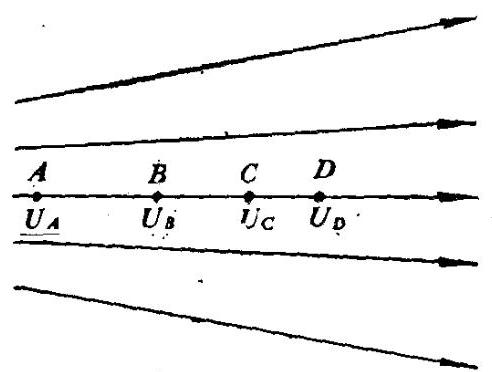
\includegraphics[max width=0.5\textwidth]{images/01913056-1f15-74d8-9184-9aab52c9d66b_32_878389.jpg}
\end{center}

图 1-18

在图 1-18 的电场中,单位正电荷从 \(D\) 移到零电势 \(C\) 时要克服电场力做功, 假定做的功是 3 焦, 电势能就增加了 3 焦而等于零,所以单位正电荷在 \(D\) 点的电势 能是 -3 焦,我们说 \(D\) 点的电势是 -3 伏.

电势差等于电势之差, 通常取绝对值. 例如图 1-18 中 \(D\text{、}A\) 两点的电势差 \({U}_{DA} = \left| {{U}_{D} - {U}_{A}}\right| = \left| {-3 - {10}}\right|\) 伏 \(= {13}\) 伏.

等势面 在地图上常用等高线来表示地形的高低, 与此相似, 在电场中常用等势面来表示电势的高低.

电场中电势相同的各点构成的面叫做等势面. 在同一等势面上任何两点间的电势差为零, 所以移动电荷时, 既不需要电场力做功, 也不需要克服电场力做功.

等势而一定跟电力线垂直, 即跟场强的方向垂直. 假如不是这样. 场强就有一个沿着等势面的分量, 这样在等势面上移动电荷时电场力就要做功. 但这是不可能的, 因为等势面上各点电势相等, 沿等势面移动电荷时电场力是不做功的. 所以, 场强一定跟等势面垂直.

沿着电力线方向移动正电荷, 电场力做功, 正电荷的电势能减小, 正电荷是从电势高的地方移向电势低的地方. 所以, 沿着电力线的方向电势越来越低. 可见, 电力线不但跟等势面垂直, 而且总是由电势较高的等势面指向电势较低的等势面.

匀强电场中的等势面是垂直于电力线的一族平面(图 1- 19), 点电荷的电场中的等势面是以点电荷为球心的一族球面 (图 1-20).

\begin{center}
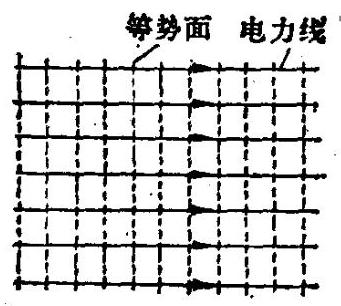
\includegraphics[max width=0.4\textwidth]{images/01913056-1f15-74d8-9184-9aab52c9d66b_33_753702.jpg}
\end{center}

图 1-19

\begin{center}
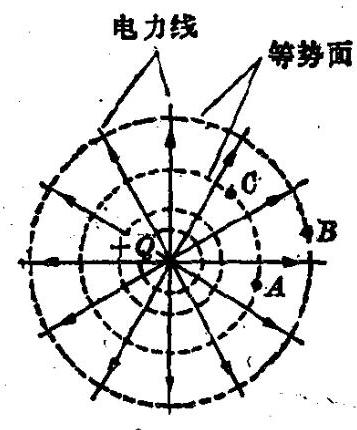
\includegraphics[max width=0.4\textwidth]{images/01913056-1f15-74d8-9184-9aab52c9d66b_33_823248.jpg}
\end{center}

图 1-20

处于静电平衡状态的导体, 内部的场强为零, 在任意两点间移动电荷都不需要做功, 所以任意两点间的电势差为零, 整个导体是个等势体, 导体表面是个等势面.

地球是个大导体, 在静电平衡状态的地球以及跟它相连的导体是等势体. 在实际工作中常常取地球或跟地球相连的导体作为标准位置, 认为它们的电势为零.

\section*{练 习 五}

(1) \(A\) 点的电势是 60 伏. 先后把电量分别是 \(3 \times {10}^{-8}\) 库和 \(2 \times {10}^{-9}\) 库的正电荷放在 \(\mathbf{A}\) 点,求它们的电势能.

(2)把一个电量为 \(5 \times {10}^{-8}\) 库的正电荷,从电势为零的 \(O\) 点移到电场内的 \(M\) 点,外力克服电场力做的功是 \({1.0} \times {10}^{-8}\) 焦, 求 \(M\) 点的电势. 如果把这个电荷从电场内的 \(N\) 点 移到 \(O\) 点, 电场力做的功是 \({2.0} \times {10}^{-6}\) 焦,求 \(N\) 点的电势.

(3)在图 1-18 中,如果选定 \(B\) 点的电势为零, \(D\text{、}A\) 两点的电势差是几伏? 如果选定 \(D\) 点的电势为零, \(D\text{、}A\) 两点的电势差是几伏? \(D\text{、}A\) 两点的电势差跟选哪点电势为零有没有关系?

(4)在图 1-16 的电场中, \(A\text{、}B\) 两点的电势相比,甲图中 \(\cdots \cdots\) 点的电势较高,乙图中......点的电势较高. 从图中可以看出, 在电场力作用下, 正电荷总是从电势较......的一点移向电势较......的一点; 负电荷总是从电势较......的一点移向电势较......的一点.

(5)把一个正电荷从图 1-20 的一个等势面上的 \(A\) 点移到另一个等势面上的 \(B\) 点,跟从 \(C\) 点移到 \(B\) 点电场力做的功相等吗?

\section*{七、电势差跟电场强度的关系}

电场中两点间电势差的大小跟电场强度是有关系的, 我们以匀强电场为例来研究这个关系.

设图 1-21 中 \(A\text{、}B\) 间的距离为 \(d\) ,电势差为 \(U\) ,场强为 \(E\) .

把正电荷 \(q\) 从 \(A\) 移到 \(B\) ,电场力做的功 \(W\) 可以表示为

\[
W = {qEd}\text{ 或 }W = {qU}\text{. }
\]

可见,

\[
U = {Ed}\text{.}
\]

\begin{center}
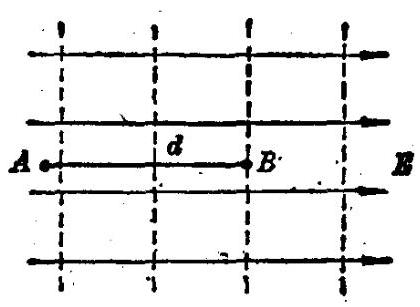
\includegraphics[max width=0.4\textwidth]{images/01913056-1f15-74d8-9184-9aab52c9d66b_35_473269.jpg}
\end{center}

图 1-21

这就是说, 在匀强电场中, 沿场强方向的两点间的电势差等于场强和两点间距离的乘积.

把上式改写成

\[
E = \frac{U}{d}
\]

这一等式说明, 在匀强电场中, 场强等于沿场强方向每单位长度上的电势差.

由上式可以得到场强的单位伏/米, 由于

\[
1\frac{\text{ 伏 }}{\text{ 米 }} = 1\frac{\text{ 焦 }}{\text{ 米 }} = 1\frac{\text{ 牛 } \cdot \text{ 米 }}{\text{ 库 } \cdot \text{ 米 }} = 1\frac{\text{ 牛 }}{\text{ 库 }},
\]

所以伏/米和牛/库这两个场强单位是相等的.

电势差跟电场强度的关系在实用上很重要. 这是因为没有测量电场强度的专门仪器, 但是有测量电势差的专门仪器 (参看第十一节), 根据测得的电势差, 利用电场强度跟电势差的关系, 可以算出电场强度的数值.

〔例题] 图 1-22 中, 金属圆板 \(A\text{、}B\) 相距 3 厘米. 用电压为 60 伏的电池组使它们带电后, 它们间的匀强电场的场强是多大, 方向如何?

\begin{center}
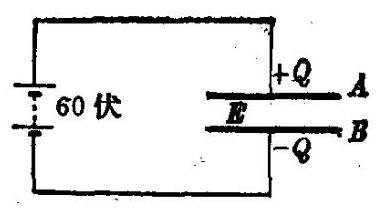
\includegraphics[max width=0.4\textwidth]{images/01913056-1f15-74d8-9184-9aab52c9d66b_35_655333.jpg}
\end{center}

图 1-22

解这道题时可以这样分析: 金属板间的电势差就是电池组的电压. 知道这个电势差 \(U\) 后,可以用公式 \(E = U/d\) 计算出场强 \(E\) .

\[
E = \frac{U}{d} = \frac{60}{3 \times {10}^{-2}}\text{ 伏 }/\text{ 米 } = 2 \times {10}^{3}\text{ 伏 }/\text{ 米. }
\]

\(A\) 板带正电, \(B\) 板带负电,所以场强方向是由 \(A\) 板指向 \(B\) 板.

\section*{练习六}

(1)在匀强电场中,沿电场强度的方向依次排列着 \(A\text{、}B\) 、 \(C\) 三点, \(A\text{、}B\) 间的距离是 4.0 厘米, \(B\text{、}C\) 间的距离是 6.0 厘米. \(A\) 点的电势最高,设电场强度是 \({1.5} \times {10}^{4}\) 伏/米,试求 \(A\) 与 \(B\) 、 \(B\) 与 \(C\text{、}A\) 与 \(C\) 间的电势差.

(2)有两块相距 10 厘米的平行的金属板, 两板间的电压为 9000 伏. 求两板间的电场强度. 若在两板间与两板等距离的一点上有一颗带着 \(- {1.6} \times {10}^{-7}\) 库电量的尘埃,求这颗尘埃受到的电场力. 当它移动到带正电的那块金属板时, 电场力做了多少功?

\section*{八、带电粒子在匀强电场中的运动}

带电粒子在电场中要受到电场力的作用, 因此要产生加速度, 速度的大小和方向都可以发生变化. 在现代科学实验和技术设备中, 常常根据这个道理, 利用电场来改变或控制带电粒子的运动. 这种应用大致可以分成两种情况. 一是利用电场来使带电粒子加速, 一是利用电场来使带电粒子偏转.

带电粒子的加速 如图 1-23 所示, 在真空中有一对平行金属板,由于接上电压为 \(U\) 的电池组而带电,在它们之间建立了匀强电场. 设在电场力的作用下,有一个电量为 \(q\) 的静止的带电粒子, 从一个极板移动到另一个极板. 根据以前学过的知识可以知道, 带电粒子减少的电势能 \(\Delta \mathcal{E} = {qU}\) 应该等. 于粒子获得的动能. 如果带电粒子的质量是 \(m\) ,到达另一极板时的速度是 \(v\) ,就有

\[
\frac{1}{2}m{v}^{2} = {qU}
\]

\begin{center}
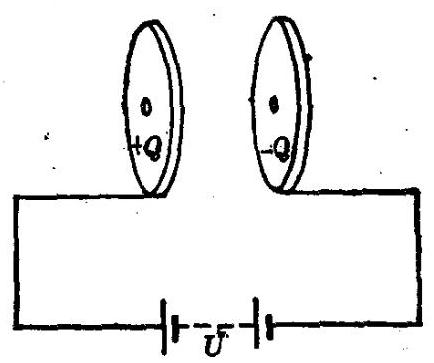
\includegraphics[max width=0.5\textwidth]{images/01913056-1f15-74d8-9184-9aab52c9d66b_37_632735.jpg}
\end{center}

图 1-23

利用上面的关系式, 如果知道被加速的带电粒子的质量 \(m\) 和电量 \(q\) ,还知道平行金属板间的电压 \(U\) ,就可以计算出带电粒子被加速后的速度 \(v = \sqrt{\frac{2qU}{m}}\) .

在图 1-23 的两个极板上, 各有一个小孔, 彼此正对. 如果在正极板的左侧有一些带电量为 \(+ q\) 的粒子,其中有一部分能以很小的速度从左孔进入电场被加速, 就将以 \(v = \sqrt{\frac{2qU}{m}}\) 的速度从右孔穿出. 由于在带电平行板之外没有电场, 从右孔穿出的带电粒子, 将做匀速直线运动, 直到它们碰到别的物体或者进入另一个电场为止.

带电粒子的偏转 如图 1-24 所示, 在真空中水平放置一对金属板,板间的距离为 \(d\) . 接上电压为 \(U\) 的电池组后,在它们之间就建立了匀强电场,场强为 \(E = \frac{U}{d}\) . 当速度为 \({v}_{0}\) 、带

\begin{center}
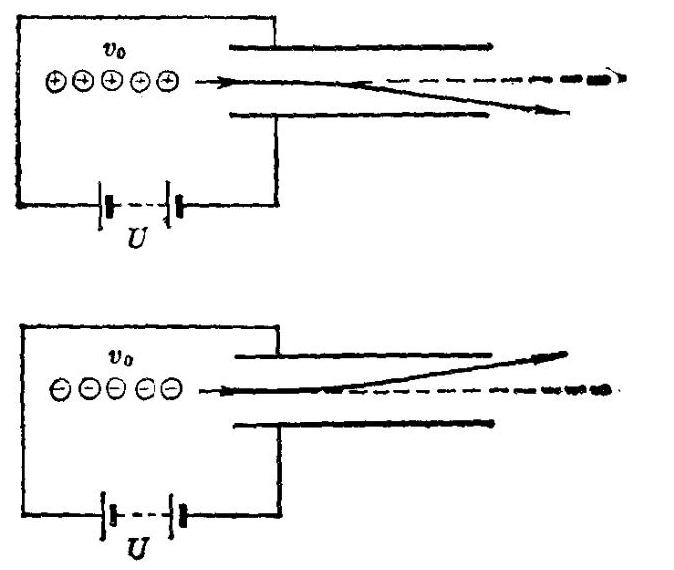
\includegraphics[max width=0.7\textwidth]{images/01913056-1f15-74d8-9184-9aab52c9d66b_38_644084.jpg}
\end{center}

图 1-24

电量为 \(q\) 的带电粒子沿着水平方向进入这个电场时,由于在竖直方向上受到电场力 \({qE}\) 的作用,带电粒子的运动将跟水平抛出的物体的运动相似: 在水平方向上做匀速运动, 在竖直方向上做初速度为零的匀加速运动. 因此, 我们可以用运动合成的知识来求粒子在任一时刻的速度. 下面我们通过一道例题来研究带电粒子的偏转问题.

[例题] 一对长 6.0 厘米、相距 0.20 厘米的平行金属板, 加上 2.0 伏的电压,产生一个电场. 速度为 \({3.0} \times {10}^{7}\) 米/秒的电子流, 以平行于极板的方向进入电场. 求电子离开电场时, 偏离原来方向的角度有多大(图 1-25).

\begin{center}
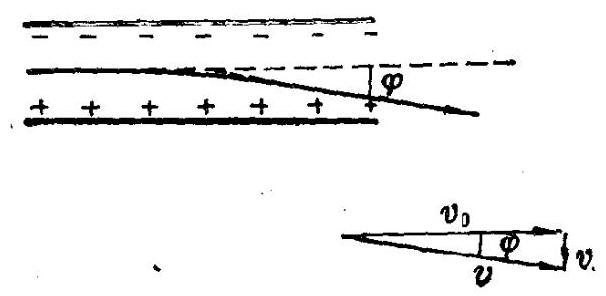
\includegraphics[max width=0.6\textwidth]{images/01913056-1f15-74d8-9184-9aab52c9d66b_38_558921.jpg}
\end{center}

图 1-25

由于电子在水平方向做匀速运动, 所以通过极板需要的时间 \(t\) ,可以由极板的长度 \(l\) 和电子进入极板时的速度 \({v}_{0}\) 求出.

由于电子在竖直方向做初速度为零的匀加速运动, 所以离开电场那一时刻在竖直方向上的分速度 \({v}_{ \bot } = {at}\) . 式中的加速度 \(a\) 可由 \(a = \frac{F}{m}\) 和 \(F\;e \cdot E = e \cdot \frac{U}{d}\) 求出.

知道了 \({v}_{ \bot }\) 和 \({v}_{0}\) ,就可以由

\[
\operatorname{tg}\phi = \frac{{v}_{1}}{{v}_{0}}
\]

求出电子离开电场时偏转的角度 \(\phi\) .

解: 电子飞越电场的时间 \(t = \frac{l}{{v}_{0}}\) .

在电场中, 由于在竖直方向的加速度为

\[
a = \frac{eE}{m} = \frac{eU}{md}
\]

电子离开电场时在竖直方向的分速度为

\[
{v}_{ \bot } = \frac{eU}{md}t = \frac{eUl}{{md}{v}_{0}}.
\]

由于 \(l = {6.0} \times {10}^{-2}\) 米, \(d = {0.20} \times {10}^{-2}\) 米, \(U = {2.0}\) 伏, \(e = {1.60} \times {10}^{-{19}}\) 库, \(\;m = {0.91} \times {10}^{-{30}}\) 千克, \(\;{v}_{0} = {3.0} \times {10}^{7}\) 米/秒. 所以,

\[
{v}_{ \bot } = \frac{{1.60} \times {10}^{-{19}} \times {2.0} \times {6.0} \times {10}^{-2}}{{0.91} \times {10}^{-{30}} \times {0.20} \times {10}^{-2} \times {3.0} \times {10}^{7}}\text{ 米 }/\text{ 秒 }
\]

\(= {3.5} \times {10}^{5}\) 米 \(/\) 秒.

\[
\operatorname{tg}\phi = \frac{{v}_{ \bot }}{{v}_{0}} = \frac{{3.5} \times {10}^{5}}{{3.0} \times {10}^{7}} = {0.0117},
\]

\[
\phi = {0.67}^{ \circ }\text{.}
\]

\section*{练 习 七}

(1) 一个初速度为零的电子,在场强为 \({4.0} \times {10}^{3}\) 伏 \(/\) 米的匀强电场中被加速. 求经过 \({2.0} \times {10}^{-8}\) 秒后,电子的速度和动能.

(2)在真空中有一对平行金属板, 相距 6.2 厘米, 加上 90 伏的电压. 两价的氧离子从静止出发被加速, 从一板到达另一板时, 它的动能是多少?

(3)在本节例题中, 如果极板的长度、极板间的距离和被偏转的电子流的初速度都不变, 电子流的偏转角的大小取决于什么?

(4)在本节例题中的电子流离开极板时, 在竖直方向上移动了多大距离? 离开极板时电子流的速度是多大?

\section*{九、示 波 管}

示波管是示波器的核心部件. 现在, 示波器已经成为科学研究、检测和修理各种电子仪器不可缺少的工具. 我们在分组实验中将学习它的使用方法. 在这一节里先学习示波管的结构和工作原理.

示波管由电子枪、偏转电极和荧光屏组成 (图 1-26), 它的内部是真空.

\begin{center}
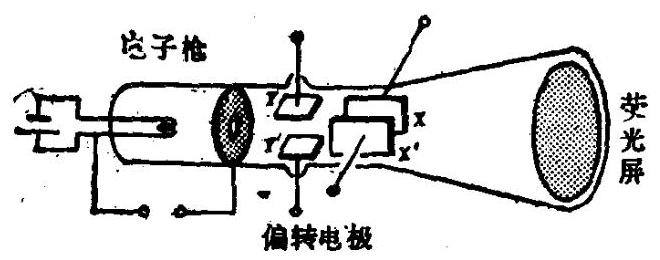
\includegraphics[max width=0.7\textwidth]{images/01913056-1f15-74d8-9184-9aab52c9d66b_41_763965.jpg}
\end{center}

图 1-26

电子枪是由发射电子的炽热金属丝和加速电极组成的. 图 1-27 是示波管的电子枪示意图. 在炽热的金属丝前面有带孔的金属板. 金属丝和金属板之间是加速电子的电场. 从炽热金属丝发射出来的电子被加速后从金属板的小 孔 穿出, 沿着直线前进, 最后打在荧光屏上, 在那里产生一个小的亮斑.

\begin{center}
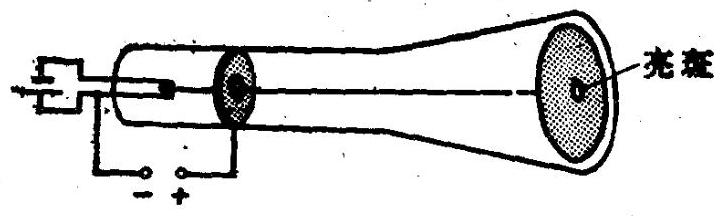
\includegraphics[max width=0.8\textwidth]{images/01913056-1f15-74d8-9184-9aab52c9d66b_41_377360.jpg}
\end{center}

图 1-27 电子枪示意图

图 1-26 中电子枪前面的一对偏转电极 \(Y\text{、}{Y}^{\prime }\) 叫做竖直偏转板. 在 \(Y\text{、}{Y}^{\prime }\) 上加电压,使 \(Y\) 板的电势高于 \({Y}^{\prime }\) 板,场强方向由 \(Y\) 指向 \({Y}^{\prime }\) ,电子枪射出的电子流就要向 \(Y\) 板偏转,荧光屏上的亮斑将偏到原来位置的上方. 如果加速电子的电场不变, 即保持从电子枪射出的电子流的速度不变, 从上节的例题可以知道,亮斑偏移的大小,跟加在 \(Y\text{、}{Y}^{\prime }\) 上的电压的大小成正比. 所以示波管可以用来测量电压.

如果在 \(Y\text{、}{Y}^{\prime }\) 上所加的电压是变化的,那么荧光屏上的亮斑就会在竖直方向上随着电压的变化而改变位置. 当电压是周期性变化的, 而且变化又很快的时候, 荧光屏上亮斑位置的往返移动也会很快, 看起来就成了一条竖直的亮线. 这样, 就看不出电压是怎样随时间而变化的了. 为了在上述情况下也能观察电压是怎样随时间而变化的,要在另一对偏转电极 \(X\) 、 \({X}^{\prime }\) 一水平偏转板上加一个扫描电压.

我们可以通过下面的比喻来了解扫描电压的作用. 当你拿着香火在竖直方向上抖动时, 看到的只是一条竖直的亮线. 如果在抖动香火的同时还使香火沿着水平方向匀速移动, 香火描绘出来的亮线就能显示出它在竖直方向上抖动的情况. 在水平偏转板 \(X\text{、}{X}^{\prime }\) 上加扫描电压,可以使亮斑从左向右匀速地水平移动, 这叫做扫描. 当亮斑移到右端以后, 又会立即回到左端,开始第二次扫描. 如果在 \(X\text{、}{X}^{\prime }\) 上加扫描电压的同时,在 \(Y\text{、}{Y}^{\prime }\) 上加随时间而变化的电压,我们就可以在荧光屏上看到由亮斑的移动描绘出来的曲线, 这条曲线可以显示出偏转板 \(Y\text{、}{Y}^{\prime }\) 上的电压随时间而变化的情况. 图 1-28 表示的是加在竖直偏转板上的交流电压随时间变化的情况.

\begin{center}
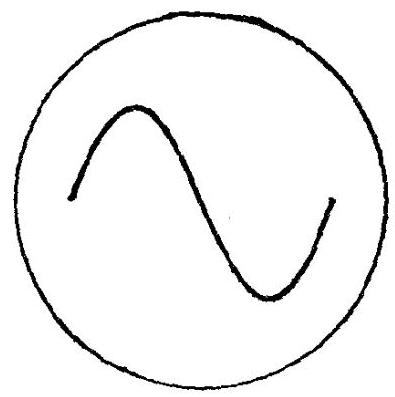
\includegraphics[max width=0.4\textwidth]{images/01913056-1f15-74d8-9184-9aab52c9d66b_42_664272.jpg}
\end{center}

图 1-28

示波管的突出优点是它的反应很快. 电子的质量很小, 惯性也就很小, 因此, 示波管能够灵敏地反映出加在偏转板上的极其迅速而又微小的电压变化, 并把它显示在荧光屏上、

\section*{十、电容器 电容}

电容器 任何两个彼此绝缘而又互相靠近的导体, 都可以看成是一个电容器. 这两个导体就是电容器的两个极. 我们在前面多次讲过的两块正对的、互相平行的、相隔很近的、 彼此绝缘的金属板, 就组成一个最简单的电容器, 叫做平行板电容器.

使电容器带电叫做充电, 这时总是使它的一个导体带正电, 另一个导体带等量的负电. 每个导体所带电量的绝对值, 叫做电容器所带的电量. 把平行板电容器的一个极板接电池组的正极, 另一个极板接电池组的负极, 两个极板就分别带上等量的异种电荷. 充 \(f\) 电的电容器的两极之间有电场.

使充电后的电容器失去电荷叫做放电. 用一根导线把电容器的两极接通, 两极上的电荷互相中和, 电容器就不带电了. 放电后两极之间不再存在电场.

电容器是电气设备中的重要元件之一, 在电子技术和电工技术中有很重要的应用. 我们在后面的第五章到第七章中将会遇到一些它的应用.

电容 电容器带电的时候, 它的两极之间要产生电势差. 对任何一个电容器来说, 两极间的电势差都随所带电量的增加而增加, 而且电量跟电势差成正比, 它们的比值是一个恒量. 不同的电容器,这个比值一般是不同的. 在 \(U\) 相同的条件下, 这个比值越大的电容器所带的电量越多, 因而这个比值表征了电容器容纳电荷的本领, 我们称这个比值为电容器的电容.

如果用 \(Q\) 表示电容器所带的电量,用 \(U\) 表示它的两极间的电势差,用 \(C\) 表示它的电容,那么

\[
C - \frac{Q}{U}
\]

在国际单位制里, 电容的单位是法拉, 简称法, 国际符号是 \(\mathrm{F}\) . 一个电容器,如果带 1 库的电量时两极间的电势差是 1 伏, 这个电容器的电容就是 1 法.

\[
\text{1 法} = 1\text{库/伏.}
\]

法这个单位太大,实际上常用较小的单位: 微法 \(\left( {\mu \mathrm{F}}\right)\) 和皮法 \(\left( \mathrm{{pF}}\right)\) . 它们间的换算关系是:

1 法 \(= {10}^{6}\) 微法 \(= {10}^{12}\) 皮法.

无线电收音机里常用的电容器, 电容从几个皮法到几十个微法的都有.

\section*{练 习 八}

(1) 一个电容为 100 微法的电容器, 用 6 伏的电池组给它充电, 它带的电量是多少? 如果改用 3 伏的电池组给它充电, 它带的电量又是多少?

(2)某电容器带电 \({1.0} \times {10}^{-5}\) 库时,两极间的电势差是 200 伏,如再增加电量 \({1.0} \times {10}^{-5}\) 库,两极间的电势差将变为多少? 在这个过程中电容器的电容有没有变化?

(3)电容是 50 微法的电容器,带电量是 \({1.5} \times {10}^{-8}\) 库时, 两极间的电势差是多大? 如果带电量增大到原来的 10 倍, 两极间的电势差又是多大?

\section*{十一、平行板电容器的电容 常用电容器}

平行板电容器的电容 现在我们来研究平行板电容器的电容跟哪些因素有关.

如图 1-29 所示,让平行板电容器带电后,用静电计 \(\Phi\) 来测量两极板 \(A\text{、}B\) 间的电势差. 不改变 \(A\text{、}B\) 两极板所带的电量, 只改变两极板间的距离, 可以看到, 距离越大, 静电计指出的电势差越大. 这表示平行板电容器的电容随两板距离的增大而减小.

\begin{center}
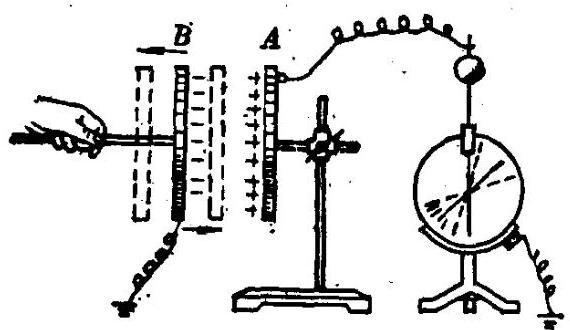
\includegraphics[max width=0.6\textwidth]{images/01913056-1f15-74d8-9184-9aab52c9d66b_45_420456.jpg}
\end{center}

图 1-29

如图 1-30 所示, 不改变两极板所带电量和它们的距离, 只改变两极板的正对面积, 可以看到, 正对面积越小, 静电计指出的电势差越大. 这表示平行板电容器的电容随两板的正对面积的减小而减小.

\begin{center}
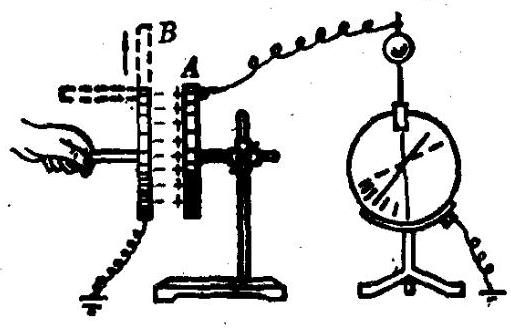
\includegraphics[max width=0.5\textwidth]{images/01913056-1f15-74d8-9184-9aab52c9d66b_45_946371.jpg}
\end{center}

图 1-30

\customfootnote{

① 静电计是在验电器的基础上制成的, 用来测量导体间的电势差. 使用时把它的金属球跟一个导体连接, 把它的金属外壳跟另一个 导体连接或同时接地, 从指针的偏转角度就可以知道两个导体间的电势差.

}

\begin{center}
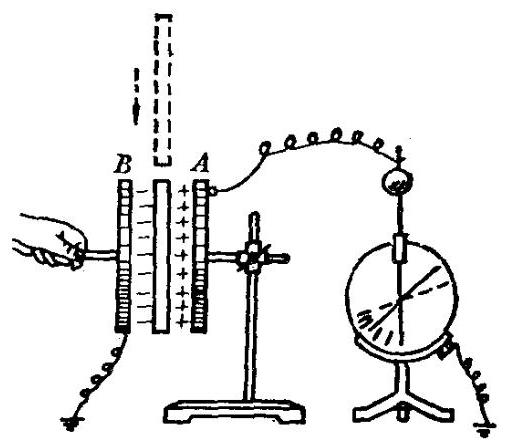
\includegraphics[max width=0.5\textwidth]{images/01913056-1f15-74d8-9184-9aab52c9d66b_46_932097.jpg}
\end{center}

图 1-31

如图 1-31 所示, 保持两极板所带电量、它们的距离、 它们的正对面积都不改变, 只在极板间插入一块绝缘休一 又叫电介质, 可以看到, 静电计指出的电势差要减小. 这表示平行板电容器的电容由于插入电介质而增大. 电容器极板间充满某种电介质时电容增大的倍数就叫做这种电介质的介电常数. 下面是几种电介质的介电常数的值:

\begin{center}
\adjustbox{max width=\textwidth}{
\begin{tabular}{|c|c|c|c|c|c|}
\hline
电介质 & 空 'i & 有 蜡 & 陶瓷 & 玻 璃 & 2. b) \\
\hline
介电常数 & 1.0005 & \({2.0} \sim {2.1}\) & 6 & \(4 \sim {11}\) & \(6 \sim 8\) \\
\hline
\end{tabular}
}
\end{center}

理论分析证明, 平行板电容器的电容, 跟介电常数成正比, 跟正对面积成正比, 跟极板的距离成反比. 这跟上面实验研究的结果是完全一致的.

一般说来, 电容器的电容是由两个导体的大小和形状、两个导体的相对位置以及它们间的电介质决定的.

常用电容器 懂得了决定电容大小的因素. 就可以利用这些知识来改变电容器的电容。实际上,人们正是这样制成各种电容器, 来满足不同需要的. 从构造上看, 常用的电容器可分为固定电容器和可变电容器两类.

固定电容器的电容是固定不变的, 由于所用的电介质不同, 又可分为纸质电容器、云母电容器、瓷电容器、电解电容器等. 下面我们说明一下纸质电容器和电解电容器.

纸质电容器是在两层锡箔或铝箔中间夹以在石蜡中浸过的纸, 一起卷成圆柱体而制成的 (图 1-32). 纸浸过石蜡后, 可以避免潮气侵入, 大大增强绝缘能力. 改变锡箔或铝箔的面积, 可以制成电容大小不同的纸质电容器. 这种电容器的特点是容易制造出电容较大的电容器, 而且价格较低.

电解电容器的外形如图 1-33 所示. 在这种电容器中, 是用铝箔作阳极, 用铝箔上很薄的一层氧化膜 (它有很好的绝缘性能) 作电介质, 用浸渍过电解液的纸作阴极制成的. 由于氧化膜很薄, 这种电容器的电容较大. 电解电容器的极性是固定的, 使用时正负极不能接错, 也不能接交流电.

\begin{center}
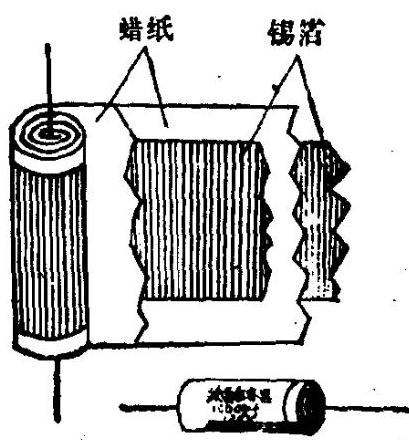
\includegraphics[max width=0.4\textwidth]{images/01913056-1f15-74d8-9184-9aab52c9d66b_47_534512.jpg}
\end{center}

图 1-32 纸质电容器

\begin{center}
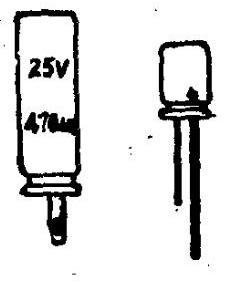
\includegraphics[max width=0.2\textwidth]{images/01913056-1f15-74d8-9184-9aab52c9d66b_47_838616.jpg}
\end{center}

\begin{center}
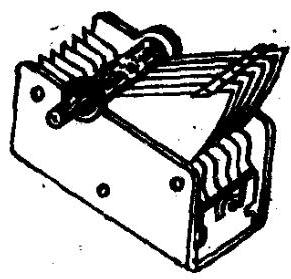
\includegraphics[max width=0.3\textwidth]{images/01913056-1f15-74d8-9184-9aab52c9d66b_47_445999.jpg}
\end{center}

图 4-34 可变电容器

图 1-33 电解电容器

可变电容器的电容是可以改变的, 它由两组铝片组成 (图 1-34), 固定不动的一组铝片叫定片, 可以转动的一组铝片叫动片. 在定片和动片之间, 通常是空气, 也有用电介质薄片的. 转动动片, 两组铝片的正对面积发生变化, 电容也随着改变.

\begin{center}
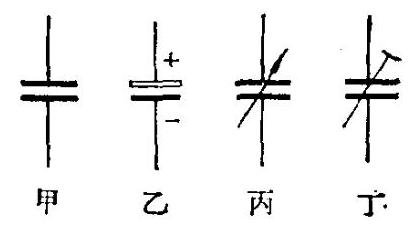
\includegraphics[max width=0.4\textwidth]{images/01913056-1f15-74d8-9184-9aab52c9d66b_48_469817.jpg}
\end{center}

图 1-35 甲: 固定电容器. 乙: 电解电容器. 丙: 可变电容器. 丁: 半可变电容器

此外还有半 可变 电容器, 能微小地调整两极片间的距离或改变它们的正对面积, 使电容发生微小改变. 图 1-35 是电路图中常用的儿种电容器的符号.

加在电容器两极上的电压, 不能超过某一限度. 超过这个限度, 电介质将被击穿, 电容器就被损坏, 这个极限电压叫做击穿电压, 电容器长期有效工作时的最大电压一, 额定电压应该低于击穿电压. 电容器上一般都标明了电容和额定电压的数值.

\section*{十二、电容器的连接*}

在实际使用电容器时, 有时会遇到电容器的电容不够或耐压能力不够的问题, 这就需要把几个电容器连接起来使用, 连接的基本方法有串联和并联两种.

电容器的串联 把几个电容器的极首尾相接, 连成一串, 这就是电容器的串联. 图 1-36 是电容分别为 \({C}_{1}\text{、}{C}_{2}\text{、}{C}_{3}\) 的三个电容器的串联. 把串联好的电容器接到电压为 \(U\) 的电源上 (图 1-37). 如果两端的极板带的电量分别为 \(+ Q\) 和 \(- Q\) ,由

\begin{center}
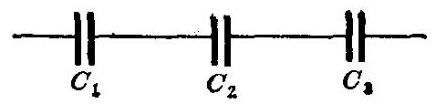
\includegraphics[max width=0.5\textwidth]{images/01913056-1f15-74d8-9184-9aab52c9d66b_48_705439.jpg}
\end{center}

图 1-36 电容器的串联

于静电感应, 中间各极板所带的电量也等于 \(+ Q\) 或 \(- Q\) ,所以串联时每个电容器带的电量都是 \(Q\) . 如果各个电容器的电压分别为 \({U}_{1}\text{、}{U}_{2}\text{、}{U}_{3}\) ,就有

\[
{U}_{1} = \frac{Q}{{C}_{1}},\;{U}_{2} = \frac{Q}{{C}_{2}},\;{U}_{3} = \frac{Q}{{C}_{3}}.
\]

\begin{center}
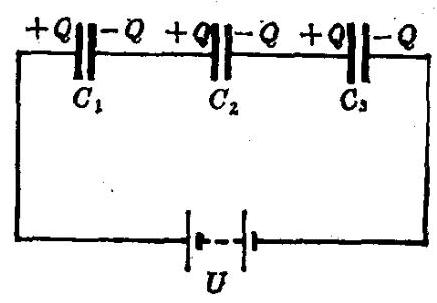
\includegraphics[max width=0.5\textwidth]{images/01913056-1f15-74d8-9184-9aab52c9d66b_49_766231.jpg}
\end{center}

图 1-37

由于总电压 \(U\) 等于各个电容器上的电压之和,所以,

\[
U = {U}_{1} + {U}_{2} + {U}_{3} = Q\left( {\frac{1}{{C}_{1}} + \frac{1}{{C}_{2}} + \frac{1}{{C}_{3}}}\right) .
\]

设串联电容器的总电容为 \(C\) ,则 \(U = \frac{Q}{C}\) ,所以,

\[
\therefore \frac{1}{C} = \frac{1}{{C}_{1}} + \frac{1}{{C}_{2}} + \frac{1}{{C}_{3}}\text{.}
\]

这就是说, 串联电容器的总电容的倒数等于各个电容器的电容的倒数之和. 电容器串联之后, 相当于增大了两极的距离, 因此总电容小于每个电容器的电容.

电容器的并联 把几个电容器的正极连在一起, 负极也连在一起,这就是电容器的并联. 图 1-38 是电容分别为 \({C}_{1}\) 、 \({C}_{2}\text{、}{C}_{3}\) 的三个电容器的并联.

\begin{center}
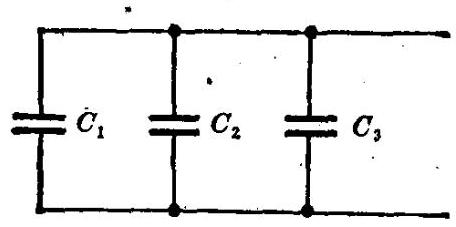
\includegraphics[max width=0.5\textwidth]{images/01913056-1f15-74d8-9184-9aab52c9d66b_49_640946.jpg}
\end{center}

图 1-38 电容器的并联

把并联好的电容器接到电压为 \(\underline{U}\) 的电源上 (图 1-39),每个电容器的电压都是 \(U\) . 如果各个电容器所带的电量分别为 \({Q}_{1}\text{、}{Q}_{2}\text{、}{Q}_{3}\) ,那么, \({Q}_{1}\;{C}_{1}U,{Q}_{2} = {C}_{2}U,{Q}_{3}\;{C}_{3}U\) . 由于电容器组贮存的总电量 \(Q\) 等于各个电容器所带电量之和,所以,

\[
Q + {Q}_{1} + {Q}_{2} + {Q}_{3}\;\left( {{C}_{1} + {C}_{2} + {C}_{3}}\right) U.
\]

\begin{center}
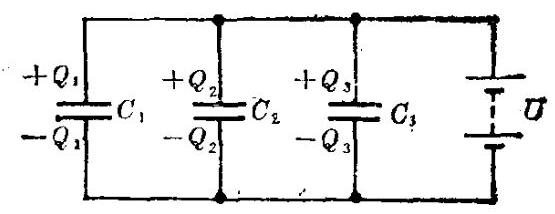
\includegraphics[max width=0.6\textwidth]{images/01913056-1f15-74d8-9184-9aab52c9d66b_50_240382.jpg}
\end{center}

图 1-39

设并联电容器的总电容为 \(C\) ,则 \({QCU}\) ,所以,

\[
\smallsetminus C\;{C}_{1} \mid {C}_{2} \mid {C}_{3}
\]

这就是说, 并联电容器的总电容等于各个电容器的电容之和. 电容器并联之后, 相当于增大了两极的面积, 因此总电容大于每个电容器的电容.

可以看出, 电容器串联后, 电容减小了, 但耐压能力提高了, 所以要承受较高的电压时, 可以把电容器串联起来; 电容器并联后, 电容增大了, 耐压能力没有提高, 所以在需要大电容时, 可以把电容器并联起来.

\section*{十三、静电的防止和应用}

静电的防止 摩擦产生的静电, 在生产、生活上给人们带来很多麻烦。 甚至造成危害.

印刷厂里, 纸页之间的摩擦起电, 会使纸页粘在一起, 难于分开, 给印刷带来麻烦. 印染厂里, 棉纱、毛线、人造纤维上的静电, 会吸引空气中的尘埃, 使印染质量下降. 干干净净的人造纤维服装, 穿不了多大功夫就会蒙上一层灰尘, 也是由于静电吸引尘埃的缘故.

静电荷积累到一定程度, 会产生火花放电, 带来不幸. 在地毯上行走的人, 与地毯摩擦而带的电如果足够多, 当他伸手去拉金属门把手时, 手与金属把手 (上面有感应电荷) 间会产生火花放电, 严重时会使他惊厥. 在空气中飞行的飞机, 与空气摩擦而带的电如果在着陆过程中没有导走, 当地勤人员接近机身时, 人与飞机间可能产生火花放电, 严重时可能将人击倒. 专门用来装汽油或柴油等液体燃料的卡车, 在灌油、运输过程中, 燃油与油罐摩擦、撞击而带电, 如果没有及时导走, 积累到一定程度, 会产生电火花, 引起爆炸.

防止静电危害的基本办法, 是尽快把产生的静电导走, 避免越积越多. 具体措施则多种多样. 油罐车是靠一条拖在地上的铁链把静电导走. 飞机机轮上通常都装有搭地线, 也有用导电橡胶做机轮轮胎的, 着陆时它们可将机身的静电导入地下. 在地毯中夹杂 \({0.05} \sim {0.07}\) 毫米的不锈钢丝导电纤维, 消除静电的效果很好. 在印染厂中保持适当的湿度, 潮湿的空气可使静电荷很快消失.

静电的应用 静电也可以用来为物质文明和精神文明建设服务. 目前, 静电的应用已有多种, 但依据的物理原理几乎都是让带电的物质微粒在电场力作用下, - 奔向并吸附到电极上. 下面介绍比较常见的静电除尘和静电复印.

以煤为燃料的工厂、电站, 每天排出的烟带走大量的煤

粉, 不仅浪费燃料, 而且造成严重的环境污染. 可以利用图 1-40 所示的静电除尘 器 消 除烟气中的煤粉. 除尘器由金属管 \(A\) 和悬在管中的金属丝 \(B\) 组成, \(A\) 接到高压电源正极, \(B\) 接到高压电源负极. \(A\text{、}B\) 之间有很强的电场,而且距 \(B\) 越近电场越强. \(B\) 附近的空气分子被强电场电离为电子和正离子. 正离子跑到 \(B\) 上得到电子又变成空气分子. 电子奔向正极 \(A\) 的过程中, 遇到烟气中的煤粉, 使煤粉带负电,吸附到正极 \(A\) 上, 排出的烟就成为清洁的了.

\begin{center}
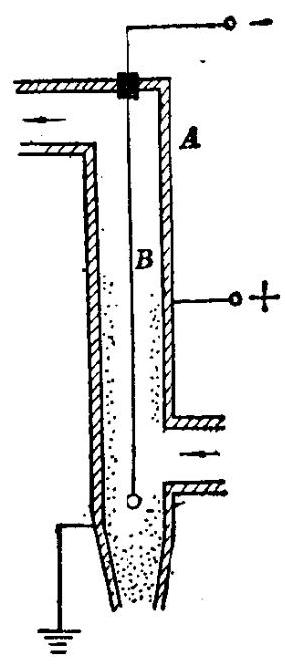
\includegraphics[max width=0.3\textwidth]{images/01913056-1f15-74d8-9184-9aab52c9d66b_52_153305.jpg}
\end{center}

图 1-40 静电除尘器示意图

静电复印可以迅速、方便地把图书、资料、文件复印到纸上. 静电复印机的中心部件, 是一个可以旋转的接地的铝辊, 表面镀着一层半导体硒, 叫做硒鼓. 半导体硒有特殊的光电性质, 没有光线照射时是很好的绝缘体, 能保持电荷, 受到光的照射就立刻变成导体, 将所带的电荷导走.

复印每一页书稿都要经过充电、曝光、显影、转印等几个步骤, 这些步骤是在硒鼓转动一周的过程中依次完成的.

充电: 由电源使硒鼓表面带上正电荷.

曝光: 利用光学系统将原稿上字迹的像成在硒鼓上 (图 1-41). 硒鼓上字迹的像实际是没有光照射的地方, 保持着正电荷, 而其它地方受到了光线照射, 正电荷被导走. 这样, 硒

\begin{center}
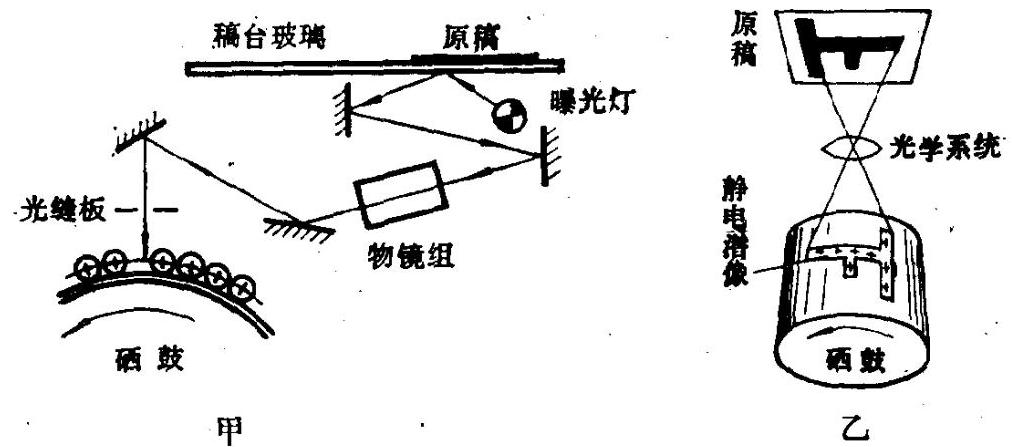
\includegraphics[max width=1.0\textwidth]{images/01913056-1f15-74d8-9184-9aab52c9d66b_53_340113.jpg}
\end{center}

图 1-41 曝光

鼓上就留下了字迹的“静电潜像”.

显影: 带负电的墨粉被带正电的“静电潜像”吸引, 并吸附在潜像上 (图 1-42), 显出墨粉组成的字迹.

\begin{center}
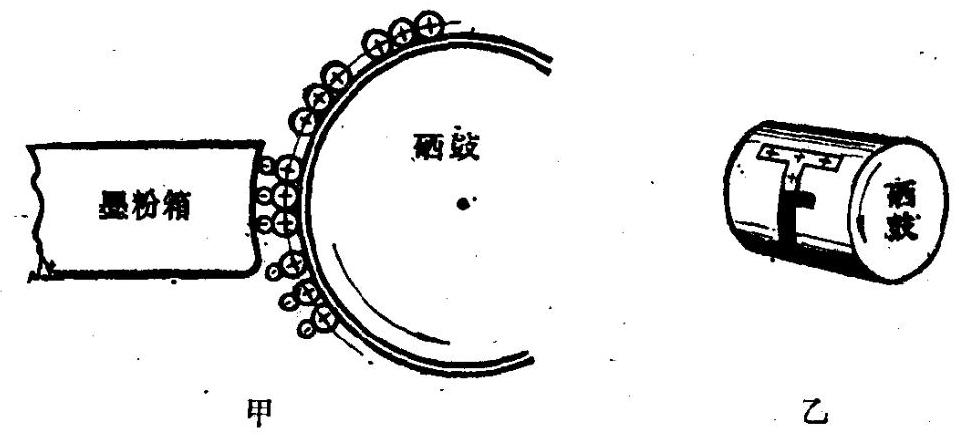
\includegraphics[max width=1.0\textwidth]{images/01913056-1f15-74d8-9184-9aab52c9d66b_53_472283.jpg}
\end{center}

图 1-42 显影

转印: 带正电的转印电极使输纸机构送来的白纸带正电. 带正电的白纸与硒鼓表面墨粉组成的字迹接触, 将带负电的墨粉吸到白纸上(图 1-43).

此后, 吸附了墨粉的纸被送入定影区, 墨粉在高温下熔化, 浸入纸中, 形成牢固的字迹; ’硒鼓则经过清除表面残留的墨粉、电荷, 准备迎接下一页书稿的复印.

\begin{center}
\includegraphics[max width=1.0\textwidth]{images/01913056-1f15-74d8-9184-9aab52c9d66b_54_512568.jpg}
\end{center}

图 1-13 转印

图 1-11 表示出了复印的全过程.

\begin{center}
\includegraphics[max width=1.0\textwidth]{images/01913056-1f15-74d8-9184-9aab52c9d66b_54_621416.jpg}
\end{center}

图 1-44 复印程序

\section*{小实验}

象图 1-45 那样在桌上放两摞书, 把一块洁净的玻璃垫起来,使玻璃离开桌面 \(2 \sim 3\) 厘米. 在宽 0.5 厘米的纸条上画出各种舞姿的人形, 用剪刀把它们剪下来, 放在玻璃下面. 然后用一块硬泡沫塑料在玻璃上擦, 就可以看到小纸人翩翩起舞了. 请你注意观察现象, 并想想产生现象的原因, 如果实验前用一根火柴把“跳舞区”烤一烤, 实验效果就会更好. 如果向 “跳舞区”哈一口气, 小纸人跳得就不活跃或者不能起舞了. 试试看, 从这里你能找到一种防止静电危害的方法吗?

\begin{center}
\includegraphics[max width=0.7\textwidth]{images/01913056-1f15-74d8-9184-9aab52c9d66b_55_729208.jpg}
\end{center}

图 1-45

找一根导线, 一端粘在玻璃上, 另一端接地, 再用硬泡沫塑料擦玻璃, 小纸人还起舞吗? 想想看在这种情况下用接地的方法能防止静电的产生吗?

\section*{复习 题}

(1)库仑定律的内容是什么? 写出它的公式. 写出在国际单位制中静电力恒量的表示式.

(2)什么是电场强度? 怎样求电场中某点的场强大小? 电场的方向是怎样规定的? 写出点电荷在真空中的场强公式.

(3)什么是电势能? 在电场中移动电荷时, 什么情况下电势能增加, 什么情况下电势能减少?

(4)什么是电势差 \(\mathfrak{r}\) 知道了电场中两点间的电势差,怎样计算在这两点间移动电荷时电势能的变化或需要做的功? 在匀强电场中电势差跟电场强度有什么关系?

(5)什么是电势? 怎样求电场中某点的电势?

(6)电力线为什么一定跟等势面垂直, 而且总是由电势高的地方指向电势低的地方?

(7)说明用电场使带电粒子加速和偏转的原理.

(8)什么叫电容器的电容? 写出它的公式.

(9) 串联电容器的总电容等于什么? 并联电容器的总电容等于什么? 在什么情况下需要把电容器串联起来? 在什么情况下需要把电容器并联起来?

\section*{习 题}

(1)在真空中两个点电荷, 它们间的相互作用力在下列情况下将如何变化? ①一个电荷的电量变为原来的 2 倍; ② 两个电荷的电量都减小到原来的 \(1/2\) ; ③ 电荷间距离加倍.

(2)两个相同的金属球, 一个带的电量为 \(+ {4.0} \times {10}^{-7}\) 库,一个带的电量为 \(- {6.0} \times {10}^{-7}\) 库,求

\begin{center}
\includegraphics[max width=0.3\textwidth]{images/01913056-1f15-74d8-9184-9aab52c9d66b_57_908319.jpg}
\end{center}

图 1-46

① 两球相距 50 厘米时的作用力.

② 把两球接触后, 再使它们相距 50 厘米时的作用力 (参看图 1-46).

(3) 已知电子的质量是 \({0.91} \times\) \({10}^{-{30}}\) 千克,质子的质量是 \({1.67} \times {10}^{-{27}}\) 千克. 电子和质子间的静电力是它们之间万有引力的多少倍?

(4)从一点用两根长 4.0 厘米的丝线吊 起两个质量都是 0.10 克的小导体球. 球上带着等量、同号的电荷. 两球互相排斥的结果使丝线跟竖直线所成的角是 \({30}^{ \circ }\) . 求两个导体球间作用的电力的大小和导体球上的带电量.

(5)在一条直线上依次排列着三个固定不动的电荷 \({Q}_{1}\) 、 \({Q}_{2}\text{、}{Q}_{3}\) ,它们的电量分别为 +10 微库,-20 微库 和 -10 微库. 其中 \({Q}_{2}\) 与 \({Q}_{1}\) 相距 \(5\) 米, \({Q}_{3}\) 与 \({Q}_{2}\) 相距 10 米,求作用在 \({Q}_{2}\) 上的电力的大小和方向.

(6) 一对带等量异号电荷的平行金属板 相距 1.0 厘米, * 在带负电的那块金属板处, 有一个初速度为零的电子, 经过 \({1.0} \times {10}^{-9}\) 秒到达了带正电的那块金属板. 这个电子受 到 的电场力是多大? 板间的电场强度是多大?

(7)在两个水平放置的金属板之间. 有一个勾强电场, 它的场强是 \({1.5} \times {10}^{5}\) 牛/库,方向竖直向下. 现在,有一个质量为 \({1.0} \times {10}^{-9}\) 千克的液滴在这个电场中处于平衡状态. 这个液滴带正电还是负电? 它带的电量是多少?

(8)一个平行板电容器两板相距 2 厘米 (图 1-47), 两板间的场强是 \({1.6} \times {10}^{3}\) 伏/米,点 \(A\) 距下板 1.5 厘米,点 \(B\) 距下. 、板 0.5 厘米,下板接地,求 \(A\text{、}B\) 两点的电势各是多少?

\begin{center}
\includegraphics[max width=0.4\textwidth]{images/01913056-1f15-74d8-9184-9aab52c9d66b_58_602752.jpg}
\end{center}

图 1-47

(9)在研究原子物理的时候, 常用电子伏特, 简称电子伏, 作为能量的单位. 1 电子伏, 就是在电势差为 1 伏的两点间移动电子时电场力所做的功. 求电子伏跟国际制能量单位焦的关系.

(10)二价离子在 90 伏的电压下从静止加速后, 测出它的动量是 \({1.24} \times {10}^{-{21}}\) 千克. 米/秒. 这种离子的质量是多少?

(11) 二价的正离子以 \(3 \times {10}^{5}\) 米/秒的速度逆着场强的方向飞入匀强电场, 前进 4 厘米后速度变为零. 如果正离子的质量是 \({3.3} \times {10}^{-{26}}\) 千克,电场的场强多大?

\begin{center}
\includegraphics[max width=0.2\textwidth]{images/01913056-1f15-74d8-9184-9aab52c9d66b_58_539515.jpg}
\end{center}

\(U = {80}\) 伏.

图 1-48

(12)两块平行的金属板 \(A\text{、}B\) 之间的电压是 80 伏. 一个电子以 \({6.0} \times {10}^{8}\) 米/秒的速度从小孔 \(C\) 垂直 \(A\) 板进入电场 (图 1-48),该电子能打在 \(B\) 板上吗? 如果能打在 \(B\) 板上,它到达 \(B\) 板时的速度有多大? 如果电源电压变为 120 伏, 情况又会怎样?

(13)有一个电容器,带电量增加 \(2 \times {10}^{-8}\) 库时, 两极间的电势差增加了 200 伏. 这个电容器的电容是多少皮法?

\section*{第二章 稳恒电流}

\section*{一、电 流}

形成电流的条件 我们在初中已经学过, 电荷的定向移动形成电流. 因此, 要形成电流首先就要有能自由移动的电荷一一自由电荷. 但是, 只有自由电荷还是不能形成电流的. 在通常的情况下, 导体中的自由电荷不停地做无规则的热运动, 在同一时刻朝任何方向运动的都有. 对于导体的任意一个截面来说, 任意时刻从两侧穿过它的自由电荷都相等 (图 2-1). 在这种情况下, 导体中的自由电荷没有定向移动, 因而没有电流.

\begin{center}
\includegraphics[max width=0.4\textwidth]{images/01913056-1f15-74d8-9184-9aab52c9d66b_59_514434.jpg}
\end{center}

图 2-1

\begin{center}
\includegraphics[max width=0.6\textwidth]{images/01913056-1f15-74d8-9184-9aab52c9d66b_59_105803.jpg}
\end{center}

图 2-2

如果把导体的一端接到带电的物体上, 把它的另一端接到不带电的物体上 (图 2-2), 由于导体两端的电势不相等, 导体内的电场强度不等于零, 在电场力的作用下, 导体内的自由电荷就要在电场力作用下作定向移动, 产生了电流. 所以, 在导体中产生电流的条件是: 导体两端存在电压.

在上面的实验中, 导体里的电流只是瞬时的. 这是由于电荷的定向移动使导体两端的电势很快就相等了, 导体成为等势体, 导体内部的电场强度为零, 自由电荷不再受到电场力作用而定向移动. 为了使导体中有持续的电流, 必须使导体两端保持持续的电压. 手电筒电路里, 持续的电压是由干电池提供的. 汽车电路里, 持续的电压是由蓄电池、发电机提供的. 干电池、蓄电池、发电机都是电源. 在电路中, 电源的作用就是保持导体两端的电压, 使电路有持续的电流.

电流强度 在单位时间内, 通过导体横截面的电荷多, 电流就强,电荷少,电流就弱. 如果在时间 \(t\) 内通过导体横截面的电量是 \(q\) ,比值 \(\frac{q}{t}\) 就等于单位时间内通过导体横截面的电量. 它可以表示电流的强弱.

通过导体横截面的电量跟通过这些电量所用的时间的比值,叫做电流强度. 电流强度的符号是 \(I\) ,

\[
I = \frac{q}{t}
\]

在国际单位制中, 电流强度的单位是安培, 简称安, 国际符号是 “A”. 如果在 1 秒钟内通过导体横截面的电量是 1 库, 导体中的电流强度就是 1 安.

电流强度的常用单位还有毫安 \(\left( \mathrm{{mA}}\right)\) 和微安 \(\left( {\mu \mathrm{A}}\right)\) .

1 毫安 \(= {10}^{-3}\) 安,

1 微安 \(= {10}^{-6}\) 安.

电流可能是正电荷的定向移动, 也可能是负电荷的定向移动, 还可能是正负电荷同时向相反方向的移动. 习惯上规

定正电荷定向移动的方向为电流的方向. 在金属导体中, 电流的方向与自由电子的定向移动的方向相反 (图 2-3). 而在电解液中, 电流的方向与正离子定向移动的方向相同, 与负离子定向移动的方向相反.

\begin{center}
\includegraphics[max width=0.4\textwidth]{images/01913056-1f15-74d8-9184-9aab52c9d66b_61_373628.jpg}
\end{center}

图 2-3

方向不随时间而改变的电流叫直流电. 方向和强弱都不随时间而改变的电流叫稳恒电流. 通常所说的直流电常常是指稳恒电流.

\section*{二、欧姆定律}

既然导体两端有电压; 导体中才有电流, 那么, 导体中的电流强度跟导体两端的电压有什么关系呢? 我们用图 2-4 所示的实验来研究这个问题.

\begin{center}
\includegraphics[max width=0.4\textwidth]{images/01913056-1f15-74d8-9184-9aab52c9d66b_61_558982.jpg}
\end{center}

图 2-4

在图 2-4 所示的电路里, 连接着一段导线 (电炉丝) \({AB}\) . 导线两端的电压可由伏特表读出, 导线中的电流强度可由安培表读出. 改变滑动变阻器上滑片 \(P\) 的位置,可以改变导线两端的电压. 下表是测得的一组数据:

\begin{center}
\adjustbox{max width=\textwidth}{
\begin{tabular}{|c|c|c|c|c|c|c|}
\hline
电压 (伏) & 0 & 2.0 & 4.0 & 6. 0 & 8. 0 & 4 10.0 \\
\hline
电流强度 (安) & 0 & 0.20 & 0.42 & 0.60 & 0.78 & ’0.98 \\
\hline
\end{tabular}
}
\end{center}

在直角坐标系中,用纵轴表示电流强度 \(I\) ,用横轴表示电压 \(U\) ,根据测得的数据画出 \(I - U\) 的关系图象,得到一条直线 (图 2-5 中的直线 \(I\) ),这表明导线 \({AB}\) 中的电流强度跟它两端的电压成正比,并且对这根导线来说,比值 \(U/I\) 是个定值,等于 10 伏/安,它不随 \(U\) 或 \(I\) 的改变而改变,是导线本身的一种性质.

\begin{center}
\includegraphics[max width=0.7\textwidth]{images/01913056-1f15-74d8-9184-9aab52c9d66b_62_750727.jpg}
\end{center}

图 2-5

用一段细一些的导线 \({CD}\) 代替图 2-4 中的 \({AB}\) . 重做这个实验、又得到一组数据:

\begin{center}
\adjustbox{max width=\textwidth}{
\begin{tabular}{|c|c|c|c|c|c|c|}
\hline
电压(状) & 0 & 2.0 & 4.0 & 6. 0 & 8. 0 & 10. 0 \\
\hline
电流强度(安) & () & 0.13 & 0.28 & 0.40 & 0.54 & 0.66 \\
\hline
\end{tabular}
}
\end{center}

根据上表中的数据作 \(I - U\) 关系图象,又得到一条直线 (图 2-5中的直线 \(\mathrm{H}\) ),表明导线 \({CD}\) 中的电流强度跟它两端的电压也成正比,并且对这根导线来说比值 \(U/I\) 也是个定值,但这个定值是 15 伏/安,而不同于 \({AB}\) 的.

对比这两次实验结果, 可以看出: 第一, 在同样的电压 (例如 6.0 伏) 下,比值 \(U/I\) 大的 \({CD}\) 中,电流强度小,比值 \(U/I\) 小的 \({AB}\) 中,电流强度大. 所以比值 \(U/I\) 反映了导体阻碍电流的性质,叫做电阻. 第二, \({CD}\) 的电阻是 \({AB}\) 电阻的 1.5 倍,在同样的电压下, \({CD}\) 中的电流强度是 \({AB}\) 中的 \(1/{1.5}\) ,即对电阻不同的导线来说, 导线中的电流强度跟它的电阻成反比.

德国物理学家欧姆 \(\left( {{1787} \sim {1854}}\right)\) 最先用实验研究了电流强度跟电压、电阻的关系, 得出结论: 导体中的电流强度跟它两端的电压成正比, 跟它的电阻成反比. 这就是欧姆定律. 用 \(I\) 表示通过导体的电流强度, \(U\) 表示导体两端的电压, \(R\) 表示导体的电阻, 欧姆定律可以写成如下的公式:

\[
I = \frac{U}{R}\;\text{ 或 }\;U = {IR}.
\]

根据欧姆定律可以规定电阻的单位. 在欧姆定律的公式中, 电压的单位是伏特, 电流强度的单位是安培, 电阻的单位是欧姆,简称欧,国际符号是 “ \(\Omega\) ”. 也就是

\[
\text{1 欧} = \frac{1\text{ 伏 }}{1\text{ 安 }}\text{.}
\]

1 欧是这样一段导线的电阻, 如果在这段导线两端加上 1 伏电压, 通过它的电流强度便是 1 安.

常用的电阻单位还有千欧 \(\left( {\mathrm{k}\Omega }\right)\) 和兆欧 \(\left( {\mathrm{M}\Omega }\right)\) .

1千欧 \(= {10}^{3}\) 欧,

1 兆欧 \(= {10}^{6}\) 欧.

应该注意的是, 欧姆定律是在金属导电的基础上总结出来的, 对于其他导体是否适用, 还要经过实验的检验. 实验结果是, 除金属外, 欧姆定律对于电解液导电也是适用的, 但对气体导电就不适用了.

\section*{练 习 一}

(1)导线中的电流强度为 10 安, 20 秒内有多少电子通过导线的横截面?

(2)给灯泡加上 220 伏的电压, 通过灯丝 的电流是 0.5 安, 灯丝的电阻是多少?

(3)要使一个电阻是 190 欧的导体内产生 0.2 安的电流, 应该给它加上多大的电压?

(4)某电流表可测量的最大电流是 10 毫安. 已知一个电阻两端的电压是 8.0 伏时, 通过的电流是 2 毫安. 如果给这个电阻加上 50 伏的电压, 能否用这个电流表测量通过这个电阻的电流?

(5)如果电灯、电炉等用电器连接电源的两根导线, 由于绝缘皮破损致使金属线芯直接接触, 就发生了所谓短路. 短路时, 电流不经过用电器, 而金属导线的电阻一般都非常小, 这时的电流强度将怎样?

短路的危害在初中已经讲过, 如果忘了, 请找出初中课本复习一下. 在日常用电和做电学实验时, 务必注意避免短路。

\section*{三、电阻定律}

我们已经知道, 不同导体的电阻大小不同. 那么, 导体电阻的大小是由哪些因素决定的呢?

在图 2-6 所示电路的 \(B\text{、}C\) 两点间依次接入同种材料制成的粗细相同、长度不等的导线. 在实验中保持 \(B\text{、}C\) 间的电压不变. 我们发现, 导线越长, 电路里的电流越小. 根据测得的数据, 用欧姆定律可以算出各条导线的电阻. 计算结果表明: 对于同种材料制成的横截面积相同的导线, 电阻的大小跟导线的长度成正比. 我们常用的滑动变阻器就是通过改变接入电路的导线长度来改变电阻的大小的.

\begin{center}
\includegraphics[max width=0.4\textwidth]{images/01913056-1f15-74d8-9184-9aab52c9d66b_65_385978.jpg}
\end{center}

图 2-6

我们再把由相同材料制成的长度相同、横截面积不同的导线依次接入上面的电路中, 重复前面的实验. 实验表明, 对于同种材料制成的长度相同、横截面积不同的导线, 电阻的大小跟导线的横截面积成反比.

上面的实验结果可以总结为: 在温度不变时, 导体的电阻跟它的长度成正比, 跟它的横截面积成反比. 这就是电阻定律. 如果用 \(R\) 表示导体的电阻,用 \(l\) 表示它的长度、 \(S\) 表示它的横截面积, 这个定律可以写成以下的形式

\[
R = \rho \frac{l}{S}
\]

这里的 \(\rho\) 是个比例系数. 当我们换用不同材料的导线重复上述实验时会发现,不同材料的 \(\rho\) 值是不同的. 可见, \(\rho\) 是个与材料本身有关的物理量, 它直接反映了材料导电性的好坏, 我们把它叫做材料的电阻率.

变换上式的形式, 可以写成

\[
\rho = \frac{R \cdot S}{l}
\]

由于 \(R\text{、}S\text{、}l\) 的单位分别是欧、米 \({}^{2}\) 、米,所以电阻率 \(\rho\) 的单位是欧姆·米,即欧·米,国际符号是 “ \(\Omega \cdot \mathrm{m}\) ”. 各种材料的电阻率在数值上等于用该材料制成的单位长度、单位横截面积的导体的电阻.

下表列出了几种材料在 \({20}^{ \circ }\mathrm{C}\) 时的电阻率.

\begin{center}
\adjustbox{max width=\textwidth}{
\begin{tabular}{|c|c|}
\hline
材 料 & 电阻率 (欧·米) \\
\hline
\phantom{X} & \({1.6} \times {10}^{-8}\) \\
\hline
钢 & \({1.7} \times {10}^{-8}\) \\
\hline
铝 & \({2.9} \times {10}^{-8}\) \\
\hline
钨 & \({5.3} \times {10}^{-8}\) \\
\hline
铁 & \({1.0} \times {10}^{-7}\) \\
\hline
锰铜(85\%铜 \(+ 3\%\) 镍 \(+ {12}\%\) 锰) & \({4.4} \times {10}^{-7}\) \\
\hline
康铜(54\%铜+46\%镍) & \({5.0} \times {10}^{-7}\) \\
\hline
镍铬合金(67.5\%镍+15\%铬 & \phantom{X} \\
\hline
\(- {16}\%\) 铁 \(+ {1.5}\%\) 锰) & 4. \({1.0} \times {10}^{-6}\) \\
\hline
电术 & \({10}^{10} \sim {10}^{14}\) \\
\hline
橡胶 & \({10}^{13} \sim {10}^{16}\) \\
\hline
\end{tabular}
}
\end{center}

从上表可以看出, 纯金属的电阻率小, 合金的电阻率较大, 橡胶的电阻率最大. 我们知道, 各种导线都是用铜、铝等电阻率小的纯金属制成的. 而为了电业工人的安全, 电工用具上都装有用橡胶、木头等电阻率很大的绝缘体制做的把、套.

各种材料的电阻率都随温度而变化. 金属的电阻率随温度升高而增大. 利用金属电阻率随着温度升高而增大的特性, 制成了电阻温度计. 常用的电阻温度计是用金属铂做成的. 把温度计放在所测物体上, 只要测出铂丝的电阻, 就可以知道该物体的温度. 有些合金; 如锰铜和康铜的电阻率几乎不受温度变化的影响, 常常用来制做标准电阻.

当温度降低到绝对零度附近时, 某些材料的电阻率突然减小到零. 这种现象叫超导现象, 处于这种状态的物体叫超导体. 关于超导材料及其应用的研究, 是现代物理学中很活跃的部门.

\section*{练习二}

(1)长 20 米、横截面积是 10 毫米 \({}^{2}\) 的铜导线的电阻 是多少?

(2)导线的电阻是 4 欧. 把它对折起来作为一条导线用, 电阻变为多少? 如果把它均匀拉长到原来的 2 倍, 电阻又变为多少?

(3)有一条康铜丝, 横截面积为 0.10 毫米 , 长度为 1.22 米, 在它的两端加 0.60 伏电压时, 通过它的电流强度正好是 0.10 安,求这种康铜丝的电阻率.

(4)用横截面积为 0.63 毫米 \({}^{2}\text{、}\) 长 200 米的铜线绕制一个线圈. 这个线圈容许通过的最大电流是 8.0 安, 这个线圈两端至多能加多高的电压?

(5) 滑动变阻器的结构如图 2-7 所示. \(A\text{、}B\) 是金属丝的两个端点, \(C\text{、}D\) 是金属杆的两个端点,可滑动的滑片 \(P\) 把金属杆与电阻丝连接起来. 如果把 \(A\) 和 \(C\) 接线柱连入电路中,当滑片 \(P\) 由 \(B\) 向 \(A\) 移动时,电路中的电阻由大变小, 这是为什么? 你还可以设计出几种方案, 当滑片 \(P\) 移动时,使接入电路的电阻由大变小? (可在复习初中物理第二册的有关内容后再设计.) 4

\begin{center}
\includegraphics[max width=0.5\textwidth]{images/01913056-1f15-74d8-9184-9aab52c9d66b_68_273339.jpg}
\end{center}

图 2-7

\section*{四、电功和电功率}

我们在初中已经学过电功和电功率. 利用第一章所学的知识, 我们可以更好地理解这两个重要概念.

在导体两端加上电压, 导体内就建立了电场. 电场力在推动自由电子定向移动中要做功. 设导体两端的电压为 \(U\) ,通过导体横截面的电量为 \(q\) ,那么,从上一章讲的可知,电场力所做的功 \(W = {qU}\) . 由于 \(q = {It}\) ,所以,

\[
W = {UIt}
\]

上式中 \(W\text{、}U\text{、}I\text{、}t\) 的单位应分别用焦、伏、安、秒.

\begin{itemize}
\item 电场力做的功常常说成是电流做的功, 简称电功. 所以, 电流在一段电路上所做的功, 跟这段电路两端的电压、电路中的电流强度和通电时间成正比.
\end{itemize}

电流通过用电器做功的过程, 实际上是电能转化为其他形式的能的过程. 电流通过电动机做功, 电动机转动起来, 电能转化为机械能; 电流通过电炉做功, 电炉变热, 电能转化为内能. 电流做了多少功, 就有多少电能转化为其他形式的能. 电流做功消耗的电能是由电源供给的. 电流在整个电路中做了多少功, 电源就提供了多少电能.

电流所做的功跟完成这些功所用的时间的比值叫做电功率. 用 \(P\) 表示电功率,那么

\[
P = {UI}\text{. }
\]

上式中 \(P\text{、}U\text{、}I\) 的单位分别用瓦、伏、安.

可见, 一段电路上的电功率, 跟这段电路两端的电压和电路中的电流强度成正比.

用电器上通常都标明它的电功率和电压, 叫做用电器的额定功率和额定电压. 如果给它加上的电压等于额定电压, 它在工作时消耗的功率就等于额定功率, 这时用电器正常工作. 但是, 如果用电器的工作电压不等于额定电压, 实际消耗的功率就不再等于额定功率了. 例如, 标有 “220 伏, 40 瓦” 的灯泡, 接在 220 伏的电源上, 灯泡正常发光. 这时通过灯泡的电流为 \(\frac{{40}\text{ 瓦 }}{{220}\text{ 伏 }} = {0.18}\) 安,它消耗的功率等于额定功率. 如果把它接在 110 伏的电源上, 通过它的电流变小, 它消耗的功率就小于额定功率, 灯泡会变得昏暗不亮. 如果把它接在高于 220 伏的电源上, 通过它的电流增大, 消耗的功率就大于额定功率, 有烧坏灯丝的危险. 所以, 在把用电器接通电源之前, 必须查清用电器的额定电压 \({}^{1}j\) 电源电压是否一致.

\section*{练习三}

(1)在学校、家庭或其他方便的地方观察几种常见的用电器, 记下它们的额定动率和额定电压, 它们在正常工作时通过的电流各是多少?

(2)在用电器功率为 2.4 千瓦、电源电压为 220 伏的电路中, 应不应该选用熔断电流为 6 安的保险丝?

(3)日常使用的电功单位是 “度”, 等于功率为 1 + N的电流在 1 小时内做的功, 又叫千瓦时. 1 度等于多少焦耳?

(4) 额定电压是 220 伏, 功率是 40 瓦、60 瓦、100 瓦的灯泡, 正常发光时的电阻是多少?

\section*{五、焦耳定律}

我们知道, 电流通过导体时, 导体总要发热, 这是电流的热效应. 电流通过导体时产生热量的多少 \({}^{1}j\) 哪些因素有关呢?

英国物理学家焦耳(1818\~1889)用实验研究了这个问题后指出: 电流通过导体产生的热量, 跟电流强度的平方、导体的电阻和通电时间成正比. 这就是我们在初中学过的焦耳定律. 用 \(Q\) 表示热量, \(I\) 表示电流强度, \(R\) 表示电阻, \(t\) 表示时间, 焦耳定律可以写成如下的公式:

\[
Q = {I}^{2}{Rt}\text{.}
\]

在这个式子中, \(I\text{、}R\text{、}t\) 的单位分别是安、欧、秒,热量的单位是焦.

电流通过电路时要做功, 同时, 一般电路都是有电阻的, 因此电流通过电路时也要生热. 那么, 电流做的功跟它产生的热之间, 又有什么关系呢?

如果电路中只含有电阻,即所谓纯电阻电路,由于 \(U = {IR}\) , 因此 \({UIt} = {I}^{2}{Rt}\) . 这就是说,电流所做的功 \({UIt}\) 跟产生的热量 \({I}^{2}{Rt}\) 是相等的. 在这种情况下,电能完全转化为电路的内能. 这时电功的公式也可以写成:

\[
W = {I}^{2}{Rt} = \frac{{U}^{2}}{R}t
\]

如果不是纯电阻电路, 电路中还包含电动机、电解槽等用电器, 那么, 电能除部分转化为内能外, 还要转化为机械能、化学能等. 这时电功仍然等于 \({UIt}\) ,产生的热量仍然等于 \({I}^{2}{Rt}\) , 但电流所做的功已不再等于产生的热量, 而是大于这个热量; 加在电路两端的电压 \(U\) 也不再等于 \({IR}\) ,而是大于 \({IR}\) 了. 在这种情况下,就不能再用 \({I}^{2}{Rt}\) 或 \(\frac{{U}^{2}}{R}t\) 来计算电功了.

例如, 一台电动机, 额定电压是 110 伏, 电阻是 0.40 欧, 在正常工作时通过的电流是 50 安. 每秒钟内电流做的功是 \({UIt}\) \(= {5.5} \times {10}^{3}\) 焦. 由于电动机线圈有电阻而每秒钟内产生的热量是 \({I}^{2}{Rt} = {1.0} \times {10}^{3}\) 焦. 可见,电功比电热大很多. 电流做功消耗的电能大部分转化为机械能, 小部分转化为内能.

总之, 只有在纯电阻电路里, 电功才等于电热; 在非纯电阻电路里, 要注意电功和电热的区别.

\section*{练 习 四}

(1) 额定电压是 220 伏、电阻是 160 欧的电热水器, 电功率是多少瓦? 每分钟产生多少焦耳热量?

(2)有一个 1 千瓦、220 伏的电炉, 正常工作时电流是多少? 如果不考虑温度对电阻的影响, 把它接在 110 伏的电压上, 它消耗的功率将是多少?

(3)输电线的电阻共计 1.0 欧, 输送的电功率是 100 千瓦. 用 400 伏的低压送电, 输电线上发热损失的功率是多少千瓦? 改用 1 万伏的高压送电呢?

(4)容量都是 2 升的电水壶, 功率是 1 千瓦的, 20 分钟可以将水烧开, 而功率是 3 千瓦的只要 5 分钟就可以将水烧开。 为什么小功率的电水壶不经济?

提示: 想一想这种情况下不可避免的能量损失.

\section*{六、串联电路}

把导体一个接一个地依次连接起来, 就组成串联电路. 图 2-8 是三个电阻 \({R}_{1}\text{、}{R}_{2}\text{、}{R}_{3}\) 组成的串联电路.

\begin{center}
\includegraphics[max width=0.6\textwidth]{images/01913056-1f15-74d8-9184-9aab52c9d66b_72_225101.jpg}
\end{center}

图 2-8 串联电路

如果我们把串联电路连到电源上, 用伏特表测量每个电阻两端的电压, 用安培表测量通过每个电阻的电流, 可以得到串联电路的基本特点: ① 电路中各处的电流强度相等; ②电路两端的总电压等于各部分电路两端的电压之和. 例如在图 \(2 - 8 + 1\)

\[
U = {U}_{1} + {U}_{2} + {U}_{3}
\]

现在我们从这两个基本特点出发, 来研究串联电路的几个重要性质.

(1)串联电路的总电阻

用 \(R\) 代表串联电路的总电阻, \(I\) 代表电流强度,根据欧姆定律, 在图 2-8 中,

\[
U = {IR},{U}_{1} = I{R}_{1},{U}_{2} = I{R}_{2},{U}_{3} = I{R}_{3},
\]

代入 \(U = {U}_{1} + {U}_{2} + {U}_{3}\) 中可得

\[
R = {R}_{1} + {R}_{2} + {R}_{3}
\]

同学们很容易自己推导出,如果有 \(n\) 个导体串联,那么

\[
R = {R}_{1} + {R}_{2} + \cdots + {R}_{n}
\]

这就是说, 串联电路的总电阻, 等于各个导体的电阻之和. 导体串联, 相当于导线长度增长, 所以总电阻比其中任何一个导体的都大.

(2)串联电路的电压分配 在串联电路中, 由于

\[
I = \frac{{U}_{1}}{{R}_{1}},I = \frac{{U}_{2}}{{R}_{2}},\cdots ,I = \frac{{U}_{n}}{{R}_{n}}
\]

所以,

\[
\frac{{U}_{1}}{{R}_{1}} = \frac{{U}_{2}}{{R}_{2}} = \cdots = \frac{{U}_{n}}{{R}_{n}} = I.
\]

这就是说, 串联电路中各个电阻两端的电压跟它的阻值成正比.

\begin{center}
\includegraphics[max width=0.4\textwidth]{images/01913056-1f15-74d8-9184-9aab52c9d66b_74_792724.jpg}
\end{center}

图 2-9 分压器

根据这个结论可以将滑动变阻器接成图 2-9 所示的分压器. 因为 \(\frac{U}{R} = \frac{{U}_{PB}}{{R}_{PB}} = I\) ,所以 \({U}_{PB} = \frac{{R}_{PB}}{R}U\) . 当滑片 \(P\) 从 \(A\) 滑到 \(B\) 的过程中, \({R}_{PB}\) 由 \(R\) 变到零, \({U}_{PB}\) 由 \(U\) 变到零. 用伏特表测量 \({U}_{PB}\) 的值就可以看出它的变化情况. 这种能连续变化的电压, 电学实验中经常要用到.

(3)串联电路的功率分配 串联电路中某个电阻 \({R}_{k}\) 消耗的功率 \({P}_{k} = {U}_{k}I\) ,而 \({U}_{k} = I{R}_{k}\) ,所以 \({P}_{k} = {I}^{2}{R}_{k}\) . 因此,各个电阻消耗的功率分别是

\[
{P}_{1} = {I}^{2}{R}_{1},{P}_{2} = {I}^{2}{R}_{2},\cdots ,{P}_{n} = {I}^{2}{R}_{n},
\]

所以,

\[
\frac{{P}_{1}}{{R}_{1}} = \frac{{P}_{2}}{{R}_{2}} = \cdots = \frac{{P}_{n}}{{R}_{n}} = {I}^{2}.
\]

这就是说, 串联电路中各个电阻消耗的功率跟它的阻值成正比. 这个结论可以用下面的实验定性地验证: 把电阻值不同的灯泡串联起来接入照明电路, 会看到阻值大的灯泡亮, 表明它消耗的功率多, 阻值小的灯泡暗, 表明它消耗的功率少.

[例题] 有一盏弧光灯,额定电压 \({U}_{1} = {40}\) 伏,正常工作时通过的电流 \(I = {5.0}\) 安,应该怎样把它连入 \(U = {220}\) 伏的照明电路中?

解: 直接把弧光灯连入照明电路是不行的, 因为照明电路的电压比弧光灯额定电压高得多. 由于串联电路的总电压等于各个导体上的电压之和, 因此, 可以在弧光灯上串联一个

\begin{center}
\includegraphics[max width=0.6\textwidth]{images/01913056-1f15-74d8-9184-9aab52c9d66b_75_949901.jpg}
\end{center}

图 2-10

适当的电阻 \({R}_{2}\) ,分掉多余的电压 (图 2-10).

要分掉的电压 \({U}_{2} = U - {U}_{1} = {180}\) 伏. \({R}_{2}\) 与弧光灯 \({R}_{1}\) 串联,弧光灯正常工作时, \({R}_{2}\) 通过的电流也是 5.0 安. 所以

\[
{R}_{2} = \frac{180}{5.0}\text{ 欧 } = {36}\text{ 欧. }
\]

这道例题告诉我们, 串联电阻可以分担一部分电压, 使额定电压低的用电器能连到电压高的线路上使用. 串联电阻的这种作用叫分压作用, 作这种用途的电阻又叫分压电阻.

\section*{练习 五}

(1)求电阻值分别是 2 欧、 3 欧、 4 欧的三个电阻串联后的总电阻. 如果用 4.5 伏的电源给这三个串联电阻供 电, 每个电阻两端的电压是多少?

(2)由两个电阻器组成的串联电路, 两端的电压是 100 伏, 其中一个电阻器的电阻是 80 欧, 两端电压是 40 伏, 求另一个电阻器的电阻.

(3)在图 2-9 所示的分压器电路中接入一个 伏 特 表 测 \({U}_{PB}\) 的值. 在 \(P\) 从 \(A\) 向 \(B\) 滑动的过程中,如果伏特表的示数总等于 \(U\) ,故障出在哪里? 如果伏特表的示数总等于零,故障出在哪里? 已知电源和伏特表都是好的.

(4)分别标着 “220 伏, 100 瓦” 和 “220 伏, 40 瓦” 的两个灯泡, 串联后接在 220 伏的照明电路中, 消耗的功率各是多少? 哪一个灯泡消耗的功率大? 为什么? (计算时假定灯丝的电阻不随温度而改变)

(5) 在图 2-11 所示电路中, \({L}_{1}\text{、}{L}_{2}\) 都是标着 “220 伏”的灯泡,电键 \(K\) 闭合时 \({\mathbf{V}}_{1}\text{、}{\mathbf{V}}_{2}\text{、}\mathbf{A}\) 的读数分别为 220 伏、110 伏、 0.2 安. \(F\) 是熔断电流为 0.35 安的保险丝. 在下列情况下可能是哪个灯发生了什么毛病: ① 两灯不亮, \({\mathbf{V}}_{1}\) 和 \({\mathbf{V}}_{2}\) 的读数都是 220 伏, \(\mathbf{A}\) 的读数是零; ② 两灯不亮; \({\mathbf{V}}_{1}\) 的读数是 220 伏, \({\mathbf{V}}_{2}\text{、}\mathbf{A}\) 的读数是零; ③保险丝熔断.

\begin{center}
\includegraphics[max width=0.5\textwidth]{images/01913056-1f15-74d8-9184-9aab52c9d66b_76_755204.jpg}
\end{center}

图 2-11

\section*{七、并联电路}

把几个导体并列地连接起来, 就组成了并联电路. 同一电路上的各个用电器, 通常都是采用并联接法. 图 2-12 是三个电阻 \({R}_{1}\text{、}{R}_{2}\text{、}{R}_{3}\) 组成的并联电路.

我们用伏特表和安培表测量每个电阻两端的电压和通过的电流,

\begin{center}
\includegraphics[max width=0.4\textwidth]{images/01913056-1f15-74d8-9184-9aab52c9d66b_77_819862.jpg}
\end{center}

图 2-12 并联电路

可以得到并联电路的基本特点: ①

电路中各支路两端的电压相等; ②

电路的总电流强度等于各支路的电

流强度之和. 例如在图 2-12 中,

\[
I = {I}_{1} + {I}_{2} + {I}_{3}
\]

同上一节一样, 我们也从这两个基本特点出发, 来研究并联电路的几个重要性质.

(1)并联电路的总电阻 用 \(R\) 代表并联电路的总电阻; \(U\) 代表电压,根据欧姆定律,在图 2-12 中,

\[
I = \frac{U}{R},{I}_{1} = \frac{U}{{R}_{1}}
\]

\[
{I}_{2} = \frac{U}{{R}_{2}},{I}_{3} = \frac{U}{{R}_{3}}.
\]

由于 \(I = {I}_{1} + {I}_{2} + {I}_{3}\) ,整理后可得

\[
\frac{1}{R} = \frac{1}{{R}_{1}} + \frac{1}{{R}_{2}} + \frac{1}{{R}_{3}}
\]

同学们很容易自己推导出,如果有 \(n\) 个导体并联,那么,

\[
\frac{1}{R} = \frac{1}{{R}_{1}} + \frac{1}{{R}_{2}} + \cdots + \frac{1}{{R}_{n}}
\]

这就是说, 并联电路总电阻的倒数, 等于各个导体的电阻的倒数之和.

如果有 \(n\) 个阻值都是 \(r\) 的电阻并联,由于

\[
\frac{1}{R} = \frac{n}{r}
\]

所以,

\[
R = \frac{r}{n}
\]

可见,总电阻等于每一个导体电阻的 \(n\) 分之一.

导体并联, 相当于横截面积增大, 所以总电阻比其中任何一个导体的都小.

(2)并联电路的电流分配 在并联电路中, 由于各支路两端的电压都相等, 并且

\[
U = {I}_{1}{R}_{1},U = {I}_{2}{R}_{2}\cdots \cdots ,U = {I}_{n}{R}_{n},
\]

所以,

\[
{I}_{1}{R}_{1} = {I}_{2}{R}_{2} = \cdots = {I}_{n}{R}_{n} = U.
\]

这就是说, 并联电路中通过各个电阻的电流强度跟它的阻值成反比.

(3)并联电路的功率分配 并联电路 中某个电阻 \({R}_{k}\) 消耗的功率 \({P}_{k} = U{I}_{k}\) ,而 \({I}_{k} = \frac{U}{{R}_{k}}\) ,所以 \({P}_{k} = \frac{{U}^{2}}{{R}_{k}}\) . 因此,各个电阻消耗的功率分别是

\[
{P}_{1} = \frac{{U}^{2}}{{R}_{1}}{P}_{2} = \frac{{U}^{2}}{{R}_{2}},\cdots ,\;{P}_{n} = \frac{{U}^{2}}{{R}_{n}},
\]

所以,

\[
{P}_{1}{R}_{1} = {P}_{2}{R}_{2} = \cdots = {P}_{n}{R}_{n} = {U}^{2}.
\]

这就是说, 并联电路中各个电阻消耗的功率跟它的阻值成反比. 这个结论, 可以用下面的实验定性地验证: 把阻值不同的灯泡并联在照明电路里会看到电阻小的灯泡亮, 表明它消耗的功率大, 电阻大的灯泡暗, 表明它消耗的功率小.

[例题] 线路的电压为 220 伏, 每条输电线的电阻是 5 欧,电炉 \(A\) 的电阻是 100 欧,求电炉 \(A\) 上的电压和它消耗的功率. 如果在 \(A\) 的旁边再并联一个电阻相同的电炉 \(B\) ,这时电炉上的电压和每个电炉消耗的功率又各是多少?

先根据题意作出如图 2-13 所示的电路图. 在未加接电炉 \(B\) 之前, \({R}_{A}\) 跟输电线的电阻 \(r\) 是串联的,求出线路的总电阻 \(R\) ,算出线路中的电流 \(I\) ,就很容易算出电炉上的电压 \({U}_{A}\) 和它消耗的功率 \({P}_{A}\) . 加接电炉 \(B\) 之后,就要先求出 \({R}_{A}\) 和 \({R}_{B}\) 并联后的电阻 \({R}_{共}\) ,再求出线路的总电阻 \({R}^{\prime }\) ,然后就可以用同样的办法算出电炉上的电压 \({U}_{\#}\) 和每个电炉消耗的功率 \({P}^{\prime }\) 了.

\begin{center}
\includegraphics[max width=0.4\textwidth]{images/01913056-1f15-74d8-9184-9aab52c9d66b_79_478300.jpg}
\end{center}

图 2-13

解: (1) 没有加接电炉 \(B\) 的时候: 线路的总电阻

\[
R = {R}_{A} + r + r = \left( {{100} + 5 + 5}\right) \text{ 欧 } = {110}\text{ 欧,}
\]

线路中的电流强度

\[
I = \frac{U}{R} = \frac{220}{110}\text{ 安 } = 2\text{ 安,}
\]

电炉 \(A\) 上的电压

\[
{U}_{A} = I{R}_{A} = 2 \times {100}\text{ 伏 } = {200}\text{ 伏,}
\]

电炉 \(A\) 消耗的功率

\[
{P}_{A} = {U}_{A}I = {200} \times 2\text{ 瓦 } = {400}\text{ 瓦. }
\]

(2)加接电炉 \(B\) 以后:

线路的总电阻

\[
{R}^{\prime } = {R}_{\# } + r + r = \left( {\frac{100}{2} + 5 + 5}\right) \text{ 欧 } = {60}\text{ 欧,}
\]

线路中的电流强度

\[
{I}^{\prime } = \frac{U}{{R}^{\prime }} = \frac{220}{60}\text{ 安 } = {3.7}\text{ 安,}
\]

电炉上的电压

\[
{U}_{\text{并 }} = {I}^{\prime }{R}_{\text{并 }} = {3.7} \times {50}\text{ 伏 } = {185}\text{ 伏,}
\]

电炉 \(A\text{、}B\) 消耗的功率都是

\[
{P}^{\prime } = \frac{{U}_{\#}^{2}}{{R}_{A}} = \frac{{185}^{2}}{100}\text{ 瓦 } = {342}\text{ 瓦. }
\]

从这道例题可以看出,加接电炉 \(B\) 之后,加在电炉上的电压减小了, 每个电炉消耗的功率也减小了. 一般说来, 线路里并联的用电器越多, 并联部分的电阻就越小, 在总电压不变的条件下, 电路里的总电流就越大, 因此输电线上的电压就越大. 这样, 加在用电器上的电压就越小, 每个用电器消耗的功率也越小. 我们在晚上七八点钟开灯, 那时大家都用电灯照明, 电灯比深夜时暗些, 就是这个缘故.

\section*{小实验}

在初中物理第二册里, 我们介绍了用铅笔芯制做滑动变阻器的方法, 并且研究了怎样用这个滑动变阻器来控制一个小灯泡亮度的.

在这个小实验里, 我们仍按那个方法, 用铅笔芯自制一个滑动变阻器, 再准备两节干电池、两个规格相同 (2.5 伏, 0.3 安) 的手电筒用的小灯泡和几根导线. 请你利用这些器材设计电路, 当滑动变阻器的滑环移动时; 一个灯泡变暗, 另一个灯泡变亮. 你可以设计出几个方案, 按你设计的每个方案连接电路, 看看灯泡的亮度变化是否符合要求. 如果不符合要求, 研究一下问题出在哪里, 如何解决. 然后再用实验检查你的解决办法是否正确.

\section*{练习六}

(1)电路里有四个阻值分别是 20 欧、40 欧、50 欧、200 欧的电阻并联着, 求电路的总电阻是多少?

(2)用阻值分别是 10 千欧、20 千欧、80 千欧的三只电阻, 怎样连接可以得到 26 千欧的电阻?

(3)有两个电阻并联,其中 \({R}_{1}\) 为 200 欧,通过 \({R}_{1}\) 的电流强度 \({I}_{1}\) 为 0.20 安,通过整个并联电路的电流强度 \(I\) 为 0.80 安, 求 \({R}_{2}\) 和通过 \({R}_{2}\) 的电流强度 \({I}_{2}\) .

(4)分别标着 “220 伏, 100 瓦” 和 “220 伏, 40 瓦” 的两个灯泡并联后接在 110 伏的电源上. 它们消耗的功率各是多少? 哪一个灯泡消耗的功率大? (计算时不考虑温度对电阻的影响)

(5) 一个盒子内装有由导线和几个相同阻值的电阻组成的电路, 盒外的 1、2、3、4 是该电路的四 个接线柱 (图 2-14). 已知 1、2 间的电阻是 1、3 和 2 、 4 间电阻的 2 倍. 而 3、4 间没有明显的电阻. 试画出盒内的电路图.

\begin{center}
\includegraphics[max width=0.5\textwidth]{images/01913056-1f15-74d8-9184-9aab52c9d66b_81_789220.jpg}
\end{center}

图 2-14

\section*{八、分压和分流在伏特表 和安培表中的应用}

常用的伏特表和安培表都是由电流表改装的. 电流表的工作原理将在下一章学习, 这里只简单说明它的构造. 常用的电流表的主要部件是一块磁铁和一个可转动的线圈. 线圈是由很细的导线绕成的, 电流表所测的电流就通过它. 这个线圈的电阻 \({R}_{g}\) 就是电流表的电阻,一般为几百到几千欧. 这个线圈允许通过的最大电流 \(I\) ,叫做电流表的满偏电流,这是因为电流表通过的电流为 \({I}_{g}\) 时它的指针偏转到最大刻度处. \({I}_{g}\) 一般为几十微安到几毫安. 电流如果超过 \({I}_{q}\) ,不但指针指示不出数值, 电流表还可能烧毁.

分压作用和伏特表 通过电流表的电流越大, 电流表指针的偏角就越大. 根据欧姆定律可以知道, 加在电流表两端的电压越大, 指针偏角也越大. 如果在刻度盘上直接标出电压值,就可以用它来测量电压. 但是,因为 \({I}_{g}{R}_{g}\) 一般很小,不能直接用电流表测量较大的电压. 如果被测电压 \(U\) 大于 \({I}_{9}{R}_{9}\) , 通过电流表的电流将超过 \({I}_{0}\) 而把电流表烧毁. 如果给电流表串联一个分压电阻, 分担一部分电压, 就可以用来测量较大的电压了. 加了分压电阻并在刻度盘上标出伏特值, 就把电流表改装成了伏特表(图 2-15).

\begin{center}
\includegraphics[max width=0.5\textwidth]{images/01913056-1f15-74d8-9184-9aab52c9d66b_82_643912.jpg}
\end{center}

图 2-15

让我们用一个具体的例子来说明如何改装. 有一个电流表,电阻 \({R}_{g} = {1000}\) 欧,满偏电流 \({I}_{g} = {100}\) 微安. 要把它改装成量程是 3 伏的伏特表, 应该串联多大的电阻?

电流表指针偏转到满刻度时它两端的电压 \({U}_{g} = {I}_{g}{R}_{g}\) \(= {0.1}\) 伏. 这是它能承担的最大电压. 要让它测量最大为 3 伏的电压,分压电阻 \(R\) 就必须分担 2.9 伏的电压. 由于串联电路中电压跟电阻成正比,由 \(\frac{{U}_{g}}{{R}_{g}} = \frac{{U}_{R}}{R}\) 可以求出

\[
R = \frac{{U}_{R}}{{U}_{g}}{R}_{g} = \frac{2.9}{0.1} \times {1000}\text{ 欧 } = {29}\text{ 千欧. }
\]

可见, 串联 29 千欧的分压电阻后, 就可以把这个电流表改装成量程为 3 伏的伏特表.

分流作用和安培表 正象串联电阻可以分担一部分电压一样, 并联电阻可以分担一部分电流. 并联电阻的这种作用叫做分流作用, 作这种用途的电阻又叫分流电阻.

电流表能够测量的电流不超过毫安级. 为了测量几个安培甚至更大的电流, 可以给它并联一个分流电阻, 分掉一部分电流, 这样在测量大电流时通过电流表的电流也不致超过满偏电流 \({I}_{g}\) . 并联了分流电阻并在刻度盘上标出安培值, 电流表就改装成了安培表(图 2-16).

\begin{center}
\includegraphics[max width=0.5\textwidth]{images/01913056-1f15-74d8-9184-9aab52c9d66b_83_802621.jpg}
\end{center}

图 2-16

例如,电阻 \({R}_{s}\) 是 1000 欧、满偏电流 \({I}_{s}\) 是 100 微安的电流表, 要改装成量程为 1 安的安培表. 我们很容易计算出应该并联多大的分流电阻.

电流表允许通过的最大电流是 100 微安 \(= {0.0001}\) 安,在测量 1 安的电流时,分流电阻 \(\dot{R}\) 上通过的电流就应该是 \({I}_{R}\) \(= {0.9999}\) 安. 由于并联电路中电流强度跟电阻成反比, \({I}_{g}{R}_{g}\) \(= {I}_{R}R\) ,所以,

\[
R = \frac{{I}_{g}}{{I}_{R}}{R}_{g} = \frac{0.0001}{0.9999} \times {1000}\text{ 欧 } = {0.1}\text{ 欧. }
\]

可见, 并联 0.1 欧的分流电阻后, 就可以把这个电流表改装成量程为 1 安的安培表.

\section*{练习七}

(1)已知电流表的内阻 \({R}_{g}\) 为 100 欧,满偏电流 \({I}_{g}\) 为 3 毫安. 要把它改装成量程是 6 伏的伏特表, 应串联多大的电阻? 要把它改装成量程是 3 安的安培表, 应并联多大的电阻?

(2)某电流表串联一个 9.5 千欧的电阻后, 可测量的最大电压是 10 伏. 如果给它串联一个 49.5 千欧的电阻, 可测量的最大电压是 50 伏. 求电流表的内阻 \({R}_{g}\) 和满偏电流 \({I}_{g}\) .

(3)如果给伏特表串联一个阻值等于伏特表 内阻 的 电阻, 它的量程变为多少? 它的刻度盘数字 (图 2-17 甲) 应怎么改?

如果给安培表并联一个阻值等于安培表内阻的电阻, 它的量程变为多少? 它的刻度盘数字(图 2-17 乙) 应怎么改?

\begin{center}
\includegraphics[max width=0.9\textwidth]{images/01913056-1f15-74d8-9184-9aab52c9d66b_84_503760.jpg}
\end{center}

图 2-17

(4)图 2-18 中的 \(R\) 代表用电器, \({R}^{\prime }\) 是滑动变阻器,它起分压电阻的作用,移动滑片 \(P\) 可以改变用电器 \(R\) 两端的电压. 设 \(R\) 的阻值为 200 欧, \({R}^{\prime }\) 的最大阻值也是 200 欧. 求 \(R\) 两端的电压的变化范围.

\begin{center}
\includegraphics[max width=0.3\textwidth]{images/01913056-1f15-74d8-9184-9aab52c9d66b_84_568788.jpg}
\end{center}

图 2-18

\section*{九、电 动 势}

电源的电动势 我们知道, 要使导体中有电流通过, 必须在导体的两端保持一定的电压. 能起这种作用的装置就是电源. 电源有正负两个极, 正极的电势总比负极的电势高, 两极间有一定的电压. 把导体的两端分别跟电源的正负极连接, 导体中就有了电流.

不同的电源, 两极间电压的大小不同. 用伏特表测量不同型号的干电池, 两极间的电压都是 1.5 伏; 测量不同型号的铅蓄电池, 两极间的电压都是 2 伏. 可见, 电源两极间电压的大小, 是由电源本身的性质决定的. 为了表征电源的这种特性, 物理学中引入了电动势的概念. 电源的电动势, 等于电源没有接人电路时两极间的电压. 电源电动势用符号 8 来表示. 电动势的单位跟电压的单位相同, 也是伏特.

电动势表征电源的什么特性呢? 我们知道, 电源是把其他形式的能转化为电能的装置. 不同电源转化能量的本领不同. 电动势表征的就是电源把其他形式的能转化为电能的本领. 干电池的电动势是 1.5 伏, 表明在干电池内, 在把化学能转化为电能时, 可以使每 1 库电量具有 1.5 焦电能. 铅蓄电池 的电动势是 2 伏, 表明在铅蓄电池内, 在把化学能转化为电能时, 可以使每 1 库电量具有 2 焦电能. 铅蓄电池的电动势比干电池的大, 表明它把化学能转化为电能的本领比干电池的大.

把电源接入电路, 电路中有了电流, 再将伏特表连接到电源的两极间 (图 2-19), 可以看到, 伏特表的示数小于电源电动势. 为什么会产生这种现象呢?要了解它的原因, 需要进一步研究闭合电路里电压和电动势的关系.

\begin{center}
\includegraphics[max width=0.3\textwidth]{images/01913056-1f15-74d8-9184-9aab52c9d66b_86_205200.jpg}
\end{center}

图 2-19

内电压和外电压 闭合电路可以看做是由两部分组成的. 一部分是电源外部的电路, 叫外电路. 另一部分是电源内部的电路, 叫内电路. 内电路也有电阻. 电流在内电路通过时, 也要受到阻碍作用. 例如, 电流通过发电机电枢的导线时, 或通过电池内部的溶液时, 都要受到阻碍作用. 内电路的电阻常简称内阻.

当电路中有电流通过时, 内、外电路的两端都有电压. 内电路两端的电压叫内电压. 外电路两端的电压叫外电压, 也叫路端电压, 就是将伏特表接在电源两极间测得的电压.

\begin{center}
\includegraphics[max width=0.5\textwidth]{images/01913056-1f15-74d8-9184-9aab52c9d66b_86_725135.jpg}
\end{center}

图 2-20 测量内外电压的实验装置示意图

闭合电路的内电压、外电压和电动势间的关系, 可以用图 2-20 所示的装置来研究.

在图 2-20 中, \(A\text{、}B\) 是电池的正、负极. 电池的内阻是可调的, 提高或降低电池两极板间的挡板, 电池的内阻就改变了. \(a\text{、}b\) 是位于两个电极内侧的探针. 把滑动变阻器按图示接入电路后,再把测量外电压的伏特表 \(\mathrm{V}\) 接在电池的两个极上,把测量内电压的伏特表 \({\mathrm{V}}^{p}\) 接在两个探针上. 改变内电阻的大小或外电阻的大小,伏特表 \(\mathrm{V}\) 和 \({\mathrm{V}}^{\prime }\) 的示数都要改变. 下表是一次观察的记录.

\begin{center}
\adjustbox{max width=\textwidth}{
\begin{tabular}{|c|c|c|c|c|c|c|}
\hline
外电压 \(U\) (伏) & 1.25 & 1.35 & 1.40 & 0.95 & 0.90 & 0.70 \\
\hline
内电压 \({U}^{\prime }\) (伏) & 0.35 & 0.25 & 0.15 & 0.60 & 0.70 & 0.85 \\
\hline
\end{tabular}
}
\end{center}

分析实验数据可以看出,外电压 \(U\) 增大时,内电压 \({U}^{\prime }\) 减小; 内电压 \({U}^{\prime }\) 增大时,外电压 \(U\) 减小. 在误差允许的范围内, 内、外电压的和是一个恒量. 这个恒量的大小, 跟用伏特表直接测得的电动势的大小是一致的, 即

\[
\mathcal{E} = U + {U}^{\prime }
\]

这表明, 在闭合电路里, 电源电动势等于内、外电压之和. 正是由于有内电压 \({U}^{\prime }\) ,电源两极间的电压 \(U\) 才小于电源的电动势 8.

\section*{十、闭合电路的欧姆定律}

欧姆定律既适用于外电路, 又适用于内电路. 设外电路的电阻为 \(R\) ,内电路的电阻为 \(r\) ,用 \(I\) 表示通过电路的电流强度. 根据欧姆定律,外电压 \(U = \sqrt{R}\) ,内电压 \({U}^{\prime } = {Ir}\) ,代入 \(\mathcal{E} = U + {U}^{\prime }\) ,可以得出

\[
\mathcal{E} = {IR} + {Ir}
\]

整理后可以得到电路里的电流强度

\[
I = \frac{\mathcal{E}}{R + r}.
\]

上式表示: 闭合电路里的电流强度, 跟电源的电动势成正比, 跟整个电路的电阻成反比. 这就是闭合电路的欧姆定律

利用闭合电路的欧姆定律很容易说明上一节实验中观察到的路端电压随外电路的电阻而改变的现象. 由于 \(I = \frac{\mathcal{E}}{R + r}\) ,外电路的电阻 \(R\) 增大时,电流强度 \(I\) 要减小; 由于路端电压 \(U = \mathcal{E} - {Ir}\) ,电流强度 \(I\) 减小时. 路端电压 \(U\) 就增大. 反之,外电路的电阻 \(R\) 减小时,路端电压 \(U\) 也减小.

当外电路断开时, \(R\) 变成无限大, \(I\) 变为零, \({Ir}\) 也变为零, \(U\) 等于 \(\mathcal{E}\) . 这表明外电路断开时的路端电压等于电源的电动势.

我们在上一节用伏特表来测定电源的电动势就是利用这个道理. 在图 2-19 中,断开开关 \(K\) ,伏特表测出的断路时的路端电压就是电源的电动势. 当然, 这时伏特表本身构成了外电路, 因此测出的路端电压并不准确地等于电动势. 不过由于伏特表的电阻很大, \(I\) 很小, \({Ir}\) 也很小,因此 \(U\) 和 \(\mathcal{E}\) 相差很小, 只要不要求特别准确, 用这个办法来测电动势很方便.

当外电路短路时, \(R\) 趋近于零,路端电压 \(U\) 也趋近于零, 这时电流强度就趋近于 \(\mathcal{E}/r\) .

发生短路时, 电流强度不但取决于电动势, 还取决于电源的内电阻. 电源的内电阻一般都很小, 例如铅蓄电池的内电阻只有 \({0.005} \sim {0.1}\) 欧,所以短路时电流很大. 电流太大不但会烧坏电源, 还可能引起火灾.

[例题] 在图 2-21 中, \({R}_{1} = {14.0}\) 欧, \({R}_{2} = {9.0}\) 欧. 开关 \(K\) 扳到位置 1 时,测得电流强度 \({I}_{1} = {0.20}\) 安; 当 \(K\) 扳到位置 2 时,测得电流强度 \({I}_{2} = {0.30}\) 安. 求电源的电动势和内电阻.

解: 根据闭合电路的欧姆定律, 可列出方程组:

\[
\mathcal{E} = {I}_{1}{R}_{1} + {I}_{1}r
\]

\[
\mathcal{E} = {I}_{2}{R}_{2} + {I}_{2}r
\]

\begin{center}
\includegraphics[max width=0.4\textwidth]{images/01913056-1f15-74d8-9184-9aab52c9d66b_89_626039.jpg}
\end{center}

图 2-21

消去 \(\mathcal{E}\) ,可得

\[
{I}_{1}{R}_{1} + {I}_{1}r = {I}_{2}{R}_{2} + {I}_{2}r
\]

所以, 电源的内电阻

\[
r = \frac{{I}_{1}{R}_{1} - {I}_{2}{R}_{2}}{{I}_{2} - {I}_{1}} = \frac{{0.20} \times {14.0} - {0.30} \times {9.0}}{{0.30} - {0.20}}\text{ 欧 }
\]

\[
= {1.0}\text{欧.}
\]

把 \(r\) 值代入 \(\mathcal{E} = {I}_{1}{R}_{1} + {I}_{1}r\) 中,可得电源的电动势

\[
\mathcal{E} = {0.20} \times {14.0}\text{ 伏 } + {0.20} \times {1.0}\text{ 伏 } = {3.0}\text{ 伏. }
\]

这道例题介绍了一种测量电源的电动势和内电阻的方法.

\section*{阅读材料: 欧姆定律的建立}

欧姆是德国物理学家, 曾经当过多年的中学数学教师和物理教师. 教书之余, 他把全部精力都投入了科学研究.

在欧姆从事研究工作的时候, 科学上还没有电动势、电流强度、电阻等的明确概念, 更没有可以精确测量它们的仪器. 因此, 他遇到了很多困难. 欧姆并没有在困难面前屈服, 而是经过艰辛的努力, 把困难一个个地克服了. 在研究中, 他把电流跟热流、水流进行类比, 看到电势差、温度差和高度差在形成电流、热流和水流过程中起着类似的作用. 他从类比中受到启发, 猜测电流强度跟电势差成正比, 并且设计实验来检验自己的猜测. 在欧姆的时代, 还没有测量电流强度的方法和仪器. 最初, 欧姆试图用电流的热效应来测定电流强度, 但是没有成功. 后来, 欧姆利用电流可以使悬挂着的磁针偏转的现象制成一台能精确测量电流强弱的仪器. 为了找到电路中电流强弱变化的规律, 他不厌其烦地把许多粗细相同、长度不同的铜导线依次接入电路, 认真测量电路中的电流强度. 根据大量的实验数据, 他总结出了下面的公式:

\[
X = \frac{a}{b + x}
\]

式中的 \(X\) 代表电流磁效应的强度,相当于电流强度; \(x\) 代表导线的长度,相当于外电路的电阻; \(a\) 代表电源的 “激活力”,也就是电动势; \(b\) 相当于内阻. 上式实际上就是我们现在讲 的闭合电路的欧姆定律.

\section*{练 习 八}

(1)电源的电动势为 1.5 伏, 内电阻为 0.12 欧, 外电路的电阻为 1.28 欧, 求电路中的电流强度和路端电压.

(2)电动势为 2.0 伏的电源, 与 9.0 欧的电阻接成闭合电路, 电源两极间的电压为 1.8 伏, 求电源的内电阻.

(3)电源的电动势为 4.5 伏, 内电阻为 0.50 欧, 把它接在 4.0 欧的外电路中, 路端电压是多少? 如果在外电路上并联一个 6.0 欧的电阻, 路端电压又是多少? 如果 6.0 欧的电阻不是并联而是串联在外电路中, 路端电压又是多少?

(4)在图 2-19 中, 加接一个安培表, 就可以测出电源的电动势和内电阻. 当变阻器的滑动片在某一位置时, 安培表和伏特表的读数分别是 0.20 安和 1.98 伏, 改变滑动片的位置后, 两表的读数分别是 0.40 安和 1.96 伏. 求电池的电动势和内电阻.

(5)许多人造卫星都用太阳能电池供电. 太阳能电池由许多片电池板组成. 某电池板的开路电压是 600 微伏, 短路电流是 30 微安. 求这块电池板的内电阻是多少?

\section*{十一、电 池 组}

我们知道, 用电器要在额定电压和额定电流下才能正常工作. 任何一个电池都有一定的电动势和允许通过的最大电流. 如果用电器的额定电压低于电池的电动势, 额定电流也小于电池允许通过的最大电流, 我们可以用单个电池来给电路供电. 实际上, 用电器的额定电压常常高于电池的电动势, 额定电流也常常大于电池允许通过的最大电流, 在这种情况下, 需要把几个电池连成电池组, 以便提高供电的电压或者增大提供的电流. 晶体管收音机的直流电源, 火车上照明用的电源, 汽车发动机启动和照明用的电源, 都是用电池组. 电池组一般都是用相同的电池组成的.

串联电池组 把第一个电池的负极和第二个电池的正极相连接, 再把第二个电池的负极和第三个电池的正极相连接, 象这样依次连接起来, 就组成了串联电池组 (图 2-22). 第一个电池的正极就是电池组的正极, 最后一个电池的负极就是电池组的负极.

\begin{center}
\includegraphics[max width=0.5\textwidth]{images/01913056-1f15-74d8-9184-9aab52c9d66b_92_410204.jpg}
\end{center}

图 2-22

设串联电池组由 \(n\) 个电动势都是 \(\mathcal{E}\) 、内电阻都是 \(r\) 的电池组成. 由于开路时路端电压等于电源的电动势, 每一个电池正极的电势比负极的电势高 \(\mathcal{E}\) ,而前一个电池的负极和后一个电池的正极电势相同. 因此, 串联电池组正极的电势比它负极的电势高 \(n\mathcal{E}\) . 整个电池组的电动势

\[
{\mathcal{E}}_{\text{串 }} = n\mathcal{E}\text{. }
\]

由于电池是串联的, 电池的内电阻也是串联的. 因此, 串联电池组的内电阻

\[
{r}_{\text{串 }} = {nr}\text{. }
\]

所以, 串联电池组的电动势等于各个电池电动势之和, 串联电池组的内电阻等于各个电池内电阻之和.

串联电池组的电动势比单个电池的高, 当用电器的额定电压高于单个电池的电动势时, 可以用串联电池组供电. 由于这时全部电流要通过每个电池, 所以用电器的额定电流必须小于单个电池允许通过的最大电流.

用几个电池组成串联电池组时, 注意不要把某些电池接反. 例如两个 1.5 伏的电池组成串联电池组, 如果连接正确, 可以得到 3 伏的电动势使小灯泡发光 (图 2-23 甲); 如果接反了,则电池组的电动势为零,小灯泡不发光 (图 2-23 乙).

\begin{center}
\includegraphics[max width=0.8\textwidth]{images/01913056-1f15-74d8-9184-9aab52c9d66b_93_476775.jpg}
\end{center}

图 2-23

并联电池组 把电动势相同的电池, 正极和正极相连接, 负极和负极相连接, 就组成并联电池组 (图 2-24). 连在一起的正极是电池组的正极, 连在一起的负极是电池组的负极.

\begin{center}
\includegraphics[max width=0.7\textwidth]{images/01913056-1f15-74d8-9184-9aab52c9d66b_93_423475.jpg}
\end{center}

图 2-24

设并联电池组是由 \(n\) 个电动势都是 \(\mathcal{E}\) 、内电阻都是 \(r\) 的电池组成的. 由于导线连接的所有极板的电势都相等, 并联电池组正负极间的电势差等于每个电池正负极间的电势差, 而开路时正负极间的电势差等于电动势, 所以并联电池组的电动势

\[
{\mathcal{E}}_{\text{共 }} = \mathcal{E}
\]

由于电池是并联的, 电池的内电阻也是并联的. 所以并联点

池组的内电阻

\[
{r}_{\text{井 }} = \frac{r}{n}.
\]

可见,由 \(n\) 个电动势和内电阻都相同的电池连成的并联电池组, 它的电动势等于一个电池的电动势, 它的内电阻等于一个电池的内电阻的 \(n\) 分之一.

并联电池组的电动势虽然不高于单个电池的电动势, 但由于每个电池提供的电流只是全部电流的一部分, 整个电池组可提供较强的电流. 因此, 当用电器的额定电流比单个电池允许通过的最大电流大时, 可以采用并联电池组供电.

当电池的电动势和允许通过的最大电流小于用电器的额定电压和额定电流时, 我们可以先组成几个串联电池组, 使用电器得到需要的额定电压, 再把这几个串联的电池组并联起来, 使每个电池实际通过的电流小于允许通过的最大电流. 象这样把几个串联电池组再并联起来组成的电池组, 叫做混联电池组.

\section*{练 习 九}

(1)找一个半导体收音机, 打开看看里面有几节电池, 是怎样接的. 算一算这个收音机的电源电压是多少?

(2)太阳能电池由许多电池小片串联或并联组成. 某电池小片的电动势是 0.6 毫伏, 允许通过的最大电流是 25 微安. 求在下列两种情况中应该怎样连接电池小片:

① 需要 240 伏, 25 微安的电源;

② 需要 0.6 毫伏, 2.5 安的电源.

(3)有 10 个相同的蓄电池, 每个蓄电池的电动势为 2.0 伏, 内电阻为 0.04 欧. 把这些蓄电池接成串联电池组, 外接电阻为 3.6 欧. 求电路中的电流强度和每个蓄电池两端的电压.

(4)有 2 个相同的电池, 每个电池的电动势为 1.5 伏, 内电阻为 1.0 欧. 把这两个电池接成并联电池组, 外接电阻为 9.5 欧. 求通过外电路的电流强度和电池两端的电压.

(5) 图 2-25 的盒内有由导线和三节干电池组成的电池组, \(A,B,C,D\) 是四个接线柱. 用伏特表测量任意两点间的电压, 测量结果如下:

\[
{U}_{AC} = 0;{\dot{U}}_{BD} = {U}_{AB} = {U}_{CB} = {1.5}\text{ 伏; }{U}_{AD}
\]

\(= {U}_{CD} = 3\) 伏. 试判断盒内电池是怎样连接的?

\begin{center}
\includegraphics[max width=0.2\textwidth]{images/01913056-1f15-74d8-9184-9aab52c9d66b_95_683924.jpg}
\end{center}

图 2-25

\section*{十二、电阻的测量}

测量电阻的方法很多, 我们在这里先讨论原理上最简单的伏安法, 然后介绍在实际测量电阻时常用的欧姆表的构造及其使用方法.

伏安法 根据欧姆定律 \(U = {IR}\) ,我们只要用伏特表测出电阻两端的电压, 用安培表测出通过电阻的电流, 就可以求出电阻值, 这就是测量电阻的伏安法.

伏安法测量电阻在原理上是非常简单的, 但由于伏特表和安培表本身都有电阻, 电路连入了安培表和伏特表之后, 不可避免地改变了电路本身, 这就给测量结果带来了误差.

用伏安法来测电阻, 可以有两种方法把伏特表和安培表连入电路, 如图 2-26 的甲、乙所示. 采用图甲的接法时, 由于伏特表的分流, 安培表测出的电流强度比通过电阻的电流强度要大些, 这样计算出的电阻值就要比真实值小些. 采用图乙的接法时, 由于安培表的分压, 伏特表测出的电压比电阻两端的电压大些, 这样计算出的电阻值就要比真实值大些.

\begin{center}
\includegraphics[max width=0.7\textwidth]{images/01913056-1f15-74d8-9184-9aab52c9d66b_96_924093.jpg}
\end{center}

图 2-26

待测电阻的阻值比伏特表的电阻值小得越多, 采用图甲的接法时由于伏特表的分流而引起的误差越小.

待测电阻的阻值比安培表的电阻值大得越多, 采用图乙的接法时由于安培表的分压而引起的误差越小.

欧姆表 伏安法测电阻比较麻烦, 实用上常用能直接读出电阻值的欧姆表来测电阻.

欧姆表是根据闭合电路的欧姆定律制成的, 它的构造如图 2-27 所示. \(\mathrm{G}\) 是内阻为 \({R}_{g}\) 、满偏电流为 \({I}_{g}\) 的电流表. \(R\) 是可变电阻,也叫调零电阻. 电池的电动势是 \({\mathcal{E}}^{\mathcal{E}}\) 、内电阻是 \(r\) .

当红、黑表笔相接时 (图 2-27 甲),调节 \(R\) 的阻值,使 \(\frac{\mathcal{E}}{{R}_{g} + r + R} = {I}_{g}\) ,则指针指到满刻度,表明红、黑表笔间的电阻为零. 当红、黑表笔不接触时 (图 2-27 乙), 电路中没有电流,

\begin{center}
\includegraphics[max width=1.0\textwidth]{images/01913056-1f15-74d8-9184-9aab52c9d66b_97_486798.jpg}
\end{center}

图 2-27

指针不偏转, 即指着电流表的零点, 表明表笔间的电阻是无限大. 当红、黑表笔间接入某一电阻 \({R}_{x}\) 时 (图 2-27 丙),则通过电流表的电流强度 \(I = \frac{\mathcal{E}}{{R}_{g} + r + R + {R}_{x}}.{R}_{x}\) 改变, \(I\) 随着改变. 可见每一个 \({R}_{x}\) 值都有一个对应的电流强度值 \(I\) . 如果我们在刻度盘上直接标出与 \(I\) 对应的电阻 \({R}_{x}\) 的值,那么只要用红、黑表笔分别接触待测电阻的两端, 就可以从表盘上直接读出它的阻值.

用欧姆表来测电阻是很方便的, 但是电池用久了, 它的电动势和内电阻都要变化, 那时欧姆表指示的电阻值, 误差就相当大了. 所以欧姆表只能用来粗略地测量电阻.

应该注意, 用欧姆表测量电阻时, 一定要使被测电阻同其他电路脱离开.

\section*{练习十}

(1)按照图 2-26 甲的接法测电阻. 如果安培表的读数是 0.2 安, 伏特表的读数是 30 伏, 待测电阻的阻值是多少? 测得的阻值比实际的阻值大还是小? 如果已知伏特表的电阻是 3 千欧,利用并联电路的知识,算出更精确一些的电阻 \(R\) 的值.

(2)在图 2-26 乙中, 如果伏特表的读数为 10 伏, 安培表的读数为 0.10 安, 安培表的电阻为 0.20 欧, 求待 测电阻的阻值.

\section*{复习题}

(1)什么是电流? 什么是电流强度? 形成持续电流的条件是什么? 在物理学中是怎样规定电流方向的?

(2)叙述欧姆定律的内容. 它适用的范围是什么?

(3)什么是导体的电阻? 通过什么实验可以确定电阻是导体本身的一种性质? 什么是材料的电阻率? 电阻和电阻率有什么区别和联系? 电阻定律的内容和公式是什么?

(4)什么是电功? 什么是电功率? 用电器的额定功率和它消耗的功率有什么区别?

(5)什么是焦耳定律? 电功跟电流通过电路时产生的热有什么关系? 在什么情况下才可以用公式 \(W = {I}^{2}{Rt}\) 来计算电功? 试举例说明.

(6) 串联电路有哪些基本特点? 串联电路的总电阻、电压分配和功率分配的公式是怎样求出的? 电流表为什么不能测较大的电压? 怎样把电流表改装成伏特表?

(7)并联电路有哪些基本特点? 并联电路的总电阻、电流分配和功率分配的公式是怎样求出的? 怎样把电流表改装成安培表?

(8)什么是闭合电路的欧姆定律? 什么是路端电压? 它为什么随外电阻的变化而变化? 为什么外电路断开时, 路端电压等于电源的电动势?

(9) 串联电池组和并联电池组各有什么特点? 在什么情况下使用串联电池组? 在什么情况下使用并联电池组?

(10) 试述用伏安法测量电阻的原理. 伏安法测电阻为什么必然会有误差? 说明欧姆表测电阻的原理.

\section*{习 题}

(1)在电阻器上除了标明电阻值, 还标明额定功率值. 这是它工作时允许消耗的最大功率, 超过这个功率, 电阻器会被烧坏. 有一个 “ 2 千欧, \(\frac{1}{4}\) 瓦”的电阻器,

① 允许加在这个电阻器上的最大电压是多大?

② 这个电阻器上能通过的最大电流是多大?

③ 给这个电阻器加上 10 伏的电压时, 它消耗的功率是多少?

(2)三个阻值都是 12 欧的电阻, 可以有几种连接方法? 连接后的等效电阻各是多大?

\begin{center}
\includegraphics[max width=0.4\textwidth]{images/01913056-1f15-74d8-9184-9aab52c9d66b_99_317798.jpg}
\end{center}

图 2-28

(3)两个电阻 \({R}_{1}\text{、}{R}_{2}\) 跟电源串联在一起. 如果在电阻 \({R}_{2}\) 的两端并联上一根导线 \(L\) (图 2-28),判断下列哪些说法是对的? (电源内阻和导线 \(L\) 的电阻都忽略不计)

① 通过电阻 \({R}_{1}\) 和 \({R}_{2}\) 的电流相等;

② \({U}_{1} = U\) ,电阻 \({R}_{2}\) 上的电压为零;

③ \({I}_{1} = {I}_{L} = \frac{U}{R},{I}_{2} = 0\) ;

① 去掉电阻 \({R}_{2}\) ,电路中的电流强度不发生变化.

(4)已知盒子里面有一个电源和几个阻值相同的电阻组成的电路,盒外有四个接线柱. 用伏特表测量电压,得到 \({U}_{12} =\) 5 伏, \({U}_{34} = 3\) 伏, \({U}_{13} = 2\) 伏, \({U}_{42} = 0.{U}_{12}\text{、}{U}_{34}\text{、}{U}_{13}\text{、}{U}_{42}\) 分别表示接线柱 1、2 间, \(3\text{、}4\) 间, \(1\text{、}3\) 间, \(4\text{、}2\) 间的电压. 画出盒子里面的电路.

(5) 在彩色电视机的显像管中, 从电子枪射出的电子在 2 万伏的高电压下被加速, 并且形成 1 毫安的平均电流. 求轰击荧光屏所消耗的功率. 如果轰击荧光屏的能全部转变为光能, 那么, 每小时转化的光能是多少?

(6)如图 2-29 所示,在一个粗细均匀的金属环上有 \(A\text{、}B\text{、}C\) 三个点. 已知 \(\overset{⏜}{AC} = \frac{1}{2}\overset{⏜}{ABC},A,B\) 两点等分圆环的周长. 把 \(A\text{、}B\) 两点接在电路中时, 导线中的电流是 6 安, 圆环消耗的功率是 108 瓦. 如果保持导线中的电流不变,换接 \(A\text{、}C\) 两点,圆环消耗的功率是多少?

\begin{center}
\includegraphics[max width=0.5\textwidth]{images/01913056-1f15-74d8-9184-9aab52c9d66b_100_577597.jpg}
\end{center}

图 2-29

\begin{center}
\includegraphics[max width=0.6\textwidth]{images/01913056-1f15-74d8-9184-9aab52c9d66b_100_956660.jpg}
\end{center}

图 2-30

(7)在图 2-30 中, \({AB}\) 间的电压 \({U}_{AB} = 9\) 伏, \({R}_{1} = {R}_{2} = {R}_{3}\) \(= 6\) 欧. 电键 \(K\) 打开和闭合时,电阻上的电压各是多少? 通过它们的电流各是多少?

(8)用一个电源、一个安培表和一个已知阻值的电阻 \(R\) , 怎样测量一个未知的电阻 \({R}_{x}\) ? 如果把安培表换成伏特表,又应该怎样测量 \({R}_{x}\) 的大小? 画出电路图,写出简要的实验步骤,列出求 \({R}_{x}\) 的计算式 (电源内阻忽略不计).

\begin{center}
\includegraphics[max width=0.4\textwidth]{images/01913056-1f15-74d8-9184-9aab52c9d66b_101_690532.jpg}
\end{center}

图 2-31

\begin{center}
\includegraphics[max width=0.5\textwidth]{images/01913056-1f15-74d8-9184-9aab52c9d66b_101_747971.jpg}
\end{center}

图 2-32

(9) 在图 2-31 的电路中,电压 \(U\) 为 10 伏,电阻 \(R\) 为 5.0 欧. ①当 \(c\text{、}d\) 连接起来时,电路中的电流强度有多大? ②当内阻 \({R}_{g}\) 为 0.10 欧的安培表两端分别接在 \(c\text{、}d\) -上时,电路中的电流强度有多大? ② 换用内阻为 0.01 欧的安培表接在 \(c\) 、 \(d\) 上,电路中的电流强度有多大? ③ 将安培表串联在电路中测量电流, 对测量结果有什么影响?

(10)照明电路的电压 \(U = {220}\) 伏,并联了 20 盏电阻 \(R\) 都是 807 欧 (发光时的电阻) 的电灯,两条输电线的电阻 \(r\) 都是 1.0 欧 (图 2-32). 只开 10 盏灯时, 整个电路消耗的电功率、输电线上损失的电压和损失的电功率各是多大? 20 盏灯都打开时, 情况又怎样?

(11) 有四个相同的电池,把其中两个串联后接上 \(R = {10}\) 欧的电阻, 测得电路中的电流是 1.5 安. 把这四个电池并联后接上同一电阻时, 电路中的电流是 0.88 安. 求这种电池的电动势和内电阻. 在这两种情况下, 电阻消耗的功率各是多大?

(12) 在图 2-33 所示的电路中,电阻 \({R}_{1} = 9\) 欧, \({R}_{2} = {15}\) 欧,电池组的电动势 \(\mathcal{E} = {12}\) 伏,内电阻 \(r = 1\) 欧. 安培表的读数为 0.4 安. 求电阻 \({R}_{3}\) 的阻值和它消耗的功率.

\begin{center}
\includegraphics[max width=0.4\textwidth]{images/01913056-1f15-74d8-9184-9aab52c9d66b_102_869075.jpg}
\end{center}

图 2-33

\begin{center}
\includegraphics[max width=0.5\textwidth]{images/01913056-1f15-74d8-9184-9aab52c9d66b_102_713259.jpg}
\end{center}

图 2-34

(13) 在图 2-34 所示的电路中, 电源是由四个相同的电池串联组成的, 伏特表的电阻非常大, 而安培表和导线的电阻非常小. 在电键 \(K\) 断开时, \({\mathbf{V}}_{1}\) 的读数是 6.0 伏,在电键 \(K\) 闭合时, \({\mathbf{V}}_{1}\) 的读数是 4.8 伏, \(\mathbf{A}\) 的读数是 1.2 安. 求每个电池的电动势和内电阻. 假如在这个电路里 \(\mathbf{A}\) 被错接到 \({\mathbf{V}}_{2}\) 的位置、 \({\mathbf{V}}_{2}\) 被错接到 \(\mathrm{A}\) 的位置,在 \(K\) 闭合时 \({\mathbf{V}}_{1}\text{、}{\mathbf{V}}_{2}\) 和 \(\mathbf{A}\) 的读数各是多少? 安培表 \(\mathbf{A}\) 是不是烧毁了?

\section*{第三章 磁 场}

\section*{一、磁 场}

磁场 我们在初中已经学过, 两个磁体互相接近时, 它们之间就有相互作用: 同名磁极互相推斥, 异名磁极互相吸引.

磁极之间的相互作用是怎样发生的呢? 我们知道, 电荷的周围有电场, 电荷之间的相互作用是通过电场发生的. 同样, 磁体的周围有磁场, 磁体之间的相互作用是通过磁场发生的. 磁场和电场一样也是一种物质.

磁铁并不是磁场的唯一来源. 1820 年, 丹麦物理学家奥斯特 \(\left( {{1777} \sim {1851}}\right)\) 把一根水平放置的导线沿南北方向平行地放在小磁针的上方, 当他给导线通电时, 磁针立即发生偏转, 摆向东西方向 (图 3-1). 这个实验表明, 在通电导线的周围和磁铁的周围一样, 存在着磁场.

\begin{center}
\includegraphics[max width=0.4\textwidth]{images/01913056-1f15-74d8-9184-9aab52c9d66b_103_876404.jpg}
\end{center}

图 3-1 奥斯特实验

磁场的方向 磁力线 把一些小磁针放在条形磁铁的周围, 可以看到, 这些小磁针静止的时候, 不再指向南北, 而且, 不同位置的小磁针, 北极所指的方向是不同的 (图 3-2). 我们规定, 在磁场中的任一点, 小磁针北极受力的方向, 亦即

小磁针静止时北极所指的方向, 就是那一点的磁场方向.

\begin{center}
\includegraphics[max width=0.4\textwidth]{images/01913056-1f15-74d8-9184-9aab52c9d66b_104_343500.jpg}
\end{center}

图 3-2

\begin{center}
\includegraphics[max width=0.4\textwidth]{images/01913056-1f15-74d8-9184-9aab52c9d66b_104_202830.jpg}
\end{center}

图 3-3 磁力线

正象在电场中可以利用电力线来形象地描写各点的电场方向一样, 在磁场中可以利用磁力线来形象地描写各点的磁场方向. 所谓磁力线, 是在磁场中画出的一些有方向的曲线, 在这些曲线上, 每一点的曲线方向, 亦即该点的切线方向, 都跟该点的磁场方向相同(图 3-3).

在实验上常用铁屑在磁场中被磁化的性质, 来显示磁力线的形状. 在磁场中放一块玻璃板, 在玻璃板上均匀地撒一层细铁屑, 细铁屑在磁场里被磁化成 “小磁针”, 轻敲玻璃板使铁屑能在磁场作用下转动, 铁屑静止时就有规则地排列起来, 显示出磁力线的形状.

图 3-4-是条形磁铁和蹄形磁铁的磁力线分布情况. 磁铁外部的磁力线, 都是从磁铁北极出来, 进入磁铁南极的.

图 3-5 是直线电流的磁场. 直线电流磁场的磁力线, 是一些以导线上各点为圆心的同心圆, 这些同心圆都在跟导线垂直的平面上. 实验表明, 改变电流的方向, 各点的磁场方向都变成相反的方向. 直线电流的磁力线方向跟电流方向之间

\begin{center}
\includegraphics[max width=1.0\textwidth]{images/01913056-1f15-74d8-9184-9aab52c9d66b_105_956289.jpg}
\end{center}

图 3-4 磁铁的磁场

\begin{center}
\includegraphics[max width=0.7\textwidth]{images/01913056-1f15-74d8-9184-9aab52c9d66b_105_846010.jpg}
\end{center}

图 3-5 直线电流的磁场

的关系可以用安培定则 (也叫右手螺旋定则) 来判定: 用右手握住导线, 让伸直的大拇指所指的方向跟电流的方向一致, 那么弯曲的四指所指的方向就是磁力线的环绕方向.

图 3-6 是环形电流的磁场. 环形电流磁场的磁力线, 是一些围绕环形导线的闭合曲线. 在环形导线的中心轴线上, 磁力线和环形导线的平面垂直 (图 3-6 甲). 环形电流的磁力线方向跟电流方向之间的关系, 也可以用安培定则来判定: 让右手弯曲的四指和环形电流的方向一致, 那么伸直的大拇指

所指的方向就是环形导线中心轴线上磁力线的方向 (图 3-6 乙).

\begin{center}
\includegraphics[max width=0.9\textwidth]{images/01913056-1f15-74d8-9184-9aab52c9d66b_106_860177.jpg}
\end{center}

图 3-6 环形电流的磁场

图 3-7 是通电螺线管的磁场. 通电螺线管表现出来的磁性, 很象是一根条形磁铁, 一端相当于北极, 另一端相当于南极. 改变电流的方向, 它的南北极就对调. 通电螺线管外部的磁力线和条形磁铁外部的磁力线相似, 也是从北极出来, 进入南极的. 通电螺线管内部具有磁场, 内部的磁力线跟螺线管的轴线平行, 方向由南极指向北极, 并和外部的磁力线连接, 形成一些闭合曲线. 通电螺线管的磁力线方向跟电流方向之间的关系, 也可用安培定则来判定: 用右手握住螺线管, 让弯曲的四指所指的方向跟电流的方向一致, 那么大拇指所指的方向就是螺线管内部磁力线的方向, 也就是说, 大拇指指向通电螺线管的北极.

\begin{center}
\includegraphics[max width=0.5\textwidth]{images/01913056-1f15-74d8-9184-9aab52c9d66b_106_727792.jpg}
\end{center}

图 3-7 通电螺线管的磁场

\section*{二、磁现象的电本质 磁性材料}

磁现象的电本质 磁铁和电流都能够产生磁场. 电流的磁场是由电荷的运动形成的. 那么, 磁铁的磁场是如何产生的呢? 法国学者安培 \(\left( {{1775} \sim {1836}}\right)\) ,根据环形电流的磁性与磁铁相似, 提出了著名的分 子电流的 假说. 他认为, 在原子、 分子等物质微粒内部, 存在着一种环形电流一分子电流, 分子电流使每个物质微粒都成为一个微小的磁体, 它的两侧相当于两个磁极 (图 3-8). 这两个磁极跟分子电流不可分割地联系在一起.

\begin{center}
\includegraphics[max width=0.4\textwidth]{images/01913056-1f15-74d8-9184-9aab52c9d66b_107_114842.jpg}
\end{center}

图 3-8

安培的假说, 能够解释各种磁现象. 一根软铁棒, 在未被磁化的时候, 内部各分子电流的取向是杂乱 无章 的 (图 3-9 甲), 它们的磁场互相抵消, 对外界不显磁性. 当软铁棒受到外界磁场的作用时, 各分子电流的取向变得大致相同 (图 3-9 乙), 软铁棒就被磁化了, 两端对外界显示出较强的磁作用, 形成磁极.

\begin{center}
\includegraphics[max width=0.8\textwidth]{images/01913056-1f15-74d8-9184-9aab52c9d66b_107_460506.jpg}
\end{center}

图 3-9

磁体受到高温或者受到猛烈的敲击会失去磁性, 这是因为在激烈的热运动或机械运动的影响下, 分子电流的取向又变得杂乱了。

在安培所处的时代, 人们对原子结构还毫无所知, 因而, 对物质微粒内部为什么会有电流是不清楚的. 直到 \(\therefore +\) 世纪初期, 人类了解了原子内部的结构, 才知道分子电流是由原子内部的电子的运动形成的.

安培的磁性起源的假说, 揭示了磁现象的电本质. 它使我们认识到, 磁铁的磁场和电流的磁场一样, 都是由电荷的运动产生的.

磁性材料 任何物质在磁场的作用下都能够或多或少地被磁化, 只是被磁化的程度不同. 象铁那样能够被强烈磁化的物质叫铁磁性材料. 磁化后的铁磁性物质, 它们的磁性并不因外磁场的消失而完全消失, 仍然剩余一部分磁性, 叫做剩磁.

铁磁性物质按剩磁的情形分为两种, 一种如碳钢、钨钢、 铝镍钴的合金等, 它们的剩磁强而且不易消失, 能够保留较强的磁性, 这种材料叫做硬磁性材料 (又称永磁材料). 硬磁性材料适宜于制造永久磁铁, 被应用在磁电式仪表、话筒、扬声器、永磁电机等电器设备中. 另一种如软铁、硅钢、坡莫合金 (镍铁合金) 等, 它们的剩磁弱而且容易消失, 这种材料叫做软磁性材料. 软磁性材料适宜于制造电磁铁、变压器、交流发电机等电器设备的铁心.

\section*{练 习 -}

(1) 图 3-10 是放在磁场中的小磁针. 磁场方向如图中箭头所示. 说明小磁针将怎样转动以及停在哪个方向.

(2)在图 3-11 中,当电流通过导线 \({AB}\) 时,导线下面磁

针的北极转向读者. 试判断导线中电流的方向,

\begin{center}
\includegraphics[max width=0.4\textwidth]{images/01913056-1f15-74d8-9184-9aab52c9d66b_109_349211.jpg}
\end{center}

图 3-10

\begin{center}
\includegraphics[max width=0.4\textwidth]{images/01913056-1f15-74d8-9184-9aab52c9d66b_109_618529.jpg}
\end{center}

图 3-11

(3)在图 3-12 中, 当电流通过线圈时, 磁针的南极指向读者. 试确定线圈中电流的方向.

\begin{center}
\includegraphics[max width=0.3\textwidth]{images/01913056-1f15-74d8-9184-9aab52c9d66b_109_304164.jpg}
\end{center}

图 3-12

\begin{center}
\includegraphics[max width=0.5\textwidth]{images/01913056-1f15-74d8-9184-9aab52c9d66b_109_456456.jpg}
\end{center}

图 3-13

(4)试确定图 3-13 中电源的正极和负极.

(5) 照图 3-14 所示那样, 用硬纸板、大头针、按扣、缝衣针自制一个指南针. 用磁铁的一端在缝衣针上朝一个方向擦几下, 缝衣针就有了磁性. 为了使缝衣针能顺利地穿过按扣 (取按扣中较薄的一扇) 的两个小孔, 可用钳子把按扣的边缘向下夹一下. 当你自制的指南针静止下来后, 记住针的哪一端指北.

\begin{center}
\includegraphics[max width=0.3\textwidth]{images/01913056-1f15-74d8-9184-9aab52c9d66b_109_548620.jpg}
\end{center}

图 3-14

\section*{小实验}

这个小实验是用自制的指南针来验证环形电流的磁场方向 (图 3-15). 在一个瓶子 (或硬纸筒) 上用漆包线绕一个 10 至 15 匝的线圈, 把绕好的线圈从瓶子上取下来, 再用胶布把线圈竖直固定在一块木板上. 将你自制的指南针(图 3-14 所

\begin{center}
\includegraphics[max width=0.7\textwidth]{images/01913056-1f15-74d8-9184-9aab52c9d66b_110_691889.jpg}
\end{center}

图 3-15

示) 放在图 3-15 中所示的位置, 转动木板使磁针处在线圈平面内. 用学过的环形电流磁场的知识判断一下, 如果线圈的两端接上电池, 指南针将怎样偏转. 然后再给线圈通电, 看一看实验结果跟你的判断是否一致.

\section*{三、磁感应强度}

磁感应强度 正如电场的基本特性是对放入其中的电荷有力的作用, 磁场的基本特性是对放入其中的电流有力的作用. 研究磁场, 如果我们能知道放在磁场任何一处的任何电流的受力情况, 这个磁场就研究清楚了.

磁场对电流有力的作用, 这个问题在初中我们用图 3-16 所示的实验研究过. 精确的实验发现, 当通电导线跟磁场的方向垂直时,磁场对电流的作用力 \(F\) ,跟电流强度 \(I\) 成正比, 跟通电导线的长度 \(l\) 也成正比. 某个磁场,例如地磁场,某处的比值 \(\frac{F}{Il}\) 等于该处垂直于磁场方向、长 1 米的导线通过 1 安电流时受到的力. 知道了这个比值就可以求出任何电流在该处受到的力. 如果知道了地磁场中各处的比值 \(\frac{F}{Il}\) ,地磁场也就清楚了.

\begin{center}
\includegraphics[max width=0.9\textwidth]{images/01913056-1f15-74d8-9184-9aab52c9d66b_111_532718.jpg}
\end{center}

图 3-16 在磁场中的通电导体受到力的作用而滚动

在磁场中垂直于磁场方向的通电导线, 受到的磁场的作用力 \(F\) 跟电流强度 \(I\) 和导线长度 \(l\) 的乘积 \({Il}\) 的比值,叫做通电导线所在处的磁感应强度 \({}^{\left( 1\right) }\) . 如果用 \(B\) 表示磁感应强度, 那么,

\[
B = \frac{F}{Il}
\]

\customfootnote{

① 这个物理量所以叫做磁感应强度, 而没有叫做磁场强度, 是由于历史上磁场强度一词已用来表示另外一个物理量.

}

磁感应强度 \(B\) 的单位由 \(F\text{、}I\) 和 \(l\) 的单位决定. 在国际单位制中, \(F\) 的单位是牛, \(I\) 的单位是安, \(l\) 的单位是米, \(B\) 的单位是特斯拉, 简称特, 国际符号是T.

\[
\text{1 特} = 1\frac{H}{2\overrightarrow{k} \cdot \overrightarrow{k}}\text{.}
\]

一般永磁铁附近的磁感应强度大约是 \({0.4} \sim {0.7}\) 特,在电机和变压器的铁心中,磁感应强度可达 \({0.8} \sim {1.4}\) 特,通过超导材料的强电流的磁感应强度可高达 1000 特, 而地面附近地磁场的磁感应强度大约只有 \({0.5} \times {10}^{-4}\) 特.

磁感应强度是矢量. 磁场中某点的磁感应强度的方向就是该点的磁场方向, 即通过该点的磁力线的切线方向. 可见, 从磁力线可以形象地了解磁场中各处磁感应强度的方向.

为了从磁力线不但可以了解磁感应强度的方向, 还可以了解磁感应强度的大小, 我们可以规定磁力线的条数跟磁感二应强度成正比. 在物理学中规定: 在垂直于磁场方向的 1 米 \({}^{2}\) 面积上磁力线的条数跟那里的磁感应强度(单位是特)的数值相同 \({}^{\left( 1\right) }\) . 这样,在磁感应强度大的地方,磁力线密,磁感应强度小的地方, 磁力线疏, 磁力线的疏密反映了磁感应强度的大小.

显然, 按照上面的规定, 在磁感应强度的大小和方向处处

1 由于 \(B\) 值一般都很小,严格按照这个规定,就不可能在纸上画磁力线的分布图. 实际画图时, 磁力线条数可以是这个规定的若干倍, 例如十万倍, 这不会影响问题的实质. 相等的匀强磁场里, 磁力线是分布均匀的方向相同的平行直线. 距离很近的两个异名磁极之间的磁场 (图 3- 17), 通电螺线管内部的磁场, 除边缘部分外, 都可认为是匀强磁场.

\begin{center}
\includegraphics[max width=0.4\textwidth]{images/01913056-1f15-74d8-9184-9aab52c9d66b_113_190237.jpg}
\end{center}

图 3-17 匀强磁场中的磁力线分布

磁通量 磁通密度 在电学里常常要用到一个叫磁通量的物理量 (我们在下一章就会用到). 穿过某一面积的磁力线条数, 就叫做穿过这个面积的磁通量. 磁通量常简称为磁通, 它的符号是 \(\phi\) .

穿过垂直于磁感应强度方向的单位面积的磁力线条 数, 等于磁感应强度 \(B\) ,所以在匀强磁场中垂直于磁感应强度的面积 \(S\) 的磁通量 (图 3-18)

\[
\phi = {BS}\text{. }
\]

如果平面不跟磁场方向垂直, 我们可以作出它在垂直于磁场方向上的投影平面, 从图 3-19 可以看出, 穿过这两个面的磁通量相等. 因此, 同一个平面, 当它跟磁场方向垂直时, 穿过它的磁通量最大. 当平面跟磁场方向平行时, 没有磁力线穿过这个面, 所以穿过这个面的磁通量为零.

\begin{center}
\includegraphics[max width=0.3\textwidth]{images/01913056-1f15-74d8-9184-9aab52c9d66b_113_646066.jpg}
\end{center}

图 3-18

\begin{center}
\includegraphics[max width=0.3\textwidth]{images/01913056-1f15-74d8-9184-9aab52c9d66b_113_997764.jpg}
\end{center}

图 3-19

在国际单位制中, 磁通量的单位是韦伯, 简称韦, 国际符号是 \(\mathrm{{Wb}}\) .

\[
1\text{ 行 } = 1\text{ 特 } \times 1\text{ 米 }{}^{2}\text{. }
\]

从 \(\phi = {BS}\) ,可以得出 \(B = \frac{\phi }{S}\) ,这表明磁感应强度等于单位面积的磁通量, 因此常把磁感应强度叫磁通密度, 并且用韦/米 \({}^{2}\) 作单位.

\[
\text{1 特} = 1\frac{\text{ 韦 }}{{\text{ 米 }}^{2}} = 1\frac{\text{ 牛 }}{\text{ 安 } \cdot \text{ 米 }}\text{.}
\]

\section*{练习二}

(1)长 10 厘米的导线, 放入匀强磁场中, 它的方向和磁场的方向垂直. 如果导线中通过的电流是 3.0 安, 它受到的作用力是 \({1.5} \times {10}^{-3}\) 牛,磁场的磁感应强度是多少特?

(2)面积是 0.5 米 \({}^{2}\) 的导线环处于磁感应强度为 \(2 \times {10}^{-2}\) 特的匀强磁场中, 环面与磁场垂直. 穿过导线环的磁通量是多少?

(3)有一电磁铁,截面积为 6 厘米 \({}^{2}\) ,已知垂直穿过此面积的磁通量为 \({2.25} \times {10}^{-4}\) 韦,求磁感应强度.

\section*{四、磁场对电流的作用}

安培力 从前节知道: 某处的磁感应强度, 等于该处垂直于磁场方向、长 1 米的导线通过 1 安电流时所受的力. 因此, 知道了某处的磁感应强度 \(B\) ,就可以求出放在 该处的、长 \(l\) (米)、电流是 \(I\) (安)的通电导线所受的力 (牛)

\[
F = {IlB}\text{. }
\]

这就是说, 垂直于磁场方向的通电导线, 受到的磁场的作用力, 等于导线中的电流强度、导线的长度和磁场的磁感应强度三者的乘积. 通常把通电导线在磁场中受到的作用力, 叫做安培力.

如果电流方向不跟磁场方向垂直, 而跟磁场方向有一个夹角 \(\theta\) ,这时电流受到的安培力是 \(F = {IlB}\sin \theta\) . 当电流方向跟磁场方向一致时, \(\sin \theta = 0\) ,安培力是零.

安培力的方向 在图 3-16 所示的实验中, 如果把磁铁的两极调换位置来改变磁场方向, 或者不改变磁场方向而改变电流的方向, 导线就向着相反的方向运动. 可见通电导线在磁场中受到的安培力的方向跟磁场方向、导线中的电流方向都有关系. 实验表明: 电流所受安培力的方向既跟磁场方向垂直, 又跟电流方向垂直; 也就是说, 安培力的方向总是垂直于磁力线和通电导线所在的平面.

\begin{center}
\includegraphics[max width=0.4\textwidth]{images/01913056-1f15-74d8-9184-9aab52c9d66b_115_994689.jpg}
\end{center}

图 3-20 左手定则

通电导线所受安培力的方向和磁场方向、电流方向之间的关系, 可以用左手定则来判定: 伸开左手, 使大拇指跟其余四个手指垂直, 并且都跟手掌在一个平面内, 把手放入磁场中, 让磁力线垂直穿入手心, 并使伸开的四指指向电流的方向, 那么, 拇指所指的方向, 就是通电导线在磁场中的受力方向 (图 3-20).

\section*{练习三}

(1)图 3-21 表示一根放在磁场里的通电直导线. 图中已分别标明电流、磁感应强度和安培力这三个物理量中两个的方向, 试标出第三个量的方向.

\begin{center}
\includegraphics[max width=0.9\textwidth]{images/01913056-1f15-74d8-9184-9aab52c9d66b_116_968499.jpg}
\end{center}

图 3-21

(2)在图 3-22 中,试判断出通电导体 \({AB}\) 在磁场中的受力方向, 并在图上用箭头表示出来.

\begin{center}
\includegraphics[max width=0.6\textwidth]{images/01913056-1f15-74d8-9184-9aab52c9d66b_116_892317.jpg}
\end{center}

图 3-22

(3)在磁感应强度为 0.50 特的匀强磁场中, 有一根与磁场方向垂直的长 30 厘米的通电导线, 当导线中的电流强度为 2.0 安时, 导线所受的安培力多大?

\section*{五、电流表的工作原理}

电流表是测定电流强弱和方向的电学仪器. 实验时经常使用的电流表, 是利用磁场对电流的作用制成的, 叫做磁电式仪表. 这种电流表的构造如图 3-23 所示. 在一个很强的蹄形磁铁的两极间有一个固定的圆柱形铁心, 铁心外面套有一个可以绕轴转动的铝框, 铝框上绕有线圈, 铝框的转轴上装有两个螺旋弹簧和一个指针. 线圈的两端分别接在这两个螺旋弹簧上, 被测电流就是经过这两个弹簧通入线圈的.

\begin{center}
\includegraphics[max width=0.3\textwidth]{images/01913056-1f15-74d8-9184-9aab52c9d66b_117_535425.jpg}
\end{center}

图 3-23 电流表的构造

当电流通过螺旋弹簧而流过线圈的时候, 线圈上跟铁柱轴线平行的两边都要受到安培力的作用, 这两个力大小相等, 方向相反,并且不在一条直线上,形成使线圈转动的力矩 \({M}_{1}\) . 铝框及指针在 \({M}_{1}\) 作用下转动,螺旋弹簧也被扭动而产生反力矩 \({M}_{2}.{M}_{2}\) 随线圈转动角度的增大而增大,当 \({M}_{2}\) 增大到同 \({M}_{1}\) 相平衡时,线圈停止转动.

由于磁场对电流的作用力跟电流强度成正比, 因而线圈中的电流强度越大,磁场对线圈产生的力矩 \({M}_{1}\) 也越大,线圈和指针偏转的角度也就越大. 因此, 根据指针偏转角度的大小, 可以知道被测电流的强弱.

当线圈中的电流方向改变时, 使线圈转动的力矩方向随着改变, 指针的偏转方向也随着改变. 所以, 根据指针的偏转方向, 可以知道被测电流的方向.

磁电式仪表的优点是灵敏度高, 可以测出很弱的电流; 缺点是绕制线圈的导线很细, 允许通过的电流很弱 (几十微安到几毫安), 如果通过的电流超过允许值, 很容易把它烧坏. 这一点我们在使用时一定要特别注意.

\section*{六、磁场对运动电荷的作用}

磁场对电流有力的作用, 而电流是由电荷的定向移动形成的. 因此, 我们自然会想到: 这个力可能是作用在运动电荷上的, 作用在整个通电导线上的力, 只不过是作用在运动电荷上的力的宏观表现.

为了检验这种设想, 让我们来做一个实验. 图 3-24 是一个抽成真空的电子射线管, 从阴极发射出来的电子束, 在阴极

\begin{center}
\includegraphics[max width=1.0\textwidth]{images/01913056-1f15-74d8-9184-9aab52c9d66b_118_969968.jpg}
\end{center}

图 3-24 电子束在磁场中的偏转

和阳极间的高电压作用下, 轰击到长条形的荧光屏上激发出荧光, 我们就可以看到电子束运动的径迹. 实验表明, 在没有外磁场时, 电子束是沿直线前进的(图甲). 如果把射线管放在蹄形磁铁的两极间, 从荧光屏上可以看到电子束运动的径迹发生了弯曲 (图乙). 这表明, 运动电荷确实受到了磁场的作用力, 这个力通常叫做洛仑兹力.

运动电荷在磁场中的受力方向也用左手定则来判定. 但是应该注意: 我们规定正电荷定向移动的方向为电流的方向. 电子是带负电的粒子, 电子射线的方向与电流的方向相反.

磁场中单个运动电荷受到的洛仑兹力的大小是可以计算出来的.

设在一匀强磁场中,垂直于磁场方向放入一段长 \(l\) (米)的通电导线,每米导线中有 \(n\) 个自由电荷. 每个自由电荷的电量是 \(q\) (库)、定向移动速度是 \(v\) (米/秒). 因此,截面 \(A\) 右侧 \(v\)

\begin{center}
\includegraphics[max width=0.6\textwidth]{images/01913056-1f15-74d8-9184-9aab52c9d66b_119_929509.jpg}
\end{center}

图 3-25 截面 \(A,B\) 之间的自由电荷 1 秒钟内全部通过截面 \(A\)

(米) 长导线中的自由电荷 1 秒内全部通过截面 \(A\) (图 3-25). 它们的电量 \({nqv}\) 等于导线中的电流强度 \(I\) ,即

\[
I = {nqv}
\]

磁场对这段导线的作用力 \(F = {IlB} = {nqvlB}\) ,其中 \({nl}\) 是长度为 \(l\left( \text{米}\right)\) 的导线中运动电荷的总数. 所以单个运动电荷受到的力 \(f = F/{nl}\) ,即

\[
f = {qvB}\text{.}
\]

这就是说, 当电荷在垂直于磁场的方向上运动时, 磁场对运动电荷的作用力, 等于电荷的电量和速率跟磁感应强度的乘积. 在国际单位制中, 上式中的各个物理量依次用牛、库、 米/秒、特作单位.

当通电导线的方向跟磁场方向一致时, 导线不受磁场的作用力. 可见, 电荷的运动方向跟磁场方向一致时, 电荷不受磁场的作用力.

\section*{七、带电粒子的圆周运动}

如果在匀强磁场中有一个运动的带电粒子, 它的初速度方向跟磁场方向垂直,在洛仑兹力 \(f = {qvB}\) 的作用下,粒子就会偏离原来的运动方向, 那么, 粒子的运动径迹将是怎样的呢?

由于粒子的初速度和它受力的方向都在跟磁场方向垂直的平面内, 没有任何作用使粒子离开这个平面, 所以粒子只能在这个平面内运动. 由于洛仑兹力总是跟粒子的运动方向垂直, 不对粒子做功, 它只改变粒子运动的方向, 而不改变粒子的速率. 所以粒子运动的速率 \(v\) 是恒定的. 由于 \(v\) 恒定,洛仑兹力的大小就不变 (总等于 \({qvB})\) ,因此带电粒子将做匀速圆周运动 (图 3-26).

\begin{center}
\includegraphics[max width=0.4\textwidth]{images/01913056-1f15-74d8-9184-9aab52c9d66b_120_110463.jpg}
\end{center}

图 3-26 洛仑兹力使带电粒子做匀速圆周运动

上述推论可以用实验来验证. 实验所用的仪器如图 3- 27 所示, 是一种特制的电子射线管, 由电子枪发出的电子射线可以使管内的低压水银蒸气 (或氢气)发出辉光, 显示出电子的径迹. 这样, 在暗室中可以清楚地看到, 在没有磁场作用

\begin{center}
\includegraphics[max width=1.0\textwidth]{images/01913056-1f15-74d8-9184-9aab52c9d66b_121_202317.jpg}
\end{center}

图 3-27 洛仑兹力使带电粒子做圆周运动的实验

左图: 不存在磁场时电子竖直向上运动.

右图: 有磁场时电子做圆周运动.

时, 电子的径迹是直线; 在管子外面加上一个匀强磁场(这个磁场不是由磁铁产生的, 而是由两个平行的通电环形线圈产生的), 电子的径迹就弯曲成圆形.

带电粒子做圆周运动的轨道半径 \(r\) 有多大呢? 在力学中已经学过,如果粒子的质量是 \(m\) ,匀速圆周运动的向心力就是 \(m{v}^{2}/r\) ,这力就是带电粒子所受的洛仑兹力,所以 \(m{v}^{2}/r = {qvB}\) . 由此得出

\[
r = \frac{mv}{qB}.
\]

这个式子告诉我们, 在匀强磁场中做匀速圆周运动的带电粒子, 它的轨道半径跟粒子的运动速率成正比. 运动的速率越大, 轨道的半径也越大.

由这个式子还可以推出粒子做匀速圆周运动的周期. 我们把上述式子乘上 \({2\pi }\) 得 \({2\pi r} = \frac{2\pi mv}{qB}\) ,它表示的是带电粒子绕行一周经过的距离. 如果用粒子的运动速率 \(v\) 来除上式, 就得出粒子绕行一周所需的时间, 即粒子运动的周期

\[
T - \frac{2\pi r}{v} = \frac{2\pi m}{qB}
\]

这个式子告诉我们, 带电粒子在磁场中做匀速圆周运动的周期跟轨道半径和运动速率无关. 我们在下节要讲到的回旋加速器就是依据这个道理制成的.

[例题] 一个初速度为零的质子,经过电压是 \({1.30} \times {10}^{3}\) 伏的电场加速后,垂直进入磁感应强度 \(B\) 是 0.20 特的匀强磁场. 试求: ① 质子进入磁场时的速率; ② 质子在磁场中运动的轨道半径. 质子的质量 \(m = {1.67} \times {10}^{-{27}}\) 千克,电量 \(q =\) \({1.60} \times {10}^{-{19}}\) 库.

解: ① 质子在电场中得到的动能等于电场对它所做的功, 判

\[
\frac{1}{2}m{v}^{2} = {qU}
\]

所以质子进入磁场时的速率

\[
v = \sqrt{\frac{2qU}{m}}
\]

\[
= \sqrt{\frac{2 \times {1.60} \times {10}^{-{19}} \times {1.30} \times {10}^{3}}{{1.67} \times {10}^{-{27}}}}\text{ 米 }/\text{ 秒 }
\]

\[
= {5.0} \times {10}^{5}\text{ 米 }/\text{ 秒. }
\]

② 质子在磁场中做匀速圆周运动的轨道半径

\[
r = \frac{mv}{qB} = \frac{{1.67} \times {10}^{-{27}} \times {5.0} \times {10}^{5}}{{1.60} \times {10}^{-{19}} \times {0.20}}\text{ 米 }
\]

\[
= {2.6} \times {10}^{-2}\text{ 米 }
\]

\(= {2.6}\) 厘米.

\section*{练习四}

(1)试判断图 3-28 中所示的带电粒子在磁场中所受的洛仑兹力的方向.

\begin{center}
\includegraphics[max width=0.7\textwidth]{images/01913056-1f15-74d8-9184-9aab52c9d66b_123_136347.jpg}
\end{center}

图 3-28

(2)竖直向上射出的一束粒子中, 有带正电的, 有带负电的, 还有不带电的. 我们要把它们分开, 请你想个办法.

(3) 利用学过的知识, 请你想办法把下面的带电粒子分开: ① 速度分别为 \(v\) 和 \({3v}\) 的电子; ② 具有相同动能的质子和 \(\alpha\) 粒子①.

(4)电子的速率 \(v = {3.00} \times {10}^{6}\) 米/秒,垂直进入 \(B = {0.10}\) 特的磁场中, 它受到的洛仑兹力是多少牛?

\customfootnote{

① \(\alpha\) 粒子就是氦原子核,是带正电的粒子,它的质量是质子的四倍, 电量是质子的两倍.

}

(5) 能量是 5.3 兆电子伏的 \(\alpha\) 粒子垂直进入磁感应强度是 1.0 特的匀强磁场中. 试确定作用在 \(\alpha\) 粒子上的 洛仑兹力和 \(\alpha\) 粒子的轨道半径. \(\alpha\) 粒子的质量是 \({6.64} \times {10}^{-{27}}\) 千克.

\section*{八、回旋加速器*}

在现代物理学中, 为了研究物质的微观结构, 往往要用能量很高的带电粒子去轰击各种原子核, 观察它们的变化情况. 怎样才能在实验室大量产生这样高能量的带电粒子呢? 这就要用一种新的实验设备一一加速器 我们在第一章学过, 利用电场可以使带电粒子加速. 早期制成的静电加速器. 就是直接利用静电场中的电势差, 来加速带电粒子的. 但是 这种加速器受到实际所能达到的电势差的限制, 粒子获得的能量还不够高, 只能达到几十万到几兆电子伏. 1932 年美国物理学家劳仑斯发明了回旋加速器, 这是一种很巧妙的装置, 它不是利用高电压使粒子一次得到巨大的速度, 而用电压较低的高频电源, 使粒子每隔一定的时间受到一次加速, 经过多次加速后达到巨大的速度.

回旋加速器的工作原理如图 3-29 所示. 放在 \({A}_{0}\) 处的粒子源发出一个带正电的粒子,它以某一速率 \({v}_{0}\) 垂直进入匀强磁场中, 在磁场中做匀速圆周运动. 经过半个周期, 当它沿着半圆弧 \(\overset{⏜}{{A}_{0}{A}_{1}}\) 到达 \({A}_{1}\) 时,我们在 \({A}_{1}{A}_{1}^{\prime }\) 处造成一个向上的电场, 使这个带电粒子在 \({A}_{1}{A}_{1}^{\prime }\) 处受到一次电场的加速,速率由 \({v}_{0}\) 增加到 \({v}_{1}\) . 然后粒子以速率 \({v}_{1}\) 在磁场中做匀速圆周运动. 我们知道, 粒子的轨道半径跟它的速率成正比, 因而粒子将沿着

\begin{center}
\includegraphics[max width=0.8\textwidth]{images/01913056-1f15-74d8-9184-9aab52c9d66b_125_508984.jpg}
\end{center}

图 3-29

半径增大了的圆周运动. 又经过半个周期, 当它沿着半圆弧 \(\overset{⏜}{{A}_{1}^{\prime }{A}_{2}^{\prime }}\) 到达 \({A}_{2}^{\prime }\) 时,我们在 \({A}_{2}^{\prime }{A}_{2}\) 处造成一个向下的电场,使粒子又一次受到电场的加速,速率增加到 \({v}_{2}\) . 如此继续下去,每当粒子运动到 \({A}_{1}{A}_{1}^{\prime }\text{、}{A}_{3}{A}_{3}^{\prime }\) 等处时都使它受到一个向上电场的加速,每当粒子运动到 \({A}_{2}^{\prime }{A}_{2}\text{、}{A}_{4}^{\prime }{A}_{4}\) 等处时都使它受到一个向下电场的加速,那么,粒子将沿着图示的螺线 \({A}_{0}{A}_{1}{A}_{1}^{\prime }{A}_{2}^{\prime }{A}_{2}\cdots \cdots\) 回旋下去, 速率将一步一步地增大.

我们讲过, 带电粒子在匀强磁场中做匀速圆周运动的周期 \(T - {2\pi m}/{qB}\) 跟运动速率和轨道半径无关,对一定的带电粒子和一定的磁感应强度来说, 这个周期是恒定的. 因此, 尽管粒子的速率和半径一次比一次增大,运动周期 \(T\) 却始终不变,这样,如果我们在直径 \({AA}\text{、}{A}^{\prime }{A}^{\prime }\) 处造成一个交变电场,使它也以相同的周期 \(T\) 往复变化,那就可以保证粒子每经过直径 \({AA}\) 和 \({A}^{\prime }{A}^{\prime }\) 时都正好赶上适合的电场方向而被加速.

回旋加速器的核心部分是两个 \(D\) 形的金属扁盒 (图 3- 30). 这两个 \(D\) 形盒就象是沿着直径把一个圆形的金属扁盒切成的两半. 两个 \(D\) 形盒之间留一个窄缝,在中心附近放有粒子源. \(D\) 形盒装在真空容器中,整个装置放在巨大电磁铁的两极之间,磁场方向垂直于 \(D\) 形盒的底面. 把两个 \(D\) 形盒分别接在高频电源的两极上, 如果高频电源的周期与从粒子源发出的带电粒子在 \(D\) 形盒中的运动周期相同, 那么, 带电粒子就可以象图 3-29 所示的那样不断地被加速了. 带电粒子在 \(D\) 形盒内沿螺线轨道逐渐趋于盒的边缘, 达到预期的速率后, 用特殊装置把它们引出.

\begin{center}
\includegraphics[max width=0.4\textwidth]{images/01913056-1f15-74d8-9184-9aab52c9d66b_126_543587.jpg}
\end{center}

图 3-30 回旋加速器的 \(D\) 形盒

回旋加速器能把质子加速到 \({25} \sim {30}\) 兆电子伏,使人类在获得具有较高能量的粒子方面前进了一步. 为了把带电粒子加速到更高的能量, 以适应高能物理实验的需要, 人们设计制造了各种类型的加速器, 如同步加速器、电子感应加速器、直线加速器等等. 这些加速器可以把带电粒子加速到几十亿电子伏以上. 目前世界上最大的同步加速器, 能使质子的能量达到 10000 亿电子伏.

\section*{阅读材料: 电子荷质比的测定和电子的发现}

运动电荷在磁场中偏转的现象, 在人类认识微观世界的历史上起了重要作用. 人类认识的第一种亚原子粒子一电子, 就是应用这种现象发现的. 回顾这段历史要从阴极射线说起.

十九世纪中叶以后, 由于真空技术的进步, 对稀薄气体中放电现象的研究有了迅速的发展. 1858 年发现了阴极射线. 用抽气机把有两个电极、长几十厘米的玻璃管中的空气抽出来,在两极间加上高电压,当管内气体的压强降低到 \({10}^{-2}\) 毫米汞柱以下时, 在阴极对面的玻璃管壁上就出现黄绿色的荧光. 这个荧光是由阴极发出的某种射线引起的, 人们把这种射线叫做阴极射线. 到十九世纪七十年代, 已经有人提出, 阴极射线是由一种带负电的微粒组成的, 但是还没有获得决定性的实验证据. 英国物理学家汤姆生 \(\left( {{1856} \sim {1940}}\right)\) 为了弄清这个问题, 自 1894 年开始做了一系列阴极射线实验.

汤姆生首先确定阴极射线的电荷. 他制作了图 3-31 所示的阴极射线管, 在阴极射线路径的侧面有个电荷接收器 (是个有缝的金属筒). 他用磁场使射线偏转, 进入接收器, 从与接收器相连的静电计测得, 接收到的是负电荷. 汤姆生又制作了图 3-32 所示的射线管. 当平行板 \(D\text{、}E\) 之间有电场时, 阴极射线偏转, 偏转的方向也表明了射线是由带负电的粒子组成.

\begin{center}
\includegraphics[max width=0.5\textwidth]{images/01913056-1f15-74d8-9184-9aab52c9d66b_127_363614.jpg}
\end{center}

图 3-31

当时人们还不知道原子是可分的, 只知道离子是带电的

\begin{center}
\includegraphics[max width=0.9\textwidth]{images/01913056-1f15-74d8-9184-9aab52c9d66b_128_736645.jpg}
\end{center}

图 3-32 阴极射线受电场作用而偏转

粒子,并且测出了一些离子的电荷 \({}^{1}j\) 质量之比一一荷质比. 为了弄清阴极射线是什么粒子组成的, 汤姆生决定测定它的荷质比.

汤姆生测定荷质比的原理, 就是我们前面学过的带电粒子在磁场中偏转的知识: 以速度 \(v\) 垂直进入匀强磁场的带电粒子, 要做匀速圆周运动而偏离原来的运动方向, 圆周半径 \(r = \frac{mv}{qB}\) . 如果磁感应强度 \(B\) 是已知的,粒子在磁场中偏转的大小就完全由它的速度 \(v\) 和 \(q/m\) 来决定. 汤姆生 巧妙 地 测出了 \(v\) ,进而求出了 \(q/m\) .

汤姆生仍用图 3-32 所示的射线管, 在管的右端贴上刻度测量荧光斑的偏移. 他先使 \(D\text{、}E\) 间产生向下的电场 \(E\) ,使带负电 \(e\) 的粒子流受到向上的电场力 \({eE}\) 的作用,荧光斑向上偏移. 然后再利用通电线圈在电场区加一个垂直纸面向内的磁场 \(B\) ,使粒子流受到向下的磁场力 \({evB}\) 的作用,荧光斑又向回偏移. 调节磁场的强弱,当电场力 \({eE}\) 与磁场力 \({evB}\) 恰好平衡时 \(\left( {{eE} - {evB}}\right)\) ,荧光斑回到原来的位置,这时 \(v - \frac{E}{B}\) .

然后, 汤姆生去掉电场, 让阴极射线只受磁场作用沿圆弧

运动,测得圆弧半径 \(r\) . 因为 \(r = \frac{mv}{eB},v = \frac{E}{B}\) ,所以尚质比 \(\frac{e}{m} =\) \(\frac{E}{r{B}^{2}}\) . 根据 \(E\text{、}r\text{、}B\) 的值,汤姆生求出了荷质比 \(\frac{e}{m} = 2 \times {10}^{11}\) 库 / 千克, 比当时已知的氢离子的荷质比约大两千倍.

1897 年, 汤姆生宣布了他的测定结果. 对于阴极射线中带电粒子荷质比 \(e/m\) 大于氢离子的原因,他说: “可能是 \(m\) 小, 也可能是 \(e\) 大,或两者兼而有之. ”接着,他根据当时已知的阴极射线能穿透铝箔等事实, 推断阴极射线一定比分子、原子小 - 得多. 他借用一位前辈物理学家斯东尼曾用过的名词, 把这种粒子称为“电子”.

电子的发现, 不仅使人类对电现象有了更本质的认识, 还打破了原子是不可再分的最小单位的观点. 因此汤姆生的实验是物理学发展史上最著名的经典实验之一.

\section*{复习题}

(1)通过什么事实知道磁体的周围有磁场? 奥斯特是怎样发现电流的周围存在着磁场的? 磁场中某一点的磁场方向是如何规定的?

(2)如何用安培定则来判断直线电流、环形电流和通电螺线管的磁场方向?

(3)安培的分子电流假说的内容是什么? 如何用安培的假说来解释物体的磁化现象?

(4)什么叫铁磁性材料? 硬磁性材料和软磁性材料的性质有什么区别? 各有什么用途?

(5)什么叫磁场的磁感应强度? 什么叫磁通量? 写出它们的定义式.

(6)什么是安培力? 如何用左手定则来判断安培力的方向? 在电流方向与磁场方向垂直的情况下, 如何来计算安培力的大小?

(7) 什么是洛仑兹力? 从什么事实知道运动着的电荷在磁场中受到洛仑兹力的作用? 当电荷在垂直于磁场的方向上 . 运动时, 怎样导出洛仑兹力的公式?

(8) 怎样求出带电粒子在匀强磁场中做匀速圆周运动的轨道半径与周期? 写出它们的计算公式.

\section*{习 题}

(1)在图 3-33 中, 已知通电直导线磁场的磁力线方向, 判断导线中的电流方向, 并在图上标出来.

\begin{center}
\includegraphics[max width=0.4\textwidth]{images/01913056-1f15-74d8-9184-9aab52c9d66b_130_699631.jpg}
\end{center}

图 3-33

\begin{center}
\includegraphics[max width=0.6\textwidth]{images/01913056-1f15-74d8-9184-9aab52c9d66b_130_109826.jpg}
\end{center}

图 3-34

(2)在图 3-34 中,当合上电键 \(K\) 时,小磁针的 \(N\) 极立即向螺线管偏转. 请你根据这一现象把图中蓄电池的正、负极标出来.

(3)在图 3-35 中,当用磁铁的 \(N\) 极靠近铁棒时,铁棒上远离磁铁的一端,就会将小磁针的 \(S\) 极吸引过来. 试解释这种

现象。

\begin{center}
\includegraphics[max width=0.3\textwidth]{images/01913056-1f15-74d8-9184-9aab52c9d66b_131_344167.jpg}
\end{center}

图 3-35

\begin{center}
\includegraphics[max width=0.3\textwidth]{images/01913056-1f15-74d8-9184-9aab52c9d66b_131_960005.jpg}
\end{center}

图 3-36

(4)如图 3-36 所示, 把一根通电的直导线放在蹄形磁铁的两个磁极上方. 导线可以自由移动和转动. 如果电流的方向如图所示, 导线将产生怎样的运动?

(5)一个同学说: “一小段通电导线在某点如果不受安培力的作用, 则该点的磁感应强度一定为零”; 另一个同学说: “一小段通电导线放在磁感应强度为零的位置, 它受的安培力一定等于零. ”哪个同学说得不对, 为什么?

(6)在匀强磁场里, 有一根长 1.2 米的通电导线, 导线中的电流强度为 5 安. 当这根通电导线与磁场方向垂直时, 所受的安培力为 1.8 牛, 求磁场的磁感应强度.

(7) 在磁感应强度为 0.8 特的匀强磁场中, 放一根与磁场方向垂直的长度为 0.5 米的通电导线, 导线中的电流强度为 5 安. 这根导线在与磁场方向垂直的平面内沿磁场力的方向移动了 40 厘米, 求通电导线所受的安培力对导线所做的功.

(8) 有一匀强磁场, 磁感应强度的大小为 1.2 特, 方向由南指向北. 如果有一速度为 \(5 \times {10}^{5}\) 米/秒的质子沿竖直向下的方向进入磁场, 求磁场作用在质子上的力. 质子进入磁场后将向哪个方向偏转?

(9)初速度都是零的质子和 \(\alpha\) 粒子,由同一位置经同一电场加速后, 垂直进入同一匀强磁场作匀速圆周运动. 它们的轨道半径之比是: ① \(1 : 1\) ; ② \(1 : 4\) ; ③ \(1 : \sqrt{2}\) . 哪个答案正确?

(10)在磁感应强度为 0.8 特的匀强磁场中, 有一质子作半径为 10 厘米的匀速圆周运动. 求质子的运动速率和运动周期.

(11)目前世界上正在研究的一种新型发电机 叫 磁流体发电机, 它可以把气体的内能直接转化为电能. 图 3-37 表示出了它的发电原理: 将一束等离子体 (即高温下电离的气体,

\begin{center}
\includegraphics[max width=0.6\textwidth]{images/01913056-1f15-74d8-9184-9aab52c9d66b_132_612102.jpg}
\end{center}

图 3-37

含有大量带正电和带负电的微粒, 而从整体来说呈中性), 喷射入磁场,磁场中有两块金属板 \(A\text{、}B\) ,这时金属板上就会聚集电荷, 产生电压. 说明金属板上为什么会聚集电荷. 在磁极配置如图中所示的情况下, 电路中的电流方向如何?

磁流体发电是一项新兴技术, 报纸、杂志上常有文章介绍. 有兴趣的同学可以找来看看.

\section*{第四章 电磁感应}

\section*{一、电磁感应现象}

自 1820 年奥斯特发现电流的磁效应时起, 人们就开始思考这样一个问题: 既然电能够产生磁, 反过来磁是不是也能产生电院? 于是不少物理学家都开始探索怎样用磁体使导线中产生出电流. 但是, 在相当长的时间里, 并没有得到预期的结果. 英国物理学家法拉第经过十年坚持不懈的研究, 终于取得重大突破, 发现了变化的磁场能使闭合导线中产生电流. 这种现象后来被称为电磁感应.

1831 年 8 月, 法拉第把两个线圈绕在一个铁环上, 线圈 \(A\) 接直流电源,线圈 \(B\) 接电流表 (图 4-1). 他发现,每当闭合电

\begin{center}
\includegraphics[max width=0.4\textwidth]{images/01913056-1f15-74d8-9184-9aab52c9d66b_133_443035.jpg}
\end{center}

图 4-1

\begin{center}
\includegraphics[max width=0.4\textwidth]{images/01913056-1f15-74d8-9184-9aab52c9d66b_133_860627.jpg}
\end{center}

图 4-2

键 \(K\) 给线圈 \(A\) 通电时,电流表的指针偏转,可见线圈 \(B\) 中产生了电流; 每当断开电键 \(K\) 使线圈 \(A\) 断电时,线圈 \(B\) 中也有电流. 这样产生的电流, 就叫做感生电流.

法拉第还发现, 每次产生的感生电流都是短暂的, 只有在线圈 \(A\) 通电和断电的一瞬间,线圈 \(B\) 中才有电流. 当线圈 \(A\) 中的电流稳定以后,或者当线圈 \(A\) 断电之后,线圈 \(B\) 中的感生电流便消失了. 法拉第去掉了铁环 (图 4-2) 再做这个实验, 电磁感应现象仍然发生,只是线圈 \(B\) 中的感生电流弱些. 为了透彻研究电磁感应, 法拉第还做了其他许多实验.

法拉第怎样分析他的实验呢? 他的思路大致如下:

第一,线圈 \(B\) 除了处在通电线圈 \(A\) 的磁场中,同 \(A\) 没有别的联系,所以 \(B\) 的感生电流只能由 \(A\) 的磁场引起,这正是他探寻了十年的由磁生电的现象.

第二, \(A\) 中电流稳定因而周围磁场稳定时, \(B\) 中没有感生电流,表明稳定的磁场不引起感生电流; 只有当 \(A\) 通电或断电时,它的电流变化因而周围的磁场也发生变化, \(B\) 中才有感生电流. 这表明变化的磁场才能引起感生电流.

第三,磁场是用磁力线形象地描绘的, \(B\) 所在处的磁场变化,也就是穿过线圈 \(B\) 的磁力线条数,即磁通量,发生变化.

所以, 感生电流的产生条件可以归结为穿过线圈的磁通量发生变化.

\begin{center}
\includegraphics[max width=0.5\textwidth]{images/01913056-1f15-74d8-9184-9aab52c9d66b_134_818946.jpg}
\end{center}

图 4-3

我们可以采用各种不同的方法, 使穿过闭合线圈的磁通量发生变化, 来检验上述结论. 例如, 当图 4-3 中的磁铁向线圈中插入或从线圈中拔出时; 当图 4-4 中的电键闭合或断开

\begin{center}
\includegraphics[max width=0.9\textwidth]{images/01913056-1f15-74d8-9184-9aab52c9d66b_135_572296.jpg}
\end{center}

图 4-4

时,以及电键闭合后,用变阻器改变线圈 \(A\) 中的电流强度时, 或者保持线圈 \(A\) 中的电流强度不变而使它上下移动时,都会使穿过线圈 \(B\) 的磁通量发生变化. 在这些情况下线圈 \(B\) 中都产生了感生电流, 证明上述结论是正确的.

在初中我们学过, 闭合电路的一部分导体在磁场里做切割磁力线的运动时, 导体中也会产生感生电流 (图 4-5). 应该如何认识这一现象呢? 在图 4-5 的实验中, 磁场的磁感应强度 \(B\) 不变,在导体向左或向右运动的过程中,闭合电路 \({ABCD}\) 的面积 \(S\) 在变化 (图 4-6),所以穿过闭合电路的磁通量也发生了变化.

\begin{center}
\includegraphics[max width=0.6\textwidth]{images/01913056-1f15-74d8-9184-9aab52c9d66b_135_880260.jpg}
\end{center}

图 4-5

\begin{center}
\includegraphics[max width=0.4\textwidth]{images/01913056-1f15-74d8-9184-9aab52c9d66b_135_647039.jpg}
\end{center}

图 4-6

可见, 产生感生电流的条件可以概括为: 只要穿过闭合电路的磁通量发生变化, 闭合电路中就会产生感生电流.

\section*{练习 -}

(1)图 4-7表示在匀强磁场中有一个闭合的弹簧线圈. 当图甲中人的双手离开后, 线圈收缩 (图乙), 这时线圈中是否会有感生电流? 为什么?

\begin{center}
\includegraphics[max width=0.8\textwidth]{images/01913056-1f15-74d8-9184-9aab52c9d66b_136_947311.jpg}
\end{center}

图 4-7

(2)在图 4-8 所示的匀强磁场中, 有一个线圈框. 当线圈框在磁场中自下而上运动时 (图甲), 是否会在框中引起感生电流? 当线圈框在磁场中自左向右运动时 (图乙), 是否会在框中引起感生电流? 为什么?

\begin{center}
\includegraphics[max width=0.9\textwidth]{images/01913056-1f15-74d8-9184-9aab52c9d66b_137_106331.jpg}
\end{center}

图 4-8

(3)如图 4-9 所示,线圈在匀强磁场中绕 \(O{O}^{\prime }\) 轴转动时, 线圈里是否有感生电流? 为什么?

\begin{center}
\includegraphics[max width=0.8\textwidth]{images/01913056-1f15-74d8-9184-9aab52c9d66b_137_187428.jpg}
\end{center}

图 4-9

(4)把图 4-10中的磁铁向左移动, 使它从线圈的右端插入, 然后从线圈的左端拔出. 试分析在磁铁移动过程中线圈里有没有感生电流, 为什么?

\begin{center}
\includegraphics[max width=0.4\textwidth]{images/01913056-1f15-74d8-9184-9aab52c9d66b_137_220601.jpg}
\end{center}

图 4-10

\section*{二、感生电流的方向 楞次定律}

在做图 4-3 的实验时, 我们看到, 电流表的指针有时向左偏, 有时向右偏, 这表明在不同的情况下, 感生电流的方向是不同的. 那么, 感生电流遵循什么规律呢? 通过实验研究可以发现如图 4-11 所示的规律, 这就是: 当磁铁移近或插入线圈

\begin{center}
\includegraphics[max width=0.7\textwidth]{images/01913056-1f15-74d8-9184-9aab52c9d66b_138_902502.jpg}
\end{center}

图 4-11

时, 线圈中感生电流的磁场方向跟磁铁的磁场方向相反 (图4- 11 甲、丙); 当磁铁离开线圈或从线圈中拔出时, 线圈中感生电流的磁场方向跟磁铁的磁场方向相同 (图 4-11 乙、丁).

\begin{center}
\includegraphics[max width=0.7\textwidth]{images/01913056-1f15-74d8-9184-9aab52c9d66b_138_173753.jpg}
\end{center}

图 4-12

进一步的分析可以看出: 当磁铁移近线圈时, 穿过线圈的磁通量增加, 这时感生电流的磁场方向跟磁铁的磁场方向相反, 阻碍磁通量的增加 (图 4-12 甲); 当磁铁离开线圈时, 穿过线圈的磁通量减少, 这时感生电流的磁场方向跟磁铁的磁场方向相同, 阻碍磁通量的减少 (图 4-12 乙).

总之, 感生电流的磁场总是要阻碍引起感生电流的磁通量的变化. 这个规律叫做楞次定律, 可以帮助我们判定感生电流的方向.

为了便于记忆, 可以把楞次定律的叙述简化为: 感生电流总要阻碍磁通量变化.

应用楞次定律判定感生电流方向时, 首先要明确引起感生电流的磁场方向以及穿过闭合电路的磁通量是增加还是减少, 然后根据楞次定律确定感生电流的磁场方向, 最后利用安培定则来确定感生电流的方向.

例如,当图 4-11 甲所示的磁铁的 \(N\) 极移近线圈时,要判定线圈中感生电流的方向, 可以分三步进行: 第一步, 明确引起感生电流的磁场是磁铁的磁场, 它在线圈内部的磁力线方向是向下的, 磁通量要增加; 第二步, 根据楞次定律, 这时感生电流的磁场要阻碍磁通量的增加, 因此在线圈内部感生电流的磁力线方向跟磁铁的相反, 是向上的; 第三步, 利用安培定则来判定, 要使线圈内部产生向上的磁力线, 感生电流的方向应如图中线圈上的箭头所示.

我们在初中学过, 闭合电路的一部分导体在磁场中切割磁力线时, 感生电流的方向可以用右手定则来判定: 伸开右手, 使大拇指跟其余四个手指垂直, 并且都跟手掌在一个平面内, 把右手放入磁场中, 让磁力线垂直穿入手心, 大拇指指向导体运动的方向, 那么其余四个手指所指的方向就是感生电流的方向(图 4-13).

\begin{center}
\includegraphics[max width=0.3\textwidth]{images/01913056-1f15-74d8-9184-9aab52c9d66b_140_105227.jpg}
\end{center}

图 4-13

用右手定则判定感生电流的方向, 跟用楞次定律得出的结果是完全一致的. 例如,在图 4-6 的实验中,当导体 \({AB}\) 向右运动的时候. 感生电流的方向用右手定则来判断是由 \(A\) 流向 \(B\) . 现在我们用楞次定律来判定. 当导体 \({AB}\) 向右运动的时候,穿过闭合电路 \({ABCD}\) 的磁通量减少,从楞次定律知道, 感生电流的磁场要阻碍磁通量的减少, 因此, 感生电流的磁场方向跟原来的磁场方向相同, 也是自上而下. 根据安培定则, 也可以判断出导体 \({AB}\) 中感生电流的方向是由 \(A\) 流向 \(B\) . 因此, 可以把右手定则看做是楞次定律的特殊情况. 要判断导体切割磁力线而产生的感生电流方向, 用右手定则往往比用楞次定律简便.

楞次定律是符合能量守恒定律的: 例如, 在图 4-11 的实验中,当磁铁的 \(N\) 极移近线圈时 (图甲),线圈中的感生电流使它相当于一个条形磁铁,上端是 \(N\) 极,下端是 \(S\) 极. 由于磁铁的 \(N\) 极与线圈的 \(N\) 极相对,同名磁极相互推斥,因此,必须有外力做功来克服磁极间的斥力, 才能使磁铁移近线圈. 在这个过程中, 外部的机械能就转化为感生电流的电能. 图 4-11 中的其他情况, 也是一样, 同学们可以自己去分析、

\section*{练习二}

(1) 图 4-14 表示出了图 4-4 的实验 中 线圈 \(A\) 和线圈 \(B\) 的横截面,线圈 \(A\) 中的电流方向如图中的箭头所示. 当线圈 \(A\) 中的电流迅速减弱时,线圈 \(B\) 中的感生电流的方向如何? 在图上标出来.

\begin{center}
\includegraphics[max width=0.3\textwidth]{images/01913056-1f15-74d8-9184-9aab52c9d66b_141_434840.jpg}
\end{center}

图 4-14

\begin{center}
\includegraphics[max width=0.4\textwidth]{images/01913056-1f15-74d8-9184-9aab52c9d66b_141_106978.jpg}
\end{center}

图 4-15

(2)如图 4-15 所示,导线 \({AB}\) 和 \({CD}\) 互相平行. 试确定在闭合和断开开关 \(K\) 时导线 \({CD}\) 中感生电流的方向.

(3)在图 4-16 中 \({CDEF}\) 是金属框. 当导体 \({AB}\) 向右移动时,试应用楞次定律,确定 \({ABCD}\) 和 \({ABFE}\) 两个电路中感生电流的方向. 我们能不能用这两个电路中的任意一个来判定导体 \({AB}\) 中感生电流的方向?

\begin{center}
\includegraphics[max width=0.5\textwidth]{images/01913056-1f15-74d8-9184-9aab52c9d66b_141_745225.jpg}
\end{center}

图 4-16

\begin{center}
\includegraphics[max width=0.5\textwidth]{images/01913056-1f15-74d8-9184-9aab52c9d66b_141_388360.jpg}
\end{center}

图 4-17

(4)在图 4-17 所示的电路中把滑动变阻器 \(R\) 的滑动片向左移动使电流减弱. 试确定这时线圈 \(A\) 和 \(B\) 中感生电流的方向.

\section*{小实验}

在一个铅笔刀或一个大些的铁钉上, 用漆包线绕上两个线圈 \(A\) 和 \(B\) ,将线圈 \(B\) 的两端接在一起,并把 \({CD}\) 段漆包线放在静止的自制指南针的上方(图 4-18). 试判断当用干电池

\begin{center}
\includegraphics[max width=0.7\textwidth]{images/01913056-1f15-74d8-9184-9aab52c9d66b_142_831948.jpg}
\end{center}

图 4-18

给线圈 \(A\) 通电的一瞬间,指南针偏转的方向. 做这个实验,看一看你判断的指南针偏转方向与实验是否一致.

\section*{三、法拉第电磁感应定律}

我们知道, 要使闭合电路中有电流, 这个电路中必须有电源, 因为电流是由电源的电动势引起的. 在电磁感应现象里, 既然闭合电路里有感生电流, 那么这个电路中也必定有电动势. 在电磁感应现象里产生的电动势叫做感生电动势, 产生感生电动势的那部分导体就相当于电源.

在电磁感应现象里, 不管电路是否闭合, 只要穿过电路的磁通量发生变化, 电路中就有感生电动势. 如果电路是闭合的, 电路中就有感生电流, 感生电流的强弱决定于感生电动势的大小和电路的电阻. 如果电路是断开的, 电路中就没有感生电流, 但感生电动势仍然存在. 那么, 感生电动势的大小跟哪些因素有关呢?

在图 4-3 所示的实验中, 磁铁相对于线圈运动得越快, 即穿过线圈的磁通量变化越快, 感生电流就越大, 表明感生电动势也越大.

在图 4-6 所示的实验中, 导体切割磁力线的速度越大, 闭合电路中磁通量的改变就越快. 感生电流和感生电动势也越大.

这就是说, 感生电动势的大小跟穿过闭合电路的磁通量改变的快慢有关系. 我们把单位时间内穿过闭合电路的磁通量的改变量叫做磁通量的变化率.

精确的实验表明, 电路中感生电动势的大小, 跟穿过这一电路的磁通量的变化率成正比. 这个规律是法拉第首先发现的, 叫做法拉第电磁感应定律.

设在时刻 \({t}_{1}\) 穿过一匝线圈的磁通量是 \({\phi }_{1}\) ,在时刻 \({t}_{2}\) 穿过这匝线圈的磁通量是 \({\phi }_{2}\) ,那么,在时间 \({\Delta t} = {t}_{2} - {t}_{1}\) 内,磁通量的变化量就是 \({\Delta \phi } = {\phi }_{2} - {\phi }_{1}\) . 穿过这匝线圈的磁通量的变化率就是 \(\frac{\Delta \phi }{\Delta t}\) . 根据法拉第电磁感应定律,单匝线圈中的感生电动势为

\[
\mathcal{E} = K\frac{\Delta \phi }{\Delta t}. \tag{1}
\]

上式中, \(K\) 是比例常数,它的数值与单位的选择有关. 在国际单位制中, \({\Delta \phi }\) 用韦作单位, \({\Delta t}\) 用秒作单位, \(\mathcal{E}\) 用伏作单位. 由于 1 韦/秒 \(= 1\frac{\text{特. 米}}{\text{秒}} = 1\frac{\text{ 牛 }}{\text{ 安 }} \cdot \frac{{\text{ 米 }}^{2}}{\text{ 秒 }} = 1\frac{\text{ 焦 }}{\text{ 库 }} = 1\) 伏,所以这时 \(K\) 等于 1,上式就可写成

\[
\mathcal{E} = \frac{\Delta \phi }{\Delta t}
\]

在实际工作中, 为了获得较大的感生电动势, 常采用多匝线圈. 如果线圈的匝数为 \(n\) ,穿过每匝线圈的磁通量变化率都相同, 那么, 由于多匝线圈可以看作是由单匝线圈串联而成的,因此整个线圈中的感生电动势就是单匝线圈的 \(n\) 倍,即

\[
\mathcal{E} = n\frac{\Delta \phi }{\Delta t}.
\]

由法拉第电磁感应定律可以推导出导体做切割磁力线运动时,感生电动势的大小. 在图 4-19 中,设匀强磁场的磁感应强度为 \(B\) ,有一个矩形线框 \({abcd}\) 放在这个磁场里,它的平面和磁力线垂直. 导线 \({ab}\) 的长度为 \(l\) ,它在跟磁力线垂直的方向上以速度 \(v\) 向右运动. 设在时间 \({\Delta t}\) 内,导线从原来的位置 \({ab}\) 移到 \({a}^{\prime }{b}^{\prime }\) ,则线框的面积的变化量 \({\Delta S} = {lv\Delta t}\) ,穿过闭合电路的磁通量的变化量 \({\Delta \phi } = B \cdot {\Delta S} = {Blv\Delta t}\) ,代入公式 \(\mathcal{E} = \frac{\Delta \phi }{\Delta t}\) ,就得到

\[
\mathcal{E} = {Blv} \tag{2}
\]

\begin{center}
\includegraphics[max width=0.5\textwidth]{images/01913056-1f15-74d8-9184-9aab52c9d66b_144_195764.jpg}
\end{center}

图 4-19

\begin{center}
\includegraphics[max width=0.3\textwidth]{images/01913056-1f15-74d8-9184-9aab52c9d66b_144_314226.jpg}
\end{center}

图 4-20

如果导线运动方向跟导线本身垂直, 但跟磁力线方向有一个夹角 \(\theta\) (图 4-20),我们可以把速度 \(v\) 分解为两个分量: 垂直于磁力线的分量 \({v}_{1}\) 和平行于磁力线的分量 \({v}_{2}\) . 由于后者不切割磁力线, 对产生感生电动势没有作用; 前者切割磁力线,对产生感生电动势有作用,这时 \(\mathcal{E} = {Bl}{v}_{1}\) ,而 \({v}_{1} = v\sin \theta\) , 因此,

\[
\mathcal{E} = {Blv}\sin \theta \tag{3}
\]

可见, 在磁场中, 运动导线里的感生电动势的大小, 跟磁感应强度、导线长度、运动速度以及运动方向和磁力线方向的夹角的正弦成正比.

(2)、(3)两式中的单位如果采用国际单位制, 由于

\(1\) 特 \(\times 1\) 米 \(\times 1\) 米 \(/\) 秒 \(= 1\frac{\text{ 牛 } \cdot \text{ 米 }}{\text{ 安 } \cdot \text{ 秒 }} = 1\frac{\text{ 焦 }}{\text{ 库 }} = 1\) 伏,

所以 \(\mathcal{E}\text{、}B\text{、}l\text{、}v\) 的单位应分别用伏、特、米、米/秒.

[例题] 在图 4-21 中,设匀强磁场的磁感应强度 \(B\) 为 0.10 特,切割磁力线的导线的长度 \(l\) 为 40 厘米,线框向左匀速运动的速度 \(v\) 为 5.0 米/秒,整个线框的电阻 \(R\) 为 0.50 欧. 试求:

① 感生电动势的大小;

② 感生电流的大小和方向;

③ 使线框向左匀速运动所需的外力.

解: ① 线框中的感生电动势

\[
\mathcal{E} = {Blv} = {0.10} \times {0.40} \times {5.0}\text{ 伏 } = {0.20}\text{ 伏. }
\]

② 线框中的感生电流

\[
I = \frac{\mathcal{E}}{R} = \frac{0.20}{0.50}\text{ 安 } = {0.40}\text{ 安. }
\]

利用楞次定律或右手定则, 都可以确定线框中的电流方向是沿顺时针方向流动的.

③ 外力跟安培力平衡. 因此外力的大小

\[
F = {IlB} = {0.40} \times {0.40} \times {0.10}\text{ 牛 } = {0.016}\text{ 牛. }
\]

外力的方向显然是指向左方.

\begin{center}
\includegraphics[max width=0.6\textwidth]{images/01913056-1f15-74d8-9184-9aab52c9d66b_146_348977.jpg}
\end{center}

图 4-21

\section*{练 习 三}

\begin{center}
\includegraphics[max width=0.5\textwidth]{images/01913056-1f15-74d8-9184-9aab52c9d66b_146_934239.jpg}
\end{center}

图 4-22

(1)在图 4-21 中, 如果以一定速度向左拉动线框, 线框的电阻增大时是否会省力一些? 为什么?

(2) 图 4-22 是法拉第做成的世界上第一个发电机模型, 在磁铁两极间放一铜盘, 转动铜盘, 就可以获得持续的电流. 试解释其作用原理.

(3)有一个 50 匝的线圈, 如果穿过它的磁通量的变化率为 0.5 韦/秒, 求感生电动势.

(4)长 5 厘米的导线在 0.02 特的匀 强磁场中运动, 导线和它的运动方向都跟磁力线垂直,运动的速率 \(v = {0.1}\) 米/秒, 求感生电动势.

(5) 长 0.2 米的直导线在磁感应强度是 0.8 特的 匀 强磁场中, 以 3 米/秒的速度作切割磁力线的运动. 运动方向跟磁力线方向成 \({30}^{ \circ }\) 角,并跟导线的方向垂直. 求导线中的感生电动势.

\section*{阅读材料: 寻找磁单极子}

人们早就发现电和磁有很多相似之处. 例如, 带电体的周围有电场, 磁体的周围有磁场. 同种电荷互相推斥, 异种电荷互相吸引; 同名磁极互相推斥, 异名磁极互相吸引. 然而, 尽管电与磁有这样多的相似之处, 它们却不是完全相似的. 在电现象里, 有电荷, 正、负电荷可以单独存在; 在磁现象里却没有发现磁荷, 南北磁极也不能单独存在. 一块磁体, 无论把它分得多么小, 总是有南极和北极.

但是, 1931 年, 著名的英国物理学家狄拉克从理论上预言了存在着只有一个磁极的粒子一磁单极子. 根据磁单极子的理论, 电和磁之间的相似将更加完美. 理论的动人前景, 吸引了一批物理学家, 用各种方法, 在岩石中, 在宇宙射线 (即从宇宙空间飞来的粒子) 中, 在加速器实验中, 去寻找磁单极子. 但是, 半个世纪的时间过去了, 并没有找到磁单极子. 因此, 人们推测, 磁单极子可能是在宇宙形成初期产生的, 残存下来的为数较少, 而且分散在广漠的宇宙之中, 要找到它不是很容易的.

1982 年 2 月, 美国的一位物理学家宣布, 在他的实验仪器中通过了一个磁单极子, 实验的做法大致如下: 在完全屏蔽掉外界磁场影响的铅制圆筒中, 放置低温超导线圈 (电阻为零), 当磁单极子进入铅筒, 穿过线圈时, 线圈中由于磁通量的变化, 产生了感生电流. 实验所得的数据, 跟磁单极子理论符合得很好, 不过由于以后并没有重复观察到那次实验中观察到的现象, 所以, 这一事例还不能确证磁单极子的存在.

目前, 寻找磁单极子的实验还在进行中, 有关磁单极子的理论, 探讨得更深入了. 如果磁单极子确实存在, 现有的电磁理论就要做重大的修改, 对整个物理学基础理论的发展, 也将产生重大的影响.

\section*{四、自 感}

在电磁感应现象中, 有一种叫做自感现象的特殊情形, 现在来研究这种现象.

\begin{center}
\includegraphics[max width=0.4\textwidth]{images/01913056-1f15-74d8-9184-9aab52c9d66b_148_754576.jpg}
\end{center}

图 4-23

自感现象 在图 4-23 所示的实验中,一先合上开关 \(K\) ,调节变 阻器 \(R\) 的电阻,使同样规格的两个灯泡 \({A}_{1}\) 和 \({A}_{2}\) 的明亮程度相同. 再调节变阻器 \({R}_{1}\) 使两个灯泡都正常发光. 然后断开开关 \(K\) .

再接通电路时可以看到,跟变阻器 \(R\) 串联的灯 \({A}_{2}\) 立刻正常发光,而跟有铁心的线圈 \(L\) 串联的灯 \({A}_{1}\) 却是逐渐亮起来的. 为什么会出现这样的现象呢? 原来, 在接通电路的瞬间, 电路中的电流增大,穿过线圈 \(L\) 的磁通量也随着增加. 根据电磁感应定律, 线圈中必然会产生感生电动势, 这个感生电动势阻碍线圈中电流的增大. 所以通过 \({A}_{1}\) 的电流只能逐渐增大,灯 \({A}_{1}\) 只能逐渐亮起来.

\begin{center}
\includegraphics[max width=0.3\textwidth]{images/01913056-1f15-74d8-9184-9aab52c9d66b_149_403211.jpg}
\end{center}

图 4-24

现在再来做图 4-24 的实验. 把灯泡 \(A\) 和带铁心的电阻较小的线圈 \(L\) 并联接在直流电路里. 接通电路. 灯 \(A\) 正常发光后,再断开电路. 这时可以看到,灯泡 \(A\) 要过一会儿才熄灭. 为什么会出现这种现象呢? 这是由于电路断开的瞬间, 通过线圈的电流突然减弱, 穿过线圈的磁通量也就很快地减少, 因而在线圈中产生感生电动势. 虽然这时电源已经断开, 但线圈 \(L\) 和灯泡 \(A\) 组成了闭合电路,在这个电路中有感生电流通过, 所以灯泡不会立即熄灭.

从土述两个实验可以看出, 当导体中的电流发生变化时, 导体本身就产生感生电动势, 这个电动势总是阻碍导体中原来电流的变化的. 象这种由于导体本身的电流发生变化而产生的电磁感应现象, 叫做自感现象. 在自感现象中产生的感生电动势, 叫做自感电动势.

自感系数 自感电动势跟其他感生电动势一样, 是跟穿过线圈的磁通量的变化率 \(\frac{\Delta \phi }{\Delta t}\) 成正比的. 我们知道,磁通量 \(\phi\) 跟磁感应强度 \(B\) 成正比, \(B\) 又跟产生这个磁场的电流 \(I\) 成正比. 所以 \(\phi\) 与 \(I\) 也是成正比的. 由此可知 \(\frac{\Delta \phi }{\Delta t}\) 跟 \(\frac{\Delta I}{\Delta t}\) 成 正比,因此,自感电动势 \(\mathcal{E}\) 也跟 \(\frac{\Delta I}{\Delta t}\) 成正比,即

\[
\mathcal{E} = L\frac{\Delta I}{\Delta t}
\]

式中的比例恒量 \(L\) 叫做线圈的自感系数,简称自感或电感,它是由线圈本身的特性决定的. 线圈越长, 单位长度上的匝数越多, 截面积越大, 它的自感系数就越大. 另外, 有铁心的线圈的自感系数, 比没有铁心时要大得多.

自感系数的单位是亨利,简称亨,国际符号是 \(\mathrm{H}\) . 如果通过线圈的电流强度在 1 秒钟内改变 1 安时产生的自感电动势是 1 伏, 这个线圈的自感系数是 1 亨. 所以

\[
\text{1 亨} = 1\text{伏. 秒/安.}
\]

常用的较小单位有毫亨和微亨.

1 毫 亨 \(= {10}^{-3}\) 亨,

1 微亨 \(= {10}^{-6}\) 亨.

自感现象的应用 自感现象在各种电器设备和无线电技术中有广泛的应用. 日光灯的镇流器就是利用线圈自感现象的一个例子.

图 4-25 是日光灯的电路图, 它主要是由灯管、镇流器和起动器组成的. 镇流器是一个带铁心的线圈. 起动器的构造如图 4-26 所示, 它是一个充有氖气的小玻璃泡, 里面装上两个电极,一个固定不动的静触片和一个用双金属片制成的 \(\mathrm{U}\) 形触片. 灯管内充有稀薄的水银蒸气. 当水银蒸气导电时, 就发出紫外线, 使涂在管壁上的荧光粉发出柔和的白光. 由

\begin{center}
\includegraphics[max width=0.4\textwidth]{images/01913056-1f15-74d8-9184-9aab52c9d66b_151_310152.jpg}
\end{center}

图 4-25

\begin{center}
\includegraphics[max width=0.3\textwidth]{images/01913056-1f15-74d8-9184-9aab52c9d66b_151_828302.jpg}
\end{center}

图 4-26

于激发水银蒸气导电所需的电压比 220 伏的电源电压高得多, 因此, 日光灯在开始点燃时需要一个高出电源电压很多的瞬时电压. 在日光灯点燃后正常发光时, 灯管的电阻变得很小, 只允许通过不大的电流, 电流过强就会烧毁灯管, 这时又要使加在灯管上的电压大大低于电源电压. 这两方面的要求都是利用跟灯管串联的镇流器来达到的.

当开关闭合后, 电源把电压加在起动器的两极之间, 使氖气放电而发出辉光. 辉光产生的热量使 \(\mathrm{U}\) 形触片膨胀伸长, 跟静触片接触而把电路接通. 于是镇流器的线圈和灯管的灯. 丝中就有电流通过. 电路接通后, 起动器中的氖气停止放电, \(\mathrm{U}\) 形触片冷却收缩,两个触片分离,电路自动断开. 在电路突然中断的瞬间, 在镇流器两端产生一个瞬时高电压, 这个电压加上电源电压加在灯管两端, 使灯管中的水银蒸气开始放电, 于是日光灯管成为电流的通路开始发光. 在日光灯正常发光时, 由于交流电不断通过镇流器的线圈, 线圈中就有自感电动势, 它总是阻碍电流变化的. 这时镇流器起着降压限流作用, 保证日光灯的正常工作.

自感现象也有不利的一面. 在自感系数很大而电流又很强的电路 (如大型电动机的定子绕组) 中, 在切断电路的瞬间, 由于电流强度在很短的时间内发生很大的变化, 会产生很高的自感电动势, 使开关的闸刀和固定夹片之间的空气电离而变成导体, 形成电弧. 这会烧坏开关, 甚至危及工作人员的安全. 因此, 切断这类电路时必须采用特制的安全开关. 常见的安全开关是将开关放在绝缘性能良好的油中, 防止电弧的产生, 保证安全. 在制造精密电阻时, 为了消除在使用过程中由于电流的变化引起的自感现象, 往往采用双线绕法 (图 4-27). 由于两根平行导线中电流方向相反, 它们的磁场互相抵消, 从而可以使自感现象的影响减弱到可以忽略的程度.

\begin{center}
\includegraphics[max width=0.2\textwidth]{images/01913056-1f15-74d8-9184-9aab52c9d66b_152_588677.jpg}
\end{center}

图 4-27

\section*{五、涡 流*}

如果我们仔细观察发电机、电动机和变压器, 就可以看 - 到, 它们的铁心都不是整块金属, 而是用许多薄的硅钢片叠合而成的. 为什么要这样呢?

原来, 把块状金属放在变化的磁场中, 或者让它在磁场中运动时, 金属块内将产生感生电流. 这种电流在金属块内自成闭合回路, 很象水的旋涡, 因此叫做涡电流, 简称涡流. 整块金属的电阻很小, 所以涡流常常很强.

如图 4-28 所示, 在块状铁心上绕绝缘导线, 当交流电通过导线时, 穿过铁心的磁通量不断变化, 铁心中就会产生如图中虚线所示的涡流. 块状铁心中的涡流很强, 这将使铁心大量发热, 浪费大量的电能. 因此用整块铁心的电机和变压器涡流损失很大, 效率很低.

\begin{center}
\includegraphics[max width=0.3\textwidth]{images/01913056-1f15-74d8-9184-9aab52c9d66b_153_965679.jpg}
\end{center}

图 4-28

为了减少涡流损失, 电机和变压器通常用涂有绝缘漆的薄硅钢片叠压制成的铁心, 如图 4-29 所示. 这样涡流被限制在狭窄的薄片之内, 回路的电阻很大, 涡流大为减弱, 从而使涡流损失大大降低. 铁心采用硅钢片, 是因为这种钢比普通钢的电阻率大, 可以进一步减少涡流损失. 硅钢的涡流损失只有普通钢的 \(1/5 \sim 1/4\) .

\begin{center}
\includegraphics[max width=0.3\textwidth]{images/01913056-1f15-74d8-9184-9aab52c9d66b_153_212203.jpg}
\end{center}

图 4-29

\begin{center}
\includegraphics[max width=0.4\textwidth]{images/01913056-1f15-74d8-9184-9aab52c9d66b_153_845364.jpg}
\end{center}

图 4-30

在各种电机、变压器中, 涡流是有害的, 我们要采取各种办法来减弱它. 但是涡流也是可以利用的, 下面举两个例子.

高频感应炉利用涡流来熔化金属, 图 4-30 是冶炼金属的感应炉的示意图. 冶炼锅内装入被冶炼的金属, 线圈通上高频交变电流, 这时被冶炼的金属中就产生很强的涡流, 从而产生大量的热使金属熔化. 这种冶炼方法速度快, 温度容易控制, 并能避免有害杂质混入被冶炼的金属中, 因此适于冶炼特种合金和特种钢.

电学测量仪表, 要求指针的摆动很快停下来, 以便迅速读出读数. 我们在第三章讲的电流表的线圈要绕在铝框上, 铝框就是起这个作用的. 原来, 当被测电流通过线圈时, 线圈带动指针和铝框一起转动. 铝框在磁场中转动时产生涡流, 磁场对这个涡流的作用力阻碍它们的摆动, 于是使指针很快地稳定指到读数位置上.

\section*{复习 题}

(1)产生感生电流的条件是什么? 举两个例子加以说明.

(2)楞次定律的内容是什么? 举例说明怎样应用楞次定律判定感生电流的方向.

(3)法拉第电磁感应定律的内容是什么? 写出由法拉第电磁感应定律计算单匝线圈和 \(n\) 匝线圈的感生电动势的公式.

(4)闭合电路的一部分导体做切割磁力线运动时, 在磁力线方向、导体长度和导体运动方向互相垂直的情况下, 如何 - 计算感生电动势的大小; 在导体运动方向跟磁力线方向不垂直的情况下, 又如何计算?

(5)什么是自感现象? 什么是自感系数? 写出计算自感电动势的公式.

(6) 什么叫涡流? 为什么各种电机和变压器的铁心都不是整块金属, 而是用许多相互绝缘的薄的硅钢片叠合而成的?

\section*{习 题}

(1)在图 4-21 中, 要把线框拉出磁场, 是快拉还是慢拉做的功多, 为什么?

(2)把矩形线圈 \({abcd}\) 放在匀强磁场里,使它的平面和磁力线平行, 如图 4-31 所示. ① 让它沿磁力线方向移动, 线圈中有没有感生电流? ② 让它垂直于磁力线的方向移动, 线圈中有没有感生电流? ③线圈以 \({ad}\) 边为轴转动时, 有没有感生电流? ④ 线圈以 \({cd}\) 边为轴转动时,有没. 有感生电流?

\begin{center}
\includegraphics[max width=0.4\textwidth]{images/01913056-1f15-74d8-9184-9aab52c9d66b_155_866339.jpg}
\end{center}

图 4-31

(3)在图 4-32 中,条形磁铁以速度 \(v\) 向螺线管靠近,下面哪种说法是正确的: ①螺线管中不产生感生电流; ②螺线管中产生感生电流, 方向如图中所示; ③螺线管中感生电流的方向与图中所示的方向相反.

\begin{center}
\includegraphics[max width=0.4\textwidth]{images/01913056-1f15-74d8-9184-9aab52c9d66b_155_162467.jpg}
\end{center}

图 4-32

(4)在图 4-33 中,线圈 \(M\) 和线圈 \(P\) 绕在同一铁心上. ① 当合上电键 \(K\) 的一瞬时,线圈 \(P\) 里有没有感生电流? 2 当线圈 \(M\) 里有稳恒电流通过时,线圈 \(P\) 里有没有感生电流? ③ 当断开电键 \(K\) 的一瞬时,线圈 \(P\) 里有没有感生电流? 在上面三种情况里,如果线圈 \(P\) 里有感生电流,指出线圈 \(P\) 的哪一端是

\begin{center}
\includegraphics[max width=0.6\textwidth]{images/01913056-1f15-74d8-9184-9aab52c9d66b_156_650467.jpg}
\end{center}

图 4-33

\(N\) 极.

(5) 有一个 1000 匝的线圈, 在 0.4 秒内穿过 它的磁通量从 0.02 韦增加到 0.09 韦, 求线圈中的感生电动势. 如果线圈的电阻是 10 欧, 当它跟一个电阻为 990 欧的电热器串联组成闭合电路时, 通过电热器的电流是多少?

(6)在图 4-34 中,一 \(\mathbf{U}\) 形金属框可动边 \({AB}\) 长为 0.1 米, 磁场的磁感应强度为 0.5 特, 当 \({AB}\) 以 10 米/秒的速度向右移动时, ①计算感生电动势的大小; ② 如果线框中的感生电流为 0.5 安,导线 \({AB}\) 所受的磁场的作用力是多大? 方向如何? ③使导线 \({AB}\) 以 10 米/秒的速度向右移动所需的力是多大? ① 在不计摩擦的情况下, 外力做功的机械功率和感生电流的电功率是多少?

\begin{center}
\includegraphics[max width=0.4\textwidth]{images/01913056-1f15-74d8-9184-9aab52c9d66b_156_115340.jpg}
\end{center}

图 4-34

(7)在 0.4 特的匀强磁场中, 长度为 50 厘米的导 线做切割磁力线的运动, 导线跟磁力线垂直, 运动方向跟磁力线成 \({30}^{ \circ }\) 角. 要想在导线中产生 1.0 伏的电动势,导线的运动速度应该多大?

(8) 图 4-35 是生产中常用的一种延时继电器的示意图.

\begin{center}
\includegraphics[max width=0.6\textwidth]{images/01913056-1f15-74d8-9184-9aab52c9d66b_157_266631.jpg}
\end{center}

图 4-35

铁心上有两个线圈 \(A\) 和 \(B\) . 线圈 \(A\) 跟电源连接,线圈 \(B\) 的两端接在一起,构成一个闭合回路. 在拉开电键 \(K\) 的时候,弹簧 \(S\) 并不能立即将衔铁 \(D\) 拉起,从而使触头 \(C\) (连接工作电路) 立即离开,过一段短时间后触头 \(C\) 才能离开; 延时继电器就是这样得名的. 试说明这种继电器的原理.

(9) 普通磁带录音机是用同一个磁头来录音和放音的. 磁头结构如图 4-36 所示, 在一个环形铁心上绕着一个线圈. 铁

\begin{center}
\includegraphics[max width=0.6\textwidth]{images/01913056-1f15-74d8-9184-9aab52c9d66b_157_155633.jpg}
\end{center}

图 4-36 磁头结构示意图

心有个缝隙, 工作时磁带就贴着这个缝隙移动. 录音时, 磁头线圈跟微音器相连, 放音时, 磁头线圈改为跟扬声器相连. 磁带上涂有一层磁粉, 磁粉能被磁化并且留下剩磁. 微音器的作用是把声音的变化转变为电流的变化. 扬声器的作用是把电流的变化转化为声音的变化.

根据学过的知识, 先自己想一想录、放音的原理, 再找有关的书或文章看看自己想得对不对, 然后把录、放音的基本原理简明扼要地写下来。 1

\section*{第五章 交 流 电}

在现代工农业生产和日常生活中所用的电, 大都是交流电. 这是因为同直流电相比, 交流电有许多优点. 在这一章里我们就来学习交流电的规律和特性.

交流电和直流电都是电荷定向移动形成的, 必然存在着共同点. 在学习交流电的过程中, 应该注意它们的共同点, 利用已有的直流电知识来掌握交流电的知识. 但是尤其应该注意的是交流电不同于直流电的特殊点, 因为正是这些特殊点, 是交流电的特殊优点的基础.

\section*{一、交流电的产生}

交流电的产生 照图 5-1 那样,使矩形线 \(\left\lbrack {\frac{n}{4},\frac{1}{4}, - 1}\right\rbrack\) 匀强磁场中匀速转动. 观察电流表的指针, 可以看到, 指针随着线圈的转动而摆动, 并且线圈每转一周, 指针左右摆动一次. 这表明转动的线圈里产生了感生电流, 并且感生电流的强度和方向都是随时间作周期性变化的. 我们把这种强度和方向都随时间作周期性变化的电流叫做交流电.

\begin{center}
\includegraphics[max width=0.8\textwidth]{images/01913056-1f15-74d8-9184-9aab52c9d66b_159_492476.jpg}
\end{center}

图 5-1 线圈在磁场中转动产生交流电

线圈里的感生电流为什么是交流电呢? 从图 5-2 可以看

\begin{center}
\includegraphics[max width=1.0\textwidth]{images/01913056-1f15-74d8-9184-9aab52c9d66b_160_305152.jpg}
\end{center}

图 5-2

到,在逆时针方向转动的线圈 \({abcd}\) 中,当 \({ab}\) 边向右、 \({cd}\) 边向左运动时, 感生电流是沿着 \({abcd}\) 方向流动的; 当 \({ab}\) 边向左、 \({cd}\) 边向右运动时,感生电流是沿着 \({dcba}\) 方向流动的. 这两种情况交替出现, 因此在线圈中出现了交变电流. 在线圈平面垂直于磁力线时, 各边都不切割磁力线, 线圈中没有感生电流, 这样的位置叫做中性面.

\begin{center}
\includegraphics[max width=0.5\textwidth]{images/01913056-1f15-74d8-9184-9aab52c9d66b_161_409570.jpg}
\end{center}

图 5-3

现在, 我们利用图 5-3 进一步分析交流电的变化规律. 图中小圆圈 \(a\) 表示线圈 \({ab}\) 边的横截面,小圆圈 \(d\) 表示线圈 \({cd}\) 边的横截面.

如果 \({ab}\) 边的长度是 \(l\) ,磁感应强度是 \(B\) ,线圈从中性面开始转动,角速度是 \(\omega\) ,经过时间 \(t\) 转过了 \({\omega t}\) 角, \({ab}\) 边的线速度 \(v\) 的方向跟磁力线方向的夹角也等于 \({\omega t}.{ab}\) 边中的感生电动势的大小是 \({e}_{ab} = {Blv}\sin {\omega t}\) . \({cd}\) 边中的感生电动势 \({e}_{cd}\) 跟 \({ab}\) 边中的大小相同,而且又是串联在一起的. 所以这一瞬间整个线圈里的感生电动势是

\[
e = {2Blv}\sin {\omega t}
\]

当 \({\omega t} = \frac{\pi }{2}\) ,即线圈平面转到跟磁力线平行的位置时, \(\sin {\omega t}\) \(= 1\) ,这时感生电动势最大,用 \({\mathcal{E}}_{m}\) 表示,即 \({\mathcal{E}}_{m} = {2Blv}\) . 把它代入上式就得到:

\[
e = {\mathcal{E}}_{m}\sin {\omega t} \tag{1}
\]

式中的 \(e\) 叫做电动势的瞬时值, \({\mathcal{E}}_{m}\) 叫做电动势的最大值.

由 (1) 式可知, 在匀强磁场中匀速转动的线圈里产生的感生电动势是按正弦规律变化的.

如果把线圈和电阻组成闭合电路, 则电路中就有感生电流. 用 \(R\) 表示整个闭合电路的电阻,用 \(i\) 表示电路中的感生电流, 那么:

\[
i = \frac{c}{R} \cdot \frac{{\mathcal{E}}_{m}}{R}\sin {\omega t}.
\]

式中的 \(\frac{{\mathcal{E}}_{m}}{R}\) 是电流的最大值,用 \({I}_{m}\) 表示,则电流强度的瞬时值可用下式表示:

\[
i = {I}_{m}\sin {\omega t}. \tag{2}
\]

可见感生电流也是按正弦规律变化的. 这种按正弦规律变化的交流电叫正弦交流电.

交流电的图象 交流电的变化规律还可以用图象直观地表示出来.

从 (1) 式和 (2) 式知道,正弦交流电的感生电动势 \(e\) 和感生电流 \(i\) 都是时间 \(t\) (或角度 \({\omega t}\) )的正弦函数,它们的图象必然是正弦曲线. 图 5-2 乙、丙分别表示出 \(e\) 和 \(i\) 的图象.

从图 5-2 可以看出, 线圈平面每经过中性面一次, 感生电动势和感生电流的方向就改变一次, 因此线圈转动一周, 感生电动势和感生电流的方向改变两次. 并且线圈转过一周, \(e\) 和 \(i\) 的大小和方向都恢复到开始时的情况. 在以后的转动中, \(e\) 和 \(i\) 将周期性地重复以前的变化.

交流发电机 图 5-1 中所示的在磁场中旋转的线圈, 实际上就是一个交流发电机模型.

发电机的基本组成部分是产生感生电动势的线 圈 (通常叫电枢) 和产生磁场的磁极. 电枢转动、磁极不动的发电机, 叫做旋转电枢式发电机. 磁极转动, 而电枢不动, 线圈依然切割磁力线, 电枢同样会产生感生电动势, 这种发电机叫旋转磁极式发电机. 不论哪种发电机, 转动的部分都叫转子, 不动的部分都叫定子.

旋转电枢式发电机, 转子产生的电流必须经过裸露着的滑环和电刷引到外电路, 如果电压很高, 就容易发生火花放电, 有可能烧毁电机. 同时, 电枢可能占有的空间受到很大限制, 它的线圈匝数不可能很多, 产生的感生电动势也不能很高. 这种发电机提供的电压一般不超过 500 伏. 旋转磁极式发电机克服了上述缺点, 能够提供几千到几万伏的电压, 输出功率可达几十万千瓦. 所以大多数发电机都是旋转磁极式的.

发电机的转子是由蒸汽轮机、水轮机或其他动力机带动的. 动力机将机械能传递给发电机, 发电机将得到的机械能转化为电能输送给外电路.

\section*{练 习 -}

(1)线圈平面跟中性面重合的瞬间, 穿过线圈的磁通量最大而感生电动势等于零. 相反, 线圈平面跟中性面垂直的瞬间, 穿过线圈的磁通量等于零而感生电动势最大. 这是不是跟法拉第电磁感应定律矛盾? 为什么?

(2)电流是电荷的定向运动形成的. 在金属导体中, 自由电子的无规则热运动对于电流的形成不起作用, 可以不考虑, 而认为稳恒电流是自由电子沿某一方向做匀速运动形成的. 那么, 自由电子做什么样的运动才会形成按正弦规律变化的交流电呢?

(3)正弦交流电的最大电动势 \({\mathcal{E}}_{m} = {310}\) 伏,电源的内阻 \(r = 2\) 欧,当它和外电路 \(R = {29}\) 欧的负载串联组成闭合 电路时, 电路中的最大电流是多少?

(4)象图 5-1 那样的一台简单的发电机, 如果线圈每分钟转 1200 圈,线圈所在处的磁感应强度 \(B = {0.5}\) 特. 线圈的转动半径是 10 厘米, \({ab}\) 边长度为 50 厘米. 那么这台发电机发出的交流电电动势的最大值是多少?

\section*{二、表征交流电的物理量}

直流电的电压、电流是稳恒的, 都不随时间而改变, 要描述直流电, 只用电压和电流强度这两个物理量就够了. 交流电则不然, 它的电压、电流的大小、方向都随时间作周期性的变化, 比直流电复杂, 因此要描述交流电, 需要的物理量就比较多. 这正如要描述振动比描述匀速运动需要的物理量多一样. 下面就来讨论表征交流电特点的物理量.

交流电的有效值 交流电的瞬时值随时间而变化, 没有一个恒定的数值. 交流电的最大值虽然恒定, 但是不适于用来表示交流电产生的效果. 因此, 在实际工作中常用交流电的有效值来表示交流电的大小.

交流电的有效值是根据电流的热效应来规定的. 让交流电和直流电通过同样阻值的电阻, 如果它们在同一时间内产生的热量相等, 这一交流电电流强度的有效值就跟这个直流电的电流强度相等. 例如, 在同一时间内, 某一交流电通过一段电阻产生的热量, 跟 3 安的直流电通过阻值相同的另一电阻产生的热量相等, 那么这一交流电的电流强度的有效值就

是 3 安. 用同样的办法还可以确定交流电电压的有效值.

通常用 \({}^{\circledR }\text{、}U\text{、}I\) 来分别表示交流电的电动势、电压和电流强度的有效值. 实验和计算指出, 按正弦规律变化的交流电的有效值与最大值之间存在着如下的关系:

\[
\mathcal{E} = \frac{{\mathcal{E}}_{m}}{\sqrt{2}} \approx {0.7078}_{m}
\]

\[
U = \frac{{U}_{m}}{\sqrt{2}} \approx {0.707}{U}_{m}
\]

\[
I = \frac{{I}_{m}}{\sqrt{2}} \approx {0.707}{I}_{m}
\]

我们通常说照明电路的电压是 220 伏, 便是指有效值. 各种使用交流电的电气设备上所标的额定电压和额定电流的数值,一般交流电流表和交流电压表测量的数值, 也都是有效值. 我们以后说的交流电的数值, 凡没有特别说明的, 都是指有效值.

交流电的周期和频率 交流电跟别的周期性过程一样, 是用周期或频率来表示变化快慢的. 在图 5-1 所示的实验里, 线圈匀速转动一周, 电动势、电流都按正弦规律变化一周. 我们把交流电完成一次周期性变化所需的时间, 叫做交流电的周期. 周期通常用 \(T\) 表示,单位是秒. 交流电在 1 秒钟内完成周期性变化的次数,叫做交流电的频率,频率通常用 \(f\) 表示, 单位是赫.

根据定义, 周期和频率的关系是:

\[
T = \frac{1}{f}\text{ 或 }f = \frac{1}{T}.
\]

我国工农业生产和生活用的交流电, 周期是 0.02 秒, 频率是 50 赫, 电流方向每秒钟改变 100 次.

\section*{练习二}

(1)某用电器两端所允许加的最大直流电压是 100 伏, 能否把它接在交流电压是 100 伏的电路里? 为什么?

(2)照明用交流电的电压是 220 伏, 动力供电线路的电压是 380 伏, 它们的有效值、最大值各是多少?

(3)有一正弦交流电, 电流的有效值是 2 安, 它的最大值是多少?

(4)图 5-4 是一个按正弦规律变化的交流电的图象. 根据图象求出它的周期、频率和电流的最大值.

\begin{center}
\includegraphics[max width=0.8\textwidth]{images/01913056-1f15-74d8-9184-9aab52c9d66b_166_242362.jpg}
\end{center}

图 5-4

\section*{三、纯电感电路}

在直流电路中, 影响电流跟电压关系的只有电阻. 在交流电路中, 情况复杂一些, 影响电流跟电压关系的, 除电阻外, 还有电感和电容.

电感对交流电的阻碍作用 在图 5-5 甲所示的电路 里, 当双刀双掷开关 \(K\) 分别接通直流电源和交流电源的时候,灯泡的亮度相同, 这表明电阻对直流电和对交流电的阻碍作用相同.

\begin{center}
\includegraphics[max width=1.0\textwidth]{images/01913056-1f15-74d8-9184-9aab52c9d66b_167_308456.jpg}
\end{center}

图 5-5

用电感线圈 \(L\) 代替图 5-5 甲 中的电阻 \(R\) ,并且让线圈 \(L\) 的电阻值等于 \(R\) (图5-5乙),再利用双刀双掷开关 \(K\) 分别接通直流电源和交流电源, 可以看到, 接通直流电源时, 灯泡的亮度与图 5-5 甲时相同, 接通交流电源时, 灯泡明显变暗, 这表明电感线圈对直流电和对交流电的阻碍作用不同: 对于直流电, 起阻碍作用的只是线圈的电阻, 对于交流电, 除了线圈的电阻外, 电感也起阻碍作用.

为什么电感对交流电有阻碍作用呢? 这是因为交流电通过电感线圈时, 电流时刻都在改变, 由于电感的存在, 线圈中必然产生自感电动势, 阻碍电流的变化, 这样就形成了对电流的阻碍作用.

感抗 在电工技术中, 变压器、电磁铁等的线圈, 一般是用铜线绕的. 铜的电阻率很小, 在很多情况下, 线圈的电阻比较小, 可以忽略不计, 而认为线圈只有电感. 只有电感的电路叫纯电感电路.

\begin{center}
\includegraphics[max width=0.4\textwidth]{images/01913056-1f15-74d8-9184-9aab52c9d66b_168_331839.jpg}
\end{center}

图 5-6

在图 5-6 所示的电路中, \(B\) 是交流电源, \(L\) 是电阻可以忽略不计的电感线圈. 如果改变交流电源的电压, 通过电感线圈 \(L\) 的电流也随着改变. 测出几组对应的电流、电压值,就会发现,在纯电感电路中,电流强度跟电压成正比,即 \(I \propto U\) . 用 \(\frac{1}{{X}_{L}}\) 作为比例恒量, \({}^{T}j\) 成等式,就得到

\[
I = \frac{U}{{X}_{L}}
\]

把上式跟欧姆定律 \(I - \frac{U}{R}\) 相比,可以看出 \({X}_{L}\) 相当于 \(R\) . \({X}_{L}\) 表示出电感对交流电阻碍作用的大小,叫做感抗,它的单位跟电阻的单位相同, 也是欧.

感抗的大小跟哪些因素有关呢? 在图 5-5 乙所示的实验中, 如果把铁心从线圈中取出, 使线圈的自感系数减小, 灯泡就变亮; 重新把铁心插入线圈, 使线圈的自感系数增大, 灯泡又变暗. 这表明线圈的自感系数越大, 感抗就越大. 在图5-5 乙所示的实验中, 如果改变交流电的频率而保持电源电压不变, 可以看到, 频率越高, 灯泡越暗. 这表明交流电的频率越高, 线圈对它的感抗也越大.

为什么线圈的感抗跟线圈的自感系数和交流电的频率有关呢? 我们知道感抗是由自感现象引起的, 线圈的自感系数 \(L\) 越大,自感作用就越大,因而感抗越大; 交流电的频率 \(f\) 越高, 电流的变化率越大, 自感作用也越大, 感抗也就越大. 进步的研究指出,线圈的感抗 \({X}_{L}\) 跟它的自感系数 \(L\) 和交流电的频率 \(f\) 间有如下的关系:

\[
{X}_{L} = {2\pi fL}
\]

由于 1 亨 \(= 1\) 伏,秒 \(/\) 安,所以 1 亨/秒 \(= 1\) 伏 \(/\) 安 \(= 1\) 欧,因此上式中的 \({X}_{L}\text{、}f\text{、}L\) 的单位应分别用欧、赫、亨.

扼流圈 我们知道, 电阻是由导体本身的电阻率、长度和横截面积决定的,跟通过的电流无关. \({X}_{L} = {2\pi fL}\) 告诉我们, 感抗却跟通过的电流的频率有关. 例如, 自感系数是 1 亨的线圈,对于直流电, \(f = 0,{X}_{L} - 0\) ,对于 50 赫的交流电, \({X}_{L} =\) 314欧,对于 500 千赫的交流电, \({X}_{L} = {3.14}\) 兆欧. 所以电感线圈在电路中有 “通直流、阻交流”或“通低频、阻高频”的特性.

在电工和电子技术中, 用来 “通直流、阻交流”的电感线圈, 叫低频扼流圈 (图 5-7 甲), 是绕在闭合的铁心上的, 匝数为几千甚至超过一万, 自感系数为几十亨. 这种线圈对低频交流电就有很大的阻碍作用. 用来“通低频、阻高频”的电感线圈, 叫高频扼流圈 (图 5-7 乙), 有的绕在圆柱形的铁氧体心上, 有的是空心的, 匝数为几百, 自感系数为几个毫亨. 这种线圈对低频交流电的阻碍作用较小, 对高频交流电的阻碍作用很大.

\begin{center}
\includegraphics[max width=0.8\textwidth]{images/01913056-1f15-74d8-9184-9aab52c9d66b_169_818757.jpg}
\end{center}

图 5-7

\section*{四、纯电容电路}

交流电能通过电容器 照图 5-8 那样, 把电灯和电容器串联起来. 如果把他们接在直流电源上, 电灯不亮, 说明直流电不能通过电容器. 如果把他们接在交流电源上, 电灯就亮了, 说明交流电能够“通过”电容器. 我们看到, 在这里交流电又表现出它跟直流电不同的特性.

\begin{center}
\includegraphics[max width=0.5\textwidth]{images/01913056-1f15-74d8-9184-9aab52c9d66b_170_143810.jpg}
\end{center}

图 5-8

直流电不能通过电容器是容易理解的, 那么交流电为什么能够“通过”电容器呢? 原来, 电流实际上并没有通过电容器的电介质, 只不过是在交变电压的作用下, 当电源电压增高时, 电容器充电, 电荷向电容器的极板上集聚, 形成充电电流; 当电源电压降低时, 电容器放电, 电荷从电容器的极板上放出, 形成放电电流. 电容器交替进行充电和放电, 电路中就有了电流, 似乎交流电通过了电容器.

电容对交流电的阻碍作用 在图 5-8 的实验中, 如果把电容器从电路中取下来, 使电灯直接与交流电源相接, 可以看到, 电灯要比接有电容器时亮得多. 这表明电容也对交流电有阻碍作用.

为什么电容对交流电有阻碍作用呢? 原来, 对于导线中形成电流的自由电荷来说, 当电源的电压推动它 。1 向某一方向作定向运动的时候, 电容器两极板上积累的电荷却反抗它们向这个方向的定向运动, 这就产生了电容对交流电的阻碍作用.

容抗 只接有电容器的电路, 连接导线的电阻一般都很小, 可以忽略不计, 而认为电路中只有电容. 只有电容的电路叫纯电容电路.

我们用图 5-9 所示的电路来研究纯电容电路中电流跟电压的关系. 当改变电源电压的时候, 电路两端的电流也随着改变. 测出几组对应的电流、 电压值, 就会发现, 在纯电容电路中,电流强度跟电压成正比,即 \(I \propto U\) . 用 \(\frac{1}{{X}_{c}}\) 作为比例恒量, 写成等式, 就得到

\[
I = \frac{U}{{X}_{0}}
\]

\begin{center}
\includegraphics[max width=0.4\textwidth]{images/01913056-1f15-74d8-9184-9aab52c9d66b_171_223086.jpg}
\end{center}

图 5-9

把上式跟欧姆定律 \(I = \frac{U}{R}\) 相比,可以看出 \({X}_{c}\) 相当于 \(R\) . \({X}_{C}\) 是表示电容对交流电阻碍作用的物理量,叫做容抗,它的单位也是欧.

容抗的大小跟哪些因素有关呢? 在图 5-8 所示的实验中, 换用电容不同的电容器来做实验, 可以看到, 电容越大, 灯泡越亮. 这表明电容器的电容越大, 容抗越小. 仍用原来的电路, 保持电源的电压不变, 而改变交流电的频率, 重做实验, 可以看到, 频率越高, 灯泡越亮. 这表明交流电的频率越高, 容抗越小.

为什么电容器的容抗与它的电容和交流电的频率有关呢? 这是因为电容越大, 在同样电压下电容器容纳的电荷越多, 因此充电电流和放电电流就越大, 容抗就越小. 交流电的频率越高, 充电和放电就进行得越快, 因此充电电流和放电电流就越大, 容抗就越小. 进一步的研究指出, 电容器的容抗 \({X}_{C}\) 跟它的电容 \(C\) 和交流电的频率 \(f\) 间有如下的关系:

\[
{X}_{C} = \frac{1}{2\pi fC}.
\]

由于 1 法 -1 库/伏, 所以 1 秒/法 \(= 1\) 秒. 伏/库 \(= 1\) 伏/安 \(= 1\) 欧,因此上式中的 \({X}_{C},f\text{、}C\) 的单位应分别用欧、赫、法.

隔直电容器和高频旁路电容器 容抗跟只由元件本身决定的电阻不同, 而跟感抗类似, 跟通过的电流频率有关; 但感抗与频率成正比, 容抗与频率成反比, 频率越高, 容抗越小. 例如,10 微法的电容器,对于直流电, \(f = 0,{X}_{C}\) 为 \(\infty\) ,对于 50 赫的交流电, \({X}_{C} = {318}\) 欧,对于 500 千赫的交流电, \({X}_{C} \approx {0.0318}\) 欧. 所以电容器在电路中有“通交流、隔直流”或“通高频、阻低频”的特性. 这种特性, 使电容器成为电子技术中的一种重要元件.

在电子技术中, 从某一装置输出的电流里常常既有交流成分, 又有直流成分. 我们往往只需要把交流成分输送到下一级装置里去, 这时只要在两级电路之间串联一个电容器(图 5-10 甲), 就可以使交流成分通过, 而阻止直流成分通过. 作这种用途的电容器叫做隔直电容器. 隔直电容器的电容一般较大.

\begin{center}
\includegraphics[max width=1.0\textwidth]{images/01913056-1f15-74d8-9184-9aab52c9d66b_173_551648.jpg}
\end{center}

图 5-10

在电子技术中, 从某一装置输出的交流电中常常既有高频成分, 又有低频成分. 如果我们只需要把低频成分输送到下一级装置里去, 那么, 只要在下一级电路的输入端并联一个电容器 (图5-10乙), 就可以达到目的. 因为电容器对高频成分的容抗小, 对低频成分的容抗大, 高频成分就通过电容器, 而使低频成分输入到下一级. 作这种用途的电容器叫做高频旁路电容器. 高频旁路电容器的电容一般较小.

\section*{五、三相交流电}

三相交流电的产生 象图 5-1 那样, 只有一个线圈在磁场里转动, 电路里只产生一个交变电动势, 这样的发电机叫做单相交流发电机, 它发出的电流叫做单相交流电. 如果在磁场里有三个互成角度的线圈同时转动, 电路里就产生三个交变电动势, 这样的发电机叫做三相交流发电机, 它发出的电流叫做三相交流电.

图 5-11 是三相交流发电机的示意图. 在铁心上固定着三个相同的线圈 \({AX}\text{、}{BY}\text{、}{CZ}\) , 始端是 \(A\text{、}B\text{、}C\) ,未端是 \(X\text{、}Y\) 、 \(Z\) ; 线圈平面互成 \({120}^{ \circ }\) 角. 匀速转动铁心, 三个线圈就在磁 . 场里匀速转动. 由于这三个线圈是相同的, 它们产生出三个最大值和周期都相同的交变电动势. 如果象图 5-12 那样把每个线圈分别跟负载 \(1\text{、}2\text{、}3\) 连接起来,三相发电机就相当于三个独立的电源同时供电.

\begin{center}
\includegraphics[max width=0.4\textwidth]{images/01913056-1f15-74d8-9184-9aab52c9d66b_174_667675.jpg}
\end{center}

图 5-11

\begin{center}
\includegraphics[max width=1.0\textwidth]{images/01913056-1f15-74d8-9184-9aab52c9d66b_174_545291.jpg}
\end{center}

图 5-12

图 5-13 三柏发电机的电动势

这三个线圈中的电动势虽然最大值和周期都相同, 但是它们不能同时为零或者同时达到最大值. 由于三个线圈的平面依次相差 \({120}^{ \circ }\) 角,它们到达零值 (即通过中性面) 和最大值的时间,依次落后 \(\frac{1}{3}\) 周期. 如果取图 5-11 所示的瞬间 作 为时间的起点,即 \(t = 0\) 时线圈 \({AX}\) 位于中性面上,三个线圈里的电动势就可以用图 5-13 中三条正弦曲线来表示.

在实际应用中, 三相发电机和负载并不象图 5-12 那样用六条导线连接, 而是只用三条或四条导线连接的.

星形连接 如果把图 5-12 中线圈的末端和负载之间的三条导线合在一起, 象图 5-14 那样用一条导线来连接, 每相负载上的电压并不改变, 却可以节省两条导线. 这种连接方法叫做星形连接 (符号是 \(\mathrm{Y}\) ). 从每个线圈始端引出的导线叫做端线, 也叫相线, 在照明电路里俗称火线. 从公共点引出的导线叫做中性线, 照明电路里中性线是接地的, 叫零线. 火线和零线可以用测电笔来判断, 当笔尖与火线接触时, 笔内氖灯发红光, 当笔尖与零线接触时, 氖灯不发光.

\begin{center}
\includegraphics[max width=0.7\textwidth]{images/01913056-1f15-74d8-9184-9aab52c9d66b_175_197180.jpg}
\end{center}

图 5-14 星形连接

在三相电路里, 每个线圈两端的电压叫做相电压. 在星形连接中, 火线跟中性线之间的电压就是相电压, 在我国, 日常照明用电所使用的 220 伏电压就是这里说的相电压. 在三相电路里, 两条相线之间的电压叫做线电压. 在星形连接的照明电路中, 线电压是 380 伏.

三角形连接 如果把发电机的三个线圈的始端和末端依次相连, 并象图 5-15 那样跟负载相连, 这种连接方法叫做三角形连接 (符号是 \(\bigtriangleup\) ). 在三角形连接中,每两条端线之间的电压就是其中一个线圈的相电压. 因此, 在三角形连接中线电压等于相电压.

\begin{center}
\includegraphics[max width=0.5\textwidth]{images/01913056-1f15-74d8-9184-9aab52c9d66b_176_647360.jpg}
\end{center}

图 5-15 三角形连接

\section*{六、感应电动机}

旋转磁场 照图 5-16 那样, 在磁铁中间放一个铝框, 如果转动磁铁, 造成一个旋转的磁场, 铝框就随着转动. 磁铁转动的时候, 铝框切割磁力线, 其中产生感生电流. 从楞次定律知道, 感生电流的磁场和磁铁的磁场的相互作用将阻碍磁铁的转动. 现在磁铁在外力作用下继续转动, 结果不是铝框阻止了磁铁的转动, 而是铝框被磁铁带着转动起来.

\begin{center}
\includegraphics[max width=0.5\textwidth]{images/01913056-1f15-74d8-9184-9aab52c9d66b_176_795948.jpg}
\end{center}

图 5-16 磁铁的旋转磁场使铝框随着旋转

\begin{center}
\includegraphics[max width=0.5\textwidth]{images/01913056-1f15-74d8-9184-9aab52c9d66b_176_183544.jpg}
\end{center}

图 5-17 三相电的

旋转磁场

用三个相同的线圈, 照图 5-17 那样, 使它们的平面互成 \({120}^{ \circ }\) 角,在它们中间装有一个可以旋转的铝框. 当把三个线圈接入三相交流电路时, 可以看到铝框就转动起来. 这表明, 三相交流电也可以产生旋转磁场, 使铝框随着旋转.

感应电动机 感应电动机是根据图 5-17 的现象制成的. 它有一个定子(图 5-18 甲) 和一个转子 (图 5-18乙). 在定子

\begin{center}
\includegraphics[max width=1.0\textwidth]{images/01913056-1f15-74d8-9184-9aab52c9d66b_177_485789.jpg}
\end{center}

图 5-18 感应电动机的定子和转子

内侧的凹槽里,嵌有互成 \({120}^{ \circ }\) 角的三组线圈 (定子绕组),把这三组线圈用星形连接法或三角形连接法连入三相电路中, 就产生旋转磁场.

感应电动机的转子是由铁心和嵌在铁心上的闭合导体构成的. 闭合导体是由嵌在铁心凹槽中的铜条 (或铝条) 和两个铜环 (或铝环) 连在一起制成的, 形状象个鼠笼 (图5-18丙), 所以这种电动机也叫鼠笼式感应电动机. 这个闭合导体相当于图 5-17 中的铝框, 有了旋转磁场, 它就转动起来.

鼠笼式感应电动机的构造简单, 要改变转动方向时, 只要把定子上的任意两组线圈的电流互换一下就行了. 这种电动机在制造、使用和保养上都比较简单, 被广泛应用在工农业生产上. 能够使用鼠笼式感应电动机, 是三相交流电的另一个突出的优点.

\section*{练习 \(\equiv\)}

(1)三相交流发电机每相的电压是 20 伏, 接成星形, 若负载接成三角形 (图 5-19), 求负载每相的电压是多少伏.

\begin{center}
\includegraphics[max width=0.5\textwidth]{images/01913056-1f15-74d8-9184-9aab52c9d66b_178_870218.jpg}
\end{center}

图 5-19

(2) 图 5-20 中的 \(A\text{、}B\text{、}C\) 是三相交流发电机的三个线圈, 它们是星形连接还是三角形连接? 图中的 1、2、3 是三盏照明灯, 初中学过, 电灯的开关只能接在火线上, 请你判断一下三盏灯的开关有没有接错的, 并说明为什么开关不能接在零线上.

\begin{center}
\includegraphics[max width=0.6\textwidth]{images/01913056-1f15-74d8-9184-9aab52c9d66b_178_977481.jpg}
\end{center}

图 5-20

(3) \(5 - {21}\) 中的 \(A\text{、}B\text{、}C\) 是三相交流发电机的三个线圈,

\begin{center}
\includegraphics[max width=1.0\textwidth]{images/01913056-1f15-74d8-9184-9aab52c9d66b_179_461014.jpg}
\end{center}

图 5-21

线电压是 380 伏,相电压是 220 伏,图中的 \(\mathbf{E}\) 是电动机,电动机上每个线圈上的电压是多少? 加在图中每盏电灯上的电压是多少?

\section*{小 制 作}

先准备一个小氖灯、一个小弹簧. 再找一个装中药片的小玻璃瓶、两个瓶盖、两个铁钉和一个 \({0.25}\) 瓦、 \(2 \sim 5\) 兆欧的电阻. 在稍粗糙的水泥砖上. 将玻璃瓶的瓶底磨掉做成一个玻璃圆筒; 将钉子穿过瓶盖, 使钉帽位于瓶盖的内侧; 将电阻的两根引线齐根去掉, 并将两端的绝缘漆去掉. 照图 5-22 那样把上述器材组装起来, 就做成了一个能够辨别照明电路中火线和零线的测电笔了.

\begin{center}
\includegraphics[max width=0.7\textwidth]{images/01913056-1f15-74d8-9184-9aab52c9d66b_179_416867.jpg}
\end{center}

图 5-22

在用自制的测电笔辨别火线、零线时, 用拇指、食指拿住玻璃瓶, 前面的钉子接触待辨别的导线, 后面的钉子接触手. 手的任何部位都不准接触前面的钉子, 因为它接触的可能是火线, 而使人触电.

\section*{七、变 压 器}

生产、生活中使用的各种用电设备, 需要的电压不是都一样的. 例如, 家庭用的电灯、电炉等家用电器需要 220 伏电压, 机床上的电动机需要 380 伏的动力电压, 而照明灯需要 36 伏的安全电压, 一般电子管的灯丝只需要 6.3 伏的电压, 电视机显像管又需要一万多伏的电压, 等等. 在由统一的供电线路供电的情况下, 为了适应这些不同的电压需要, 就要有一种改变电压的设备.

变压器就是这种能够改变交流电压的 设 备. 图 5-23 是变压器的示意图. 它是由一个闭合铁心和绕在铁心上的两个线圈组成的. 一个线圈跟电源连接, 叫原线圈 (也叫初级 线圈); 另一个线圈跟负载连接, 叫副线圈 (也叫次级线圈). 两个线圈都是用绝缘导线绕制成的, 铁心由涂有绝缘漆的硅钢片叠合而成.

\begin{center}
\includegraphics[max width=0.5\textwidth]{images/01913056-1f15-74d8-9184-9aab52c9d66b_180_892251.jpg}
\end{center}

图 5-23 单相变压器示意图

变压器原理 在原线圈上加交变电压 \({U}_{1}\) ,原线圈中就有交流电通过, 在铁心中产生交变的磁通量. 这个交变的磁通量, 既然穿过副线圈, 必然会在副线圈中引起感生电动势. 所以, 这时的副线圈可以作为电源使用. 当把用电器连接在副线圈两端时, 副线圈电路中就会有电流通过. 这时加在用电器上的电压就是副线圈的端电压 \({U}_{2}\) . 从实验知道,变压器原线圈两端的电压 \({U}_{1}\) 和副线圈两端的电压 \({U}_{2}\) 之比,等于原、副线圈匝数 \({n}_{1}\text{、}{n}_{2}\) 之比,即

\[
\frac{{U}_{1}}{{U}_{2}} = \frac{{n}_{1}}{{n}_{2}}
\]

如果 \({n}_{2} > {n}_{1},{U}_{2}\) 就大于 \({U}_{1}\) ,变压器就使电压升高,这种变压器叫做升压变压器. 如果 \({n}_{2} < {n}_{1},{U}_{2}\) 就小于 \({U}_{1}\) ,变压器就使电压降低, 这种变压器叫做降压变压器.

变压器原、副线圈的电流 \({I}_{1}\text{、}{I}_{2}\) 之间又有什么关系呢? 变压器工作的时候, 输入的功率一部分从副线圈输出, 另一部分消耗在发热上. 但是消耗的功率一般不超过百分之几. 特别是大型变压器效率可达 \({97} \sim {99.5}\%\) . 所以,在实际上可以认为变压器输入的电功率 \({I}_{1}{U}_{1}\) 等于输出的电功率 \({I}_{2}{U}_{2}\) ,即

\[
{I}_{1}{U}_{1} = {I}_{2}{U}_{2}
\]

由 \({U}_{1}/{U}_{2} = {n}_{1}/{n}_{2}\) 可以知道

\[
\frac{{I}_{1}}{{I}_{2}} = \frac{{n}_{2}}{{n}_{1}}
\]

可见, 变压器工作时, 原线圈和副线圈中的电流强度跟它们的匝数成反比. 变压器的高压线圈匝数多而通过的电流小, 可用较细的导线绕制; 低压线圈匝数少而通过的电流大, 应当用较粗的导线绕制.

几种常用的变压器 变压器的种类很多, 我们介绍几种常用的变压器.

三相变压器 图 5-23 所示的供单相交流电用的变压器. 叫单相变压器. 在三相电路里要升高或降低电压时, 可以利用三个单相变压器. 也可以用一个如图 5-24 所示的三相变压器. 无论是用三个单相变压器, 还是用一个三相变压器, 三个原、副线圈都可以同时采用星形连接或三角形连接, 也可以一组线圈用星形连接, 另一组线圈用三角形连接.

\begin{center}
\includegraphics[max width=0.3\textwidth]{images/01913056-1f15-74d8-9184-9aab52c9d66b_182_602365.jpg}
\end{center}

图 5-24 三相变压器示意图

自耦变压器 这种变压器的特点是铁心上只绕有一个线圈. 如果把整个线圈作原线圈, 副线圈只取线圈的一部分, 就可以降低电压 (图 5-25 甲); 如果把线圈的一部分作原线圈, 整个线圈作副线圈, 就可以升高电压 (图 5-25 乙).

\begin{center}
\includegraphics[max width=0.8\textwidth]{images/01913056-1f15-74d8-9184-9aab52c9d66b_182_834172.jpg}
\end{center}

图 5-25

调压变压器就是一种自耦变压器, 它的构造如图 5-26 所示. 线圈 \({AB}\) 绕在一个圆环形的铁心上. \({AB}\) 之间加上输入电压 \({U}_{1}.P\) 是滑动触头,移动它的位置就可以调节输出电压 \({U}_{2}\) .

\begin{center}
\includegraphics[max width=0.9\textwidth]{images/01913056-1f15-74d8-9184-9aab52c9d66b_183_858200.jpg}
\end{center}

图 5-26

互感器 交流伏特表和安培表都有一定的量度范围, 不能直接测量高电压和大电流. 此外, 高电压对人有危险, 为了保证工作人员的安全也不能把电表直接接入高压电路里. 用变压器来把高电压变成低电压, 或者把大电流变成小电流, 这两个问题就可以解决了. 这种变压器叫做互感器. 互感器分电压互感器和电流互感器两种.

电压互感器 (图5-27) 用来把高电压变成低电压, 它的原线圈并联在高压电路中, 副线圈上接入交流伏特表. 根据伏特表测得的电压 \({U}_{2}\) 和铭牌上注明的变压比 \(\left( {{U}_{1}/{U}_{2}}\right)\) ,可以算出高压电路中的电压. 为了工作安全, 电压互感器的铁壳和副线圈应该接地.

电流互感器 (图5-28) 用来把大电流变成小电流. 它的原线圈串联在被测电路中; 副线圈上接入交流安培表. 根据安

\begin{center}
\includegraphics[max width=0.4\textwidth]{images/01913056-1f15-74d8-9184-9aab52c9d66b_184_996697.jpg}
\end{center}

图 5-27

\begin{center}
\includegraphics[max width=0.4\textwidth]{images/01913056-1f15-74d8-9184-9aab52c9d66b_184_411890.jpg}
\end{center}

图 5-28

培表测得的电流 \({I}_{2}\) 以及铭牌上注明的变流比 \(\left( {{I}_{1}/{I}_{2}}\right)\) ,可以算出被测电路里的电流. 如果被测电路是高压电路, 为了工作安全, 同样要把电流互感器的外壳和副线圈接地.

\section*{练 习 四}

(1)变压器为什么不能改变直流电的电压?

(2)收音机中的变压器, 原线圈有 1210 匝, 接在 220 伏的交流电源上. 要得到 5 伏、6.3 伏和 350 伏三种输出电压, 求这三个副线圈的匝数.

(3)为了安全, 机床上照明电灯用的电压是 36 伏, 这个电压是把 220 伏的电压降压后得到的. 如果变压器的原线圈是 1140 匝, 副线圈是多少匝? 用这台变压器给 40 瓦的电灯供电, 原副线圈的电流强度各是多大?

(4)变压器原理可以用来测量线圈的匝数: 把被测线圈作原线圈, 用一个匝数已知的线圈作副线圈, 通入交流电. 测出两线圈的电压, 就可以求出被测线圈的匝数. 已知副线圈有 400 匝, 把原线圈接到 220 伏的线路中, 测得副线圈的电压是 55 伏, 求原线圈的匝数.

\section*{八、远距离输电}

发电机是用别的机器来带动的; 水力发电站里是用水轮机来带动, 火力发电站里是用蒸汽轮机来带动. 人们利用发电机把天然存在的各种形式的能 (水能、燃料的化学能等)转化为电能. 为了合理地利用这些能源, 发电站要修建在靠近这些天然资源的地方. 但是用电的地方却分布很广, 有的地方离发电站很远, 因此就需要把电能输送到远方.

在输电导线上, 由于电流的热效应, 必然有一部分电能转化成热而损失掉, 导线越长, 损失越多. 怎样才能减少输电导线上的能量损失呢?

根据焦耳定律 \(Q = {I}^{2}{Rt}\) ,可以有两种方法来减少送电中的电能损失. 一种方法是减小输电线的电阻, 另一种方法是减小输送的电流强度.

由 \(R = \rho \frac{l}{S}\) 可知,在输电线长度 \(l\) 已定的情况下,为了减小输电线的电阻, 应当选用电阻率小、横截面积大的导线. 目前一般用电阻率较小的铜或铝作导线材料、但是, 要增大导线的横截面积, 就要多耗费金属材料, 并且增大输电线的重量, 在输电线短的情况下 (例如在电解车间里), 所用金属总量不多, 架线问题又容易解决, 可以采用增大横截面积的办法来减小电阻. 但是在输电线很长 (例如几百千米) 的情况下, 增大导线横截面积耗费金属太多, 导线又太重, 给架线带来很大的困难. 由于导线不可能太粗, 远距离送电, 靠减小电阻的办法所能减少的能量损失是很有限的.

另一种方法是减小导线中的电流强度. 由于转化为热的能量跟电流的平方成正比, 所以在导线电阻不变的条件下, 电流强度若减小到原来的百分之一, 能量损失就减少到原来的万分之一. 由于 \(P = {UI}\) ,要保证输出的电功率不变,在减小电流强度的同时, 就必须提高输电的电压, 也就是采用高压输电. - 174 -

\begin{center}
\includegraphics[max width=1.0\textwidth]{images/01913056-1f15-74d8-9184-9aab52c9d66b_186_766556.jpg}
\end{center}

图 5-29

目前我国远距离送电采用的电压 有 110 千伏、 220 千伏和 330 千伏, 在少数地区已开始采用 500 千伏的超高压送电. 目前世界上正在试验的最高输电电压是 1000 千伏.

大型发电机发出的电压, 等级有 10.5 千伏、13.8 千伏、 15.75 千伏、18.0 千伏, 都不符合远距离送电的要求. 因此, 要在发电站内用升压变压器升压后再向远距离送电. 如果输电电压是 220 千伏或 330 千伏, 到了用电区, 先在一次高压变电所降到 110 千伏, 再由二次高压变电所降到 10 千伏, 其中一部分送往需要高电压的工厂, 另一部分送到低压变电所降到 \({220}/{380}\) 伏,送给一般用户. 图 5-29 表示出了从发电站到用户的输电线路.

\section*{阅读材料: 直流输电}

人类历史上最早的输电线路就是直流的. 开始时输电电压只有 100 伏, 后来逐步提高, 到 1885 年提高到了 6 千伏. 但是此后, 在输电技术上发生了巨大的变化.

一方面, 制造高电压的大功率直流发电机很困难, 又不能直接给直流电升压, 而远距离输电需要高电压.

另一方面, 十九世纪八十年代末发明了三相交流发电机和变压器, 特别是发明了结构简单、运行可靠、价格便宜的感应电动机.

于是, 作为 “发电”与“用电”中间环节的“输电”, 适应这种情况, 而转为发展交流输电.

但是, 现在直流输电, 作为解决输电技术困难的方向之一, 又重新受到重视. 近二十年来, 高压直流输电有了迅速发展. 那么交流输电遇到了什么困难, 直流输电又有什么优点呢?

随着电力系统的扩大, 输电的功率增加、距离增长, 交流输电遇到了一些技术困难, 例如:

导线不但有电阻, 还有电感和电容. 较细的导线, 电阻的作用超过电感,在输电功率大,输电导线横截面超过 95 毫米 \({}^{2}\) 的情况下, 对 50 赫交流电来说, 感抗超过了电阻, 但对稳定的直流电则只有电阻, 没有感抗.

输电线一般是架空线, 但需要跨过海峡给海岛输电或者需要穿过人口稠密的城市, 就必须用水下电缆或地下电缆. 电缆是在金属心线外面包着一层绝缘皮, 水和大地都是导体, 被绝缘皮隔开的金属心线和水 (或大地) 构成了电容器; 一条 200 千伏水下电缆, 每千米长的电容约 0.2 微法 在交流输电的情况下, 这个电容对受电端起旁路电容的作用, 并且随电缆增长而增大. 电缆长度超过 50 千米, 交流输电已无实际意义, 而只能用直流, 因为电容对稳定的直流不起作用.

交流电每个周期有正、负最大值各一次. 设想有甲、乙两台交流发电机给同一条电路供电, 假如甲是正的最大值时, 乙恰好是负的最大值, 它们发的电在电路里恰好互相抵消, 电路无法工作. 所以要使电路正常工作, 给同一条电路供电的所有发电机都必须同步运行, 即同时达到正的最大值、同时达到负的最大值、同时为零. 现代的供电系统是把方圆数百千米内的电站连成一个电力网, 而且用高压输电线路将相隔数百甚至上千千米的电力网连接起来, 使它们可以互相支援, 调剂余缺, 而要使这么大范围的这么多发电机同步运行, 技术上是很困难的. 但直流输电就不存在同步问题.

现代的直流输电, 只是 “输电” 这个环节是直流. 发电仍是交流. 在输电线路的起端, 有专用的换流设备将交 流 “变换” 为直流, 在输电线路末端 (受电端), 也有专用的换流设备将直流 “变换” 为交流. 目前, 换流设备还存在着制造难、价格高等问题, 有待研究解决.

我国在 1977 年建成了 31 千伏直流输电工 业 性 试验 线路. 随着大型水电站的开发和坑口电站的建设, 以及大电网的互相联接, 远距离、大容量的直流输电必将在我国得到发展.

\section*{练 习 五}

(1)用 500 安的电流输送 3300 千瓦的电功率, 输电电压应该是多少伏?

(2)输送 4800 千瓦的电功率, 采用 110 千伏高压输电, 输电导线中的电流强度是多少安? 如果 用 110 伏电压输电, 输电导线中的电流强度将是多少?

(3)一座小型水电站, 它输出的电功率是 20 千瓦, 输电电压是 400 伏. 如果输电导线的总电阻是 0.5 欧, 那么输电导线上损失的电功率是多少? 用户得到的电功率是多少? 假如用250 伏的电压输电, 输电导线上损失的功率和用户得到的功率又各是多少?

\section*{复习 题}

(1) 参看图 5-2, 把矩形线圈在匀强磁场中从中性面开始逆时针匀速转动时, 线圈中感生电流随时间变化的情况填入下表:

\begin{center}
\adjustbox{max width=\textwidth}{
\begin{tabular}{|c|c|c|c|c|c|c|}
\hline
时 & \phantom{X} & \(t = 0\) & \(t = \frac{1}{4}T\) & \(t = \frac{1}{2}T\) & \(t - \frac{3}{4}T\) & \(t = T\) \\
\hline
感生 & 数值 & \phantom{X} & \phantom{X} & 3 & \phantom{X} & \phantom{X} \\
\hline
电流 & 方向 & \phantom{X} & \phantom{X} & \phantom{X} & \phantom{X} & \phantom{X} \\
\hline
\end{tabular}
}
\end{center}

(2)通常说的交流电的电压和电流指的是什么值? 写出正弦交流电电压和电流的有效值和最大值的关系式.

(3)什么叫交流电的周期? 什么叫交流电的频率? 写出周期和频率的关系式. 我国在生产、生活上使用的交流电的周期和频率各是多少?

(4)电感线圈为什么对交流电有阻碍作用? 表征这种作用的物理量是什么? 为什么电感线圈有 “通直流、阻交流”, “通低频、阻高频”的作用?

(5)交流电为什么能通过电容器? 表征电容器对交流电阻碍作用的物理量是什么? 为什么电容器有 “通交流、隔直流”, “通高频、阻低频”的作用?

(6)什么是三相交流电? 它是怎么产生的?

(7)三相交流发电机跟负载之间有哪两种连接法? 在我国的低压配电线路 (照明电路) 中, 按星形连接法连接的电路, 相电压和线电压各等于多少?

(8)简述感应电动机的原理.

(9) 变压器是根据什么原理制成的? 写出变压器原、副线圈的电压之间、电流之间的关系式.

(10)在远距离输电中, 为什么要采用高压输电?

\section*{习 题}

(1)在有效值为 220 伏的交流电路中, 接入 50 欧 的 电阻, 电流的有效值和最大值各是多少? 这时消耗的功率是多少瓦?

(2)晚会上装饰着 120 个小彩色电灯, 每个小电灯的电压是 4 伏, 工作电流是 0.1 安, 这些小电灯都并联着, 由一台变压器供电. 变压器的原线圈接在 220 伏的照明电路上. 求通过原线圈的电流.

(3)分别用 3300 伏和 110000 伏的电压输电, 输送的电功率相同, 导线的材料和送电的距离也都相同; 并且要求损失的电功率相等。求所用导线的横截面积之比.

(4)一台效率为 \({55}\%\) 的离心水泵,每秒钟能把 \({0.03}{ * }^{3}\) 的水抽到 20 米的高度. 现在要用一台感应电动机通过皮带传动带动水泵运行,皮带传动效率是 \({80}\%\) . 在功率分别为 14 千瓦、20 千瓦、28 千瓦的三台电动机中, 选用哪一台比较合适?

(5)电站发出的电, 在用电高峰时不够用, 到深夜, 发出的电又不能充分利用. 为了解决这个问题, 人们修建了水力蓄能站. 夜间, 水泵利用多余的电能把水抽到高处的蓄水池中, 到用电高峰时再利用蓄水池的水来推动水轮机发电. 有一水力蓄能站, 4 台水泵 6 小时抽上来的水够 7 台水 轮 机 工作 3 小时. 如果每台水泵的功率是 45000 千瓦, 每台水轮机的功率是 36000 千瓦. 求这个水力蓄能站的效率.

(6) 使用一个强磁铁可以判断灯泡中的电流是交流还是直流. 请你说明怎样判断和判断的根据.

(7) 象图 5-30 那样把两块铁心固定在一把钳子上, 可以做成一个钳形测量仪. 利用它可以在不切断导线的情况下, 通过电流表 \(A\) ,测量导线中的电流强度. 那么,导线中的电流是交流还是直流? 请你说明仪器的工作原理.

\begin{center}
\includegraphics[max width=0.6\textwidth]{images/01913056-1f15-74d8-9184-9aab52c9d66b_192_568992.jpg}
\end{center}

图 5-30

\section*{第六章 电磁振荡和电磁波}

无线电广播是利用电磁波传播的, 电视广播也是利用电磁波传播的, 导弹、人造卫星的控制以及宇宙飞船跟地面的通讯联系都要利用电磁波. 那么, 电磁波是什么呢? 它是怎样产生的, 有些什么性质以及怎样利用它来传递各种信号呢? 这一章就要研究这些问题. 要了解电磁波, 首先就要了解什么是电磁振荡, 我们就从电磁振荡开始学习.

\section*{一、电磁振荡}

电磁振荡的产生 我们先来观察下面的实验.

把自感线圈 \(L\) 、电容器 \(C\) 、 电流表 \(G\) 、电池组 \(E\) 和单刀双. 掷开关 \(K\) 照图 6-1 连成电路. 先把开关扳到电池组一边, 给电容器充电. 稍后再把开关扳到线圈一边, 让电容器通过线圈放电. 我们会看到电流表的指针左右摆动, 这表明电路里产生了大小和方向作周期性变化的电流.

\begin{center}
\includegraphics[max width=0.4\textwidth]{images/01913056-1f15-74d8-9184-9aab52c9d66b_193_871794.jpg}
\end{center}

图 6-1

大小和方向都作周期性变化的电流叫做振荡电流. 能够产生振荡电流的电路叫做振荡电路. 图 6-1 中由自感线圈和电容器组成的电路, 就是一种简单的振荡 电路, 简称 \({LC}\) 回路. 我们在上一章学过的交流电, 也是一种振荡电流, 只是在无线电技术中需要的振荡电流, 频率要高得多. 这种高频振荡电流, 要用振荡电路来产生.

振荡电流是交变电流. 当我们用示波器来观察振荡电流时, 就会发现, LC回路里产生的振荡电流跟正弦交流电一样, 也是按正弦规律变化的.

在振荡电路中, 振荡电流是怎样产生的呢?

把开关扳到电池一边, 给电容器充电. 在电容器充电而未开始放电时, 电容器里的电场最强 (图 6-2 甲). 这时电路的能量全部都是电场能.

再把开关扳到线圈一边, 电容器开始放电, 电路里有放电电流. 由于线圈的自感作用, 电流不能立刻达到最大值. 随着线圈里电流的逐渐增强, 线圈周围的磁场也逐渐增强. 同

\begin{center}
\includegraphics[max width=1.0\textwidth]{images/01913056-1f15-74d8-9184-9aab52c9d66b_194_281193.jpg}
\end{center}

图 6-2 电磁振荡的过程

时, 电容器极板上的电荷逐渐减少, 电容器的电场逐渐减弱. 在这个过程中, 电路的电场能逐渐转变成磁场能. 当电容器放电完毕的瞬间, 电场消失, 磁场达到最大强度, 电场能全部转变为磁场能 (图 6-2 乙).

电容器放电完了时, 由于线圈的自感作用, 电路里的电流并不停止, 而是保持原来的方向继续流动. 这个电流使电容器在反方向上重新充电. 在反方向充电过程中, 随着电流的减小, 线圈周围的磁场逐渐减弱. 同时, 电容器两极板带上相反的电荷, 电容器里产生反方向的电场, 并且随着极板上电荷的逐渐增多而增强. 在这个过程中, 电路的磁场能逐渐转变成电场能. 当磁场消失的瞬间, 电场达到最大强度, 磁场能全部转变为电场能 (图 6-2 丙).

此后, 电容器开始放电, 产生反方向的放电电流. 随着电容器极板上的电荷逐渐减少, 电场能又逐渐转变为磁场能. 不过, 电流和磁场的方向都跟前次的相反. 放电完了时, 电场能全部转变为磁场能 (图 6-2 丁). 接着又是给电容器再度充电的过程, 磁场能又转变为电场能 (图 6-2 戊).

上述过程反复循环下去, 在电路中就出现了振荡电流.

在振荡电路里产生振荡电流的过程中, 电容器极板上的电荷, 通过线圈的电流, 以及跟电流和电荷相联系的磁场和电场都发生周期性的变化, 这种现象叫电磁振荡.

阻尼振荡和无阻尼振荡 在电磁振荡中, 如果没有能量损失, 振荡应该永远持续下去, 电路中振荡电流的振幅应该永远保持不变, 如图 6-3 甲所示. 这种振荡叫做无阻尼振荡或等幅振荡.

但是, 由于任何电路都有电阻, 有一部分能量要转变成热; 从后面的学习中可以知道, 还有一部分能量要幅射到周围空间中去. 这样, 振荡电路中的能量要逐渐损耗, 振荡电流的振幅要逐渐减小, 直到最后停止下来, 如图 6-3 乙所示. 这种振荡叫做阻尼振荡或减幅振荡.

\begin{center}
\includegraphics[max width=0.7\textwidth]{images/01913056-1f15-74d8-9184-9aab52c9d66b_196_957710.jpg}
\end{center}

图 6-3 甲: 无阻尼振荡; 乙: 阻尼振荡

如果能够适时地把能量补充到振荡电路中, 用来补偿电路中的能量损耗, 那么在振荡电路中也可以得到无阻尼振荡. 实际工作中需要的等幅振荡是用振荡器来产生的. 振荡器是靠晶体管 (或电子管) 周期性地把电源的能量补充到振荡电路中去的.

\section*{二、电磁振荡的周期和频率}

研究电磁振荡时要常常用到周期和频率这两个概念.

电磁振荡完成一次周期性变化需要的时间叫做周期. 一秒钟内完成的周期性变化的次数叫做频率.

振荡电路中发生电磁振荡时, 如果没有能量损失也不受其他外界的影响, 这时电磁振荡的周期和频率叫做振荡电路的固有周期和固有频率, 简称振荡电路的周期和频率.

\({LC}\) 回路的周期和频率跟哪些因素有关呢?

在图 6-1 所示的实验里,如果改变电容器的电容 \(C\) 或改变线圈自感系数 \(L\) 的大小,电流表的指针左右摆动一次的时间就改变. 这说明了振荡电流的周期跟振荡电路中的电容及自感系数有关. 可以看到: 电容或电感增加时, 周期变长, 频率变低; 电容或电感减小时, 周期变短, 频率变高.

进一步的研究证明,周期 \(T\) 和频率 \(f\) 跟自感系数 \(L\) 和电容器 \(C\) 的关系是:

\[
T = {2\pi }\sqrt{LC},f = \frac{1}{{2\pi }\sqrt{LC}}.
\]

上面两个式子中的 \(T\text{、}L\text{、}C\text{、}f\) 的单位分别是秒、亨、法、赫.

从上面的研究知道, 振荡电路的固有周期和固有频率决定于电路中线圈的自感系数和电容器的电容. 因此, 适当地选择电容器和线圈就可以使电路的固有周期和固有频率符合我们的需要. 在需要改变电路的固有周期和固有频率的时候, 用可变电容器和线圈组成电路, 当改变电容器的电容时, 振荡电路的周期和频率也随着改变.

\section*{练习 -}

(1)在发生电磁振荡的过程中, \({LC}\) 回路里的电容器极板上的电荷和极板间的电场是怎样变化的? 线圈中的电流和线圈中的磁场是怎样变化的?

(2)在发生电磁振荡的过程中, 电路中的能量是怎样转变的? 何时电场能最大? 何时磁场能最大?

(3)如果振荡电路中线圈的自感系数是 2 微亨, 要使电路能够产生 7.5 兆赫的振荡电流, 电路中应用多大的电容?

(4) 在图 6-4 的线路中, 可变电容器的最大电容 是 300 皮法, 要获得最低频率是 550 赫的电磁振荡, 线路上线圈的自感系数应当多大? 如果可变电容器动片完全转出时电容变为 30 皮法, 这时可产生多大频率的电磁振荡?

\begin{center}
\includegraphics[max width=0.2\textwidth]{images/01913056-1f15-74d8-9184-9aab52c9d66b_198_861402.jpg}
\end{center}

图 6-4

\section*{三、电磁场和电磁波}

机械振动可以产生机械波, 电磁振荡也可以产生电磁波. 在十九世纪六十年代, 英国物理学家麦克斯韦 \(\left( {{1831} \sim {1879}}\right)\) 在总结前人研究电磁现象成果的基础上, 建立了完整的电磁场理论, 预言了电磁波的存在. 我们现在粗略地介绍一下麦克斯韦的这个理论.

变化的磁场产生电场 在变化的磁场中放一个闭合电路, 在这个闭合电路里要产生感生电流 (图 6-5 甲). 这是我们学过的电磁感应现象. 麦克斯韦研究了电磁感应现象, 认为在变化的磁场周围的闭合电路里能产生感生电流, 是因为变化的磁场产生了一个电场, 这个电场驱使导体中的自由电子做定向的移动. 麦克斯韦还把这种用场来描述电磁感应现象的观点推广到不存在闭合电路的情形. 他认为, 在变化的磁场周围产生电场, 是一种普遍存在的现象, 跟闭合电路是否存在无关 (图 6-5 乙).

\begin{center}
\includegraphics[max width=1.0\textwidth]{images/01913056-1f15-74d8-9184-9aab52c9d66b_199_840730.jpg}
\end{center}

图 6-5 变化的磁场产生电场 (磁场增强时)

变化的电场产生磁场. 我们知道, 电流的周围存在着磁场. 麦克斯韦研究了电现象和磁现象的相似和联系, 从理论上预言了: 既然变化的磁场可以在周围空间产生电场, 那么, 变化的电场也可以在周围空间产生磁场.

\begin{center}
\includegraphics[max width=0.4\textwidth]{images/01913056-1f15-74d8-9184-9aab52c9d66b_199_549313.jpg}
\end{center}

图 6-6 电容器充电时, 变化的电场产生了磁场

根据麦克斯韦的理论, 在给电容器充电的时候, 不仅导体中的电流要产生磁场, 而且在电容器两极板间周期性变化着的电场周围也要产生磁场 (图 6-6).

麦克斯韦根据自己的理论进一步预言, 如果在空间某区域中有周期性变化的电场, 那么, 这个变化的电场就在它周围空间产生周期性变化的磁场; 这个变化的磁场又在它周围空间产生新的周期性变化的电场……可见, 变化的电场和变化的磁场是相互联系着的, 形成一个不可分离的统一体, 这就是

电磁场. 这种变化的电场和变化的磁场总是交替产生, 并且

\begin{center}
\includegraphics[max width=0.8\textwidth]{images/01913056-1f15-74d8-9184-9aab52c9d66b_200_901268.jpg}
\end{center}

图 6-7 电磁波的产生

由发生的区域向周围空间传播 (图 6-7). 电磁场由发生区域向远处的传播就是电磁波.

麦克斯韦还从理论研究中发现, 在真空中电磁波的传播速度跟光速相等, 即任何电磁波在真空中传播的速度都是

\[
c = {3.00} \times {10}^{8}\text{ 米 }/\text{ 秒. }
\]

我们在高中一年级学过,波的传播速度 \(v\) 等于波长 \(\lambda\) 和频率 \(f\) 的乘积,即 \(v = {\lambda f}\) . 这个关系对于电磁波也是适 ’用的.

由于各种电磁波 的传播速度都是 \(c\) ,因此频率不同的电磁波的波长不同, 例如中央人民广播电台发射的一种频率为 15.55 兆赫的电磁波, 它的波长

\[
\lambda = \frac{c}{f} = \frac{{3.00} \times {10}^{8}}{{15.55} \times {10}^{6}}\text{ 米 } = {19.3}\text{ 米. }
\]

无线电技术中使用的电磁波叫做无线电波. 无线电波的波长从几毫米到几十千米. 通常根据波长或频率把无线电波分成几个波段, 如下表所示.

\begin{center}
\adjustbox{max width=\textwidth}{
\begin{tabular}{|c|c|c|c|c|}
\hline
波 段 & 波 长 & 频 - 率 & 传播方式 & 主要用途 \\
\hline
长 波 & 30000 \(\sim {3000}\) 米 & 10 \~ 100 千赫 & 地 波 & 超远程无线电 通讯和导航 \\
\hline
中 波 & 3000 \(\sim {200}\) 米 & \({100} \sim {1500}\) 千赫 & \multirow{2}{*}{地波和天波} & \multirow{3}{*}{无线电广播 和电报通讯} \\
\cline{1-3}
中短波 & \({200} \sim {50}\) 米 & 1500\~6000千赫 & & \\
\cline{1-4}
短 波 & \({50} \sim {10}\) 米 & \(6 \sim {30}\) 兆赫 & 天 波 & \\
\hline
米 波 & 10 米 \(\sim 1\) 米 & 30 \~300兆赫 & 近似直 线传播 & 无线电广播、 电视、导航 \\
\hline
微 分米波 & \({10} \sim 1\) 分米 & 300~3000兆赫 & \multirow{3}{*}{直线传播} & \multirow{4}{*}{电视、雷达、 导航} \\
\cline{1-3}
厘米波 波 & \({10} \sim 1\) 厘米 & \({3000} \sim {30000}\) 兆赫 & & \\
\cline{1-3}
毫米波 & \({10} \sim 1\) 毫米 & \({30000} \sim {300000}\) 兆 赫 & & \\
\cline{1-4}
\multicolumn{4}{|c|}{\phantom{X}} & \\
\hline
\end{tabular}
}
\end{center}

\section*{练习 二}

(1)从地球向月球发射电磁波, 经过多长时间才能在地球上接收到反射回来的电磁波? (地球到月球的距离为 3.84 \(\times {10}^{5}\) 千米)

(2)我国第一颗人造地球卫星采用 20.009 兆赫和19.995 兆赫的频率发送无线电信号. 这两种频率的电磁波的波长各是多少?

(3)一般收音机在中波波段接收的波长范围由 560.7 米到 86.9 米, 它接收的频率范围有多大?

\section*{四、电磁波的发射}

麦克斯韦的电磁理论告诉我们, 只要空间某个区域有振荡的电场或磁场, 就会产生电磁波. 我们知道, 振荡电路在发生电磁振荡的时候, 电容器里的电场和线圈周围的磁场都在振荡着. 因此, 振荡电路是能够产生电磁波的.

电磁波从振荡电路向空间传播时, 电磁场的能量也随同一起传播. 所以, 振荡电路发射电磁波的过程, 同时也是向外辐射能量的过程.

开放电路 要向外界发射电磁波, 振荡电路必须具有如下的特点:

第一, 要有足够高的频率. 理论的研究证明, 振荡电路向外界辐射能量的本领, 即单位时间内辐射出去的能量, 与振荡频率的四次方成正比. 振荡电路的频率越高, 发射电磁波的本领越大、

第二, 振荡电路的电场和磁场, 必须分散到尽可能大的空间, 才能更有效地把电磁场的能量传播出去.

在普通的电容器和线 圈组成的振荡电路 (图 6-8 甲) 中, 电场几乎完全集中在电容器的极板之间; 磁场也主要集中在线圈内部. 在振荡过程中, 电场能和磁场能主要是在电路内互相转变, 辐射出去的能量极少. 这种电路叫闭合电路, 实际上是不能用来发射电磁波的.

为了把电磁波发射出去, 就要改造图 6-8 甲中的振荡电路, 象图乙、丙、丁那样, 增大电容器极板间的距离, 减小极板的面积,同时减小自感线圈的匝数. 这就能减小 \(L\text{、}C\) 的值, 增大振荡频率, 并使电场和磁场敞露在外部空间. 这样的振荡电路叫做开放电路.

\begin{center}
\includegraphics[max width=1.0\textwidth]{images/01913056-1f15-74d8-9184-9aab52c9d66b_203_662876.jpg}
\end{center}

图 6-8 由闭合电路变成开放电路

在实际应用中, 常常把开放电路的下端跟地连接(图6-9). 这样, 开放电路在空中的一部分叫做天线, 跟地连接的导线叫做地线. 电磁波就是通过由天线和地线所组成的开放电路发射出去的.

电磁波的调制 我们发射电磁波, 是为了利用它来传递某种信号. 例如, 无线电报传递的是电码符号, 无线电广播传递的是声音, 电视广播传递的不仅有声音还有图像. 怎样利用电磁波把电码、声音、图像等信号发射出去呢?

\begin{center}
\includegraphics[max width=0.3\textwidth]{images/01913056-1f15-74d8-9184-9aab52c9d66b_203_830101.jpg}
\end{center}

图 6-9

\begin{center}
\includegraphics[max width=0.4\textwidth]{images/01913056-1f15-74d8-9184-9aab52c9d66b_203_231087.jpg}
\end{center}

图 6-10 无线电话调制示意图

利用无线电广播传递信号, 这就要求发射的电磁波随信号而改变. 在电磁波发射技术中, 使电磁波随各种信号而改变叫调制. 在无线电发射机中, 有能根据信号来改变电磁波的装置一调制器. 在图 6-10 所示的无线电话调制示意图中,话筒就是个调制器. 由声源 \(S\) 发出的声音使话筒的碳精薄片振动, 薄片的振动使碳粒的接触时松时紧. 碳粒接触紧, 电阻小些; 碳粒接触松, 电阻大些. 所以, 虽然在振荡器中产生的是高频等幅振荡,但线圈 \({L}_{2}\) 中通过的振荡电流的振幅却随声音而改变. 由于电磁感应,线圈 \({L}_{1}\) 中产生的感生电动势和天线电路中的振荡电流的振幅也就随声音而改变, 因此, 由天线发送出去的电磁波的振幅也是随声音而改变的.

\begin{center}
\includegraphics[max width=0.7\textwidth]{images/01913056-1f15-74d8-9184-9aab52c9d66b_204_712393.jpg}
\end{center}

图 6-11 调幅作用

甲: 声音信号; 乙: 振荡器产生的高频等幅电压 (或电动势);

丙: 高频调幅电流

使高频振荡的振幅随信号而改变叫调幅 (图 6-11), 经过调幅以后发射出去的电磁波叫调幅波.

\section*{五、电磁波的接收}

电磁波在空间传播时, 如果遇到导体, 它就把自己的一部分能量传给导体, 使导体中产生感生电流. 感生电流的频率跟激起它的电磁波的频率相同. 因此, 利用放在电磁波传播空间中的导体, 就可以接收到电磁波. 在无线电技术中, 用天线和地线组成的接收电路来接收电磁波.

在接收电路中的感生电流是载有信号的高频振荡电流. 要取得我们需要的信号, 还需要经过调谐和检波. 下面我们来分别讨论它们.

调谐 世界上有许许多多的无线电台, 它们发出的电磁波的频率各不相同. 我们首先要从这些电台发出的电磁波中把我们需要的选出来, 通常叫做选台. 如果不进行选台, 收音机把各个广播电台发射的电磁波都接收下来, 并且都转变成声音, 那只能是一片嘈杂声, 什么也听不清楚.

因此, 必须设法使我们需要的电磁波在接收天线中激起的感生电流最强. 在无线电技术里, 是利用共振现象来达到这个目的的.

电学中的共振现象叫电谐振, 电谐振现象利用下面的实验可以观察到. 实验 装置如图 6-12 所示. 莱顿瓶 \(\Phi\) 甲和带有间隙 \(A\text{、}B\) 的矩形线圈组成第一个电路; 同样的莱顿瓶乙和一边 (可移动) 带有氖管的矩形线圈组成第二个电路. 莱顿瓶是个电容器,矩形线圈有自感系数,所以这两个电路都是 \({LC}\) 振荡电路.

\customfootnote{

① 莱顿瓶是由玻璃圆筒和内外面贴着的锡箔构成的电容器. 两层锡箔就是两个极板, 它们之间的玻璃就是电介质. 内层的锡 箔和伸到瓶口外的带有金属球的金属棒相连接.

}

实验时,首先使莱顿瓶甲带上电. 当 \(A\text{、}B\) 间的电压达到一定程度时,发生振荡放电,可以观察到 \(A\text{、}B\) 间出现电火花. 这时, 这个振荡回路辐射电磁波的频率就是这个振荡回路的固有频率. 在第一个振荡回路辐射电磁波时, 移动第二个振荡回路中矩形线圈的可动边, 可以看到: 两个矩形线圈的大小相差较多时, 氖管不亮; 而当它们的大小相差不多时, 氖管开始发光; 两个线圈的大小完全相同时, 氖管最亮.

\begin{center}
\includegraphics[max width=0.6\textwidth]{images/01913056-1f15-74d8-9184-9aab52c9d66b_206_176655.jpg}
\end{center}

图 6-12

两个莱顿瓶是相同的, 它们的电容相同, 两个矩形线圈完全相同的时候, 它们的自感系数相同, 因此, 这两个振荡回路的固有频率相同. 而第一个振荡回路辐射的电磁波频率跟回路的固有频率相同, 所以, 当接收电路的固有频率跟接收到的电磁波的频率相同时, 接收电路中产生的振荡电流最强. 这就是电谐振现象.

接收电路产生电谐振的过程叫做调谐, 能够调谐的接收电路叫做调谐电路.

\begin{center}
\includegraphics[max width=0.2\textwidth]{images/01913056-1f15-74d8-9184-9aab52c9d66b_207_403079.jpg}
\end{center}

图 6-13 是收音机的调谐电路. 调节可变电容器的电容来改变调谐电路的频率, 使它跟我们要接收的电台发出的电磁波的频率相同. 由于电谐振现象, 只有这个频率的电磁波才在调谐电路里激

起较强的感生电流, 这样, 我们就可以选 图 6-13 调谐电路出需要的电台.

检波 由调谐电路接收到的感生电流, 是经过调制的高频振荡电流, 还不能使我们直接感受到我们需要的信号. 例如在收音机中, 这种高频振荡电流还不能使耳机或扬声器的振动片振动发声. 要听到声音, 必须从高频调幅振荡中“检” 出声音信号, 使扬声器的动片随声音信号振动. 从高频振荡中“检”出声音信号, 叫做检波.

检波是调制的逆过程, 因此也叫解调. 下面介绍 收音机对调幅波的检波.

图 6-14 长虚线的右边是晶 体二极管的检波电路. 图中 \(D\) 是晶体二极管,下一章将会讲到它具有单向导电性,即只允许一个方向的电流通过. 这里正是利用晶体二极管的单向导电性来进行检波的. \({L}_{1}{C}_{1}\) 调谐电路 由于电谐振而产生的是经过调幅的高频振荡电流 (图 6-15 甲). \({L}_{1}\) 和 \({L}_{2}\) 绕在同一磁棒上,由于电磁感应,在 \({L}_{2}\) 上产生了高频交变电压. 由于晶体二极管 \(D\) 有单向导电性,通过它的是单向脉动电流 (图 \(6 - {15}\) 乙),这个单向脉动电流既含有高频成分, 又含有音频成分. 由于电容器有通高频、阻低频的作用, 高频成分基本上从电容器 \({C}_{2}\) 通过,剩下的音频电流 (图 6-15 丙) 通过耳机, 使耳机的振动片随信号而振动发声.

\begin{center}
\includegraphics[max width=0.5\textwidth]{images/01913056-1f15-74d8-9184-9aab52c9d66b_208_758731.jpg}
\end{center}

图 6-14

\begin{center}
\includegraphics[max width=0.7\textwidth]{images/01913056-1f15-74d8-9184-9aab52c9d66b_208_595746.jpg}
\end{center}

图 6-15 检波作用

甲: 检波前的高频调幅电流; 乙: 检波后的单向脉动电流; 丙: 流过耳机的音频电流

\section*{练习 \(\equiv\)}

(1)发射电磁波为什么要用开放电路?

(2)接收电路中为什么要调谐? 在收音机里是怎样实现调谐的?

\section*{六、电磁波的传播特性*}

由发射机发射出去的电磁波, 因波长不同具有不同的传播方式, 这里仅介绍无线电波的三种主要传播方式: 地波、天波和直线传播.

地波传播 沿地球表面空间 传播的无线电 波叫地波 (图 \(6 - {16})\) .

\begin{center}
\includegraphics[max width=0.7\textwidth]{images/01913056-1f15-74d8-9184-9aab52c9d66b_209_620613.jpg}
\end{center}

图 6-16 地波传播

由于地面上有高低不平的山坡和房屋等障碍物, 只有能绕过这些障碍物的无线电波, 才能被各处的接收机收到. 波的重要特性之一是衍射, 当波长大于或相当于障碍物的尺寸时, 就可以绕到障碍物的后面. 地面上的障碍物一般不太大, 长波可以很好地绕过它们. 中波和中短波也能较好地绕过它们, 短波和微波由于波长过短, 绕过障碍物的本领就很差了.

由于地球是个导体, 地球表面会因地波的传播引起感生电流, 这要消耗能量. 因此, 地波在传播过程中是有能量损失的, 频率越高, 损失的能量越多. 从能量损失角度看来, 这种传播方式对长波、中波和中短波比较适宜, 对短波和微波则不适宜.

由于地波在传播过程中要不断损失能量, 因此中波和中短波的传播距离不太大, 一般在几百千米范围内, 收音机在这一波段一般只能收听到本地或附近省市的电台, 就是这个缘故. 虽然长波的传播距离要远得多, 但发射长波的设备庞大, 造价高, 所以无线电广播一般不用长波. 由于地波传播稳定可靠, 近年来在超远程无线电通讯和导航技术等方面, 发射长波的技术已有很大发展.

天波传播 依靠电离层的反射来传播的无线电波叫做天波(图 6-17).

\begin{center}
\includegraphics[max width=0.7\textwidth]{images/01913056-1f15-74d8-9184-9aab52c9d66b_210_923860.jpg}
\end{center}

图 6-17 天波传播

什么是电 离层呢? 我们 知道, 地球 被厚厚 的大气层包围. 在距地表 50 千米到几百千米的范围内, 气体分子由于受到太阳光的照射而发生电离, 大气中一部分中性的气体分子分解为带正电的离子和自由电子, 这层大气就叫做电离层.

电离层对于不同波长的电磁波表现出不同的特性. 实验证明, 对于波长短于 10 米的微波, 电离层能让它穿过, 飞向宇宙. 对于波长超过 3000 米的长波, 电离层基本上把它吸收掉. 对于中波、中短波、短波, 波长越短, 电离层对它吸收得越少而反射得越多. 因此, 短波最适宜以天波的形式传播, 可以传播到几千千米外的远处.

电离层 是不稳定的. 白天电离 程度高, 夜晚电 离程度低. 由于夜晚电离程度低, 它对中波和中短波的吸收减弱, 这时中波和中短波也可以用天波的形式传播. 收音机在夜晚能够收听到许多远地的中波或中短波电台, 就是这个缘故. 由于电离层的不稳定, 它的电离程度和高度经常变化, 无线电波到达接收机时强弱也随着时刻变化, 因此在用一般收音机收听短波广播时, 声音常是忽大忽小, 高级收音机里, 增设了特殊的线路自动控制音量, 来解决这个问题.

直线传播 微波又叫超短波, 它既不能以地波的形式传播, 又不能依靠电离层的反射以天波的形式传播. 微波的传播形式跟光一样, 是沿直线传播的. 这种沿直线传播的电磁波叫空间波或视波.

由于地球表面是球形的, 微波沿直线传播时能够传播的距离不大, 一般只有几十千米. 在进行远距离通信时, 要设立中继站. 由某地发射出去的微波, 被中继站接收, 并加以放大, 再传向下一站, 这就象接力赛跑一样, 一站传一站, 把电信号传到远方(图 6-18).

\begin{center}
\includegraphics[max width=0.7\textwidth]{images/01913056-1f15-74d8-9184-9aab52c9d66b_211_963291.jpg}
\end{center}

图 6-18 微波中继站

由于直线传播方式受大气的干扰小, 能量损耗少, 所以接收到的信号较强而且比较稳定. 电视、雷达采用的都是微波.

现在, 可以用同步通信卫星传送微波. 由于同步通信卫星 \({}^{\left( 1\right) }\) 静止在 赤道上空 36000 千米高 的地方,用它来 做中继站, 可以使无线电信号跨越大陆和海洋, 只要有三颗卫星, 广播就可以传遍全世界.

\section*{练 习 四}

(1)无线电波主要有几种传播方式?

(2)不同波段的无线电波各以什么方式传播?

\section*{七、传真 电视 雷达*}

人类认识电磁波到现在不过一百年, 但电磁波在科学技术上已经得到了十分广泛的应用. 这一节我们介绍一些无线电波的现代应用一传真、电视和雷达.

. 传真 报纸上印的许多照片都是传真照片. 什么是传真呢? 传真是利用无线电波传送图表、书信、照片的一种方法.

无线电传真装置的主要器件是光电管 (将在第九章介绍光电管的工作原理). 光电管可以使电流的强弱 随着光的明暗而改变.

把照片贴在图 6-19 甲中的转 动筒上. 转动筒在 光电管近旁一面滚动一面沿轴移动. 这就使画面上各点反射出去的明暗不同的光, 按照一定次序照射在光电管上, 在光电管电路中就出现了强弱不断变化的电流. 用光电管作为调制器, 把画面上反射回来的光信号调制到等幅振荡电流上, 再经过

\customfootnote{

① 同步卫星是绕地球转动的、角速度与地球自转的角速度相同的人造地球卫星.

}

发射机把带有光信号的电磁波发射出去 (图 6-19 甲).

\begin{center}
\includegraphics[max width=1.0\textwidth]{images/01913056-1f15-74d8-9184-9aab52c9d66b_213_448396.jpg}
\end{center}

图 6-19 无线电传真示意图

接收机收到了载有光信号的电磁波后, 经过放大、检波, 得到随光信号而变化的电流, 送到辉光管. 辉光管是一种充气管, 它的发光强度随着通过的电流强弱而变化. 辉光管发出的光照射到卷在接收端转动筒的感光纸上 (图 6-19 乙), 使它感光. 接收端的转动筒跟发射端的相同, 运动状态也完全一样. 这样, 再经过显影、定影等手续, 就得到跟发射端转动筒上一样的照片.

电视 传真传递的是静止的图像, 而电视机传递的是活动的景象. 下面, 简单介绍一下电视是怎样工作的.

在电视发射端, 摄取景物并将景物反射的光转换为电信号的过程叫摄像, 这个过程是由摄像管来完成的(图 6-20). 摄像时, 摄像镜头将被摄物体的像成在摄像管中的屏上. 电子枪发出的电子束按一定规律偏转, 对屏上的图像进行扫描. 扫描的路线如图 6-21 所示,从 \(a\) 开始,逐行进行,直到 \(b\) . 把一幅图像按照各个部分的明暗情况, 逐点地变为强弱不同的

\begin{center}
\includegraphics[max width=0.6\textwidth]{images/01913056-1f15-74d8-9184-9aab52c9d66b_214_949949.jpg}
\end{center}

图 6-20 摄像管

\begin{center}
\includegraphics[max width=0.4\textwidth]{images/01913056-1f15-74d8-9184-9aab52c9d66b_214_665872.jpg}
\end{center}

图 6-21

电流, 完成光一一电转换, 这就是图像信号. 再用电磁波把得到的图像信号通过天线发射出去.

在电视接收端, 将电信号还原成像的过程, 由电视接收机的显像 管 (图 6-22) 来完成. 电视接收天 线接收到电磁波以

\begin{center}
\includegraphics[max width=0.6\textwidth]{images/01913056-1f15-74d8-9184-9aab52c9d66b_214_438344.jpg}
\end{center}

图 6-22 显像管

后, 经过调谐、检波, 将得到的图像信号送到显像管. 显像管里的电子枪发射电子束的强弱受电信号的控制, 并且用和摄像管的电子枪相同的方式和步调进行扫描. 这样, 当电子束射到显像管的荧光屏上时, 在屏上便出现了与摄像管屏上相同的像.

摄像机在一秒钟内要传送 25 张画面, 电视接收机也以相同的速率在荧光屏上显现这些画面. 由于画面更换迅速和视觉暂留, 我们感觉到的便是活动景象.

电视接收机的天线接收到的电磁波除了载有图像的信号外, 还有伴音信号. 伴音信号经检波电路取出后, 送到扬声器, 扬声器便伴随电视屏幕上的景像发出声音来.

图 6-23 是电视广播的发射和接收的示意图.

\begin{center}
\includegraphics[max width=1.0\textwidth]{images/01913056-1f15-74d8-9184-9aab52c9d66b_215_398371.jpg}
\end{center}

图 6-23

从二十世纪二十年代开始试验电视广播以来, 电视技术有了很大的发展, 已由黑白电视发展到彩色电视, 使电视图像更加逼真. 电视技术目前仍在迅速发展中.

电视的应用正在日益扩大. 除了电视广播, 有线电视 (又叫闭路电视) 也得到了广泛应用. 例如, 在自动化企业的控制中心, 可以利用电视来监视各条生产线的工作情况. 一些不便直接观察的地方, 如有毒气或强烈放射性的地方, 可以用电视作间接的观察. 现在, 电视技术已经应用到工业、交通、文化教育、国防和科学研究等各个方面.

目前电视技术和电视应用的发展情况, 报纸、杂志上经常有科普性的文章介绍. 有兴趣的同学可以找来看看, 扩大我们的眼界.

雷达 雷达是利用无线电波来测定物体位置的无线电设备.

电磁波同声波一样, 遇到障碍物要发生反射, 雷达就是利用电磁波的这个特性工作的. 波长越短的电磁波, 传播的直线性越好, 反射性能越强, 因此雷达用的是微波波段的无线电波.

雷达有一个特制 的可以 转动的 天线 (图 6-24). 它能向一定的方向发射不连续的无线电波. 每次发射的时间约为百万分之一秒, 两次发射的时间间隔大约是万分之一秒. 这样, 发射出去的无线电波遇到障碍物时, 可以在这个时间间隔内反射回来被天线接收.

\begin{center}
\includegraphics[max width=0.5\textwidth]{images/01913056-1f15-74d8-9184-9aab52c9d66b_216_619951.jpg}
\end{center}

图 6-24 雷达天线

\begin{center}
\includegraphics[max width=0.3\textwidth]{images/01913056-1f15-74d8-9184-9aab52c9d66b_216_354387.jpg}
\end{center}

图 6-25

由于无线电波的传播速度是 \(c\) ,测出从发射无线电波到接收到反射回来的无线电波的时间 \(t\) ,就可以根据公式 \({2s} = {ct}\) 来确定障碍物的距离. 再根据发射无线电波的方向和仰角, 便可以确定障碍物的位置了.

实际上, 障碍物的距离等情况是由雷达的指示器直接显示出来的. 当雷达向目标发射无线电波时, 在指示器的荧光屏上呈现出一个尖形波; 在收到反射回来的无线电波时, 在荧光屏上呈现出第二个尖形波 (图 6-25). 根据两个波的距离, 可直接从荧光屏上的刻度读出障碍物的距离.

利用雷达可以探测飞机、舰艇、导弹以及其他军事目标. 除了军事用途外, 雷达在交通运输上可以用来为飞机、船只导航, 在天文学上可以用来研究星体, 在气象上可以用来探测台风、雷雨、乌云.

\section*{八、我国广播电视事业的发展}

广播电视是一种现代化的宣传教育、传递信息和丰富人民文化生活的手段. 建国以来, 在党和政府的关怀下, 我国的广播电视事业得到了迅速的发展.

在解放初期, 全国只有广播电台 35 座, 电台的发射总功率不超过 107 千瓦. 旧中国的无线电工业极为落后, 社会上拥有的收音机只有一百万台左右, 并且大部分集中在大城市, 广大农村地区几乎没有收音机.

建国初期, 在百废待举的情况下, 国家尽最大的努力为发展广播电视事业提供了必要的物质条件. 这期间, 除了改造旧中国遗留下来的陈旧设备外, 还在全国各地增设电台, 逐步增加发射功率, 增产收听工具, 并且发展了农村有线广播. 我们还自己设计制造了第一套黑白电视中心设备, 并于 1958 年开办了实验电视节目, 使我国的广播电视事业进入到声像广播的时代. 1973 年, 又在北京、上海、天津三大城市成功地播出了彩色电视节目.

在十一届三中全会以后, 我国在坚持自力更生的基础上, 大力执行开放政策, 从国外引进适合我国需要的先进技术, 广播电视事业获得了更大的发展. 由于加快了微波站的建设, 改进了广播电视的传送手段, 既扩大了电视的收看范围, 又提高了电视的传送质量. 在这期间还发展了立体声调频 \({}^{\left( 1\right) }\) 广播, 广播电视技术水平也进一步提高了. 到 1983 年底, 全国已拥有广播电台 122 座, 发射总功率是解放初期的 250.9 倍, 还有 2619 个有线广播站, 全国共有两亿多台收音机, 八千多万只广播喇叭, 广播已基本普及. 在电视方面, 到 1983 年底, 全国拥有电视台 52 座, 省以下的电视专业微波 线路 14156 千米. 全国电视台的播出和发射系统都完成了由黑白电视向彩色电视的过渡. 全国电视覆盖地区的人口占总人口的 \({59.9}\%\) ,全国拥有的电视机达三千六百多万台.

我国于 1984 年 4 月成功地发射了一颗试验通信卫星 (插页图 3), 成为世界上少数几个能独立发射这种卫星的国家之一. 通信卫星的发射成功, 改变了过去完全依靠租用通信卫星转播国际电视节目的状况, 改善了国内电视的传送效果, 使得西藏、新疆等边疆地区的人民可以及时收看中央电视台的节目, 它标志着我国卫星通信技术已接近世界先进水平.

① 调频是使高频振荡电流的频率随着调制信号而改变的一种调制电磁波的方法. 跟调幅广播相比, 调频广播受外界电磁场干扰小, 因而广播质量高, 但技术难度大.

\section*{复习题}

(1)简述 \({LC}\) 回路产生电磁振荡的过程.

(2)振荡电路的周期和频率与哪些因素有关? 写出关系式.

(3)麦克斯韦电磁场理论的基本思想是什么?

(4)什么是电磁场? 什么是电磁波? 电磁波在真空中传播的速度有多大?

(5)电磁波的发射和接收主要经历哪些过程? 分别说明它们的作用.

(6) 用什么实验可以得到电谐振现象? 调谐电路是怎样组成的? 怎样可以实现调谐?

\section*{习 题}

(1)要使 \({LC}\) 振荡电路的固有频率增大,应采用哪种方法:

1) 增加电容器两极板间的距离;

② 增加电容器两极板的正对面积;

③ 在线圈中插入铁心;

④ 减少线圈的圈数.

(2)一台收音机短波段的频率范围是 4 兆赫至 12 兆赫, 试求该波段最高频率的电容是最低频率的电容的多少倍?

(3)一个同学在舞台下 50 米处观看演出, 另一个同学在 1000 千米处的某地收听演出实况. 如果场内不用无线电扩音设备, 哪一个同学首先听到演员的声音?

(4)太阳发出的电磁波大约要经过 500 秒的时间到达地球, 太阳与地球之间的距离约有多少千米?

(5)调谐电路的可变电容器的动片从完全旋入到完全旋出仍接收不到某较高频率电台发出的电信号. 要收到该电台的信号, 应该怎么办:

① 增加调谐电路线圈的圈数;

② 加大电源电压;

③ 减少调谐电路线圈的圈数;

④ 减小电源的电压.

\section*{第七章 电子技术初步知识}

电子技术是在无线电技术的基础上发展起来的, 现在它已经大大超出了无线电技术的范围, 广泛应用到工业、农业、 因防等部门中, 成为现代化生产和科学研究的重要手段. 在这一章里, 我们将学习一些电子技术的初步知识.

\section*{一、二极管及其单向导电性}

电子管和晶体管都是重要的电子元件. 人们最初使用的是电子管, 后来用半导体制成了晶体管. 由于晶体管有许多优点, 因而在许多方面迅速取代了电子管. 这一节, 我们先来介绍电子二极管, 再来介绍晶体二极管.

. 电子二极管 电子二极管是在抽成真空的玻璃泡内装入两个金属电极一阳极和阴极构成的. 阴极在高温时发射电子, 由于受热方式不同, 阴极分为直热式和旁热式两种. 这两种电子二极管的结构和符号如图 7-1 所示. 直热式的阴极就是灯丝, 阳极套在灯丝外面. 旁热式阴极和灯丝分开, 阴极套在灯丝外面, 阳极又套在阴极外面.

\begin{center}
\includegraphics[max width=1.0\textwidth]{images/01913056-1f15-74d8-9184-9aab52c9d66b_221_301529.jpg}
\end{center}

图 7-1 电子二极管的构造和符号

当灯丝通电时, 阴极温度升高而发射电子, 这些电子密集在阴极附近. 如果阳极接电源正极, 阴极接电源负极, 电子就要向阳极移动, 形成阳极电流 (图 7-2 甲). 反之, 如果阳极接电源负极, 阴极接电源正极, 电子将折回阴极, 这样就不能形成电流 (图 7-2 乙). 电子二极管的这种特性叫做单向导电性.

\begin{center}
\includegraphics[max width=0.9\textwidth]{images/01913056-1f15-74d8-9184-9aab52c9d66b_222_805643.jpg}
\end{center}

图 7-2 电子二极管的单向导电性

晶体二极管 晶体二极管是用半导体材料制成的电子器件, 它有正负两个极, 每个极都加上电极引线, 再用管壳封装, 外形和符号如图 7-3 所示.

\begin{center}
\includegraphics[max width=0.2\textwidth]{images/01913056-1f15-74d8-9184-9aab52c9d66b_222_143100.jpg}
\end{center}

外形

\begin{center}
\includegraphics[max width=0.2\textwidth]{images/01913056-1f15-74d8-9184-9aab52c9d66b_222_934991.jpg}
\end{center}

符号

图 7-3 晶体二极管的外形和符号

从下面的实验我们可以看到晶体二极管的导电性能. 把晶体二极管、小灯泡和电池照图 7-4 甲那样连成电路, 这时小灯泡正常发光; 当把电池的正负极调换以后, 小灯泡就不发光

\begin{center}
\includegraphics[max width=0.8\textwidth]{images/01913056-1f15-74d8-9184-9aab52c9d66b_223_455839.jpg}
\end{center}

图 7-4 晶体二极管的单向导电性

了 (图 7-4 乙). 可见, 晶体二极管的作用跟电子二极管一样, 也具有单向导电性. 晶体二极管的单向导电性, 解释起来比较复杂, 这里就不讲了, 有兴趣的同学可以自己去看有关的课外书籍.

象图 7-4 甲那样, 把晶体二极管的正极引线接电池的正极, 负极引线接电池的负极, 这时加在晶体二极管上的电压叫正向电压; 象图 7-4 乙那样, 把晶体二极管的正极引线接电池的负极, 负极引线接电池的正极, 这时加在晶体二极管上的电压叫做反向电压.

晶体二极管的好坏, 可以用欧姆表来测试. 将黑表笔 (与欧姆表内电池的正极相连) 接晶体二极管的正极, 红表笔接它的负极, 这时晶体二极管加有正向电压, 处于导通状态, 测得的电阻值应该较小. 将黑表笔接晶体二极管的负极, 红表笔接它的正极, 这时晶体二极管加有反向电压, 处于截止状态, 测得的电阻值应该很大. 晶体二极管加正向电压时, 电阻值越小越好, 但不能是零, 否则可能是已被击穿; 加反向电压时, 电阻值越大越好, 但不能是无限大, 否则可能是引线断路.

晶体二极管的使用寿命很长, 但如果使用不当也会很快损坏. 晶体二极管加正向电压时, 电阻虽然比较小, 但不等于零, 因此电流通过时会发热. 为了使晶体二极管不致烧毁, 通过的电流要有限制. 不同型号的晶体二极管, 允许通过的电流是不同的. 晶体二极管加反向电压时, 反向电流虽然很小, 但反向电压过大时, 会使晶体二极管击穿, 电流突然增大而将二极管烧毁. 为了保护晶体二极管, 反向电压也要有限制. 不同型号的晶体二极管, 允许加的反向电压也不同.

\section*{小 实 验}

有兴趣的同学可以用下面的方法来判别晶体二极管的正负极. 把耳机跟一节干电池串联起来,先将电池正极的接线 \(a\) 跟二极管的 \(A\) 端断续接触 (图 7-5),再反过来让电池正极的接线 \(a\) 跟二极管的 \(B\) 端断续接触. 听一听哪种情况下, 耳机里有“咯、咯”的声音. 当听到“咯、咯”声时,电池正极的接线 \(a\) 跟二极管哪一端接触, 哪一端就是二极管的正极.

\begin{center}
\includegraphics[max width=0.3\textwidth]{images/01913056-1f15-74d8-9184-9aab52c9d66b_224_452418.jpg}
\end{center}

图 7-5

\section*{二、整流和滤波电路*}

交流电虽然用途很广, 但在某些情况下, 例如电解、电镀、 蓄电池充电以及给收音机、电视机、直流电动机供电等, 都要用直流电. 这时除了采用直流电源, 也可以把交流电变成直流电. 把交流电变成直流电的过程叫做整流. 用于整流的电路叫做整流电路. 电子二极管和晶体二极管具有单向导电性, 可以用作整流元件. 现在以晶体二极管为例, 讨论几种常见的整流电路.

半波整流 图 7-6 是半波整流电路, 它是由交流电源、变压器 \(B\text{、}\cdots\) 极管 \(D\) 及负载电阻 \(R\) 组成的.

\begin{center}
\includegraphics[max width=0.5\textwidth]{images/01913056-1f15-74d8-9184-9aab52c9d66b_225_373965.jpg}
\end{center}

图 7-6 半波整流

当变压器的初级线圈有交流电输入时, 变压器的次级线圈就有交变电压输出. 设变压器输出的交变电压为 \(u =\) \({U}_{m}\sin {\omega t}\) ,它的波形如图 7-7 甲所示.

\begin{center}
\includegraphics[max width=0.7\textwidth]{images/01913056-1f15-74d8-9184-9aab52c9d66b_225_536425.jpg}
\end{center}

图 7-7

当变压器输出的交变电压处于正半周时,次级线圈的 \(a\) 端为正, \(b\) 端为负, \(i\) 极管因加正向电压而导通,电流方向由 \(a\) 经晶体二极管 \(D\) 、负载电阻 \(R\) 到 \(b\) . 当变压器输出的交变电压处于负半周时,次级线圈的 \(a\) 端为负, \(b\) 端为正,二极管因加反向电压而截止. 二极管截止时, 它的反向电阻可以看作无限大,电路中的电流近似为零. 图 7-7 乙是负载电阻的电流波形, 整流后负载电阻获得的是强度随时间而变化的直流电, 也叫脉动直流电.

半波整流的电路简单, 使用元件少. 缺点是只利用了交流电的半个周期, 负载获得的直流电脉动性大, 变压器的利用率低, 只适宜在小功率和要求不高的设备中使用.

全波整流 图 7-8 是全波整流电路, 两只二极管的负极都通过负载电阻 \(R\) 与变压器次级线圈中心抽头 \(o\) 连接. 当变压器输出的交变电压处于正半周时, \(a\) 正 \(b\) 负, \(o\) 点电势介于 \(a\text{、}b\) 之间,二极管 \({D}_{1}\) 因加正向电压而导通, \({D}_{2}\) 因加反向电压而截止. 这时电流方向是由 \(a\) 经 \({D}_{1}\text{、}R\) 到 \(o\) ,如图中实线箭头所示. 当变压器输出的交变电压处于负半周时, \(a\) 负 \(b\) 正, 二极管 \({D}_{1}\) 截止, \({D}_{2}\) 导通. 这时电流方向是由 \(b\) 经 \({D}_{2}\text{、}R\) 到 \(o\) , 如图中虚线箭头所示. 可见, 无论正半周或负半周, 通过负载电阻 \(R\) 的电流方向总是相同的. 图 7-9 是全波整流波形,其中甲是变压器次级线圈 \(a\text{、}o\) 间或 \(o\text{、}b\) 间的交变电压波形,乙是负载电阻的电流波形.

\begin{center}
\includegraphics[max width=0.5\textwidth]{images/01913056-1f15-74d8-9184-9aab52c9d66b_226_188652.jpg}
\end{center}

图 7-8 全波整流

全波整流使交流电的两个半周期都得到利用, 负载获得的直流电脉动性比较小, 但变压器次级线圈要有中心抽头, 次

\begin{center}
\includegraphics[max width=0.7\textwidth]{images/01913056-1f15-74d8-9184-9aab52c9d66b_227_169634.jpg}
\end{center}

图 7-9

级线圈的圈数是半波整流的二倍, 变压器利用率也不高. 二极管在截止状态时承受的反向电压是次级线圈上 \(a\text{、}b\) 间的全部电压, 因此要选用耐压性能较高的二极管.

桥式整流 图 7-10 是桥式整流电路. 当变压器输出的交变电压处于正半周时, \(a\) 正 \(b\) 负,二极管 \({D}_{1}\text{、}{D}_{3}\) 因加正向电压而导通, \({D}_{2}\text{、}{D}_{4}\) 因加反向电压而截止. 这时电流方向是由 \(a\) 经 \({D}_{1}\text{、}R\text{、}{D}_{3}\) 到 \(b\) . 当变压器输出的交变电压处于负半 周时, \(a\) 负 \(b\) 正,二极管 \({D}_{1}\text{、}{D}_{3}\) 因加反向电压而截止, \({D}_{2}\text{、}{D}_{4}\) 因加正向电压而导通. 这时电流方向是由 \(b\) 经 \({D}_{2}\text{、}R\text{、}{D}_{4}\) 到 \(a\) . 可一见,无论正半周或负半周,通过负载电阻 \(R\) 的电流方向也总是相同的. 桥式整流的波形跟全波整流的波形相似.

\begin{center}
\includegraphics[max width=0.5\textwidth]{images/01913056-1f15-74d8-9184-9aab52c9d66b_227_331076.jpg}
\end{center}

图 7-10 桥式整流

滤波 交流电经整流后变成脉动直流电. 脉动直流电可以看作是由强度和方向都不随时间变化的直流成分与强度和方向都随时间变化的交流成分组成的. 例如, 图 7-11 甲所示的脉动直流电就可以看作是由直流成分 (图乙) 和交流成分 (图丙) 叠加形成的. 由于脉动直流电含有交流成分, 往往不能适应实际需要, 例如用它做收音机的电源, 收音机就会发出嗡嗡的交流声. 为了使脉动直流电变得比较平稳, 需要把其中的交流成分滤掉, 这叫做滤波. 常用的滤波电路有电容滤波、电感滤波和 \(\pi\) 型滤波.

\begin{center}
\includegraphics[max width=0.6\textwidth]{images/01913056-1f15-74d8-9184-9aab52c9d66b_228_488153.jpg}
\end{center}

图 7-11

电容器具有通交流隔直流的作用, 可以做滤波元件. 图 7-12 是带有电容滤波的半波整流电路,电解电容器 \(C\) 和负载电阻 \(R\) 并联. 由于并联电路有分流作用,当电容器的电容比较大时, 容抗比较小, 脉动电流的交流成分大部分通过电容器而滤掉, 直流成分和一小部分交流成分通过负载电阻. 因此, 负载电阻的电压和电流就平稳多了, 电容器的电容越大, 负载电阻的电压和电流就越平稳. 滤波前的波形和经过电容滤波的波形, 可以用示波器来观察.

\begin{center}
\includegraphics[max width=0.4\textwidth]{images/01913056-1f15-74d8-9184-9aab52c9d66b_229_579842.jpg}
\end{center}

图 7-12 电容滤波

\begin{center}
\includegraphics[max width=0.5\textwidth]{images/01913056-1f15-74d8-9184-9aab52c9d66b_229_834126.jpg}
\end{center}

图 7-13 电感滤波

电感线圈具有阻碍电流变化的作用, 也可做滤波元件. 图 7-13 是带有电感滤波的全波整流电路,低频扼流圈 \(L\) 和负载电阻 \(R\) 串联. 由于串联电路有分压作用,当低频扼流圈的电感比较大时, 感抗也比较大, 电压的交流成分大部分降在低频扼流圈上. 低频扼流圈的电阻一般比负载电阻小, 电压的直流成分大部分降在负载电阻上. 因此, 负载电阻的电压和电流也平稳多了, 电感线圈的电感越大, 负载电阻的电压和电流就越平稳. 滤波前的波形和经过电感滤波的波形, 也可以用示波器来观察.

把电容滤波和电感滤波组合起来, 可以组成滤波效果更好的 \(\pi\) 型滤波. 图 7-14 是带有 \(\pi\) 型滤波的桥式整流电路. 如果负载需要的电流不大, 电感线圈也可以用电阻来代替. 这样做虽然滤波效果差一些, 但成本低、体积小, 所以常常采用.

\begin{center}
\includegraphics[max width=0.7\textwidth]{images/01913056-1f15-74d8-9184-9aab52c9d66b_229_355980.jpg}
\end{center}

图 \(7 - {14\pi }\) 型滤波

\section*{练习 -}

(1)有三只晶体二极管, 其中一只是完好的, 一只内部已经短路, 另一只内部已经断路. 用什么办法可以把它们区分开来。

(2)图 7-15 是哪一种整流电路? 试用带箭头的虚线画出当 \(a\) 正 \(b\) 负时电流的通路.

\begin{center}
\includegraphics[max width=0.5\textwidth]{images/01913056-1f15-74d8-9184-9aab52c9d66b_230_147379.jpg}
\end{center}

图 7-15

\begin{center}
\includegraphics[max width=0.5\textwidth]{images/01913056-1f15-74d8-9184-9aab52c9d66b_230_530920.jpg}
\end{center}

图 7-16

(3)在图 7-16 所示的电路中,通过电流表 \(G\) 的是单向电流还是交变电流? 为什么? 通过电阻 \(R\) 的电流,情况又是怎样的?

\section*{三、三极管及其放大作用}

电子三极管 电子三极管是在电子二极管的阳极和阴极之间加了一个栅极制成的. 栅极由金属丝编绕而成, 套在阴极外面, 离阴极较近, 离阳极较远. 电子三极管的结构和符号如图 7-17 所示.

\begin{center}
\includegraphics[max width=0.4\textwidth]{images/01913056-1f15-74d8-9184-9aab52c9d66b_231_679128.jpg}
\end{center}

图 7-17

\begin{center}
\includegraphics[max width=0.5\textwidth]{images/01913056-1f15-74d8-9184-9aab52c9d66b_231_785691.jpg}
\end{center}

图 7-18

把电子三极管接入图 7-18 所示的电路 中. 当开关 \(K\) 断开时, 电子三极管的作用与电子二极管没有什么不同, 这时栅极对流向阳极的电子流没有作用. 开关 \(K\) 闭合后,栅极上有了电势, 就会对流向阳极的电子流发生影响. 当栅极电势比阴极电势高的时候, 栅极跟阳极一起吸引阴极发出的电子, 使更多的电子流向阳极, 阳极电流因而增大; 当栅极电势比阴极电势低的时候, 它将阻碍电子向阳极移动, 流向阳极的电子减少, 阳极电流就减弱. 由于栅极离阴极很近, 栅极和阴极之间的电压只要有微小的变化, 就相当于阳极和阴极之间的电压有相当大的变化, 可以使阳极电流有较大变化. 可见, 电子三极管有放大作用.

晶体三极管 晶体三极管也有三个极, 图 7-19 是晶体三极管的外形图 (右边的是大功率管, 它的外壳是一个极). 晶体三极管分为 PNP 型和 NPN 型两类. 图 7-20 甲是 PNP 型的符号, 图 7-20 乙是 NPN 型的符号. 晶体三极 管的三个

\begin{center}
\includegraphics[max width=0.5\textwidth]{images/01913056-1f15-74d8-9184-9aab52c9d66b_232_998314.jpg}
\end{center}

图 7-19

\begin{center}
\includegraphics[max width=0.5\textwidth]{images/01913056-1f15-74d8-9184-9aab52c9d66b_232_375366.jpg}
\end{center}

图 7-20

极中, \(e\) 极叫做发射极, \(c\) 极叫做集电极, \(b\) 极叫做基极. 符号图中发射极的箭头方向表示电流方向. 晶体三极管的发射极、基极、集电极分别相当于电子三极管的阴极、栅极和阳极. 晶体三极管和电子三极管在电路中所起的作用也是很相似的.

把一个 PNP 型三极管按照图 7-21 那样连接在电路中, 从串联在电路中的毫安表和微安表可以读出通过基极的电流 \({I}_{b}\) 和通过集电极的电流 \({I}_{c}\) . 电路中的 \(R\) 是限流电阻, \(W\) 是可

\begin{center}
\includegraphics[max width=0.5\textwidth]{images/01913056-1f15-74d8-9184-9aab52c9d66b_232_266290.jpg}
\end{center}

图 7-21

变电阻. 当改变可变电阻 \(W\) 的阻值时,基极电流 \({I}_{b}\) 就改变,同时集电极电流 \({I}_{c}\) 也随着改变. 从测得的数据知道,发射极电流总是等于基极电流和集电极电流之和: \({I}_{e} - {I}_{b} - {I}_{c}\) ,而且基极电流远小于集电极电流: \({I}_{b} \ll {I}_{c}\) . 这说明发射极电流流进三极管后分成两部分, 小部分由基极流出, 大部分由集电极流出.

实验表明, 当基极电流稍有变化时, 集电极电流就有较大的变化. 所以, 晶体三极管跟电子三极管一样, 也具有放大作用. 例如,某个晶体三极管,当基极电流 \({I}_{b}\) 从 0.01 毫安变到 0.02 毫安时, 集电极电流就由 0.50 毫安变到 0.95 毫安. 基极电流的变化量 \(\Delta {I}_{b}\) 只有 0.01 毫安,而集电极电流的变化量 \(\Delta {I}_{c}\) 却有 0.45 毫安,集电极电流的变化量是基极电流变化量的 45 倍.

三极管的集电极电流的变化量 \(\Delta {I}_{c}\) 与基极电流的变化量 \(\Delta {I}_{b}\) 的比值叫做它的电流放大系数 \(\beta\) ,即:

\[
\beta = \frac{\Delta {I}_{c}}{\Delta {I}_{b}}
\]

电流放大系数 \(\beta\) 体现了三极管的放大能力. 不同的三极管, \(\beta\) 值一般是不同的. 同一个三极管, \(\beta\) 值又随 \({I}_{c}\) 的增减而有些变化. 但一般在几十左右. 在实用上, \(\beta\) 值往往看作一个常数. 在粗略估算时,可以认为它近似地等于 \({I}_{c}\) 与 \({I}_{b}\) 之比, 即:

\[
\beta \approx \frac{{I}_{c}}{{I}_{b}}
\]

a 晶体三极管的放大原理这里不讲了, 有兴趣的同学可以去看有关的课外书籍.

\section*{四、晶体管放大器*}

利用晶体三极管的放大作用把微弱的电信号进行放大的装置叫做晶体管放大器. 图 7-22 是一个放大音频电信号的

\begin{center}
\includegraphics[max width=0.6\textwidth]{images/01913056-1f15-74d8-9184-9aab52c9d66b_234_688981.jpg}
\end{center}

图 7-22

低频放大器电路. 这个电路与图 7-21 稍有不同. 在这个电路中,电源 \({E}_{c}\) 通过电阻 \({R}_{b}\) 给基极、发射极加上适当的电压, 因而可以省去电源 \({E}_{b}.{R}_{b}\) 叫做偏流电阻. 在电源 \({E}_{c}\) 的负极和三极管的集电极之间加了一个电阻 \({R}_{c},{R}_{c}\) 叫做负载电阻. 此外,在放大器的输入端和输出端分别接有电 解电容器 \({C}_{1}\) 、 \({C}_{2},{C}_{1}\text{、}{C}_{2}\) 叫做耦合电容,它们的作用是让交流电信号从前级通到后级, 同时隔断直流.

图 7-22 的电路中, 在没有交流电信号输入时, 晶体管放大器有一定的基极电流 \({I}_{b}\) 和集电极电流 \({I}_{c}\) . 有交变信号电压 \({u}_{\lambda }\) 从 1、2 端输入时,这个电压通过电解电容器 \({C}_{1}\) 加到基极回路上. 输出的信号电压 \({u}_{\text{出 }}\) 通过电解电容器 \({C}_{2}\) 输出.

我们在放大器的输入端输入交变电压, 它的波形如图 7- 23 甲所示, 这可以从接在放大器输入端的示波器屏幕上看到. 然后把示波器接到放大器的输出端, 就会看到输出的交变电压的波形, 如图 7-23 乙所示, 即输出电压的波形跟输入电压的波形相似, 但放大了.

偏流电阻 \({R}_{b}\) 的大小对放大器的正常工作是很重要的. \({R}_{b}\)

\begin{center}
\includegraphics[max width=0.8\textwidth]{images/01913056-1f15-74d8-9184-9aab52c9d66b_235_597220.jpg}
\end{center}

图 7-23

的大小合适, 输出的波形跟输入的波形相似, 如图 7-23 所示. 在图 7-22 中,如果换用阻值很小的 \({R}_{b}\) ,从示波器上可以看到输出的波形有一半被切去一块, 如图 7-24 甲所示; 如果换用

\begin{center}
\includegraphics[max width=0.7\textwidth]{images/01913056-1f15-74d8-9184-9aab52c9d66b_235_158695.jpg}
\end{center}

图 7-24

阻值很大的 \({R}_{b}\) ,从示波器上又可以看到输出的波形的另一半被切去一块, 如图 7-24 乙所示. 可见, 偏流电阻过小或过大, 输出的交流电信号都要发生畸变, 产生失真, 放大器就不能正常工作了. 偏流电阻过小或过大, 使输出的交流电信号产生失真的原因, 这里就不讲了, 愿意了解的同学, 可以查阅有关的书籍.

在实际工作中常用实验方法来调整偏流电阻. 如图 7-

25 所示, 先用可变电阻 \(W\) 和固定电阻 \(R\) 串联成偏流电阻. 固定电阻 \(R\) 是起保护作用的,以免调节 \(W\) 时基极电流过大而烧毁三极管. 调节 \(W\) 的阻值,使输出不失真,再量出串联的 \(W\) 和 \(R\) 的阻值, 换上相同阻值的固定电阻, 放大器就可以正常工作了.

\begin{center}
\includegraphics[max width=0.5\textwidth]{images/01913056-1f15-74d8-9184-9aab52c9d66b_236_826756.jpg}
\end{center}

图 7-25

\section*{练习二}

(1)测得某个 PNP 型三极管的基极电流 \({I}_{b}\) 和集电极电流 \({I}_{c}\) 的数值如下表. 用 \(\beta = \frac{\Delta {I}_{c}}{\Delta {I}_{b}}\) 和 \(\beta \approx \frac{{I}_{c}}{{I}_{b}}\) ,分别求出这个三极管的 \(\beta\) 值,并对比其结果.

\begin{center}
\adjustbox{max width=\textwidth}{
\begin{tabular}{|c|c|c|}
\hline
\({I}_{c}\) (毫安) & 0.48 & 1.00 \\
\hline
\({I}_{b}\) (毫安) & 0.01 & 0.02 \\
\hline
\end{tabular}
}
\end{center}

(2) 用图 7-26 的电路, 从毫安表的读数就能求出 PNP 型三极管的 \(\beta\) 值. 你能说出它的原理吗? 如果毫安表的读数为 0.8 毫安,三极管的 \(\beta\) 值是多少?

\begin{center}
\includegraphics[max width=0.5\textwidth]{images/01913056-1f15-74d8-9184-9aab52c9d66b_236_736025.jpg}
\end{center}

图 7-26

提示: 图中发射极和基极间的电阻可以忽略.

\section*{五、简单收音机的原理}

上一章图 6-14 实际上就是一个晶体二极管收音机的电路图. 这种收音机声音很小, 只能用耳机收听本地电台. 为了提高收音机的接收性能, 可以用晶体管放大器把微弱的信号放大. 这一节, 我们来介绍简单收音机的原理.

图 7-27 是简单收音机的方框图. 由天线和调谐电路接收到的高频调幅信号, 先进行高频放大, 再进行检波和低频放大, 最后由耳机或扬声器发声.

\begin{center}
\includegraphics[max width=0.9\textwidth]{images/01913056-1f15-74d8-9184-9aab52c9d66b_237_975328.jpg}
\end{center}

图 7-27

图 7-28 是一个有两个三极管的收音机电路图. 这台收音机也包括调谐、高频放大、检波、低频放大四个部分, 在图7- 28 中已经用虚线把这四部分分割开. 在学生实验十一中我们将按照这个电路安装一台收音机.

\begin{center}
\includegraphics[max width=1.0\textwidth]{images/01913056-1f15-74d8-9184-9aab52c9d66b_237_945207.jpg}
\end{center}

图 7-28

为了提高收音机的灵敏度, 使收音机能接收到比较微弱的信号, 以及减少失真, 实际常用的收音机比我们这里介绍的要复杂得多.

\section*{六、电子技术的发展及其对科学技术的影响}

自从 1904 年世界上第一个电子管问世以后, 电子技术就迅速发展起来. 但是由于电子管体积大、耗电多, 随着电子技术的发展, 采用电子管的设备越来越庞大, 价格也越来越昂贵. 1948 年用半导体制成了晶体管. 晶体管的体积、重量、 耗电量都比电子管小得多, 因此在许多方面迅速取代了电子管. 随着现代科学技术如火箭、导弹、人造卫星、电子计算机的发展, 进一步要求电子设备微型化, 1962 年又出现了集成电路. 所谓集成电路, 就是在一小片半导体上, 制造出晶体管、电阻、电容等元件, 并通过内部结构把这些元件连接起来, 形成可以完成一定功能的单元电路. 一个普通的集成电路, 一般有几个到几十个晶体管. 这就避免了过去把各种元件用导线连接起来构成电路所造成的焊点多, 容易发生故障, 一旦出现故障, 检修又很困难的弊病. 七十年代又进一步制成了大规模集成电路 (一般有几千个到几万个晶体管), 并向超大规模集成电路发展. 从此, 电子技术进入微电子时代. 近年来, 把集成电路的研究、生产以及有关的应用技术通称为微电子技术.

电子技术的发展, 使电子设备体积减小、耗电减少、性能提高, 这可以从电子计算机的变化清楚地看出来.

随着电子技术的发展, 电子计算机经历了“四代”的变化. 第一代是四十年代的电子管时代. 1946年美国制成了世界上第一台电子计算机, 它的体积庞大, 装在每层近二百平方米的两层楼里, 共用了一万八千多个电子管, 重量达三十吨, 每工作一小时耗电 700 兆焦, 每秒钟能作 5 千次运算. 五十年代出现了以晶体管作基本元件的第二代计算机, 它只要八个大立柜就可以放下了. 六十年代又过渡到以小规模和中等规模集成电路为基本元件的计算机. 这就使计算机的体积进一步缩小, 只要一个大立柜就可以装进去了, 而且运算速度进一步提高, 价格进一步降低. 七十年代以后, 进入了大规模和超大规模集成电路时代, 出现了第四代计算机. 电子器件的微型化, 使电子计算机发生了重大的变化, 以致可以把一个小型计算机的运算、控制器等部件制作在一个集成电路片子上, 从而出现了微型电子计算机 (也称微电脑). 微型电子计算机的能耗和所用材料也随之减少. 现代运算速度最快的电子计算机每秒钟能进行几亿次运算. 目前, 第五代具有“人工智能”的电子计算机正在孕育之中.

电子技术的发展, 是世界范围的新技术革命的重要组成部分. 在这场新的技术革命中, 微电子技术的应用已经渗透到各个领域. 各种新兴技术的发展, 例如, 生物工程、新能源的开发 (核能、太阳能)、海洋开发、空间技术 (通信、控制) 等, 都离不开微电子技术. 在工业自动化方面, 微电子技术将在电机控制、数控机床、污染监测、能源管理、机器人系统等方面发挥巨大作用. 在农业自动化方面, 微电脑可以在控制农业机械和人工温室等方面发挥作用. 此外, 微电脑还在气象、水电、医疗诊断、商业、军工、教育、财经、铁路、交通、邮电等领域内得到广泛应用. 微电脑的广泛应用和推广, 将使整个生产结构和社会生活, 发生巨大变革.

今天, 以电子计算机为代表的电子技术水准已成为衡量一个国家现代化水平的重要标志. 我国的电子工业, 从无到有, 到目前已有了相当规模的发展. 1958 年研制成功了第一台电子管元件计算机, 1965 年又研制成功了晶体管计算机, 1971 年制成了集成电路计算机. 此后, 陆续研制出一批大、 中、小型集成电路计算机. 近年来, 我国在集成电路的研制和生产、计算机的推广和应用等方面都取得了很大成绩. 1983 年我国成功地研制成每秒运算一亿次的“银河”巨型机. 1984 年, 我国在研制高档超大规模集成电路上又取得了新的突破. 今后, 高速数字通信、高速计算机、智能化仪器仪表、工业自动控制等许多领域所需要的电路, 我国都可以制造了. 当然, 同国际先进水平相比, 我们还有相当大的差距. 目前, 我国正在进一步贯彻执行对内搞活经济、对外实行开放的方针, 加快整个经济体制和科技、教育体制改革的步伐, 努力开创社会主义现代化建设的新局面. 我们的一切改革, 必然会促进科学技术的进步. 我们相信, 我国一定会在不久的将来, 在电子技术方面, 进入国际先进水平的行列. 1.

\section*{复习题}

(1)电子二极管和晶体二极管在导电方面有什么特性? 什么样的实验可以观察到晶体二极管的这种特性? 怎样用欧姆表来测试二极管的好坏? 使用晶体二极管应注意什么事项?

(2)常见的整流电路有哪几种, 各有什么特点?

(3)为什么要在整流以后进行滤波? 电容滤波利用了电容器的什么特性? 电感滤波利用了电感线圈的什么特性?

(4) 电子三极管和晶体三极管有什么作用? 什么样的实验可以观察到晶体三极管的这种作用?

(5)晶体三极管的电流放大系数 \(\beta\) 的意义是什么?

(6) 晶体管放大器的偏流电阻, 如果大小不合适, 对放大器的工作有何影响? 如何调整偏流电阻?

(7)简单收音机包括哪些组成部分, 画出它的方框图.

\section*{习 题}

(1)在图 7-29 甲图和乙图的电路中, 标出了某一瞬时变压器次级线圈的 “+ ”、“一” 端, 试标出电路中的电流方向.

\begin{center}
\includegraphics[max width=0.9\textwidth]{images/01913056-1f15-74d8-9184-9aab52c9d66b_241_161855.jpg}
\end{center}

图 7-29

(2) 图 7-8 的变压器次级线圈 \(a\text{、}o\) 间和 \(o\text{、}b\) 间的交流电压都是 6 伏特. 当 \({D}_{1}\) 导通、 \({D}_{2}\) 截止时,加在 \({D}_{2}\) 上的反向电压的最大值大约是多少?

(3)在图 7-30 所示的电路里, \(A\text{、}B\text{、}C\text{、}D\) 四个接线柱中, 哪两个接线柱输出直流电? 这两个接线柱中哪个是正极?

\begin{center}
\includegraphics[max width=0.2\textwidth]{images/01913056-1f15-74d8-9184-9aab52c9d66b_242_445642.jpg}
\end{center}

图 7-30

(4)在图 7-31 甲所示的 放大电路中, 输入一个完整的正弦波形 \({u}_{\lambda }\) ,如果在不同的情况下,输出信号 \({u}_{\text{出 }}\) 出现图 7-31 乙中两种不同的波形, 应该调整哪个元件, 如何调整才能减小波形的失真.

\begin{center}
\includegraphics[max width=0.9\textwidth]{images/01913056-1f15-74d8-9184-9aab52c9d66b_242_468958.jpg}
\end{center}

图 7-31

\section*{第八章 光的反射和折射}

人类很早就开始了对光的观察研究, 逐渐积累了丰富的知识, 使光学成为物理学中发展得最早的分枝之一. 我国古代的学者, 在光学的研究上有过杰出的贡献. 远在一千四百年前成书的《墨经》里, 就系统地记载了光的直进、影的形成、 光的反射、平面镜和球面镜成像等现象. 《墨经》里的这部分内容, 可以说是世界上最早的光学著作.

为了了解光传播的规律和它的本质, 现在, 我们就来学习光的知识。

\section*{一、光的直线传播}

光源 宇宙间的物体, 有的是发光的, 有的是不发光的. 我们把发光的物体叫做光源. 太阳、电灯、燃烧着的蜡烛等, 都是光源. 光源发出的光, 可以使物体发热, 使照相底片感光, 还能使光电池供电 (图 8-1). 这些现象说明: 光是有能

\begin{center}
\includegraphics[max width=0.5\textwidth]{images/01913056-1f15-74d8-9184-9aab52c9d66b_243_211125.jpg}
\end{center}

图 8-1 光电池和微安表

量的; 光能可以转化为内能、化学能、电能等其他形式的能. 光源自己在发光的时候, 也在进行着能的转化, 即把其他形式的能转化为光能. 例如, 电灯把电能转化为光能, 蜡烛把化学能转化为光能, 太阳把原子核里面的能转化为光能, 等等.

光的直线传播 光能够在其中传播的物质叫做媒质. 从光源发出的光, 在媒质里怎样向周围传播呢? 在初中我们已经学过, 在任何一种媒质里, 光总是沿着直线传播的. 如果我们在暗室的窗上开一个小孔, 让一束阳光从小孔射入, 由于室内的尘埃微粒对阳光的反射, 可以清楚地看出这束阳光的传播路线是笔直的. 这就是光沿直线传播的直接证据. 由于光的直线传播, 我们不能看到墙壁后面发生的事情, 也不能从弯管中看到周围的情景.

光的直线传播, 使我们在研究光的行为时可以用一条表示光束传播方向的直线来代表这束光, 这样的直线就叫做光线. 在画图的时候, 我们经常给光线标上箭头来表示它的传播方向.

\begin{center}
\includegraphics[max width=0.5\textwidth]{images/01913056-1f15-74d8-9184-9aab52c9d66b_244_655978.jpg}
\end{center}

图 82 确定物体位置的方法

根据光沿直线传播的性质,如果知道一个发光体 \(S\) 射出的两条光线, 只要把这两条光线向相反方向延长到它们的交点, 就能确定发光体的位置 (图 8-2 甲). 在大地测量中, 要确定远处或不能接近的目标的位置, 就采用了这种方法 (图 8-2 乙). 人的眼 晴在观察物体的时候, 根据两只眼睛对物体的视线间的夹角可以判断物体的位置, 也是这个道理 (图 8-3).

\begin{center}
\includegraphics[max width=0.4\textwidth]{images/01913056-1f15-74d8-9184-9aab52c9d66b_245_818804.jpg}
\end{center}

图 8-3 眼睛根据光的直线传播确定物体的位置

影 点光源发出的光, 照到不透明的物体上时, 物体向光的表面被照明, 在背光面的后方形成了一个光线照不到的黑暗区域, 这就是物体的影. 如果把物体放在点光源和屏幕之间, 物体就会在屏幕上留下轮廓清晰的投影. 由图 8-4 可以看出, 影是由发自光源并与投影物体的表面相切的光线围成的.

如果用一个发光面比较大的光源来代替点光源, 影的情形就会不同. 发光面上的每个发光点, 都可以看做一个点光源, 它们都在物体背后造成影区. 这些影共有的范围完全不会受到光的照射, 叫做本影. 本影的周围还有一个能受到光源发出的一部分光照射的区域, 叫做半影(图 8-5).

本影区的大小与光源发光面的大小有关. 比较图 8-4 和

\begin{center}
\includegraphics[max width=0.5\textwidth]{images/01913056-1f15-74d8-9184-9aab52c9d66b_246_374977.jpg}
\end{center}

图 8-4 点光源的影

\begin{center}
\includegraphics[max width=0.5\textwidth]{images/01913056-1f15-74d8-9184-9aab52c9d66b_246_294733.jpg}
\end{center}

图 8-5 本影与半影

图 8-5 可以看出, 光源的发光面越大, 本影区越小. 医院外科手术室里的手术灯, 就是由多个大面积的光源组成的, 因此, 手术时医生的身体不会留下黑暗的本影, 医生能清楚看到手术进行的情况. 所以这种手术灯又叫做无影灯.

\section*{练 习 一}

(1)举两个日常生活中的例子, 说明光是直线传播的.

(2)先用一个手电筒照射一个圆盘, 观察它在屏幕上的投影. 再用一盏日光灯照射这个圆盘, 观察它在屏幕上的投影. 两次观察看到的投影有什么不同? 原因是什么?

(3)边长 5 厘米的正方形卡片, 放在手电筒前方距小灯泡 15 厘米的地方. 卡片后方放一个跟卡片平行的屏幕, 跟卡片的距离也是 15 厘米. 卡片在屏幕上的投影是什么形状的, 面积有多大?

(4)为什么在发生日蚀的时候, 有的地方能看到全蚀, 有的地方只能看到偏蚀? 在什么情况下, 能看到象图 8-6 那样的日环蚀?

\begin{center}
\includegraphics[max width=1.0\textwidth]{images/01913056-1f15-74d8-9184-9aab52c9d66b_247_614856.jpg}
\end{center}

图 8-6 1984 年 5 月 30 日, 在美国亚特兰大市拍摄的日环食照片.

\section*{二、光的速度}

我们已经知道,声音的传播是需要时间的. 在 \({20}^{ \circ }\mathrm{C}\) 的空气中, 声的传播速度是 344 米/秒. 因此, 我们常常根据看到闪电和听到雷声之间的时间间隔, 来估计空中放电的地点和我们之间的距离. 当我们这样做的时候, 是把光的传播看成是不需要时间的. 但是实际上光的传播也需要时间, 光也是有速度的. 只不过由于光速比声速大得多, 与声音传播的时间比起来, 光传播同样距离所需的时间是微不足道的、可以忽略的.

伽利略在 1638 年发表的《两种新科学的对话》一书中, 讨论了光是不是瞬时传播的问题, 并且描述了一种测量光速的实验方法: 在夜间, 两个人各带一盏灯, 相隔一段距离, 面对面地站着, 并且用手遮住灯火. 一个人先移开手让灯光传向对方; 另一个人一看到灯光也立即移开遮灯的子, 发回灯光信号. 这样, 就可以根据灯光信号往返所费的时间和两盏灯之间的距离, 求出光的传播速度. 伽利略曾经在不到 1.6 千米的距离上做过这种测量, 结果失败了. 这是因为光速非常之大, 在相隔不到 1.6 千米的两点间往返一次只需要 十万分之一秒, 这样短的时间, 比实验人员的反应时间要短得多, 即使有精密的计时仪器也不能测出光速来, 更不用说使用当时的原始计时装置了.

要测定光速, 必须利用很大的距离 (如地球绕太阳公转的轨道直径), 或者用极精巧的实验技术, 准确地测量出很短的时间. 伽利略以后的学者也正是沿着这两个方向探求测定光速的方法的. 沿着前一个方向首先获得成功的是丹麦天文学家罗默 \(\left( {{1644} \sim {1710}}\right)\) ,他在 1676 年根据天文学的观察计算出光的速度. 沿着后一个方向首先获得成功的是法国物理学家斐索 \(\left( {{1819} \sim {1896}}\right)\) ,他在 1849 年在地面上测出了光的速度,以后又有许多学者采用了更精确的方法来测定光速. 下面我们粗略地介绍一下 1926 年美国物理学家迈克耳孙 \(\left( {{1852} \sim {1931}}\right)\) 采用的旋转八面镜法.

\begin{center}
\includegraphics[max width=1.0\textwidth]{images/01913056-1f15-74d8-9184-9aab52c9d66b_248_249440.jpg}
\end{center}

图 8-7 迈克耳孙测定光速实验的示意图

迈克耳孙选择了两个距离已经精确测定过的山峰, 在第个山峰上装一个强光源 \(S\) ,由它发出的光经过狭缝射在八面镜 \(A\) 的面 1 上 (图 8-7 甲),被反射到放在第二个山峰的凹镜 \(B\) 上,再由凹镜 \(B\) 反射回第一个山峰. 如果八面镜静止不动,反射回来的光就在八面镜 \(A\) 的另外一个面 3 上再次受到反射,经过望远镜 \(C\) 进入观察者的眼中.

如果八面镜在电动机带动下开始转动, 当反射光回到八面镜时, 镜上的面 3 已经偏离了原来的取向, 从望远镜里就不能看到光源 \(S\) 的像 (图 87 乙). 但是,适当调节八面镜的转速,使反射光回到八面镜时,八面镜恰好转了 \(\frac{1}{8}\) 转,镜上的面 2 转到了面 3 原来的位置, 在望远镜里就可以重新看到光源的像 \(f\) (图 8-7 丙). 这时,根据八面镜转过 \(\frac{1}{8}\) 转所用的时间和两个山峰间的距离, 就可以算出光在空气里的速度. 经过校正, 迈克耳孙得出真空里的光速是: \(c = {299796} \pm 4\) 千米/秒.

1970 年以后, 出现了更精确的激光测速法. 根据 1975 年第 15 届国际计量大会的决议, 真空中光速的最可靠值是

\[
c = {299792.458} \pm {0.001}\text{千米/秒.}
\]

在粗略的计算中可取 \(c = {3.0} \times {10}^{5}\) 千米/秒.

\section*{三、光的反射 平面镜}

反射定律 不论是透明物体还是不透明物体, 都要反射一部分射到它表面上的光. 实验证明, 光在反射时遵循如下的规律:

反射光线跟人射光线和法线在同一平面上, 反射光线和入射光线分别位于法线两侧, 反射角等于入射角(图 8-8).

这就是我们在初中学过的反射定律. 根据这个定律可以知道, 如果光线逆着原来反射光线的方向射到反射面上, 它就要逆着原来入射光线的方向反射出去. 所以, 在反射现象里, 光路是可逆的.

\begin{center}
\includegraphics[max width=0.5\textwidth]{images/01913056-1f15-74d8-9184-9aab52c9d66b_250_939520.jpg}
\end{center}

\begin{center}
\includegraphics[max width=0.4\textwidth]{images/01913056-1f15-74d8-9184-9aab52c9d66b_250_727691.jpg}
\end{center}

图 8-8 反射光线在入射光线和法线所决定 图 8-9 镜面反射的平面内: 反射角 \(r\) 等于入射角 \(i\)

有一些物体的表面, 如镜面、高度抛光的金属表面、平静的水面等, 它们受到平行光的照射时, 反射光也是平行的(图 89). 这种反射叫镜面反射. 所以, 在镜面反射中, 反射光向着一个方向, 其他方向上没有反射光线.

大多数物体的表面是粗糙的, 不光滑的, 即使受到平行光的照射, 也向各个方向反射光. 这种反射 称为漫反射 (图 8- 10). 借助于漫反射, 我们才能从各个方向看到被照明的物体, 把它跟周围的物体区别开来.

\begin{center}
\includegraphics[max width=0.4\textwidth]{images/01913056-1f15-74d8-9184-9aab52c9d66b_251_317832.jpg}
\end{center}

图 8-10 漫反射

平面镜 我们每天照镜子, 从镜子里可以看到自己的像. 日常生活里用的镜子, 表面是平的, 叫做平面镜. 平面镜形成的像, 既不放大, 也不缩小, 总是正立的. 像和物体的不同点, 只是左右相反. 当你举起右手的时候, 镜中的像却举起左手.

平面镜是怎样成像的呢?

图 8-11 甲中的直线 \({AB}\) 表示同纸面垂直的平面镜,点 \(S\)

\begin{center}
\includegraphics[max width=0.4\textwidth]{images/01913056-1f15-74d8-9184-9aab52c9d66b_251_585444.jpg}
\end{center}

\begin{center}
\includegraphics[max width=0.4\textwidth]{images/01913056-1f15-74d8-9184-9aab52c9d66b_251_851723.jpg}
\end{center}

甲

图 8-11 物体上一点 \(S\) 在平面镜中所成的像 \({S}^{\prime }\)

表示物体上的一点. 从 \(S\) 出发画出两条光线,其中一条光线 \({SA}\) 与 \({AB}\) 垂直,这条光线在 \(A\) 点沿 \({AS}\) 的方向被反射回去; 另一条光线 \({SB}\) 在 \(B\) 点的反射光线是 \({BC}\) . 两条反射光线沿反方向延长交于镜面后方的一点 \({S}^{\prime }\) . 根据反射定律和平面几何的知识,图 8-11 甲中的 \({SB}{S}^{\prime }\) 是等腰三角形,所以有 \({S}^{\prime }A - {SA}\) .

我们在得出 \({S}^{\prime }A\;{SA}\) 时,并没有特别规定光线 \({SB}\) 的入射角 \(i\) 的大小. 不论 \(i\) 取什么值,点 \(B\) 的位置怎样改变,二角形 \({SB}{S}^{\prime }\) 总是等腰的,并且 \({S}^{\prime }A\) 总是等于 \({SA}\) .

这样,所有从点 \(S\) 发出的光,经过平面镜反射后,都好象是从点 \({S}^{\prime }\) 发出的 (图 8-11 乙),我们把点 \({S}^{\prime }\) 称为点 \(S\) 的像. 像 \({S}^{\prime }\) 在镜面的后方,位于由 \(S\) 向镜面所做垂线的延长线上,离镜面的距离等于 \(S\) 与镜面的距离. 也就是说,点 \(S\) 和它的像 \({S}^{\prime }\) ,对于平面镜来说是对称的. 在镜前方的观察者看来,虽然好象在镜子后面 \({S}^{\prime }\) 处有一个发光点,但是实际上这样的发光点并不存在, 所以这个像叫虚像.

根据同样的推理,我们可以求出图 8-12中的物体 \({AB}\) 在平

\begin{center}
\includegraphics[max width=0.6\textwidth]{images/01913056-1f15-74d8-9184-9aab52c9d66b_252_793525.jpg}
\end{center}

图 8-12 物体在平面镜中的像

面镜中的像 \({A}^{\prime }{B}^{\prime }\) . 物体上每一点跟它的像的位置都是对称的, 因而像的大小也跟物体的大小相同.

\section*{练习二}

(1) 回答下列问题:

① 为什么在光滑的桌面上蒙一块白布可以改善室内的照明?

② 电影院的银幕为什么不用镜面?

③ 晚上在灯下读书, 如果书的纸面很光滑, 有时会看到纸面上发出刺眼的光泽, 感到很不舒服. 为什么会出现这种现象, 怎样消除它?

(2)在方格纸上画一个三角形 \({ABC}\) ,然后放一块平面镜, 使镜面跟纸面垂直 (图 8-13). 看一看三角形的各个顶点跟自己的像的连线是否与镜面垂直? 每个顶点和它们的像到镜面的距离是否相等? 三角形的每个边跟它们自己的像, 长度是否相等? 把镜面向前或向后平移一段距离, 结果又会怎样?

\begin{center}
\includegraphics[max width=0.4\textwidth]{images/01913056-1f15-74d8-9184-9aab52c9d66b_253_713951.jpg}
\end{center}

图 8-14

\begin{center}
\includegraphics[max width=0.5\textwidth]{images/01913056-1f15-74d8-9184-9aab52c9d66b_253_373594.jpg}
\end{center}

图 8-13

(3)某人身高 1.80 米. 至少用多高的镜子他才能看到自已的全身?

(4)在入射光线的方向不变的情况下,反射镜旋转 \(\theta\) 角, 反射光线转过的角度多大? 设计一个实验来证明你的结论.

(5) 两个互相垂直的平面镜 \({S}_{1}\) 和 \({S}_{2}\) (图 8-14) 构成一个反射器. 在跟这两个镜面垂直的平面内, 有一条入射光线 \({AB}\) ,经过两个镜面的反射,沿 \({CD}\) 方向射出. 改变入射光线 \({AB}\) 的方向,反射光线 \({CD}\) 的方向也跟着改变. 试试做这个实验,注意观察 \({AB}\text{、}{CD}\) 两条光线的方向有什么关系? 你能用几何知识证明你的观察结果吗?

\section*{四、球面镜}

球面镜 在实际应用中, 除了平面镜之外, 还经常用到球面镜. 球面镜有两种: 一种是用球面的里面做反射面的, 叫做凹镜; 另一种是用球面的外面做反射面的, 叫做凸镜. 连接镜面顶点 \(O\) 和球面中心 \(C\) 的直线叫做镜的主轴. 图 8-15 表示出了凹镜的主轴.

\begin{center}
\includegraphics[max width=0.5\textwidth]{images/01913056-1f15-74d8-9184-9aab52c9d66b_254_385703.jpg}
\end{center}

图 8-15 凹镜的主轴

\begin{center}
\includegraphics[max width=0.5\textwidth]{images/01913056-1f15-74d8-9184-9aab52c9d66b_254_467105.jpg}
\end{center}

图 8-16 平行光射到凹镜上被会聚, 射到凸镜上被发散.

从图 8-16 可以看出, 跟主轴平行的光线射到凹镜上, 反射后会聚于主轴上的一点, 这个点叫做凹镜的焦点. 跟主轴平行的光线射到凸镜上, 反射后被发散, 但是, 反射光线向反方向延长时, 将交于镜面后方的一点, 看起来反射光好象是从这一点射出来的一样. 这个点也在镜的主轴上, 叫做凸镜的虚焦点, 因为它不是光线的实际会聚点.

凹镜成像 现在我们来研究凹镜成像的情况. 在图8-17 中, \({OC}\) 是凹镜的主轴, \(F\) 是它的焦点. 焦点 \(F\) 和镜面顶点 \(O\) 的距离 \({FO}\) ,叫做凹镜的焦距.

如果把物体放在凹镜球心的外侧, 同时把一个小的光屏放在球心和焦点之间沿主轴前后移动, 就可以在屏上得到一个比物体小的倒立的像 (图 8-17 甲). 把物体向凹镜移近, 要在屏上得到物体的像, 就得把屏移远, 这时得到的像仍是倒立的, 虽然比刚才的大了, 但是仍比物体小. 这些像都是实际光线会聚成的, 所以叫做实像.

\begin{center}
\includegraphics[max width=0.7\textwidth]{images/01913056-1f15-74d8-9184-9aab52c9d66b_255_208053.jpg}
\end{center}

图 8-17 凹镜成像

当物体移到球心和焦点之间时, 光屏必须移到球心以外才能在屏上得到物体的像, 仍是倒立的实像, 但比物体大 (图 8-17乙). 物体距焦点越近, 像离凹镜越远, 而且比物体大得越多.

当物体恰好移到焦点上时, 物体上每一点发出的光被凹镜反射后都成为平行光, 不能会聚成像, 屏上当然得不到物体的像. 物体再向凹镜移近, 即移到焦点以内时, 无论把屏放在什么位置, 屏上都得不到物体的像, 但是镜前的观察者可以看到镜后有比物体大的正立的像 (图 8-17 丙), 而且物体越靠近凹镜, 像比物体大得越多. 这些像不是实际光线会聚成的, 不能成在光屏上, 是虚像.

\begin{center}
\includegraphics[max width=0.7\textwidth]{images/01913056-1f15-74d8-9184-9aab52c9d66b_256_422504.jpg}
\end{center}

图 8-18 凸镜生成的发光点 \(S\) 的虚像

凸镜成像 由于凸镜的发散特性,从物体上任何一点 \(S\) 射到凸镜上的光线都被发散, 不能会聚成实像. 可是如果把这些反射光线向镜后延长,能交于一点 \({S}^{\prime }\) (图 8-18),从镜前来看,反射光线就好象从 \({S}^{\prime }\) 点发出的一样,点 \({S}^{\prime }\) 就是由凸镜生成的点 \(S\) 的虚像. 凸镜生成的永远是正立的、缩小的虚像.

\section*{五、光的折射}

折射定律 当光从一种媒质进入到另一种媒质, 例如从空气进入到玻璃中时, 在两种媒质的界面处, 一部分光进入到后一种媒质中去, 并且改变了原来的传播方向, 这种现象叫做光的折射. 在图 8-19 里, 入射光线与法线间的夹角 \(i\) 叫入射角,折射光线与法线间的夹角 \(r\) 叫折射角.

\begin{center}
\includegraphics[max width=0.5\textwidth]{images/01913056-1f15-74d8-9184-9aab52c9d66b_257_737415.jpg}
\end{center}

图 8-19 光的折射

在初中我们已经学过, 折射光线跟人射光线和法线在同一平而上, 并且分别位于法线的两侧. 但是入射角跟折射角之间究竟有什么定量的关系呢? 这个问题, 在很长的时间里一直使人们感到困惑. 公元 140 年, 希腊天文学家托勒密曾经认为,入射角 \(i\) 与折射角 \(r\) 之间存在着简单的正比关系,并且用实验方法求出了光从空气进入水中时 \(r = {0.76i}\) ,从空气进入玻璃时 \(r = {0.67i}\) ,从水进入玻璃时 \(r = {0.88i}\) . 但是他计算出来的这些数值, 只对于比较小的入射角才大致相符; 当入射角增大时, 实验结果与上述数值就不符合了. 下面列出的是一组光由空气进入玻璃时入射角与折射角的数值表. 从这个表也可以看出, 入射角和折射角之间, 并不存在简单的正比

关系.

\begin{center}
\adjustbox{max width=\textwidth}{
\begin{tabular}{|c|c|c|c|}
\hline
入射角 \(i\) & 折射角 \(r\) & \(i/r\) & \(\sin i/\sin r\) \\
\hline
\({10}^{ \circ }\) & 6. \({7}^{ \circ }\) & 1. 50 & 1.49 \\
\hline
\({20}^{ \circ }\) & 13. \({3}^{ \circ }\) & 1. 50 & 1.49 \\
\hline
\({30}^{ \circ }\) & 19. \({6}^{ \circ }\) & 1.53 & 1.49 \\
\hline
\({40}^{ \circ }\) & \({25.2}^{ \circ }\) & 1.59 & 1.51 \\
\hline
\({50}^{ \circ }\) & 30.7 ° & 1.63 & 1. 50 \\
\hline
\({60}^{ \circ }\) & 35. \({1}^{ \circ }\) & 1.71 & 1.51 \\
\hline
\({70}^{ \circ }\) & 38. \({6}^{ \circ }\) & 1.81 & 1. 50 \\
\hline
\({80}^{ * }\) & 40. \({6}^{ \circ }\) & 1.97 & 1. 51 \\
\hline
\end{tabular}
}
\end{center}

人类从积累入射角与折射角的数据到找出两者之间的定量关系, 经历了一千多年的时间. 直到 1621 年, 荷兰数学家斯涅尔终于找到了入射角与折射角之间的规律. 这就是入射角的正弦跟折射角的正弦成正比. 如果用 \(n\) 来表示这个比例常数, 就有

\[
\frac{\sin i}{\sin r} = n
\]

这就是光的折射定律, 也叫斯涅尔定律.

由于光的折射, 放在碗底的物体, 在向碗中注水后, 看起来好象跟碗底一起升高了. 在图 8-20 中,物体 \(M\) 发出的光 . 线 \({MA}\text{、}{MB}\) 射入我们的眼睛以前,分别在水面上 \(A\text{、}B\) 处发生折射. 因此,在我们看来,物体的位置是在 \({A}_{1}A\) 和 \({B}_{1}B\) 的交点 \({M}^{\prime }\) 处. 所以,我们看到的是一个虚像,它离水面的距离,比真实物体离水面的距离要近一些.

折射率 光从空气射入玻璃和射入水中的时候, 虽然入射角的正弦跟折射角的正弦之比都是常数, 但是这两个常数的数值不同, 射入玻璃时这个常数约为 1.5 , 射入水时这个常数约为1.33. 可见这个常数是跟媒质有关的一个物理量.

\begin{center}
\includegraphics[max width=0.8\textwidth]{images/01913056-1f15-74d8-9184-9aab52c9d66b_259_608162.jpg}
\end{center}

图 8-20 水底物体的位置看起来比实际位置高

光从真空射入某种媒质发生折射的时候,入射角 \(i\) 的正弦跟折射角 \(r\) 的正弦之比 \(n\) ,叫做这种媒质的折射率.

\[
n = \frac{\sin i}{\sin r}
\]

理论和实验的研究都证明: 某种媒质的折射率, 等于在真空中的速度 \(c\) 跟光在这种媒质中的速度 \(v\) 之比.

\[
n = \frac{c}{v}
\]

由于光在真空中的速度 \(c\) 大于光在任何媒质中的速度 \(v\) , 所以任何媒质的折射率都大于 1. 光从真空射入任何媒质时, \(\sin i\) 都大于 \(\sin r\) ,即入射角大于折射角.

由于光在真空里的速度跟在空气里的速度相差很小, 可以认为光从空气里进入某种媒质时的折射率就是那种媒质的折射率. 下面的表里列出了几种媒质的折射率:

几种媒质的折射率

\begin{center}
\adjustbox{max width=\textwidth}{
\begin{tabular}{|c|c|c|c|}
\hline
金刚石 & 2.42 & 岩盐 & 1. 55 \\
\hline
二硫化碳 & 1. 68 & 酒精 & 1. 36 \\
\hline
玻 璃 & \({1.5} \sim {1.9}\) & 水 & 1. 33 \\
\hline
水 晶 & 1. 55 & 空气 & 1.00028 \\
\hline
\end{tabular}
}
\end{center}

根据光路的可逆性, 当光线逆着原来的折射光线, 以入射角 \(r\) 从折射率是 \(n\) 的媒质射入真空 (或空气) 的时候,折射光线就会逆着原来的入射光线,折射角等于原来的入射角 \(i\) . 由于 \(r\) 小于 \(i\) ,所以光从某种媒质射入真空 (或空气) 时,折射角大于入射角.

\section*{小实验}

在广口瓶内盛满水. 照图 8-21 那样把直尺 \({AB}\) 紧挨着广口瓶瓶口的 \(C\) 点竖直插入瓶内. 这时,在直尺对面的 \(P\) 点观察水面, 能同时看到直尺在水中的部分和露出水面的部分在水中的像. 读出你看到的直尺水下部分最低点的刻度 \({S}_{1}\) 以及跟这个刻度相重合的水上部分的刻度 \({S}_{2}\) 的像 \({S}_{2}^{\prime }\) . 量出广口瓶瓶口的内径 \(d\) ,就能算出水的折射率. 应该怎样算? 做这个实验, 看一看你求出的水的折射率有多大.

\begin{center}
\includegraphics[max width=0.4\textwidth]{images/01913056-1f15-74d8-9184-9aab52c9d66b_261_385363.jpg}
\end{center}

图 8-21

\section*{阅读材料: 光在大气中的折射}

当光由真空进入空气中时, 传播方向只有微小的变化, 因为空气的折射率是很小的, 而且空气越稀薄, 越接近真空, 它的折射率就越小. 虽然如此, 有时仍然不能不考虑空气的折射效应.

图8-22画的是来自一个遥远天体的光穿过地球大气层时被折射的情景. 覆盖着地球表面的大气, 越接近地表越稠密, 折射率也就越大. 在这种密度分布不均匀的媒质里, 光并不是直线传播的. 我们可以粗略地认为地球表面上的空气是由许许多多水平的气层组成的, 每一层的密度都不相同. 星光从一个气层进入下一个气层时就要折向法线方向. 结果, 我们看到的这颗星星的位置, 总比它的实际位置要高一些. 这种效应越是接近地平线就越明显. 我们看到的靠近地平线的星星的位置,要比它的实际位置高 \({37}^{\prime }\) . 在天文观测中,这种效应是必须考虑的.

\begin{center}
\includegraphics[max width=0.6\textwidth]{images/01913056-1f15-74d8-9184-9aab52c9d66b_262_993050.jpg}
\end{center}

图 8-22 我们看到的天体位置要比它的实际位置高

太阳光也跟星光一样, 在大气中要发生折射. 有趣的是太阳直径对眼睛的张角约 \({32}^{\prime }\) ,比 \({37}^{\prime }\) 略小一些,因此,当我们看到太阳从地平线上刚刚升起时, 看到的是它完全处在地平线的下方时发出的光, 只是由于空气的折射, 我们才看到它完全处于地平线的上方.

\section*{练习 三}

(1)图 8-23 里画的是光线由空气进入半圆形玻璃砖, 再由玻璃砖射入空气中的光路图. 指出哪些情况是可能发生的, 哪些情况是不可能发生的.

(2)把一块厚玻璃板压在书上, 透过玻璃板看书上的字

\begin{center}
\includegraphics[max width=1.0\textwidth]{images/01913056-1f15-74d8-9184-9aab52c9d66b_263_500225.jpg}
\end{center}

图 8-23

跟拿走玻璃直接看, 会觉得有什么不一样? 试试看, 并且解释你看到的现象.

(3)光线以 \({60}^{ \circ }\) 的入射角从空气进入折射率为 1.55 的玻窝中, 折射角是多大? 绘出光路图.

(1)光线从某种物质射入空气,测得入射角为 \({18}^{ \circ }\) ,折射角为 \({30}^{ \circ }\) . 求这种物质的折射率和光在其中的传播速度.

\section*{六、全 反 射}

全反射 在各种不同的媒质中, 光的折射率不同. 我们把折射率小的媒质叫做光疏媒质, 折射率大的媒质叫做光密媒质. 光疏媒质和光密媒质是相对的, 例如水、水晶和金刚石三种物质相比较, 水晶对水来说是光密媒质, 对金刚石来说是光疏媒质. 根据折射定律可知, 当光线从光密媒质进入光疏媒质时 (例如从水进入空气时), 折射角大于入射角. 入射角

\begin{center}
\includegraphics[max width=1.0\textwidth]{images/01913056-1f15-74d8-9184-9aab52c9d66b_264_591863.jpg}
\end{center}

图 8-24 全反射现象

不断增大, 折射角也跟着增大. 可以预料, 当入射角增大到一定程度时,折射角就会增大到 \({90}^{ \circ }\) . 如果入射角再增大又会出现什么情况呢? 我们可以用实验来观察一下这个现象.

照图 8-24 那样, 让一束光沿着半圆形玻璃砖的半径射到直边上, 可以看到一部分光线从玻璃砖的直边上折射到空气中, 一部分光线反射回玻璃砖内 (图 8-26 甲). 逐渐增大光的人射角, 将会看到折射光线离法线越来越远, 而且越来越弱, 反射光线越来越强 (图 8-26 乙). 当入射光线增大到某一角度,使折射角达到 \({90}^{ \circ }\) 时,折射光线就完全消失,只剩下反射回玻璃中的光线 (图8-26丙). 这种现象叫做全反射.

折射角变成 \({90}^{ \circ }\) 时的入射角,叫做临界角. 当光线从光密媒质射到两种媒质的界面上时, 如果入射角大于临界角, 就会发生全反射现象.

怎样求出光从折射率为 \(n\) 的某种媒质进入真空或空气时的临界角 \(C\) 呢? 由于临界角 \(C\) 是折射角等于 \({90}^{ \circ }\) 时的入射角, 根据折射定律可得

\[
\frac{\sin C}{\sin {90}^{ \circ }} = \frac{1}{n}
\]

因而

\[
\sin C = \frac{1}{n}
\]

从折射率表中查出物质的折射率, 就可以用上式求出光从这种媒质射到它跟空气 (或真空) 的界面上时临界角的大小. 用这种方法求出的水的临界角为 \({48.5}^{ \circ }\) ,各种玻璃的临界角为 \({30}^{ \circ } \sim {42}^{ \circ }\) ,金刚石的临界角为 \({24.5}^{ \circ }\) .

全反射现象是自然界里常见的现象. 例如, 水中或玻璃中的气泡, 看起来特别明亮, 就是由于一部分射到气泡界面上的光发生了全反射的缘故.

光导纤维* 全反射现象的一个非常重要的应用就是用光导纤维来传光、传像. 为了说明光导纤维对光的传导作用, 我们来做下面的实验. 照图 8-25 那样, 在不透光的暗盒里安

\begin{center}
\includegraphics[max width=0.6\textwidth]{images/01913056-1f15-74d8-9184-9aab52c9d66b_266_149103.jpg}
\end{center}

图 8-25 弯曲的玻璃棒能传光

装一个电灯泡作光源, 把一根弯曲的细玻璃棒(或有机玻璃棒) 插进盒子里, 让棒的一端面向灯光, 玻璃棒的下端就有明亮的光传出来. 这是因为从玻璃棒的上端射进棒内的光线, 在棒的内壁, 多次发生全反射, 沿着锯齿形路线由棒的下端传了出来, 玻璃棒就象一个能传光的管子一样. 不过, 实际用的光导纤维是非常细的玻璃丝, 直径只有几微米到一百微米左右, 而且是由内芯和外套两层组成的, 光线在内芯与外套的界面上发生全反射 (图 8-26). 如果把光导纤维聚集成束, 使其

\begin{center}
\includegraphics[max width=0.8\textwidth]{images/01913056-1f15-74d8-9184-9aab52c9d66b_266_229733.jpg}
\end{center}

图 8-26 光导纤维

两端纤维排列的相对位置相同, 这样的纤维束就可以传送图象, 如图 8-27所示. 医学上用光导纤维制成纤维镜 (图 8-28). 把探头送到人的食道、胃或十二指肠中去, 光线通过传光束照明这些器官的内壁, 再通过传像束把内部的病变情况传到目镜, 进行观察.

\begin{center}
\includegraphics[max width=0.5\textwidth]{images/01913056-1f15-74d8-9184-9aab52c9d66b_267_936145.jpg}
\end{center}

图 8-27 用纤维束传送图像

\begin{center}
\includegraphics[max width=0.5\textwidth]{images/01913056-1f15-74d8-9184-9aab52c9d66b_267_457809.jpg}
\end{center}

图 8-28 纤维镜

\section*{阅读材料: 蜃景一一空气中的全反射}

夏天, 在海面平静的日子, 站立海滨, 极目远眺, 有时可以看到远山、船舶、庙宇、楼阁等各种景色, 出现在空中. 古人不明白产生这种现象的道理, 以为是一种叫做蜃的海中怪物吐出的气, 结成楼阁, 所以名之为 “海市蜃楼”, 也叫蜃景. 这种解释是错误的、不科学的. 其实, 所谓蜃景, 不过是光在密度分布不均匀的空气中传播时所产生的全反射现象罢了.

我们知道, 在气压恒定时, 空气密度随温度的升高而减小, 对光的折射率也随之减小. 夏天, 海面上空气的温度比空中低, 空气的折射率下层比上层大. 我们可以粗略地把海面上的空气看做是由许多水平的气层组成的, 各层的密度都不相同. 远处的山峰、船舶、楼阁发出的光线射向空中时, 不断

被折射, 越来越偏离法线方向, 进入热气层的入射角不断增大. 当光线的入射角增大到大于临界角时, 就发生全反射现象, 人们就会看到远方的景物悬在空中 (图8-29).

\begin{center}
\includegraphics[max width=0.9\textwidth]{images/01913056-1f15-74d8-9184-9aab52c9d66b_268_712367.jpg}
\end{center}

图 8-29 海市蜃楼

蜃景现象, 不仅在海上能看到, 在沙漠中, 在柏油马路上, 也可以看到. 阳光照到沙漠或柏油马路的表面, 使贴近地面的空气比上层的空气还要热, 因而折射率比上层的空气要小. 远处来的光线, 在射向地面时, 进入稀薄的热气层, 不断被折射, 人射角逐渐增大. 当光线射到贴近地面的气层的入射角大于临界角时, 就发生全反射现象. 这时, 地面显得格外明亮, 看起来仿佛水面一样. 有时, 你还可以在这片“水面”上看到远处景物倒立的像 (图 8-30). 口渴的沙漠旅行者, 往往会看到前方有一潭晶莹的池水. 当他们喜出望外地奔向那潭池水时, 池水却总是可望而不可即. 他们只好望“池”止渴了. 这

就是蟹景在作崇.

\begin{center}
\includegraphics[max width=0.8\textwidth]{images/01913056-1f15-74d8-9184-9aab52c9d66b_269_199484.jpg}
\end{center}

图 8-30 沙漠中的蜃景

\section*{练 习 四}

(1)光由酒精和水晶进入空气里的临界角各是多大?

(2) 图 8-31 中的 \(S\) 是一个水下的点光源. 画出图中各条光线的折射光线和反射光线.

\begin{center}
\includegraphics[max width=0.7\textwidth]{images/01913056-1f15-74d8-9184-9aab52c9d66b_269_979220.jpg}
\end{center}

\begin{itemize}
\item 图 8-31
\end{itemize}

(3)如果前题中的点光源距离水面是 1.0 米, 它发出的光能从水面上哪个区域射出来? 这个区域是什么形状的, 面积有多大?

(4)在水中的鱼看来, 水面上和岸上的所有景物, 都出现在顶角是 \({97}^{ \circ }\) 的倒立圆锥里 (图 8-32). 它的原因是什么?

\begin{center}
\includegraphics[max width=0.9\textwidth]{images/01913056-1f15-74d8-9184-9aab52c9d66b_270_241636.jpg}
\end{center}

图 8-32

\section*{七、棱 镜}

通过棱镜的光线 光学上常用一种横截面为三角形的三棱镜, 简称棱镜, 来改变光的传播方向. 光从玻璃棱镜的一个侧面 \({AB}\) 射入,从另一个侧面 \({AC}\) 射出,射出的方向跟射入的方向相比, 明显地向着棱镜的底面偏折 (图8-33). 这是因为光

\begin{center}
\includegraphics[max width=0.5\textwidth]{images/01913056-1f15-74d8-9184-9aab52c9d66b_270_460581.jpg}
\end{center}

图 8-33 棱镜改变了光的传播方向

在棱镜的两个面上发生折射, 每次折射都使光线向底面偏折的缘故. 如果隔着棱镜看一个物体, 就可以看到物体的虚像, 这个虚像的位置比物体的实际位置向顶角方向偏移 (图 8-34).

\begin{center}
\includegraphics[max width=0.5\textwidth]{images/01913056-1f15-74d8-9184-9aab52c9d66b_271_317469.jpg}
\end{center}

图 8-34 棱镜产生的虚像

全反射棱镜 横截面是等腰直角三角形的棱镜叫全反射棱镜. 图8-35中的等腰直角三角形 \({ABC}\) 就是一个全反射棱镜的横截面; 它的两个直角边 \({AB}\) 和 \({BC}\) ,代表了棱镜上两个 \(I\dot{I}\) 相垂直的镜面. 如果光线垂直地射到 \({AB}\) 面上,就会沿原来的方向进入棱镜,射到 \({AC}\) 面上. 由于入射角 \(\left( {45}^{ \circ }\right)\) 大于光从玻璃进入空气的临界角 \(\left( {42}^{ \circ }\right)\) ,这条光线会在 \({AC}\) 而上发生全反射,沿着垂直于 \({BC}\) 的方向从棱镜射出 (图 8-35 甲). 如果光线垂直地射到 \({AC}\) 面上 (图 8-35 乙),沿原方向进入棱镜后,在

\begin{center}
\includegraphics[max width=0.8\textwidth]{images/01913056-1f15-74d8-9184-9aab52c9d66b_271_600240.jpg}
\end{center}

图 8-35 全反射棱镜

\({AB}\text{、}{BC}\) 两个面上都会发生全反射,最后沿着与入射时相反的方向从 \({AC}\) 面上射出. 在光学仪器里,常用全反射棱镜来改变光线的方向. 图 8-36 是全反射棱镜应用在潜望镜里的光路图.

\begin{center}
\includegraphics[max width=1.0\textwidth]{images/01913056-1f15-74d8-9184-9aab52c9d66b_272_152264.jpg}
\end{center}

图 8-36 全反射棱镜在潜 图 8-37 白光的色散望镜中的应用

折射与光的色散 一束白光通过三棱镜后会发生色散, 形成由赤、橙、黄、绿、蓝、靛、紫各色组成的光带 (图 8-37). 我们把这种按一定次序排列的彩色光带叫做光谱. 光谱的产生表明白光是由各种单色光组成的复色光, 而各种单色光通过棱镜时偏折的角度是不同的.

各色光通过棱镜时的偏折角度不同, 表明各色光以相同的入射角射入棱镜时产生的折射角不同, 可见棱镜材料对于不同的色光有不同的折射率. 这些折射率可从实验中测出. 下表是不同颜色的光在冕牌玻璃中的折射率.

\begin{center}
\adjustbox{max width=\textwidth}{
\begin{tabular}{|c|c|c|c|c|c|c|}
\hline
色 光 & 紫 & 蓝 & 绿 & 黃 & 橙 & 红 \\
\hline
折射率 & 1. 532 & 1. 528 & 1.519 & 1.517 & 1.514 & 1.513 \\
\hline
\end{tabular}
}
\end{center}

我们知道,媒质的折射率 \(n\) 等于光在真空中的速度 \(c\) 跟光在这种媒质中的速度 \(v\) 之比,即 \(n = \frac{c}{v}\) . 在真空中各种色光的速度相同,都是 \(c\) . 各种色光在同一媒质中的折射率不同, 是因为它们在同一媒质中的传播速度不同. 紫光的传播速度最小, 它的折射率就最大, 红光的传播速度最大, 它的折射率就最小.

色散问题的定量研究, 比较复杂. 后面几节内容, 都没有考虑色散效应. 在粗略的讨论中是可以这样做的.

\section*{练 习 五}

(1)在图 8-38 中, 单色平行光束从左方射入每个方框, 每个方框内放上什么物体才会产生图中的效果? 出射光束的单箭头和双箭头分别对应于入射光束的两个边缘.

\begin{center}
\includegraphics[max width=0.9\textwidth]{images/01913056-1f15-74d8-9184-9aab52c9d66b_273_644389.jpg}
\end{center}

图 8-38

(2)计算红光和紫光在冕牌玻璃中的传播速度。

\section*{八、透 镜}

透镜 在初中我们已经学过, 两个侧面都磨成球面 (或者一面是球面, 另一面是平面) 的透明体叫做透镜. 中央比边缘厚的透镜叫做凸透镜; 边缘比中央厚的透镜叫做凹透镜. 透镜一般是用玻璃制成的.

凸透镜可以设想为底面朝向透镜中央的许多棱镜的集合体, 而凹透镜可以设想为底面朝向透镜边缘的许多棱镜的集合体. 由于棱镜会使光线偏向它的底面, 所以凸透镜会使光线偏向中央, 起会聚作用(图 8-39), 凹透镜会使光线偏向边

\begin{center}
\includegraphics[max width=0.4\textwidth]{images/01913056-1f15-74d8-9184-9aab52c9d66b_274_173848.jpg}
\end{center}

图 8-39 凸透镜的会聚作用

\begin{center}
\includegraphics[max width=0.5\textwidth]{images/01913056-1f15-74d8-9184-9aab52c9d66b_274_924497.jpg}
\end{center}

图 8-40 凹透镜的发散作用

缘, 起发散作用 (图 8-40). 透镜中央的部分起着两面平行的透明板的作用, 它不会使光线改变方向.

透镜的光心、主轴、焦点和焦距 我们以后要研究的都是薄透镜,也就是中央部分的厚度 \({O}_{1}{O}_{2}\) 比两个球面半径 \({O}_{1}{C}_{1}\) 和 \({O}_{2}{C}_{2}\) 小很多的透镜 (图 8-41). 在薄透镜里, \({O}_{1}\) 和 \({O}_{2}\) 两点实际

\begin{center}
\includegraphics[max width=1.0\textwidth]{images/01913056-1f15-74d8-9184-9aab52c9d66b_275_209273.jpg}
\end{center}

图 8-41 透镜的主轴和光心

上可以看作重合在一点 \(O\) 上. 凡是通过 \(O\) 点的光线都相当于通过两面平行的薄透明板, 不改变原来的方向. 这一点就叫做透镜的光心. 通过两个球面镜的中心 \({C}_{1},{C}_{2}\) 的直线叫透镜的主轴.

平行下主轴的光线, 经过凸透镜后会聚于主轴上的一点, 这个点叫做透镜的焦点. 平行于主轴的光线经过凹透镜后被发散, 这些发散光线向反方向延长时也会交于一点, 这个点叫做凹透镜的虚焦点. 透镜的焦点与光心的距离叫焦距,用 \(f\) 来表示.

透镜的成像 利用透镜可以得到发光体或被照明物体的像, 现在用实验来研究透镜成像的各种情形.

在凸透镜的一侧放一个物体一一蜡烛, 另一侧放一个光屏(图 8-42). 先把物体放在离透镜较远的地方, 使它们之间的距离一物距 \(u\) 大于 2 倍焦距 \(\left( {u > {2f}}\right)\) ,前后移动光屏到某一适当位置, 在屏上就可以得到一个倒立缩小的像, 它是由通过透镜的折射光线会聚而成的, 是实像; 这时像与透镜间的距离一像距 \(v\) ,大于焦距、小于 2 倍焦距 \(\left( {f < v < {2f}}\right)\) .

\begin{center}
\includegraphics[max width=0.8\textwidth]{images/01913056-1f15-74d8-9184-9aab52c9d66b_275_913441.jpg}
\end{center}

图 8-12 凸透镜成像的实验装置

把物体逐步移近透镜, 也就是逐步缩短物距, 并且改变光屏的位置, 总使像成在屏上, 可以发现:

逐渐缩短物距, 像距就逐渐增大, 像也逐渐增大. 当物距缩短到等于 2 倍焦距 \(\left( {u = {2f}}\right)\) 时,像距也增大到等于 2 倍焦距 \(\left( {v = {2f}}\right)\) ,这时的像是倒立的实像,大小跟物体相等.

继续缩短物距 \(\left( {{2f} > u > f}\right)\) ,像距就继续增大 \(\left( {v > {2f}}\right)\) ,像仍是倒立的实像, 但是已变得比原物体大了. 当物距缩短到等于焦距 \(\left( {u = f}\right)\) 时,光屏无论放在离透镜多远的地方,屏上也得不到像. 这时, 物体发出的光, 通过透镜折射后是平行光.

如果把物距再缩短 \(\left( {u < f}\right)\) ,屏上仍旧得不到物体的像. 这时, 物体发出的光, 通过透镜折射后是发散的, 不能会聚成像. 但是, 我们从屏的一侧对着透镜观察时, 可以看到一个跟物体位于透镜同侧的、正立的、放大的虚像.

凸透镜成像的各种情况, 如图 8-43 所示.

改用凹透镜来做上面的实验, 会发现, 无论物体距透镜多远, 都不能在屏上得到实像, 而只能通过透镜看到物体同侧有一个正立缩小的虚像.

所以,利用凸透镜既可以得到实像 \(\left( {u > f\text{时}}\right)\) ,也可以得到虚像 \(\left( {u < f\text{时}}\right)\) ; 利用凹透镜只能得到虚像. 实像总是倒立的、 与物体分别位于透镜的两侧; 而虚像总是正立的, 与物体位于透镜的同侧; 凸透镜得到的虚像总是放大的, 凹透镜得到的虚

像, 总是缩小的.

\begin{center}
\includegraphics[max width=0.9\textwidth]{images/01913056-1f15-74d8-9184-9aab52c9d66b_277_619390.jpg}
\end{center}

图 8-43 凸透镜成像的各种情况

\section*{九、透镜成像作图法}

透镜所成的像, 可以用作图法求出来. 作图时, 一般都象图8-44那样用通过光心而跟主轴垂直的直线来表示薄透镜.

要求出一个发光点由凸透镜所成的像, 只需求出从这个发光点发出的任意两条光线经凸透镜折射后的交点就可以

\begin{center}
\includegraphics[max width=0.5\textwidth]{images/01913056-1f15-74d8-9184-9aab52c9d66b_278_534388.jpg}
\end{center}

图 8-44 左: 凸透镜表示法, 右: 凹透镜表示法

了. 当发光点不在主轴上时, 下面三条光线的折射线的方向很容易求出:

(1)跟主轴平行的光线, 折射后通过焦点;

(2)通过焦点的光线, 折射后跟主轴平行;

(3)通过光心的光线经过透镜后方向不变.

应用这三条光线中的任意两条,就可以求出发光点 \(S\) 的像 \({S}_{1}\) (图 8-45).

\begin{center}
\includegraphics[max width=1.0\textwidth]{images/01913056-1f15-74d8-9184-9aab52c9d66b_278_657476.jpg}
\end{center}

图 8-45 不在主轴上的发光点的像

物体可以看做是由许许多多的点组成的. 物体上每一点都有自己的像, 这些点的像合起来就是物体的像. 因此, 物体的像也可以用作图法求出来.

例如要作出物体 \({AB}\) 由凸透镜所成的像 (图 8-46),只要作出物体上两个端点 \(A\) 和 \(B\) 的像就行了. 作 \(A\) 点的像时,可以用发自 \(A\) 点的两条光线,一条跟主轴平行,另一条通过光心,这两条光线通过透镜后的交点 \({A}_{1}\) 就是 \(A\) 的像. 同样可以作出 \(B\) 点的像 \({B}_{1}\) . 物体上其他各点的像位于 \({A}_{1}\) 和 \({B}_{1}\) 之间. 可见 \({A}_{1}{B}_{1}\) 就是物体 \({AB}\) 的像.

\begin{center}
\includegraphics[max width=0.9\textwidth]{images/01913056-1f15-74d8-9184-9aab52c9d66b_279_373692.jpg}
\end{center}

图 8-46 凸透镜成像作图法

在图 8-46 所示的情形里, 物体位于凸透镜 2 倍焦距以外的地方 \(\left( {u > {2f}}\right)\) ,所成的是倒立缩小的实像,像距大于焦距而小于 2 倍焦距 \(\left( {f < v < {2f}}\right)\) . 在图 8-46 里,如果 \({A}_{1}{B}_{1}\) 是物体, 根据光路的可逆性可以知道, \({AB}\) 就是物体的像. 在这种情形下,物距大于焦距而小于 2 倍焦距 \(\left( {f < u < {2f}}\right)\) ,像位于凸透镜 2 倍焦距以外的地方 \(\left( {v > {2f}}\right)\) ,是倒立放大的实像. 这些都跟上节的实验结果相符.

物体位于凸透镜焦点以内时 \(\left( {u < f}\right)\) ,像的作法如图 8-47 所示. 在这种情况下,从物体的一个端点 \(A\) 发出的两条光线通过凸透镜以后并不交于一点, 而它们的反方向延长线相交于 \({A}_{1}\) ,所以 \({A}_{1}\) 是 \(A\) 点的虚像. 同样, \({B}_{1}\) 是 \(B\) 的虚像, \({A}_{1}{B}_{1}\) 就是 \({AB}\) 的虚像. 从图中可以看出,物距小于焦距 \(\left( {u < f}\right)\) 时,从凸透镜得到的是正立放大的虚像.

\begin{center}
\includegraphics[max width=0.7\textwidth]{images/01913056-1f15-74d8-9184-9aab52c9d66b_280_716170.jpg}
\end{center}

图 8-47 物体位于凸透镜焦点以内时像的作图法

凹透镜所成的像, 同样可以用作图法求出. 在图8-48中, \({A}_{1}{B}_{1}\) 就是物体 \({AB}\) 的像. 显然,所成的是正立缩小的虚像.

\begin{center}
\includegraphics[max width=0.6\textwidth]{images/01913056-1f15-74d8-9184-9aab52c9d66b_280_535140.jpg}
\end{center}

图 8-48 凹透镜成像的作图

由此可见, 用作图法求像时, 如果所画光线在通过透镜后相交, 得到的就是实像; 如果所画光线在通过透镜后的反方向延长线相交, 得到的就是虚像.

用作图法, 可以决定像的虚实、倒正、大小和位置.

\section*{练习六}

(1)一个物体位于凸透镜前, 在屏上得到倒立、放大的实像, 这物体位于凸透镜前什么地方? 如果看到在物体同侧有个像是正立、放大的, 物体位于凸透镜前什么地方? 这个像是实像还是虚像?

(2)一个人用放大镜看物体, 透镜的焦距是 15 厘米, 透镜距离物体 5 厘米, 用作图法求物体的像. 像距离透镜多远。 说明像的大小、倒正、虚实.

(3)图 8-49 表示的是用蜡烛研究凸透镜成像的实验, 光

\begin{center}
\includegraphics[max width=0.6\textwidth]{images/01913056-1f15-74d8-9184-9aab52c9d66b_281_871476.jpg}
\end{center}

图 8-49

屏上得到的是烛焰的实像. 在图上画出光线 \({AC}\) 和 \({AD}\) 经凸透镜折射后的传播方向.

(4)利用凸透镜的成像作图法, 找出物体的像的位置、大小、虚实、倒正, 填入下表, 并跟上节的实验结果相比较.

\begin{center}
\adjustbox{max width=\textwidth}{
\begin{tabular}{|c|c|c|c|c|}
\hline
物 距 & 像距 & 像的大小 & 像的虚实 & 像的倒正 \\
\hline
\(u = \infty\) & \phantom{X} & \phantom{X} & \phantom{X} & \phantom{X} \\
\hline
\(u > {2f}\) & \phantom{X} & \phantom{X} & \phantom{X} & \phantom{X} \\
\hline
\(u = {2f}\) & \phantom{X} & \phantom{X} & \phantom{X} & \phantom{X} \\
\hline
\({2f} > u > f\) & \phantom{X} & \phantom{X} & \phantom{X} & \phantom{X} \\
\hline
\(u = f\) & \phantom{X} & \phantom{X} & \phantom{X} & \phantom{X} \\
\hline
\(u < f\) & \phantom{X} & \phantom{X} & \phantom{X} & \phantom{X} \\
\hline
\end{tabular}
}
\end{center}

(5) 一个凹透镜, 它的焦距是 15 厘米. 用作图法求出距

镜 10 厘米的物体成像的像距和像的大小.

\section*{十、透镜公式}

透镜成像的位置, 还可以用公式算出来. 在图 8-50 中, \({AB}\) 是物体, \({A}_{1}{B}_{1}\) 是凸透镜所成的像. 由于 \(\bigtriangleup {COF}\) 和 \(\bigtriangleup {A}_{1}{B}_{1}F\) 是两个相似三角形, 所以

\[
\frac{CO}{{A}_{1}{B}_{1}} = \frac{OF}{{B}_{1}F}
\]

\begin{center}
\includegraphics[max width=0.9\textwidth]{images/01913056-1f15-74d8-9184-9aab52c9d66b_282_736478.jpg}
\end{center}

图 8-50

\(\bigtriangleup {ABO}\) 和 \(\bigtriangleup {A}_{1}{B}_{1}O\) 也是相似三角形,所以

\[
\frac{AB}{{A}_{1}{B}_{1}} = \frac{BO}{{B}_{1}O}
\]

因为 \({CO} = {AB}\) ,所以上面两个式子的左边相等,因而这两个式子的右边也相等:

\[
\frac{OF}{{B}_{1}F} = \frac{BO}{{B}_{1}O}.
\]

但是, \({OF} = f,{B}_{1}F = v - f,{BO} = u,{B}_{1}O = v\) . 把这些值代入上式, 就得到

\[
\frac{f}{v - f} = \frac{u}{v}
\]

化简得

\[
{fv} + {fu} = {uv}.
\]

用 \({uvf}\) 除这个式子的两边,就得到凸透镜的公式:

\[
\frac{1}{u} + \frac{1}{v} = \frac{1}{f}
\]

在凸透镜公式里, \(u\) 和 \(f\) 的值总是正的,但 \(v\) 的值不一定是正的. 当 \(u < f\) 时, \(v\) 为负值. \(v\) 的值是正的时候,像和物分别位于透镜的两侧,像是实像. \(v\) 的值是负的时候,像和物在透镜的同侧, 像是虚像.

用同样的方法可以证明, 上面的公式也适用于凹透镜. 应该注意的是,对于凹透镜,焦距应该取负值. 由于物距 \(u\) 总是正的,因而 \(\frac{1}{v} = \frac{1}{f} - \frac{1}{u}\) 总是负的,也就是 \(v\) 为负值,这表示凹透镜总是成虚像.

像的长度跟物的长度的比 \(\frac{{A}_{1}{B}_{1}}{AB}\) ,叫做透镜的放大率,用 \(m\) 来表示. 从图中可以知道 \(\frac{{A}_{1}{B}_{1}}{AB} = \frac{\left| v\right| }{u}\) ,式中的 \(\left| v\right|\) 表示在计算放大率时, 像距总是取绝对值. 因此,

\[
m = \frac{\left| v\right| }{u}
\]

知道了像距和物距, 就可以根据这个公式求出像的放大率.

[例题] 照相机是应用凸透镜成像的原理拍摄远处物体的缩小实像的 (图 8-51). 身高 1.70 米的人, 照相时距照相机的镜头 4.00 米, 照得的是高 5.95 厘米的全身像. 照相机镜头的焦距有多大?

\begin{center}
\includegraphics[max width=0.6\textwidth]{images/01913056-1f15-74d8-9184-9aab52c9d66b_284_306964.jpg}
\end{center}

图 8-51 照相机

在已知物距和像距的情况下, 焦距可由透镜公式求出. 在这道题里, 只知道物距, 像距也是未知的, 但放大率可以求出来. 知道了放大率和物距, 就可以知道像距了, 要注意的是, 像是实像, 所以像距是正值.

解: 由透镜公式 \(\frac{1}{u} + \frac{1}{v} = \frac{1}{f}\) 和放大率公式 \(m = \frac{\left| v\right| }{u}\) 得

\[
f = \frac{uv}{u + v},\;v = {mu}.
\]

\[
m = \frac{{5.95}\text{ 厘米 }}{{1.70} \times {10}^{2}\text{ 厘米 }} = {3.50} \times {10}^{-2}
\]

代入第二个式子, 得

\(v = {mu} = {3.50} \times {10}^{-2} \times {4.00} \times {10}^{2}\) 厘米 \(= {14.0}\) 厘米.

再把 \(u,v\) 的值代入第一个式子

\[
f = \frac{uv}{u + v} = \frac{{4.00} \times {10}^{2} \times {14.0}}{{4.00} \times {10}^{2} + {14.0}}\text{厘米} = {13.5}\text{厘米.}
\]

即照相机镜头的焦距为 13.5 厘米.

\section*{练习七}

(1)凸透镜的焦距是 10 厘米, 物体到透镜的距离是 12 厘米, 光屏应当放在距物体多远的地方才能得到清晰的像?

(2)一支蜡烛距离凸透镜 24 厘米, 在离凸透镜 12 厘米的屏上得到清晰的像, 这个凸透镜的焦距是多少厘米? 像是放大的还是缩小的? 画出成像的光路图.

(3)幻灯机是应用凸透镜在幕上得到画片的放大实像的装置. 在幻灯片和物镜相距 40 厘米时, 所得的像距物镜 9.0 米. 现在要使像成在距物镜 12 米的幕上, 应该怎样调节镜头?

(4)一幢建筑物, 在照片上高是 5 厘米, 已知照相时镜头到建筑物的距离为 50 米, 镜头的焦距为 20 厘米, 这个建筑物实际有多高?

\section*{十一、眼 睛}

眼睛 每个人都有一双眼睛, 这是人们观察世界的窗口. 眼睛是由一层坚韧的膜包着的, 这层膜在眼球前部凸出的透明部分称为角膜 (图 8-52). 眼球里有一个含有纤维胶质的透明囊状物叫做晶状体. 晶状体和前面的角膜之间充满着无色透明的液体一水样液, 晶状体和后面的视网膜之间充满着无色透明的胶状物质一致璃体. 角膜、水样液、晶状体和玻璃体的共同作用相当于一个凸透镜. 从物体射进眼里的光线经过这个凸透镜折射后, 在视网膜上形成倒立、缩小的实像, 刺激分布在视网膜上的感光细胞, 通过视神经传给大脑, 于是我们就看见了物体.

眼睛的调节 正常的眼睛眺望远方时, 远处物体的像成

\begin{center}
\includegraphics[max width=0.7\textwidth]{images/01913056-1f15-74d8-9184-9aab52c9d66b_286_486765.jpg}
\end{center}

图 8-52 眼睛

在视网膜上. 在观看近处物体时, 物距缩短了, 像仍然成在视网膜上. 这是因为晶状体本身是有弹性的, 可以靠周围肌肉的运动改变它的表面的弯曲程度. 在观看远方物体时, 晶状体由于周围肌肉的作用, 表面弯曲程度最小, 这时眼睛的焦距最大. 在观察近处物体时, 也是由于周围肌肉的作用, 晶状体表面弯曲程度变大, 焦距缩短. 因此, 正常眼无论是观看远处的物体还是观看近处的物体, 像都能成在视网膜上. 可见眼睛是一种精巧的变焦距系统, 当物距改变时, 它能靠改变晶状体表面的弯曲程度改变眼睛的焦距. 这种作用叫做眼睛的调节.

眼睛的调节是有限度的. 晶状体表面弯曲程度最小, 也就是晶状体变得最扁时, 能够看到的最远点, 叫做眼睛的远点. 正常眼睛的远点在无穷远处, 也就是说, 无穷远处物体射入眼睛的光线是平行的, 它们的像恰好成在视网膜上. 晶状体表面弯曲程度最大, 也就是晶状体变得最凸时, 能看清的最近点叫做眼睛的近点. 正常眼睛的近点约在离眼睛 10 厘米的地方. 靠眼睛的调节能看清的范围是从离 眼 晴 10 厘米处到无穷远. 在合适的照明情况下, 正常的眼睛看距眼睛 25 厘米的物体, 不容易疲劳. 因此把 25 厘米的距离叫做明视距离.

近视眼和远视眼 近视眼的视网膜距晶状体过远, 或者晶状体比正常眼睛的凸一些, 因此从无穷远处射来的平行光线不能会聚在视网膜上, 而会聚在视网膜前 (图8-53 甲). 所以近视眼的远点不在无穷远处, 而在某个有限距离处. 近视眼, 不但远点比正常眼近, 它的近点也比正常眼近.

\begin{center}
\includegraphics[max width=0.8\textwidth]{images/01913056-1f15-74d8-9184-9aab52c9d66b_287_573380.jpg}
\end{center}

图 8-53 近视眼及其矫正方法

为了矫正近视眼, 使它能象正常眼那样把无穷远处射来的平行光会聚在视网膜上, 应该用适当的凹透镜做眼 镜 (图 8-53 乙), 使入射的平行光线经过凹透镜发散后再射入眼睛, 会聚点就能移到视网膜上.

远视眼的视网膜距晶状体过近, 或者晶状体比正常眼的扁些, 平行光的会聚点在视网膜后(图 8-54 甲). 经过眼的调节后才能使平行光会聚在视网膜上. 经过调节后, 远视眼的近点也比正常眼的近点远. 所以远视眼的视力范围比正常眼小. 矫正的办法是用适当的凸透镜做眼镜, 使入射的平行光线经过凸透镜折射后再射入眼睛, 会聚点就能移到视网膜上 (图 8-54 乙).

\begin{center}
\includegraphics[max width=0.8\textwidth]{images/01913056-1f15-74d8-9184-9aab52c9d66b_288_381033.jpg}
\end{center}

图 8-54 远视眼及其矫正方法

视角 一个物体能不能被看清楚, 跟物体在视网膜上的像的大小有关系. 视网膜上的像越大受到刺激的感光细胞越多, 眼对物体的细微部分分辨得就越清楚. 视网膜上像的大小决定于物体对眼的光心所张的角, 即从物体两端向眼的光心 \(O\) 所引的两条直线所夹的角,这个角就是视角 (图 8-55).

\begin{center}
\includegraphics[max width=0.7\textwidth]{images/01913056-1f15-74d8-9184-9aab52c9d66b_288_706374.jpg}
\end{center}

图 8-55 视角

从图 8-56 可以看出, 同一个物体, 离得近时视角大, 成在视网膜上的像也大, 离得远时视角小, 成在视网膜上的像也小. 例如,在图 8-56 里,物体在 \(A\) 点时,视网膜上的像长是 \({XY}\) ,物体在 \({A}^{\prime }\) 点时,视网膜上的像长是 \({XZ}\) . 当你观察一个小的物体, 例如观察一个小昆虫的标本时, 很自然地会把它放在离眼睛比较近的地方, 这也就是要增大它的视角, 使它在视网膜上的像尽可能大些. 如果物体在视网膜上的像小到只落在一个感光细胞上, 那么眼睛就觉得这个物体只是一个点了.

\begin{center}
\includegraphics[max width=0.8\textwidth]{images/01913056-1f15-74d8-9184-9aab52c9d66b_289_160031.jpg}
\end{center}

图 8-56 视角大小随距离的变化

要两个物体 (例如两颗星) 或者一个物体上的两个点能被眼睛区分开, 必须使它们的像落在两个不同的感光细胞上, 这样, 它们的视角就必须大于某一数值. 根据实验知道, 正常眼的这一数值约等于 \({1}^{\prime }\) ,在 25 厘米的明视距离处,大小为 0,1 毫米的物体的视角,大约就是 \({1}^{\prime }\) .

\section*{十二、显微镜和望远镜}

我们已经讲过, 观察物体时, 把物体移得离眼睛近一些, 可以增大视角. 但是这种方法是有一定限度的. 物体移到近点以后, 就不能再用这种方法增大视角了. 另外, 有些物体 (例如天体)到眼睛的距离是无法缩短的, 因而也不能用这种办法来增大视角. 观察很小或很远的物体时, 为了增大视角, 需要使用显微镜和望远镜.

显微镜. 观察细菌、动植物的组织、金属的结构等非常细微的物体时, 需要用显微镜. 显微镜是由两组透镜组成的, 每组透镜都相当于一个凸透镜. 两组透镜装在一个金属制的镜筒里, 对着物体的一组叫做物镜, 对着眼睛的一组叫做目镜. 物镜的焦距很短, 目镜的焦距较长.

物镜的作用是得到物体的放大实像. 所以物体 \({AB}\) 跟物镜 \({L}_{1}\) 的距离必须比物镜的焦距稍大一些,即把物体放在物镜的焦点 \({F}_{1}\) 之外 (图 8-57). 目镜的作用是把物镜所成的像作为物体, 得到它的放大的虚像. 所以物镜所成的像 \({A}^{\prime }{B}^{\prime }\) 应当在目镜的焦点 \({F}_{2}\) 和目镜之间. 由目镜得到的像 \({A}^{\prime \prime }{B}^{\prime \prime }\) ,视角比眼睛直接观察 \({AB}\) 时的视角要大得多.

\begin{center}
\includegraphics[max width=0.5\textwidth]{images/01913056-1f15-74d8-9184-9aab52c9d66b_290_516295.jpg}
\end{center}

人眼只能 看 清大小 \({0.1} \sim\) 0.2 毫米左右的 细节. 显微镜大大提高了人的观察能力. 很好的显微镜, 可以把物体放大 2000 倍, 能够看清 0.2 微米的结构, 可以观察到细胞的构造, 如细胞质、细胞核、细胞膜等.

但是要观察更小的结构, 光学 图 8-57 显微镜的原理显微镜就无能为力了. 本世纪三十年代出现的电子显微镜, 进一步提高了人的观察能力, 可以看清万分之几微米的精细结构.

望远镜 望远镜是用来观察远处物体的, 在军事上和天文学上有很重要的应用. 望远镜种类很多, 这里只讲开普勒望远镜和牛顿反射望远镜.

开普勒望远镜 开普勒望远镜是德国天文学家开普勒于 1611 年发明的, 也叫天文望远镜, 它的构造跟显微镜的构造差不多, 也是由两组凸透镜一一物镜和目镜组成的, 不同的只是物镜的焦距长而目镜的焦距短.

从图 8-58 可以了解开普勒望远镜的原理. 物镜 \({L}_{1}\) 的作

\begin{center}
\includegraphics[max width=0.8\textwidth]{images/01913056-1f15-74d8-9184-9aab52c9d66b_291_257033.jpg}
\end{center}

图 8-58 开普勒望远镜的原理

用是得到天体的实像. 天体离物镜非常远, 从天体上各点射到物镜上的光线是平行的, 经过物镜后, 在焦点外距焦点很近的地方,得到天体的倒立、缩小的实像 \({A}^{\prime }{B}^{\prime }\) . 目镜 \({L}_{2}\) 的前焦点和物镜 \({L}_{1}\) 的后焦点是重合在一起的,所以实像 \({A}^{\prime }{B}^{\prime }\) 位于目镜 \({L}_{2}\) 和它的焦点之间离焦点很近的地方. 实像 \({A}^{\prime }{B}^{\prime }\) 对日镜 \({L}_{2}\) 来说是物体,它由 \({L}_{2}\) 所成的像 \({A}^{\prime \prime }{B}^{\prime \prime }\) 是放大的虚像. 这样, 当我们对着目镜进行观察的时候, 进入眼睛的光线就好象直接从 \({A}^{\prime \prime }{B}^{\prime \prime }\) 射来的. \({A}^{\prime \prime }{B}^{\prime \prime }\) 的视角大于直接用眼睛 观察 天体 \({AB}\) 时的视角,可见望远镜增大了视角.

反射望远镜 反射望远镜是英国物理学家 牛 顿 于 1668 年发明的, 他用一面很大的凹镜代替物镜. 从遥远的天体发出的平行光线, 经凹镜反射后, 向焦点会聚. 这些反射光线在成像以前被一面小平面镜反射到旁侧的目镜, 形成实像 (图8- 59). 反射望远镜有很多优点, 其中之一是可以制成大口径的物镜, 使更多的光进入目镜, 成像更明亮、更清楚. 因此, 世界上的大型天文望远镜都是反射望远镜. 有的反射望远镜物镜的口径在 5 米以上.

\begin{center}
\includegraphics[max width=0.5\textwidth]{images/01913056-1f15-74d8-9184-9aab52c9d66b_292_118836.jpg}
\end{center}

图 8-59 反射望远镜原理

\section*{复 习 题}

(1)物体受到光的照射时为什么会出现影? 本影和半影有什么区别? 本影的大小与光源发光面的大小有什么关系?

(2)真空中的光速有多大? 测定光速的困难在哪里? 这些困难在科学史上是怎样解决的?

(3)什么是反射定律? 为什么在反射现象中光路是可逆的?

(4)怎样求出物体在平面镜中的像的位置? 平面镜中所成的像跟原来的物体有什么不同? 为什么把平面镜所成的像叫虚像? 虚像与实像有什么区别?

(5)在什么情况下凹镜成实像? 在什么情况下凹镜成虚像? 凸镜成像有什么特点?

(6) 什么是折射定律? 什么叫物质的折射率? 物质的折射率跟光的传播速度有什么关系? 举两个日常生活中的例子, 说明光的折射现象.

(7)什么是全反射? 什么是临界角? 怎样求光从某种物质进入空气时的临界角? 举两个全反射现象的实例.

(8)物体由远处向凸透镜移动时, 像距将怎样随物距而变化? 像的大小、倒正、虚实情况如何? 如果把凸透镜换成凹透镜, 成像情况又会怎样?

(9)怎样用作图法求出凸透镜与凹透镜所成的像?

(10)怎样求出透镜公式? 说明在什么情况下公式中的焦距为正, 在什么情况下公式中的焦距为负, 在什么情况下像距为正, 在什么情况下像距为负, 以及怎样求出透镜的放大率。

(11)为什么正常眼睛不论观看远处物体还是观看近处物体, 像都能成在视网膜上? 什么叫眼睛的远点? 什么叫眼睛的近点? 近视眼跟正常眼的差别是什么? 远视眼跟正常眼的差别是什么? 怎样矫正近视眼和远视眼?

(12)什么叫视角? 视角的大小是由什么决定的? 为什么观察同一个物体时视角越大看得越清楚?

(13)说明显微镜的构造和作用.

(14)说明开普勒望远镜和反射望远镜的构造和作用.

\section*{习 题}

(1) 光从某种媒质射入空气,入射角为 \({33}^{ \circ }{41}^{\prime }\) ,反射光线与折射光线恰好垂直. 求这种媒质的折射率.

(2)在凸透镜左侧焦距以外放一个物体, 在凸透镜右侧的屏上得到它的实像. 如果将透镜中央部分遮住, 则①像的中间部分消失了; ②像变暗了; ③像消失了. 这三种说法中哪个正确? 为什么?

(3)放大镜、照相机和幻灯机都用凸透镜成像. 画图说明它们的成像情况有什么不同.

(4) 照相机底片上清晰地照出了人的面部的像, 但是远处景物的像却不清楚, 为什么? 为了得到远处景物的清晰的像,物镜应该向哪个方向移动? 这时人面部的像还清楚吗?

(5)在距地面 3000 米的飞机上拍照地面图, 要想得到比例尺为 1:5000 的照片, 照相机物镜的焦距应该多大?

(6)蜡烛到凸透镜的距离为 20 厘米, 到光屏的距离为 40 厘米, 这时在光屏上出现清晰的像. 如果把凸透镜向光屏移近 5 厘米, 光屏应该向后移动多远才能得到清晰的像?

(7) 图 8-60 中画出了透镜的主轴、发光点 \(S\) 和它的像 \({S}_{1}\) 的位置. 用作图法求出透镜的光心和它的焦点,确定这个透镜是凸透镜还是凹透镜?

\begin{center}
\includegraphics[max width=0.6\textwidth]{images/01913056-1f15-74d8-9184-9aab52c9d66b_294_589137.jpg}
\end{center}

图 8-60

(8)烛焰和光屏间的距离是 \(L\) ,在它们中间放一个凸透镜,凸透镜的焦距是 \(f\) . 试证明只有 \(f \leq \frac{L}{4}\) 时,烛焰的像才能成在屏上.

提示: 由 \(u + v = L\) 和 \(\frac{1}{u} + \frac{1}{v} = \frac{1}{f}\) 解出 \(u\text{、}v\) ,看一看在什么条件下 \(u\text{、}v\) 有实数解.

(9)如果前题的条件得到满足, 在烛焰与光屏之间移动透镜, 能使烛焰的像成在屏上的透镜位置, 一般可以有两个. 如果这两个位置之间的距离为 \(\mathbf{d}\) ,试证明

\[
f = \frac{{L}^{2} - {d}^{2}}{4L}.
\]

上式中如果 \(d = 0\) ,表示的是什么情况?

(10) 在图 8-61 中, 单色平行光束从左方射入每个方框,

\begin{center}
\includegraphics[max width=0.9\textwidth]{images/01913056-1f15-74d8-9184-9aab52c9d66b_295_201966.jpg}
\end{center}

图 8-61

试画出每个方框内放了些什么物体才会产生图中的效果. 出射光束的单箭头和双箭头分别对应于入射光束的两个边缘. 不带箭头的线表示出射光束的其他边缘.

(11)* 应用学过的知识, 设法求出在凸透镜光轴上焦距以外的 \(A\) 点 (图 8-62) 经过凸透镜后所成的像.

\begin{center}
\includegraphics[max width=0.7\textwidth]{images/01913056-1f15-74d8-9184-9aab52c9d66b_296_925610.jpg}
\end{center}

图 8-62

\section*{第九章 光的本性}

\section*{一、光的微粒说和波动说}

我们已经知道, 光在均匀媒质中沿着直线传播, 在两种媒质的界面处会发生反射和折射; 光在真空或空气中的传播速度约为 \({3.0} \times {10}^{8}\) 米 \(/\) 秒; 光具有能量. 但是,光的本质究竟是什么呢? 这是一个很重要的问题, 很早就引起了人们的注意. 不过这个问题并不简单. 人类对光的本性的认识经历了漫长而曲折的过程.

古代学者对于“什么是光”的最初观念是十分幼稚的. 古希腊有的学者认为光是从眼睛里射出的特别细的触须, 用触须触摸物体时就引起视觉. 有些学者不同意这种看法, 认为光是沿直线高速传播的粒子流, 人的视觉就是光粒子进入人的眼睛引起的. 这是一种原始的光的微粒学说.

以后的许多世纪, 对光的本性的认识很少进展, 因而一直保持着这种以光的直线传播为基础的粒子模型. 但是, 光的直线传播只是近似的规律. 十七世纪的意大利学者格里马第就曾观察到光偏离直线传播的现象. 他让光通过小孔射到暗室的墙上, 结果发现, 墙上亮斑的尺寸要比按照光的直线传播学说计算出来的尺寸要大些.

也是在十七世纪, 荷兰物理学者惠更斯提出了光的波动学说, 他认为光是某种振动以波的形式向外传播. 但是著名物理学家牛顿却支持微粒说. 微粒说很容易解释光的直进现象, 解释光的反射也很容易, 因为弹性小球跟光滑平面发生碰撞时的反射规律跟光的反射定律相同. 然而微粒说在解释一束光射到两种媒质分界面处会同时发生反射和折射以及几束光交叉相遇后会彼此毫无妨碍地继续向前传播等现象时, 却发生了很大的困难. 波动说解释后面这些现象比较容易, 因为人们知道这是波经常发生的现象. 用水波槽和一些简单仪器做实验就可以看到水波的反射和折射 \(\mathbb{O}\) ,并且可以查明水波的反射和折射规律跟光非常相似. 湖面上几列水波能够自由地互相穿过, 通过一个窗口能同时听到窗外几个人讲话的声音, 也是人们熟知的波的现象. 然而, 波动说在解释光的直进现象时却遇到了困难, 因为人们知道的各种波都不会象光那样在物体的后面留下清晰的影子.

光的微粒说和波动说各有成功的一面, 但都不能完满地解释当时知道的各种光现象. 只是由于牛顿在学术界有很高的声望, 致使微粒说在一百多年的长时期里一直占着主导地位, 波动说发展得很慢. 到了十九世纪初, 人们成功地在实验中观察到了光的干涉、衍射现象, 这是波的特征, 无法用微粒说来解释, 因而证明了波动说是正确的. 这以后, 波动说得到了公认, 光的波动理论也就迅速发展起来.

但是, 十九世纪末, 又发现了用波动说不能解释的新现象, 证实了光的确具有粒子性. 人们终于认识到光既具有波

① 当水波由深水区进入浅水区或者反过来由浅水区进入深水区时, 都会发生折射. 动性, 又具有粒子性. 学习本章的目的, 就是要从光的波动性和粒子性两方面来认识光的本性.

\section*{二、双缝干涉}

双缝干涉 我们知道, 干涉现象是波的主要特征之一. 光如果是一种波, 就必然会观察到光波的干涉 现象. 1801 年, 英国物理学家托马斯·杨, 在实验室里成功地观察到了光的干涉现象. 下面我们用稍微不同的方法来重做杨氏实验.

让一束单色光 (例如红光) 投射到一个有孔的屏上 (图 9- 1), 这个小孔就成了一个“点光源”. 光从小孔出来后, 射到第

\begin{center}
\includegraphics[max width=0.7\textwidth]{images/01913056-1f15-74d8-9184-9aab52c9d66b_299_951784.jpg}
\end{center}

图 9-1 杨氏实验

二个屏的两个小孔上, 这两个小孔离得很近 (例如 0.1 毫米), 而且与前一个小孔的距离相等. 如果光是传播某种振动的波, 那末, 任何时刻从前一个小孔发出的光波都会同时传到这两个小孔, 这两个小孔就成了两个振动情况总是相同的波源, 它们发出的波在屏上叠加, 就会出现干涉现象: 在波峰跟波峰叠加、波谷跟波谷叠加的地方, 光就互相加强, 在波峰跟波谷

\begin{center}
\includegraphics[max width=0.8\textwidth]{images/01913056-1f15-74d8-9184-9aab52c9d66b_300_856863.jpg}
\end{center}

图 9-2 双缝干涉

叠加的地方, 光就互相抵消或削弱. 实验果然得到了预期的效果, 在光屏上产生了明暗相间的干涉条纹 (图 9-2). 这就证明了光的确是一种波.

后来杨又发现, 用狭缝来代替小孔, 可以得到同样清晰但是明亮得多的干涉图样. 这就是著名的双缝干涉 实验 (参看插页图 6 ).

现在, 我们来具体研究一下单色光的干涉现象. 在图9-3 甲中,屏上的 \(P\) 点与两个狭缝 \({S}_{1}\text{、}{S}_{2}\) 的距离相等,从两个狭缝到达 \(P\) 点的波经过的路程也相等. 因此在 \(P\) 点总是波峰跟波峰相叠加、波谷跟波谷相叠加, 出现的是亮条纹.

如果在 \(P\) 的上方取一点 \({P}_{1}\) (图 9-3 乙), \({P}_{1}\) 与两个狭缝的距离就不相等了: \({S}_{2}{P}_{1} > {S}_{1}{P}_{1}\) . 用 \({d}_{1}\) 表示两个狭缝到 \({P}_{1}\) 的路程差,就有 \({d}_{1} = {S}_{2}{P}_{1} - {S}_{1}{P}_{1} = {S}_{2}{D}_{1}\) . 从图中可以看出, \({P}_{1}\) 离 \(P\) 点越远, \({d}_{1}\) 就越大. 如果 \({d}_{1}\) 等于一个波长,即 \({d}_{1} = \lambda\) ,两个狭缝 \({S}_{1}\text{、}{S}_{2}\) 发出的波在 \({P}_{1}\) 点也是波峰跟波峰叠加、波谷跟波谷叠加,出现的也是亮条纹. 同理在 \({P}_{1}\) 的上方可以找到 \({P}_{2}\) 、 \({P}_{3}\cdots \cdots\) 各点,使由两个狭缝 \({S}_{1}\text{、}{S}_{2}\) 到达这些点的路程差 \({d}_{2}\) 、 \({d}_{3}\cdots \cdots\) 分别等于 \({2\lambda }\text{、}{3\lambda }\cdots \cdots\) (图 9-3 丙),那么,在 \({P}_{2}\text{、}{P}_{3}\cdots \cdots\) 各点也会出现亮条纹. 这就是说, 当屏上某处与两个狭缝的路程差是波长的整数倍时,在这些地方,由 \({S}_{1}\) 和 \({S}_{2}\) 发出的光就互相加强,就出现亮条纹. 在两个亮条纹之间,即 \(P\text{、}{P}_{1}\) 之间, \({P}_{1}\text{、}{P}_{2}\) 之间 \(\cdots \cdots\) 还有 \({Q}_{1}\text{、}{Q}_{2}\cdots \cdots\) 各点 (图 9-4),由狭缝 \({S}_{1}\) 、

\begin{center}
\includegraphics[max width=0.6\textwidth]{images/01913056-1f15-74d8-9184-9aab52c9d66b_301_314357.jpg}
\end{center}

图 9-3 在屏上距两个狭缝的路程差是波长的整数倍处出现亮条纹

\begin{center}
\includegraphics[max width=0.6\textwidth]{images/01913056-1f15-74d8-9184-9aab52c9d66b_302_898109.jpg}
\end{center}

图 9-4 在屏上距两个狭缝的路程差是半波长的奇数倍处出现暗条纹

\({S}_{2}\) 到这些地方的路程差,比波长的整数倍相差半个波长,或者说等于半波长的奇数倍, 因此, 在这些地方总是波峰跟波谷互相叠加, 光波的振幅互相抵消, 出现的是暗条纹.

波长和频率 由插页图 6 可以看出, 在双缝干涉现象里, 明条纹或暗条纹之间的距离, 总是相等的. 在狭缝间的距离和狭缝与屏的距离都不变的条件下, 用不同颜色的光做实验, 条纹间的间隔是不同的. 红光的条纹间隔最大, 紫光的条纹间隔最小. 定量的研究告诉我们, 光波的波长越长, 干涉条纹之间的距离越大, 条纹的间距跟光波的波长成正比. 所以不同色光的波长也不同: 红光的波长最长, 紫光的波长最知.

如果我们换用白光来做双缝干涉实验, 在屏上就会出现不同颜色的彩色条纹. 这是因为白光是由不同颜色的单色光复合而成的, 而不同色光的波长不同, 产生的明暗条纹间距也不同, 所以在屏上出现了彩色条纹. (插页图 6 )

我们知道, 波长与频率的乘积等于波速, 这个关系对于一切波都是适用的. 不同色光在真空中的传播速度相同, 而波长不同, 因而它们的频率也不同, 波长越长频率越小, 波长越短频率越大. 各色光在真空中的波长和频率的范围见下表:

\begin{center}
\adjustbox{max width=\textwidth}{
\begin{tabular}{|c|c|c|c|c|c|}
\hline
光的颜色 & 波长 (微米) & 频 率 (1014赫) & 光的颜色 & 波长(微米) & 频 率 (1014赫) \\
\hline
红 & \({0.77} \sim {0.62}\) & \({3.9} \sim {4.8}\) & 绿 & \({0.58} \sim {0.49}\) & \({5.2} \sim {6.1}\) \\
\hline
橙 & \({0.62} \sim {0.60}\) & \({4.8} \sim {5.0}\) & 蓝一靛 & \({0.49} \sim {0.45}\) & \({6.1} \sim {6.7}\) \\
\hline
黄 & \({0.60} \sim {0.58}\) & \({5.0} \sim {5.2}\) & 紫 & \({0.45} \sim {0.35}\) & \({6.7} \sim {8.6}\) \\
\hline
\end{tabular}
}
\end{center}

波长也可以用纳米 \(\left( \mathrm{{nm}}\right)\) 或埃 \(\left( Å\right)\) 作单位,1 纳米 \(= {10}^{-9}\) 米,1 埃 \(= {10}^{-{10}}\) 米.

\section*{三、薄膜干涉}

薄膜干涉 用薄膜也可以观察到光的干涉. 燃起一盏酒精灯, 在酒精灯火焰里洒上一些氯化钠, 使火焰发出黄光. 把酒精灯放在金属丝圈上的肥皂液薄膜前 (图 9-5), 就可以在

\begin{center}
\includegraphics[max width=0.9\textwidth]{images/01913056-1f15-74d8-9184-9aab52c9d66b_304_537797.jpg}
\end{center}

图 9-5 肥皂液薄膜上光的干涉

薄膜上看到火焰的反射像, 像上出现了明暗相间的条纹.

竖立的肥皂液薄膜, 由于重力的作用, 成了上薄下厚的楔形. 酒精灯火焰的光照射到薄膜上时, 从膜的前表面和后表面分别反射出来, 形成两列波, 这两列波的频率相同, 所以能产生干涉. 在薄膜的某些地方, 两列波反射回来时恰是波峰和波峰叠加、波谷和波谷叠加, 使光波的振动加强, 形成黄色的亮条纹; 在另外一些地方, 两列波的波峰和波谷叠加, 使光波的振动互相抵消, 形成暗条纹.

如果用白光照射上述肥皂液薄膜, 薄膜就出现各种不同颜色的条纹. 这也是由于白光是由各种不同颜色的光组成的, 而每种颜色的光各有一定的波长, 所以在薄膜某一厚度的地方, 某一波长的光反射回来互相增强, 另外一些波长的光反射回来互相削弱. 这样, 在薄膜上就出现了不同颜色的条纹. 在肥皂泡上和水面的油膜上常常看到的彩色花纹, 也是光的干涉现象.

光的干涉在技术上的应用 光的干涉现象在技术中有重要应用. 例如, 在磨制各种镜面或其他精密部件时, 对加工表面的形状可以用干涉法检查. 如果被检查的表面是一个平面, 可以在它的上面放一个透明的标准样板, 并在一端垫一薄片, 使样板的标准平面和被检查的平面间形成一个楔形的空气薄层 (图 9-6 甲). 用单色光从上面照射, 人射光从空气层的上下表面反射出两列光波, 于是从反射光中就会看到干涉条纹. 如果被测表面是平的, 那么空气层的厚度相同的各点就位于一条直线上, 因此产生的干涉条纹就是平行的 (图 9-6 乙); 如果被测表面某些地方不平, 那里空气层的厚

\begin{center}
\includegraphics[max width=1.0\textwidth]{images/01913056-1f15-74d8-9184-9aab52c9d66b_305_983233.jpg}
\end{center}

图 9-6 用干涉法检查平面

度相同的各点不再位于一条直线上, 因此产生的干涉条纹就要发生弯曲, 从干涉条纹弯曲的方向和程度还可以了解被测表面的不平情况 (图 9-6 丙). 这种测量的精度可达 \({10}^{-6}\) 厘米.

现代光学装置, 如摄影机和电影放映机的镜头、潜水艇的潜望镜等, 都是由许多光学元件一一透镜、棱镜等组成的. 进入这些装置的光, 在每个元件的表面上都要受到反射, 结果只有入射光的 \({10} \sim {20}\%\) 通过装置,所成的像既暗又不清晰. 怎样消除表面反射造成的后果呢? 可以在透镜和棱镜的表面涂上一层薄膜 (一般用氟化镁). 当薄膜的厚度是入射光在薄膜中波长的 \(\frac{1}{4}\) 时,在薄膜的两个面上反射的光,路程差恰好等于半个波长, 因而互相抵消. 这就大大减少了光的反射损失, 增强了透射光的强度. 这种薄膜叫增透膜.

入射光一般都是白光, 是由各种不同波长的单色光复合而成的. 增透膜不可能使所有波长的反射波都互相抵消. 因此, 在确定薄膜厚度时, 应该使光谱中间部分的绿色光, 即人的视觉最敏感的光, 在垂直入射时完全抵消. 这时, 光谱边缘部分的红光和紫光并没有显著削弱, 所以有增透膜的光学镜头呈淡紫色.

\section*{四、光的衍射}

取一个不透光的屏, 在它的中间装上一个宽度可以调节的狭缝, 用平行的单色光照射, 在缝后适当距离处放一个光屏 (图 9-7). 我们看到, 当缝比较宽时, 光沿着直线方向通过缝, 在光屏上产生一图 9-7 光通过狭缝的衍射 条跟缝的宽度相当的亮线. 但是, 当缝调到很窄时, 光通过缝后就明显地偏离了直线传播方向, 照到了屏上相当宽的地方, 并且出现了明暗相间的条纹. 图 9-8 是在一次实验中拍下来的照片.

\begin{center}
\includegraphics[max width=0.5\textwidth]{images/01913056-1f15-74d8-9184-9aab52c9d66b_306_137340.jpg}
\end{center}

用点光源来照射有较大的圆孔 \({AB}\) 的屏 (图 9-9 甲),在后一个屏 \({MN}\) 上就得到一个光亮的圆 (图 9-9 乙). 圆的大小跟按光沿直线传播计算出来的结果是一致的. 缩小圆孔,

\begin{center}
\includegraphics[max width=1.0\textwidth]{images/01913056-1f15-74d8-9184-9aab52c9d66b_307_298042.jpg}
\end{center}

图 9-8 单缝衍射 在拍摄上面这些照片时. 用了一束平行的红光, 从左到右, 狭缝的宽度是 1.5 毫米、 0.7 毫米、 0.4 毫米、 0.2 毫米和 0.1 毫米

亮圆也随着缩小. 但是,圆孔缩小到一定程度时,在屏 \({MN}\) 上就得到一些明暗相间的圆环, 这些圆环达到的范围远远超过 \(f\) 根据光的直线传播所应照明的面积 (图 9-9 丙).

上面讲的现象, 都无法用光的直线传播来解释, 我们看到了光离开直线路径绕到障碍物阴影里去的现象, 这种现象叫光的衍射. 衍射时产生的明暗条纹或光环, 叫衍射图样.

\begin{center}
\includegraphics[max width=0.9\textwidth]{images/01913056-1f15-74d8-9184-9aab52c9d66b_307_288969.jpg}
\end{center}

图 9-9 圆孔衍射

不只是狭缝和圆孔, 各种不同形状的障碍物都能使光发生衍射, 以致影的轮廓模糊不清, 出现明暗相间的条纹. 插页图 7 是刮胡须刀片的阴影, 图 8 甲是圆孔衍射图样. 特别有趣的是图 8 乙, 在不透明圆板的阴影中心, 有一个亮斑. 这就是著名的泊松亮斑. 1818 年, 当法国物理学家菲涅耳提出光的波动理论时, 著名数学家泊松根据菲涅耳的理论推算出在圆板阴影的中心应该出现一个亮斑. 由于从来没有人报道过这样的事情, 而且在影子中央出现亮斑, 似乎是十分荒谬的, 所以泊松兴高采烈地宣称他驳倒了菲涅耳的波动理论. 但是, 当实验证明了圆板阴影的中心确实有这样一个亮斑时, 光的波动理论就确切无疑地被证实了.

衍射现象的研究表明, 我们在前一章里学过的光沿直线传播只是一种近似的规律. 只有在光的波长比障碍物小得多的情况下, 光才可以看做是直进的. 在障碍物的尺寸可以跟光的波长相比甚至比光的波长还要小的时候, 衍射现象就十分明显了.

\section*{小实验}

把两根铅笔并在一起, 中间留一条狭缝, 放在眼前, 通过这条狭缝去看远处的日光灯, 使狭缝的方向跟灯管平行, 就会看到许多平行的彩色条纹. 做这个实验, 并解释所看到的现象.

\section*{练习 -}

(1)在真空中, 波长分别为 0.800 微米的红光、 0.550 微米的黄光和 0.400 微米的紫光, 频率各是多大?

(2)为什么浮在水面上的薄油层在太阳光线的照射下会呈现各种不同的颜色?

(3)取两块平玻璃板, 用手指把它们紧紧捏在一起, 会从玻璃板面上看到许多彩色花纹. 改变手指用力的大小, 花纹的颜色和形状也随着改变. 做一下这个实验, 并解释所看到的现象.

\section*{五、光的电磁说 电磁波谱}

光的电磁说 光的干涉和衍射现象无可怀疑地证明了光是一种波. 到十九世纪中期, 光的波动说已经得到公认. 但是光波的本质问题仍然没有解决. 人们总是习惯于按照机械波的模型把光波看成是在某种弹性媒质里传播的振动. 到了十九世纪六十年代, 英国物理学家麦克斯韦提出了电磁波的理论, 认为变化的电场和变化的磁场联系在一起形成的统一的电磁场, 能以波的形式从它产生的地方向四周传播, 并且从理论上得出了电磁波的传播速度跟实验测得的光速相同. 在这个基础上, 麦克斯韦提出光是一种电磁波. 这就是光的电磁说.

1888 年, 赫兹用实验证实了电磁波的存在, 并且证明了电磁波也跟光波一样具有反射、折射、干涉、衍射等性质. 他还通过干涉实验测出了一定频率的电磁波的波长, 算出了电磁波的波速, 结果跟麦克斯韦关于电磁波的波速等于光速的预言符合得相当好. 这就证明了麦克斯韦的光的电磁理论是正确的.

红外线 在电磁波中, 能够作用于我们的眼睛并引起视觉的部分, 只是一个很窄的波段, 通常也叫做可见光. 在可见光波范围外还存在着看不见的红外线和紫外线.

红外线是英国物理学家赫谢耳在 1800 年发现的, 他用灵敏温度计研究光谱里各种色光的热作用时, 把温度计移到光谱的红光区域外侧, 它的温度上升得更高, 说明那里有看不见的射线照射到温度计上. 这种射线后来就叫做红外线. 红外线最显著的作用是热作用. 所以, 可以利用红外线来加热物体, 烘干油漆和谷物以及进行医疗等. 红外线的波长比红光还长, 因此衍射现象比较显著, 容易透过云雾烟尘, 所以, 利用对红外线敏感的底片可以进行远距离摄影和高空摄影, 这种摄影还不受白天和夜晚的限制. 由于一切物体, 都在不停地辐射红外线, 并且不同的物体辐射的红外线的波长和强度不同, 利用灵敏的红外线探测器吸收物体发出的红外线, 然后用电子仪器对接收到的信号进行处理, 就可以察知被探测物体的特征. 这种技术叫做红外线遥感. 利用红外线遥感技术, 可以在飞机或卫星上勘测地热、寻找水源、监测森林火情、估计农作物的长势和收成、预报台风寒潮等. 红外线遥感技术的应用正在迅速发展中.

紫外线 紫外线是德国物理学家里特在 1801 年发现的. 如果在光谱的紫外区域放一张照相底片, 底片就会感光. 紫外线的波长比紫光还短. 一切高温物体, 如太阳、弧光灯发出的光都含有紫外线. 紫外线的主要作用是化学作用. 用紫外线照相能辨认出细微差别, 例如可以清晰地分辨出留在纸上的指纹. 紫外线有很强的荧光效应, 能使许多物质发出荧光. 日光灯和农业上诱杀害虫用的黑光灯, 都是用紫外线来激发荧光物质发光的. 紫外线还有杀菌消毒作用. 医院里常用紫外线来消毒病房和手术室. 紫外线还能促进生理作用和治疗皮肤病、软骨病等. 经常在矿井下劳动的工人, 适当地照射紫外线, 能促进身体健康. 但过强的紫外线能伤害人的眼睛和皮肤. 电焊的弧光中有强烈的紫外线, 因此电焊工在工作时必须穿好工作服, 并戴上防护面罩.

伦琴射线 比紫外线波长还短的电磁波, 有伦琴射线, 也叫 \(\mathrm{X}\) 射线,是德国物理学家伦琴在 1895 年发现的,它的穿透本领很大, 能使包在黑纸里的照相底片感光. 高速电子流射到任何固体上, 都会产生这种射线. 图 9-10 是产生伦琴射线

\begin{center}
\includegraphics[max width=1.0\textwidth]{images/01913056-1f15-74d8-9184-9aab52c9d66b_311_505993.jpg}
\end{center}

图 9-10 伦琴射线管

的装置,叫做伦琴射线管. 图中的螺旋钨丝 \(K\) 是它的阴极, 用钨或铂制成的电极 \(A\) 是它的阳极,又叫对阴极. 管里的真空程度很高,气压约为 \({10}^{-5} \sim {10}^{-7}\) 毫米汞柱. 用电池组或变压器给钨丝 \(K\) 通电,钨丝达到赤热状态就向周围发射电子. 把管的阴阳两极接到几万伏的高压电源上, 炽热钨丝发出的电子在电场力的作用下以很大的速度射到对阴极上, 从那里激发出相当强的伦琴射线. 由于伦琴射线穿透物质的本领跟物质的密度有关系, 在工业上可以用它来检查金属部件有没有砂眼、裂纹等缺陷, 在医学上可以用它来透视人体, 检查体内的病变和骨折的情况.

此外, 还有比伦琴射线波长更短的电磁波, 那就是放射性元素放出的 \(\gamma\) 射线,我们将在第十章学习.

电磁波谱 无线电波、红外线、可见光、紫外线、伦琴射线、 \(\gamma\) 射线合起来,构成了范围非常广阔的电磁波谱 (图 9- 11),其中最长的波长是最短的波长的 \({10}^{21}\) 倍以上. 不同的电

\begin{center}
\includegraphics[max width=1.0\textwidth]{images/01913056-1f15-74d8-9184-9aab52c9d66b_312_508675.jpg}
\end{center}

图 9-11 电磁波谱

磁波产生的机理不同. 无线电波是振荡电路中自由电子的周期性的运动产生的, 红外线、可见光、紫外线是原子的外层电子受到激发后产生的, 伦琴射线是原子的内层电子受到激发后产生的, \(\gamma\) 射线是原子核受到激发后产生的. 但是,从图中可以看出, 长波的红外线和微波已经重叠, 短波的紫外线已经进入伦琴射线的区域. 所以, 它们之间的区别并没有绝对意义. 总的说来,从无线电波到 \(\gamma\) 射线,都是本质上相同的电磁波, 它们的行为服从共同的规律, 但另一方面, 由于它们的频率或波长不同而又表现出不同的特性, 例如, 波长较长的无线电波, 很容易表现出干涉、衍射等现象, 但对波长越来越短的可见光、紫外线、伦琴射线、 \(\gamma\) 射线,要观察到它们的干涉、衍射现象, 就越来越困难了.

\section*{六、光谱和光谱分析}

在前一节里我们讲过, 可见光是由原子内部的电子受到激发后产生的. 由于每一种元素的原子发出的光都具有自己的特征, 因此, 研究物体的发光情况, 就可以了解它含有哪些元素, 即了解它的化学组成. 实际从事这些研究时, 要观察物质的光谱, 进行光谱分析.

发射光谱 由发光物体直接产生的光谱叫做发射光谱.

炽热的固体、液体及高压气体的光谱, 是由连续分布的一切波长的光组成的, 这种光谱叫做连续光谱 (插页图 10).

稀薄气体发光, 会产生另一种光谱, 是由一些不连续的亮线组成的. 这种光谱叫做明线光谱 (插页图 10).

观察气体的光谱, 可以使用光谱管 (图 9-12), 它是一支中间比较细的封闭的玻璃管, 里面装有低压气体, 管的两端有两个电极. 把两个电极接到高压电源上. 当两个电极通过稀薄气体放电时, 气体就发出一定颜色的光. 这光不是单色光, 用分光镜可以看到它的光谱. 分光镜的构造如图 9-10 所示. 它是由平行光管 \(A\) 、三棱镜 \(P\) 和望远镜筒 \(B\) 组成的. 平行光管 \(A\) 的前方有一个宽度可以调节的狭缝 \(S\) . 从狭缝射入的光线经透镜 \({L}_{1}\) 折射后,变成平行光线射到三棱镜 \(P\) 上. 不同频率的光经过三棱镜沿不同的折射方向射出,并在透镜 \({L}_{2}\) 后方的平面 \({MN}\) 上分别会聚成不同颜色的像(谱线). 通过望远镜筒 \(B\) 的目镜 \({L}_{3}\) ,就看到了放大的光谱像. 如果在 \({MN}\) 那里放上照相底片, 就可以摄下光谱的像. 具有这种装置的光谱仪器叫做摄谱仪.

\begin{center}
\includegraphics[max width=0.6\textwidth]{images/01913056-1f15-74d8-9184-9aab52c9d66b_313_154444.jpg}
\end{center}

图 9-12 光谱管

\begin{center}
\includegraphics[max width=0.5\textwidth]{images/01913056-1f15-74d8-9184-9aab52c9d66b_313_241794.jpg}
\end{center}

图 9-13 分光镜构造原理图

把固态或液态物质放到煤气灯的火焰或电弧中去烧, 使它们气化后发光, 就可以从分光镜中看到它们的明线光谱.

从实验知道, 各种元素都有一定的明线光谱, 元素不同, 明线光谱也不同. 所以, 明线光谱又叫原子光谱. 每种元素的原子只能发出某些具有特定波长的光谱线, 这些谱线叫做那种元素的特征谱线.

吸收光谱 让炽热固体发出的白光通过较冷的钠蒸气 (在酒精灯心上放一些食盐, 食盐受热分解就产生钠蒸气), 再用分光镜来观察, 在连续光谱的背景上就出现了两条挨得很近的暗线, 这两条暗线的波长恰好跟钠蒸气的发射光谱中两条黄色亮线相同. 进一步的实验表明, 白光通过每一种气体时, 光谱中都会产生一组暗线, 每条暗线的波长, 都跟那种气体原子的一条特征谱线相对应. 这就表明, 每种气体都能从通过它的白光中吸收跟它的特征谱线波长相同的那些光, 使白光的连续光谱中出现暗线. 因此, 我们把连续光谱中某些波长的光被物质吸收后产生的光谱叫做吸收光谱. 通常在吸收光谱中看到的特征谱线比明线光谱中的要少一些.

光谱分析 由于每种元素都有自己的特征谱线, 因此可以根据光谱来鉴别物质和确定它的化学组成. 这种方法叫做光谱分析. 做光谱分析时, 可以利用发射光谱, 也可以利用吸收光谱. 这种方法的优点是非常灵敏而且迅速. 某种元素在物质中的含量达 \({10}^{-{10}}\) 克,就可以从光谱中发现它的特征谱线, 因而能够把它检查出来. 光谱分析在科学技术中有广泛的应用. 例如, 在检查半导体材料硅和锗是不是达到了高纯度的要求时, 就要用到光谱分析. 在历史上, 光谱分析还帮助人们发现了许多新元素. 例如, 铷和铯就是从光谱中看到了以前所不知道的特征谱线而被发现的. 光谱分析对于研究天体的化学组成也很有用. 十九世纪初, 在研究太阳光谱时, 发现它的连续光谱中有许多暗线 (参看彩图 10, 其中只有一些主要暗线). 最初不知道这些暗线是怎样形成的, 后来人们了解了吸收光谱的成因, 才知道这是太阳内部发出的强光经过温度比较低的太阳大气层时产生的吸收光谱. 仔细分析这些暗线, 把它跟各种原子的特征谱线对照, 人们就知道了太阳大气层中含有氢、氦、氮、碳、氧、铁、镁、硅、钙、钠等几十种元素.

\section*{七、光电效应}

光的电磁说使光的波动理论发展到相当完美的地步, 取得了巨大成就. 但是, 这个学说并不能完美地解释所有的光现象, 还在赫兹用实验证实光的电磁说的时候, 就已经发现了后来叫做光电效应的现象, 这个现象使光的电磁说遇到了无法克服的困难.

光电效应 把一块擦得很亮的锌板连接在灵 敏 验 电 器上, 用弧光灯照锌板 (图 9-14), 验电器的指针就张开一个角

\begin{center}
\includegraphics[max width=0.6\textwidth]{images/01913056-1f15-74d8-9184-9aab52c9d66b_316_629452.jpg}
\end{center}

图 9-14 紫外线照射锌板使验电器带电

度, 表示锌板带了电. 进一步检查知道锌板带的是正电. 这说明在弧光灯的照射下, 锌板中有一部分自由电子从表面飞了出去, 锌板中缺少了电子, 于是带正电.

在光 (包括不可见光) 的照射下从物体发射出电子的现象叫做光电效应, 发射出来的电子叫光电子.

对于光电效应的研究, 得到了如下的结果:

1. 任何一种金属, 都有一个极限频率, 入射光的频率必须大于这个极限频率, 才能产生光电效应; 低于这个频率的光不能产生光电效应. 下页表中列出了几种金属的极限频率 \({\nu }_{0}\) 和波长 \({\lambda }_{0}\) 的数值.

2. 光电子的最大初动能与入射光的强度无关, 只随着入射光频率的增大而增大.

3. 入射光照到金属上时, 光电子的发射几乎是瞬时的, 一般不超过 \({10}^{-9}\) 秒.

4. 当入射光的频率大于极限频率时, 光电流的强度与入射光的强度成正比.

\begin{center}
\adjustbox{max width=\textwidth}{
\begin{tabular}{|c|c|c|c|c|c|}
\hline
金属 & 铯 & 钠 & 锌 & 银 & 铂 \\
\hline
\({\lambda }_{0}\) (微米) & 0.6600 & 0.5000 & 0.3720 & 0.2600 & 0.1962 \\
\hline
\({v}_{0}\) (赫兹) & 4.545 \(\times {10}^{14}\) & 6.000 \(\times {10}^{14}\) & 8. 065 \(\times {10}^{14}\) & 1.153 . \(\times {10}^{15}\) & 1.529 \(\times {10}^{16}\) \\
\hline
\end{tabular}
}
\end{center}

这就是光电效应的规律. 这些规律中的前三条, 都无法用经典的波动理论来解释.

金属中的自由电子, 由于受到带正电的原子核的吸引, 必须从外部获得足够的能量才能从金属中逸出. 例如, 在电子管中, 必须给灯丝加热才能发射电子. 在光电效应中, 这种能量要由入射光来提供.

按照波动理论, 光的能量是由光的强度决定的, 而光的强度又是由光波的振幅决定的, 跟频率无关. 因此, 无论光的频率如何, 只要光的强度足够大或照射时间足够长, 都能使电子获得足够的能量产生光电效应. 然而这跟实验结果是直接矛盾的. 极限频率的存在, 即频率低于某一数值的光不论强度如何都不能产生光电效应, 这是波动理论不能解释的. 同样, 波动理论也不能解释光电子的最大初动能只与光的频率有关而与光的强度无关. 产生光电效应的时间之短, 也跟波动理论尖锐矛盾. 一束很弱的光波照射到物体上时, 它的能量将分布到大量的原子上, 怎么可能在极短的时间里把足够的能量集中到一个电子上面使它从物体中飞出来呢?

光子说 1900 年, 德国物理学家普朗克在研究电磁辐射的能量分布时发现,只有认为电磁波的发射和吸收不是连续的. 而是一份一份地进行的, 每一份的能量等于 \({hv}\) , 理论计算的结果才能跟实验事实完全符合. 这里的 \(v\) 是光的频率, \(h\) 是一个普适恒量,叫做普朗克恒量. 实验测出 \(h = {6.63} \times {10}^{-{34}}\) 焦. 秒. 在这个学说的启发下, 为了解释光电效应的规律, 爱因斯坦 \(\left( {{1879} \sim {1955}}\right)\) 于 1905 年提出,在空间传播的光也不是连续的, 而是一份一份的, 每一份叫做一个光子, 光子的能量跟它的频率成正比,即 \(E = {h\nu }\) ,式中的 \(h\) 就是上面讲的普朗克恒量. 这个学说后来就叫做光子说.

光子说能很好地解释光电效应.

当光子照射到金属上时, 它的能量可以被金属中的某个电子全部吸收. 电子吸收光子的能量后, 动能立刻就增加了, 不需要积累能量的过程. 如果电子的动能足够大, 能够克服内部原子核对它的引力, 就可以离开金属表面逃逸出来, 成为光电子. 当然, 电子吸收光子的能量后可能向各个方向运动, 有的向金属内部运动, 并不出来. 向金属表面运动的电子, 经过的路程不同, 途中损失的能量也不同. 唯独金属表面上的电子, 只要克服金属原子核的引力做功, 就能从金属中逸出. 这个功叫做逸出功.

根据能量守恒定律, 光电子的最大初动能跟入射光子的能量 \({h\nu }\) 和逸出功 \(W\) 之间有下面的关系:

\[
\frac{m{v}^{2}}{2} = {h\nu } - W
\]

这个方程叫做爱因斯坦的光电方程.

对 \(\Gamma\) 一定的金属来说,逸出功 \(W\) 的值是一定的。所以,入射光子的频率 \(\nu\) 越大,光电子的最大初动能也越大. 如果入射光子的频率比较低, 它的能量小于金属的逸出功, 就不能产生先电效应了. 这就是存在极限频率的原因. 极限频率 \({v}_{0}\) 可由下式求出:

\[
h{v}_{0}\;W,\text{ 即 }{v}_{0} = \frac{W}{h}.
\]

或者,反过来从实验中测出极限频率 \({v}_{0}\) ,也可以求出逸出功 \({W}^{\prime }\) .

不同金属的逸出功不同, 所以它们的极限频率也不同. 如果入射光比较强, 那就是单位时间内入射光子的数目多, 因此产生的光电子也多.

光电管 光电效应把光信号转变为电信号, 动作非常迅速灵敏, 因此在科学技术中得到了广泛的应用. 光电管就是适应这种需要而制成的.

图 9-15 甲是一种真空光电管, 玻璃管里的空气已经抽出, 有的管里充有少量的惰性气体 (如氩、氖、氦等). 管的内半壁涂有硷金属,例如钠、锂、铯,作为阴极 \(K\) . 管内另有一阳极 \(A\) . 使用时象图 9-16 乙那样把它连在电路里,当光照射到光电管的阴极 \(K\) 时,电路里就产生电流,电流的强度取决于照射光的强度. 光电管不能用强光照射, 否则容易老化失效. 光电管产生的电流很弱, 应用时可以用放大器把它放大.

\begin{center}
\includegraphics[max width=0.9\textwidth]{images/01913056-1f15-74d8-9184-9aab52c9d66b_319_274965.jpg}
\end{center}

图 9-15 光电管

光电管用在各种自动化装置以及有声电影、无线电传真等技术装置里.

在新兴的光纤通信技术中, 光电管也是不可缺少的器件. 不过由于上面讲的真空光电管体积大, 使用起来不方便, 在光纤通信中, 用的是半导体光电管. 这是利用半导体的光电效应制成的器件, 它的作用跟真空光电管相似, 能够把光信号转变为电信号.

\section*{阅读材料: 光纤通信}

我们知道, 用金属导线可以传送电信号, 实现电通信. 目前普遍应用的电报、电话都属于电通信.

我们还知道, 光导纤维能够传光. 利用它的这种性质, 也可以把光信号传到远方, 构成光的“有线通信”系统. 这就是光纤通信.

怎样来实现光纤通信呢? 我们以光纤传送的电话为例, 看一看光纤通信的过程. 在发信端, 首先把声音信号变成电信号, 用它对光源发出的光 (激光) 进行调制, 把电信号变成光信号; 再通过光导纤维把经过调制的光信号传出去. 在收信端, 先用光检波器 (半导体光电管) 把收到的光信号 进行解调 (即把光信号还原为电信号), 再把电信号变成声音信号. 图 9-16

是光纤通信系统的示意图.

光纤通信不仅能传送电话, 还能传送电视节目.

\begin{center}
\includegraphics[max width=0.7\textwidth]{images/01913056-1f15-74d8-9184-9aab52c9d66b_321_957323.jpg}
\end{center}

图 9-16 光纤通信系统

光纤通信是七十年代以后发展起来的新兴技术, 跟电通信比起来, 它有许多优点: 通信容量大, 一根光纤能传送几千对话音, 不受电磁干扰, 而且能大量节约传输线路的金属材料. 世界上许多国家都在积极研究和发展这种新技术, 目前已达到实用阶段. 我国从七十年代初期就积极进行研究, 现在已有三十多条光纤通信线路. 光纤通信的发展, 必将给信息的传递和交流, 带来巨大的变革.

\section*{练 习 二}

(1)计算波长是 0.1220 微米的紫外线的光子能量. 用焦和电子伏两种单位表示你的答案.

(2)可见光光子的能量范围有多大? 计算波长 是 0.4 微米的可见光光子和波长是 \({10}^{-7}\) 微米的 \(\gamma\) 射线的光子的能量. (用电子伏作能量单位)

(3)使锌产生光电效应的光子的最长波长是 0.3720 微米, 锌的逸出功是多少?

(4)铯的逸出功是 \({3.0} \times {10}^{-{19}}\) 焦. 用波长是 0.5890 微米的黄光照射铯, 电子从铯表面飞出的最大初速度是多大?

\section*{八、光的波粒二象性}

我们在前面研究了光的干涉、衍射等现象, 并学习了光的电磁说, 认识了光无可怀疑地具有波动性. 后来又学习了光电效应和光子说, 认识到光的波动理论有一定的局限性, 光还具有粒子性. 由于光既有波动性, 又有粒子性, 我们无法只用其中的一种去说明光的一切行为, 只能认为光具有波粒二象性.

十七世纪的微粒说和波动说是互相对立的两种学说, 都企图用一种观点去说明光的本性, 这是受了传统观念的影响. 传统观念是我们在观察周围世界的宏观现象中形成的, 波动性和粒子性在宏观现象中是互相对立的、矛盾的, 没有任何宏观物体既有波动性、又有粒子性.

但是, 对于光子这样的微观粒子, 却只有从波粒二象性出发, 才能说明它的各种行为. 实际上, 光子说并没有否定光的电磁说,光子的能量 \(E = {hv}\) ,其中的频率 \(v\) 表示的仍是波的特征. 可见, 对于宏观物体来说不可想像的波粒二象性, 在微观世界却是不可避免的。不过, 承认光的波粒二象性, 要求我们既不可把光当成宏观观念中的波, 也不可把光当成宏观观念中的粒子.

那么, 在微观世界中, 波和粒子的图象又是怎样统一起来的呢?物理学家做的下述实验可以帮助我们理解这个问题. 在光的双缝干涉实验中, 在屏处放上照相底片, 并设法减弱光流的强度, 使光子只能一个一个地通过狭缝. 实验结果表明, 如果曝光时间不太长, 底片上只出现一些无规则分布的点子, 那些点子是光子打在底片上形成的, 表现出光的粒子性. 这些点子的分布是无规则的, 可见光子的运动跟我们在研究宏观现象时假设的质点的运动不同, 没有一定的轨道. 如果曝光时间足够长, 底片上就出现了规则的干涉条纹, 就象用强光经短时间曝光后产生的一样. 可见, 光的波动性是大量光子表现出来的现象. 在干涉条纹中, 那些光波强度大的地方, 也就是光子到达机会多的地方, 或者说是光子到达的几率大的地方; 光波强度小的地方, 是光子到达的机会少的地方, 或者说光子到达的几率小的地方. 所以, 可以把光的波动性看做是大量光子运动的规律.

我们已经极其简略地叙述了人类对于光的本性的认识的曲折的发展过程. 经过长期的探索, 人们对光的认识越来越深入了, 而且从发现光的波粒二象性起, 人们已开始接触到微观世界具有的特殊规律.

\section*{阅读材料: 物质波}

在光具有波粒二象性的启发下, 为了解决当时物理学理论在解释微观现象时面临的困难, 法国物理学家德布罗意在 1924 年提出一个假说, 认为波粒二象性不只是光子才有, 一切微观粒子, 包括电子和质子、中子, 都有波粒二象性. 他指出: 具有质量 \(m\) 和速度 \(v\) 的运动粒子也具有波动性,这种波的波长等于普朗克恒量 \(h\) 跟粒子动量 \({mv}\) 的比,即 \(\lambda = \frac{h}{mv}\) . 这个关系式后来就叫做德布罗意公式.

从德布罗意公式很容易算出运动粒子的波长. 例如, 以 \({10}^{7}\) 米/秒的速度运动的电子,波长与伦琴射线的波长相仿. 这样短的波长, 只有通过晶体点阵才能观察到衍射现象. 后来人们让电子束射到铝箔上, 在铝箔的后面放一张照相底片, 就得到图 9-17 所示的照片, 在中央亮斑的周围出现了环形的明暗相间的花纹. 这个衍射图样跟伦琴射线穿过同一铝箔后产生的衍射图样 (图 9-18) 非常相似. 这就证明了电子的确具有波动性.

\begin{center}
\includegraphics[max width=0.5\textwidth]{images/01913056-1f15-74d8-9184-9aab52c9d66b_324_865844.jpg}
\end{center}

图 9-17

\begin{center}
\includegraphics[max width=0.4\textwidth]{images/01913056-1f15-74d8-9184-9aab52c9d66b_324_655193.jpg}
\end{center}

图 9-18

后来人们又用原子射线和分子射线做类似的实验, 同样得到了衍射图样. 质子和中子的衍射实验也做成功了. 这就证明了一切运动的微观粒子都具有波粒二象性, 其波长与动量的关系都符合德布罗意公式. 于是人们就把这种波叫做德布罗意波或物质波.

\section*{复习题}

(1) 光的微粒说和波动说对光的本性的认识有什么不同? 在解释光现象上各有哪些成功之处和不足之处?

(2)怎样做光的双缝干涉实验? 干涉图样上的明条纹和暗条纹分别出现在什么地方? 用白光和不同颜色的单色光做这个实验, 干涉图样有什么不同? 为什么?

(3)薄膜干涉现象是怎样产生的? 举一个例子说明它在生产技术上的应用.

(4)什么是光的衍射? 举两个光的衍射现象的实例.

(5) 什么是光的电磁说? 除可见光外还有那些不可见光? 它们各有什么特点?

(6) 为什么用光谱分析的方法可以鉴定物质的化学组成?

(7)什么是光电效应? 光电效应中有哪些现象是波动说不能解释的? 什么是光子说? 光子说是怎样解释光电效应的?

(8)光电管有什么作用? 举例说明它的应用.

(9) 为什么说光具有波粒二象性? 你是怎样理解光的波粒二象性的?

\section*{习 题}

(1)你用哪些现象或实验结果来说明: ① 光是一种波; ②光的波长跟水波的波长比较起来是很小很小的; ③ 绿光的波长比红光的波长短.

(2) 黄光的频率约为 \({5.0} \times {10}^{14}\) 赫. 功率为 10 瓦的发射黄光的灯, 每秒钟发射出多少光子?

(3)肉眼可以觉察 \({10}^{-{18}}\) 焦的光的能量. 多少个 \(\lambda = 5\) \(\times {10}^{-7}\) 米的光子才能有这么大的能量?

(4)从太阳到达地球的光流强度, 在垂直于光的传播方向上是 \({1.4} \times {10}^{3}\) 瓦 \(/{\text{米}}^{2}\) . 如果把太阳光看成是频率为 \(5 \times {10}^{14}\) 赫的单色光,在垂直于阳光的地球表面上,1 厘米 \({}^{2}\) 的面积每分钟接收到多少个光子?

(5) 用波长为 0.2000 微米的紫外线照射钨的表面, 释放出来的光电子中最大的动能是 2.94 电子伏. 用波长为 0.1600 微米的紫外线照射钨的表面, 释放出来的光电子的最大动能是多少?

(6) 一个波长为 0.4500 微米 (蓝光) 的光子同一个波长为 0.6300 微米 (红光) 的光子的能量之比是多少? 用这两种波长的光照射到一个逸出功为 1.8 电子伏的表面上, 所放出的光电子的最大动能之比是多少?

\section*{第十章 原子和原子核}

\section*{一、原子的核式结构的发现}

一百多年前, 人们从化学实验中知道, 物质是由分子组成的, 分子是由原子组成的. 由于在化学反应中原子的种类和数目不变, 于是形成了原子是组成物质的最小微粒的概念. 直到十九世纪末, 人们一直认为原子是不可再分的.

1897 年,汤姆生 \(\left( {{1856} \sim {1940}}\right)\) 发现了电子. 后来发现,在 \(\mathrm{X}\) 射线使气体电离以及光电效应等现象中,都从物质的原子中击出了电子. 这就表明电子是原子的组成部分. 电子是带负电的, 而原子是中性的, 可见原子里还有带正电的物质. 这些带正电的物质和带负电的电子是怎样构成原子的, 就成了当时物理学家们最关心的问题之一.

\begin{center}
\includegraphics[max width=0.9\textwidth]{images/01913056-1f15-74d8-9184-9aab52c9d66b_327_650732.jpg}
\end{center}

图 10-1 汤姆生原子模型

在二十世纪的头十年, 已经提出了几种原子模型, 其中最有影响的是汤姆生的原子模型. 在这个模型里, 原子是一个球体. 正电荷均匀分布在整个球内, 而电子却象枣糕里的枣子那样镶嵌在原子里面 (图 10-1). 原子受到激发以后, 电子开始振动发光. 就形成了原子光谱. 汤姆生模型, 能解释一些实验事实. 但是不久, 就被新的实验事实否定了.

1909 至 1911 年, 英国物理学家卢瑟福 \(\left( {{1871} \sim {1937}}\right)\) 和他的合作者们做了用 \(\alpha\) 粒子轰击金箔的实验,实验做法如下:

在一个小铅盒里放有少量的放射性元素钋,它发出的 \(\alpha\) 粒子从铅盒的小孔射出, 形成很细的一束射线 射 到 金 箔上 (图10-2). \(\alpha\) 粒子穿过金箔后, 打到荧光屏上产生一个个的闪光, 这些闪光可以用显微镜观察到. 整个装置放在一个抽成真空的容器里, 荧光屏和显微镜能够围绕金箔在一个圆周上转动, 如图 10-2 所示.

\begin{center}
\includegraphics[max width=0.5\textwidth]{images/01913056-1f15-74d8-9184-9aab52c9d66b_328_650051.jpg}
\end{center}

图 \({10} - 2\;\alpha\) 粒子散射实验装置示意图

根据汤姆生模型计算的结果, \(\alpha\) 粒子穿过金箔后偏离原来方向的角度是很小的. 因为电子的质量很小,不到 \(\alpha\) 粒子的七千分之一, \(\alpha\) 粒子碰到它,就象飞行着的子弹碰到一粒尘埃一样, 运动方向不会发生明显的改变; 正电荷又是均匀分布的, \(\alpha\) 粒子穿过原子时,它受到的原子内部两侧正电荷的斥力相当大一部分互相抵消,使 \(\alpha\) 粒子偏转的力不会很大 (图 \({10} - 3)\) .

然而实验却得到了出乎意料的结果. 绝大多数 \(\alpha\) 粒子穿过金箔后仍沿原来的方向前进,少数 \(\alpha\) 粒子却发生了较大的偏转,并且有极少数 \(\alpha\) 粒子偏转角超过了 \({90}^{ \circ }\) ,有的甚至被弹回,偏转角几乎达到 \({180}^{ \circ }\) . 这种现象叫做 \(\alpha\) 粒子的散 射. 实验中产生的 \(\alpha\) 粒子大角度散射现象,使卢瑟福感到惊奇,因为这需要有很强的相互作用力, 除非原子的大部分质量和电荷集中到一个很小的核上, 大角度的散射是不可能的.

\begin{center}
\includegraphics[max width=0.8\textwidth]{images/01913056-1f15-74d8-9184-9aab52c9d66b_329_296951.jpg}
\end{center}

图 10-3 根据汤姆生原子模型预言的 \(\alpha\) 粒子偏转

为了解释这个实验结果, 卢瑟福在 1911 年提出了如下的原子的核式结构学说: 在原子的中心有一个很小的核, 叫做原上核, 原子的全部正电荷和几乎全部质量都集中在原子核里, 带负电的电子在核外空间里绕着核旋转. 原子核所带的单位正电荷数等于核外的电子数, 所以整个原子是中性的. 电子绕核旋转所需的向心力就是核对它的库仑引力.

按照这个学说, \(\alpha\) 粒子穿过原子时,如果离核较远,受到的库仑斥力就很小,运动方向也就改变很小. 只有当 \(\alpha\) 粒子与核十分接近时, 才会受到很大的库仑斥力, 发生大角度的偏

转 (图 10-4). 由于原子核很小, \(\alpha\) 粒子十分接近它的机会很少,所以绝大多数 \(\alpha\) 粒子基本上仍按直线方向前进,只有极少数发生大角度的偏转.

\begin{center}
\includegraphics[max width=0.7\textwidth]{images/01913056-1f15-74d8-9184-9aab52c9d66b_330_218607.jpg}
\end{center}

图 \({10} - {4\alpha }\) 粒子十分接近原子核时才会发生大角度偏转。

从 \(\alpha\) 粒子散射实验的数据还可以估计出原子核的大小约为 \({10}^{-{15}} \sim {10}^{-{14}}\) 米. 原子半径大约是 \({10}^{-{10}}\) 米,所以原子核的半径只相当于原子半径的万分之一, 原子核的体积只相当于原子体积的万亿分之一. 原子核虽小, 却集中着原子的几乎全部的质量, 因为核外电子的质量跟原子的质量比较起来是很微小的.

\section*{练 习 -}

(1)为什么卢瑟福实验用金箔, 而不用其他金属 (如铝) 箔?

(2)氢原子核的半径是 \({1.5} \times {10}^{-{15}}\) 米,核外电子绕核旋转的轨道半径是 \({0.53} \times {10}^{-{10}}\) 米. 如果把原子放大,使核的半径为 0.1 毫米 (尘粒大小), 电子离核该有多远?

(3)按照卢瑟福原子模型, 氢原子中电子绕原子核做匀速圆周运动的速度、频率和动能各是多大?

(4)为什么在计算电子与核之间的引力作用时, 可以不考虑万有引力?

\section*{二、玻尔的原子模型}

卢瑟福的原子核式结构学说很好地解释了 \(\alpha\) 粒子的散射实验,初步建立了原子结构的正确图景,但跟经典的电磁理论发生了矛盾. 原来, 电子没有被库仑力吸引到核上, 它一定是以很大的速度绕核运动, 这种绕核运动是有加速度的. 按照经典电磁理论, 做加速运动的电荷应该辐射出电磁波, 因此它的能量要逐渐减少. 随着能量的减少, 电子绕核运行的轨道半径也要减小, 于是电子将沿着螺旋线的轨道落入原子核, 就象绕地球运行的人造卫星受到上层大气阻力不断损失能量后要落到地面上一样. 这样看来, 原子应当是不稳定的, 然而实际上并不是这样. 同时, 按照经典电磁理论, 电子绕核运行时辐射电磁波的频率应该等于电子绕核运行的频率, 随着运行轨道半径的不断变化, 电子绕核运行的频率要不断变化, 因此原子辐射电磁波的频率也要不断变化. 这样, 大量原子发光的光谱就应该是包含一切频率的连续光谱, 然而实际上原子光谱是由一些不连续的亮线组成的明线光谱.

这些矛盾表明, 从宏观现象总结出来的经典电磁理论不适用于原子这样小的物体产生的微观现象. 为了解决这个矛盾, 1913 年玻尔在卢瑟福学说的基础上, 把普朗克的量子理论运用到原子系统上, 在原子物理的研究上迈出了重要的一步. 玻尔理论的主要内容是如下的假设:

一、原子只能处于一系列不连续的能量状态中, 在这些状态中原子是稳定的, 电子虽然做加速运动, 但并不向外辐射能量. 这些状态叫做定态.

: 原子从一种定态 (设能量为 \({E}_{w}\) ) 跃迁到另一种 定态 (设能量为 \({E}_{ * }\) ) 时,它辐射一定频率的光子,光子的能量由这两种定态的能量差决定, 即

\[
{h\nu } = {E}_{\text{切 }} - {E}_{\text{共 }}.
\]

三、原子的不同能量状态跟电子沿不同的圆形轨道绕核运动相对应. 原子的定态是不连续的, 因此电子的可能轨道的分布也是不连续的.

玻尔在上述假设的基础上, 利用经典电磁理论和牛顿力学, 计算出了氢的电子的各条可能轨道的半径, 还计算出了电子在各条轨道上运动时的能量 (包括动能和电势能).

玻尔的计算结果可以概括为两个公式:

\[
{r}_{n} = {n}^{2}{r}_{1},\;{E}_{n} = \frac{1}{{n}^{2}}{E}_{1},n = 1,2,3\cdots \cdots
\]

式中的 \({r}_{1}\text{、}{E}_{1}\) 分别代表第一条 (即离核最近的) 可能轨道的半径和电子在这条轨道上运动时的能量, \({r}_{n}\text{、}{E}_{n}\) 分别代表第 \(n\) 条可能轨道的半径和电子在第 \(n\) 条轨道上运动时的能量, \(n\) 是正整数, 叫做量子数.

玻尔计算出了 \({r}_{1}\) 和 \({E}_{1}\) 的数值: \({r}_{1} = {0.53} \times {10}^{-{10}}\) 米, \({E}_{1}\) \(= - {13.6}\) 电子伏 \({}^{\left( 1\right) }\) .

氢原子的各个定态的能量值, 叫做它的能级. 上面的计算 \({E}_{n}\) 的式子就是氢原子的能级公式. 通常把用上式计算出

\begin{center}
\includegraphics[max width=0.9\textwidth]{images/01913056-1f15-74d8-9184-9aab52c9d66b_333_511983.jpg}
\end{center}

图 10-5 氢原子能级图

的氢原子的各个能级表示为图 10-5 所示的能级图.

\customfootnote{

① 在第一章中讲过, 电势能的值跟选定哪个位置的电 势能为零有关系. 这里是选定离核无限远处的电势能为零. 电子从离核无限远处移到任一轨道上, 都是电场力做功, 电势能减少. 所以在任一轨道上, 电子的电势能都是负值, 而且离核越近, 电势能越少. (在负电势能的情况下, 绝对值越大, 电势能越少).

}

在正常状态下, 原子处于最低能级, 这时电子在离核最近的轨道上运动, 这种定态叫做基态. 给物体加热或有光照射物体时, 物体中的某些原子能够从相互碰撞或从入射光子中吸收一定的能量, 从基态跃迁到较高能级, 这时电子在离核较远的轨道上运动, 这些定态叫做激发态. 原子从基态向激发态跃迁的过程, 是吸收能量的过程. 原子从较高的激发态向较低的激发态或基态跃迁的过程, 是辐射能量的过程, 这个能量以光子的形式辐射出去, 这就是原子发光现象. 原子无论吸收能量或辐射能量, 这个能量都不是任意的, 而是等于原子发生跃迁的两个能级间的能量差.

\section*{三、玻尔理论的成功和局限}

玻尔理论对氢光谱的解释 一百多年前, 人们已经发现每种元素都有它自己的独特的光谱, 它的每条谱线的频率都是固定不变的. 到 \({1912} \sim {1913}\) 年玻尔提出他的理论时,人们已经发现氢光谱有两个谱线系, 一个叫巴耳末线系, 有四条谱线是可见光, 其他谱线在紫外区, 一个叫帕邢线系, 在红外区, 并且精确地测得了两个线系中的谱线频率. 玻尔理论的最大成功, 是它能解释氢光谱的所有谱线.

图 10-6 甲表示出了氢光谱的巴耳末线系,其中 \({H}_{\alpha }\) 的频率是 \({4.57} \times {10}^{14}\) 赫, \({H}_{\beta }\) 的是 \({6.17} \times {10}^{14}\) 赫, \({H}_{\gamma }\) 的是 \({6.91} \times\) \({10}^{14}\) 赫, \({H}_{8}\) 的是 \({7.31} \times {10}^{14}\) 赫.

根据公式 \(E = {hv}\) 和上述各条谱线的频率,可以算出氢原子所发出的各个光子的能量. 例如产生 \({H}_{\alpha }\text{、}{H}_{\beta }\text{、}{H}_{\gamma }\) 的光子能量

\begin{center}
\includegraphics[max width=0.9\textwidth]{images/01913056-1f15-74d8-9184-9aab52c9d66b_335_287404.jpg}
\end{center}

图 10-6 氢光谱的巴耳末线系 (甲) 和玻尔理论对氢光谱的解释 (乙)

\({E}_{\alpha } = {6.63} \times {10}^{-{34}} \times {4.57} \times {10}^{14}\) 焦 \(= {3.03} \times {10}^{-{19}}\) 焦

\(= {1.89}\) 电子伏;

\({E}_{\beta } = {2.55}\) 电子伏;

\({E}_{\gamma } = {2.86}\) 电子伏.

根据玻尔理论计算知道, 氢原子的核外电子在各条轨道上运动时的能量为:

\({E}_{1} = - {13.6}\) 电子伏, \({E}_{2} = \frac{1}{{2}^{2}}{E}_{1} = - {3.40}\) 电子伏, \({E}_{3} =\) \(\frac{1}{{3}^{2}}{E}_{1} = - {1.51}\) 电子 伏, \({E}_{4} = \frac{1}{{4}^{2}}{E}_{1} = - {0.850}\) 电子伏, \({E}_{5} = \frac{1}{{5}^{2}}{E}_{1}\) \(= - {0.544}\) 电子伏.

\({E}_{3} - {E}_{2} = - {1.51} - \left( {-{3.40}}\right)\) 电子伏 \(= {1.89}\) 电子伏 \(= {E}_{a}\) ,

\({E}_{4} - {E}_{2} = {2.55}\) 电子伏 \(= {E}_{\beta },\)

\({E}_{5} - {E}_{2} = {2.86}\) 电子伏 \(= {E}_{\gamma }\) .

可见,产生 \({H}_{\mathrm{a}}\) 的光子是电子由第三条轨道跃 入第二条轨道时放出的,产生 \({H}_{\beta }\text{、}{H}_{\gamma }\cdots \cdots\) 的光子分别是电子从第四、 第五……条轨道跃入第二条轨道时放出的. 总之, 巴耳末线系是氢原子的核外电子, 从第三、四、五……条轨道向第二条轨道跃迁时放出的光子所产生的 (图 10-6 乙).

根据同样的方法知道, 帕邢线系是电子从第四、五、六... ...条轨道向第三条轨道跃迁时放出的光子所产生的.

在玻尔理论提出以后, 于 1914 年在紫外区发现了氢光谱的赖曼线系, 它是电子由第二、三、四……条轨道向第一条轨道跃迁时放出的光子所产生的. 1922 年和 1924 年又先后发现了布喇开线系和逢德线系, 这两个线系都在远红外区, 也都跟玻尔理论符合得很好.

玻尔理论的局限性 玻尔理论在解释氢原子光谱上虽然很成功, 但用来解释比较复杂的原子, 例如有两个外层电子的原子光谱时却碰到很大的困难, 理论推导出来的结论跟实验事实出入很大. 玻尔和其他物理学家研究了这些问题, 终于明白这个理论成功之处在于它引入了量子观念, 失败之处在于它保留了过多的经典物理理论.

到本世纪二十年代, 大约在玻尔理论建立十年之后, 建立了量子力学. 量子力学是一种彻底的量子理论. 量子力学不但成功地解释了玻尔理论所能解释的现象, 而且能够解释大量的玻尔理论所不能解释的现象. 我们在前面提到的玻尔理论的基本假设, 在量子力学里也变成了从理论上推导出来的必然结果, 而不再是人为的假设了. 建立在量子力学基础上的原子理论中, 核外电子没有确定的轨道, 它时而在这里出现, 时而又在那里出现, 即便是只有一个电子的氢原子也是这样. 如果从电子少数几次的行为来看, 是毫无规律的. 但是如果对电子出现的情况进行大量的统计, 就会发现, 电子经常出现在核外空间的一个比较固定的区域里; 在这个区域以外, 电子出现的机会很少. 根据量子力学的理论, 能量不同的电子, 在核外空间经常出现的区域也不同. 氢原子在基态时, 它的电子经常出现的区域, 是以原子核为中心的一个球壳, 这个球壳的半径是 \({0.53} \times {10}^{-{10}}\) 米,跟玻尔计算的氢原子处于基态时的半径相同. 这样, 量子力学就抛弃了从经典理论引用来的电子运动轨道的概念. 玻尔理论中的电子轨道, 只不过是电子出现机会最多的地方. 为了表示电子运动的这种统计性

\begin{center}
\includegraphics[max width=0.3\textwidth]{images/01913056-1f15-74d8-9184-9aab52c9d66b_337_912201.jpg}
\end{center}

规律, 可以用一种形象化的办 图 10-7 氢原子基态的电子云法, 就是在电子经常出现的区域内, 用小黑点的稠密与稀疏来代表电子在核外各处出现机会的多少. 这样, 我们就看到原子核好象是被一层电子的云雾笼罩着, 云雾浓度大的地方, 电子出现的机会多, 云雾浓度小的地方, 电子出现的机会少. 于是电子云的概念就代替了玻尔理论中的电子轨道的概念. 图 10-7 就是基态氢原子的电子云.

\section*{练 习 二}

(1)为了使基态氢原子电离, 要用波长多长的电磁波照射氢原子, 这个波长属于电磁波谱中的哪个波段? 如果氢原子处于 \(n = 5\) 的激发态时,情况又会怎样?

(2)怎样应用玻尔理论解释原子吸收光谱的规律?

(3)在理论上,氢原子的发射光谱中有多少线系? 在所有这些线系中, 有多少谱线是在可见光区域内?

(4)计算氢原子从第六能级跃迁到第二能级时辐射的光子的能量、频率和波长. 它属于哪个光谱线系?

(5)根据氢原子的能级, 计算氢原子巴耳末线系第五条谱线和赖曼线系第一条谱线的波长.

\section*{阅读材料: 激光}

激光的产生 高温物体能够发光, 因为处于激发状态的原子是不稳定的,经过很短的时间,通常约为 \({10}^{-8}\) 秒,就自发地辐射光子, 跃迁到较低的能级上去. 这种辐射叫做自发辐射. 在自发辐射中, 各个原子发出的光是向四面八方辐射的, 频率也不相同. 这就是普通光源发出的自然光.

还有一种情形,就是当原子处于激发态 \({E}_{2}\) 时,恰好有能量 \({hv} = {E}_{2} - {E}_{1}\) 的光子从附近通过,在入射光子的电 磁场影响下,原子会发出一个同样的光子而跃迁到低能级 \({E}_{1}\) 去. 这种辐射叫做受激辐射. 原子发生受激辐射时, 发出的光子的频率、发射方向等, 都跟入射光子完全一样. 这样, 一个入射光子由于引起受激辐射就变成了两个同样的光子. 如果这两个光子在媒质中传播时再引起其他原子发生受激辐射, 就会产生越来越多的频率和发射方向都相同的光子, 使光得到加强 (也叫光放大), 这就是激光.

激光的应用 激光的主要特点是: 方向性好(光子的发射方向相同)、单色性好 (光子的频率相同)、亮度高. 这些特点使它获得了广泛应用.

由于激光是非常好的平行光, 用它来测量距离可以达到很高的精度. 对准目标发出一个极短时间的激光脉冲, 测出激光从发射到反射回发射点经过的时间 \(t\) ,就可以按公式 \(l\) \(= \frac{1}{2}{ct}\) 求出从激光发射点到被测目标的距离,式中的 \(c\) 是光速. 实际上按着这种原理设计制造的激光测距仪就是一种激光雷达. 多用途的激光雷达不仅可以测量距离, 而且能够测定被测目标的方位、运动速度、运动轨迹, 甚至能描绘出目标的形状, 进行识别和自动跟踪. 所以激光雷达可以用在导航、气象、天文、大地测量、军事和人造卫星、宇宙飞船等方面.

由于激光是很好的单色光, 因此它产生的干涉现象最清晰. 我们知道, 两束光干涉时产生的叠加效果与两束光通过的路程差有关, 只要其中一束光通过的路程增加或减少半个波长, 那么干涉条纹就要发生显著的变化, 原来的明条纹变成暗条纹, 原来的暗条纹变成明条纹. 所以, 利用干涉现象可以精确地测定物体的长度. 光的单色性越好, 测量的精度越高. 用激光测量几米的长度, 测量精度可达 0.1 微米以内.

激光的亮度高, 是由于它能把巨大的能量高度集中地辐射出来. 如果把强大的激光束会聚起来照射到物体上, 可以使物体的被照部分在不到千分之一秒的时间内产生几千万度的高温, 最难熔化的物质, 在这一瞬间也要气化了. 因此, 我们可以利用激光束来切割各种物质、焊接金属、以及在硬质难熔材料上打孔. 医学上还可以用激光作 “光 刀”来切开皮 肤、 切除肿瘤或做其他外科手术.

在化学反应中, 用一定频率的红外激光照射反应物, 可以破坏反应物分子中的某些化学键, 引发某些特定的反应, 抑制不希望发生的反应, 制得用普通方法难以合成的化合物. 在农业上, 用一定波长、一定剂量的激光按一定方式辐照农作物种子或生物体, 可能改变其遗传性状, 培育新的优良品种.

激光的应用还不只上面一些, 而且还在不断发展. 这方面的介绍文章很多, 同学们可以自己去看.

\section*{四、天然放射现象}

天然放射现象 人类认识原子核的复杂结构和它的变化规律, 是从发现天然放射现象开始的.

1896 年, 法国物理学家贝克勒耳 \(\left( {{1852} \sim {1908}}\right)\) 发现,铀和含铀的矿物能发出某种看不见的射线, 这种射线可以穿透黑纸使照相底片感光. 物质发射这种射线的性质, 叫做放射性; 具有放射性的元素, 叫做放射性元素.

在贝克勒耳的建议下,玛丽・居里 \(\left( {{1867} \sim {1934}}\right)\) 和她的丈夫皮埃尔·居里 \(\left( {{1859} \sim {1906}}\right)\) 对铀和铀的各种矿石进行了深入的研究, 并且发现了两种放射性更强的新元素. 玛丽、居里为了纪念她的祖国波兰, 把其中一种元素命名为针(读作 “坡”, 元素符号是 Po), 另一种命名为镭.

铀、钋和镭放出的射线到底是什么呢? 人们也象研究电子射线那样, 用电场和磁场来研究放射线的性质. 先把放射性样品放在铅块的窄孔底上, 在孔的对面放着照相底片. 被放射性照射过的底片, 显影后在正对着窄孔的方向上有一个暗斑. 再在铅块和底片之间放上一对电极, 使电场的方向跟射线的方向垂直. 把底片显影, 上面就出现了三个暗斑. 这说明在电场的作用下, 射线分成了三束 (图 10-8), 其中的一束沿原来的方向前进, 另外两束向相反方向偏转, 表明了这两束射线是由带电粒子组成的, 电荷的符号相反, 无偏转的射线是电中性的. 由三个暗斑的位置可知, 带正电的射线偏转较小, 带负电的射线偏转较大. 人们把带正电的射线叫 \(\alpha\) 射线, 把带负电的射线叫 \(\beta\) 射线,把无偏转的射线叫 \(\gamma\) 射线.

\begin{center}
\includegraphics[max width=0.4\textwidth]{images/01913056-1f15-74d8-9184-9aab52c9d66b_341_784911.jpg}
\end{center}

图 10-8 放射线

放射线的性质 卢瑟福首先根据实验研究确定了 \(\alpha\) 粒子的电荷等于基本电荷的两倍, 它的质量是氢原子质量的 4 倍. 这样, \(\alpha\) 粒子原来就是氦原子核.

\(\alpha\) 粒子射出的速度约为光速的十分之一,但是贯穿物质的本领很小, 在空气中只能飞行几厘米, 一张薄铝箔或一张薄纸就能把它挡住; 不过它有很强的电离作用, 很容易使空气电离, 使照相底片感光的作用也很强.

研究 \(\beta\) 射线在电场和磁场中的偏转,证明了 \(\beta\) 射线是高速运动的电子流. \(\beta\) 射线的贯穿本领很强,很容易穿透黑纸, 甚至能穿透几毫米厚的铝板, 但它的电离作用比较弱.

\(\gamma\) 射线的性质非常象 \(\mathrm{X}\) 射线,只是它的贯穿能力比 \(\mathrm{X}\) 射线大得多, 甚至能贯穿几厘米厚的铅板. 但它的电离作用却很小. 后来,发现了 \(\gamma\) 射线在晶体上的衍射现象并测定了它的波长以后, 证明了它是波长极短的电磁波, 它的波长只有 \({10}^{-{10}} \sim {10}^{-{13}}\) 米.

放射性元素的衰变 放射性 并不是 少数 几种 元素才有的, 实际上, 原子序数大于 83 的所有天然存在的元素, 它们的原子核都是不稳定的、会自发地衰变为别种元素的原子核. 原子序数小于 83 的天然存在的元素, 也有一些具有放射性.

某元素的原子核,例如铀核,放出一个 \(\alpha\) 粒子后,就变成了新的原子核. 我们把原子核由于放出某种粒子而转变为新核的变化叫做原子核的衰变. 在衰变中电荷数和质量数 \({}^{\left( 1\right) }\) 都是守恒的. 我们用 \({}^{2}{}_{9}^{38}\mathrm{U}\) 代表铀原子核,上标 “238” 表示核的

① 在原子核物理中, 把基本电荷取作电荷的单位; 把原子量为 12 的碳原子质量的 \(1/{12}\) 取作质量的单位. 原子核的质量数通常非常接近整数, 因此习惯上都用整数表示. 质量数, 下标 “92” 表示核的电核数 (可以省去下标, 简写为 \({}^{238}\mathrm{U}\) ,还可以简写为铀 238 或 U238). 用 \({}_{2}^{4}\mathrm{{He}}\) 代表氦原子核 (即 \(\alpha\) 粒子),用 \({}_{9}^{23}{}_{0}^{4}\mathrm{{Th}}\) 代表钍原子核. 于是,铀 238 核放出 \(\alpha\) 粒子变成钍 234 核的衰变可用下面的方程来表示:

\[
{}_{9}^{238}\mathrm{U} \rightarrow {}_{9}^{234}{}_{0}^{4}\mathrm{{Th}} + {}_{2}^{4}\mathrm{{He}}.
\]

从这个方程可以看出, 方程两边的质量数和电荷数都是相同的. 这种放出 \(\alpha\) 粒子的衰变叫做 \(\alpha\) 衰变.

\({}_{92}^{238}\mathrm{U}\) 发生 \(\alpha\) 衰变产生的 \({}_{90}^{234}\mathrm{{Th}}\) 也具有放射性,它能放出一个 \(\beta\) 粒子而变成 \({}_{91}^{234}\mathrm{\;{Pa}}\) (镤). 由于 \(\beta\) 粒子就是电子,电子的质量比核的质量小得多,一个原子核放出一个 \(\beta\) 粒子后,它的质量数不变. 因此, 可以认为电子的质量数是零, 电荷数是 -1,于是我们用 \({}_{-1}^{0}\mathrm{e}\) 来表示电子 (即 \(\beta\) 粒子). 上述的衰变可表示为:

\[
{}^{2}{}_{9}^{3}{}_{0}^{4}\mathrm{{Th}} \rightarrow {}^{2}{}_{9}^{3}{}_{1}^{4}\mathrm{\;{Pa}} + {}_{-1}{}^{0}\mathrm{e}\text{①.}
\]

这个方程两边的质量数和电荷数也是相同的. 这种放出 \(\beta\) 粒子的衰变叫做 \(\beta\) 衰变.

放射性的原子核在发生 \(\alpha\) 衰变或 \(\beta\) 衰变时产生的新核有的具有过多的能量 (核处于激发态中),这时它就会辐射出 \(\gamma\) 光子. 因此, \(\gamma\) 射线是伴随 \(\alpha\) 射线或 \(\beta\) 射线产生的. 当放射性物质连续发生衰变时,各种原子核中有的发生 \(\alpha\) 衰变,有的发生 \(\beta\) 衰变,同时伴随有 \(\gamma\) 辐射,这时在放射线中就会同时有 \(\alpha \text{、}\beta\) 和 \(\gamma\) 三种射线.

半衰期 放射性元素的衰变有一定的规律. 例如, 氡 222 经过 \(\alpha\) 衰变变为钋 218,如果隔一定时间测定一次剩余的氡

① 实际上还同时放出一个质量数和电荷数都是零的反中微子. 的数量, 就会发现, 大约每过 3.8 天, 就有一半的氡发生了衰变. 也就是说, 经过第一个 3.8 天以后, 剩有一半的氡, 经过第二个 3.8 天以后, 剩有四分之一的氡, 再经过 3.8 天以后, 就只剩有八分之一的氡了. 因此, 我们可以用半衰期来表示放射性元素衰变的快慢: 半衰期是放射性元素的原子核有半数发生衰变需要的时间. 每一种放射性元素都有一定的半衰期, 不同的放射性元素, 半衰期不同, 甚至差别非常大. 例如前面说的氡 222 变为钋 218 的半衰期是 3.8 天, 而镭 226 变为氡 222 的半衰期是 1620 年, 铀 238 变为钍 234 的半衰期竟长达 \({4.5} \times {10}^{9}\) 年!

放射性元素衰变的快慢是由核内部本身的因素决定的, 而跟原子所处的物理状态或化学状态无关. 例如, 一种放射性元素, 不管它是成单质存在或是成化合物存在, 或者对它施加压力, 或者增高它的温度, 都不能改变它的半衰期.

\section*{练习 三}

(1)镭自发衰变为氦和氡. 为什么镭被认为是一种元素而不是氦和氡的一种化合物?

(2)钍 230 是 \(\alpha\) 放射性的,它放出一个 \(\alpha\) 粒子后变成了什么? 写出衰变方程.

钫 223 是 \(\beta\) 放射性的,它放出一个 \(\beta\) 粒子后变成了什么? 写出衰变方程.

(3)钍 232 经过六次 \(\alpha\) 衰变和四次 \(\beta\) 衰变后变成一种稳定的元素. 这种元素是什么? 它的原子量是多少? 它的原子 . 序数是多少?

(4) \({}_{83}^{210}\mathrm{{Bi}}\) 的半衰期是 5 天. 10 克的铋 210 经过 20 天后还剩下多少?

放射性元素 \({}_{11}^{24}\mathrm{{Na}}\) 经过 6 小时后只剩下 \(1/8\) 没有衰变,它的半衰期是多长?

\section*{五、探测放射线的方法*}

放射性元素放射出的 \(\alpha\) 射线、 \(\beta\) 射线和 \(\gamma\) 射线都是看不见的, 需要根据它们跟其他物质作用产生的各种效应, 用适当的仪器来探测. 下面简单介绍三种方法.

1. 云室 水蒸气遇冷凝结, 会形成很小的雾珠, 这时它需要有凝结核心, 如果空气中没有任何尘埃或离子, 水蒸气就是达到过饱和状态 \({}^{\left( 1\right) }\) ,也不能马上凝结. 但是,如果这时由于某种原因在空气中产生了离子, 那么过饱和的水蒸气就会以这些离子为核心立即凝结成雾珠. 因此可以根据出现的雾珠来推测产生离子的情形. 云室就是根据这个原理制成的.

云室(图 10-9) 的主要部分是一个塑料或玻璃 制的容器,

\begin{center}
\includegraphics[max width=0.6\textwidth]{images/01913056-1f15-74d8-9184-9aab52c9d66b_345_665873.jpg}
\end{center}

图 10-9 云室

它的下底是在小范围内可以上下移动的活塞, 上盖是透明的, 可以通过它来观察室内发生的现象或进行照相. 实验时, 先往云室里加一些酒精 (或乙醚), 使室内充满酒精的饱和蒸气. 然后, 使活塞突然迅速向下移动, 室内气体由于迅速膨胀而降低温度, 酒精蒸气达到过饱和. 这时如果有射线粒子从室内气体中飞过, 使沿途的气体分子电离, 过饱和的酒精蒸气就会以这些离子为核心凝结成一条雾迹. 这种云室是英国物理学家威耳逊 \(\left( {{1869} \sim {1959}}\right)\) 于 1911 年发明的,通常叫威 耳逊云室.

\customfootnote{

① 参看上册第 297 页.

}

用云室可以清楚地看出 \(\alpha\) 粒子和 \(\beta\) 粒子的 径迹 (图 10- 10). \(\alpha\) 粒子质量比较大,在气体中行进时不易改变方向,它的电离本领大, 在每厘米的路程中能使气体分子产生 10000 对离子,所以它的径迹直而粗. \(\beta\) 粒子质量很小,跟气体分子的电子碰撞时容易改变方向, 而且电离本领小, 在每厘米的路程中只能产生几百对离子, 所以它的径迹比较细而且有时发生弯曲. \(\gamma\) 粒子的电离本领更小,有时能产生一些细碎的雾迹.

\begin{center}
\includegraphics[max width=0.9\textwidth]{images/01913056-1f15-74d8-9184-9aab52c9d66b_346_212819.jpg}
\end{center}

图 10-10 云室中的径迹

2. 计数器 计数器的主要部分是计数管, 它是一支玻璃管, 里面有一个导电的圆筒作阴极, 一根通过圆筒轴心的金属

\begin{center}
\includegraphics[max width=0.5\textwidth]{images/01913056-1f15-74d8-9184-9aab52c9d66b_347_674244.jpg}
\end{center}

图 10-11 计数管

丝作阳极 (图 10-11), 管里装入惰性气体 (如氩、氖等) 和少量的乙醇汽或溴汽, 气压大约是 10 10 厘米汞柱. 在两极加上大约 \({800} \sim {1500}\) 伏的直流电压,这个电压略低于管内气体的古穿电压. 当有射线粒子飞进管内, 使管内气体电离时, 产生的电子在电场作用下向阳极加速运动. 电子在运动中能量越来越大, 达到一定值时, 跟气体分子碰撞, 又可使气体分子电离, 再产生电子, 于是经过一段很短时间, 就会产生大量电子, 这些电子到达阳极, 正离子到达阴极 (正离子由于质量大, 运动较慢, 在运动中不会再使气体分子电离), 就使计数管发生一次短暂的放电, 从而得到一个脉冲电流. 这个脉冲电流可以用电子设备记录下来.

3. 乳胶照相 放射线能够使照相底片感光. 放射线中的粒子经过照相底片上的乳胶时, 使乳胶中的溴化银分解, 经显影后, 就有一连串的黑点显示出粒子的径迹. 这些径迹可用显微镜来进行观察与测量, 根据径迹的长短和形状, 可以判断粒子的能量、性质和种类. 由于乳胶的密度较大, 所以粒子在乳胶中的射程约为空气中的千分之一, 因此容易看到径迹的全部.

\section*{六、原子核的人工转变 原子核的组成}

放射现象的发现, 使人们认识到原子核仍然具有复杂结构, 并且是能够发生变化的. 但是, 能不能用人工的方法使原子核发生变化呢? 原子核是由什么组成的呢?

原子核的人工转变 1919 年,卢瑟福做了用 \(\alpha\) 粒子轰击氮原子核的实验,实验装置如图 10-12 所示. 容器 \(C\) 里放有放

\begin{center}
\includegraphics[max width=0.7\textwidth]{images/01913056-1f15-74d8-9184-9aab52c9d66b_348_790379.jpg}
\end{center}

图 10-12 原子核的人工转变实验装置示意图

射性物质 \(A\) ,从 \(A\) 射出的 \(\alpha\) 粒子射到一片铝箔 \(F\) 上,适当选取铝箔的厚度,使 \(\alpha\) 粒子恰好被它完全吸收,而不能透过. 在 \(F\) 的后面放一荧光屏 \(S\) ,用显微镜 \(M\) 来观察荧光屏上是否出现闪光. 通过阀门 \(T\) 往容器 \(C\) 里通入氮气后,卢瑟福从荧光屏 \(S\) 上观察到了闪光. 把氮气换成氧气或二氧化碳,又观察不到闪光. 这个实验表明,闪光一定是 \(\alpha\) 粒子击中氮核后产生的新粒子透过铝箔引起的.

后来, 把这种粒子引进电场和磁场中, 根据它在电场和磁场中的偏转, 测出了它的质量和电量, 确定它就是氢原子核, 又叫做质子,通常用符号 \({}_{1}^{1}\mathrm{H}\) 或 \({}_{1}^{1}\mathrm{p}\) 表示.

为了进一步证实这个实验的结果, 英国物理学家布拉凯特在充氮的云室里做了这个实验, 拍摄了两万多张云室照片, 终于从四十多万条 \(\alpha\) 粒子径迹的照片中,发现有八条产生了分叉 (图 10-13). 分析径迹的情况可以确定, 分叉后的细长

\begin{center}
\includegraphics[max width=0.5\textwidth]{images/01913056-1f15-74d8-9184-9aab52c9d66b_349_743584.jpg}
\end{center}

图 10-13

径迹是质子的径迹, 另一条短粗的径迹是新产生的核的径迹, \(\alpha\) 粒子的径迹在跟核碰撞后不再出现. 从质量数守恒和电荷数守恒可以知道, 新产生的核是质量数等于 17 的氧. 这个变化过程可以用下面的核反应方程来表示:

\[
{}^{1}{}_{7}^{4}\mathrm{\;N} + {}_{2}^{4}\mathrm{{He}} \rightarrow {}^{1}{}_{8}^{7}\mathrm{O} + {}_{1}^{1}\mathrm{H}.
\]

后来, 人们用同样的方法使氟、钠、铝等核发生了类似的转变, 并且都产生了质子. 由于从各种原子核里都能打出质子来, 可见质子是原子核的组成部分.

中子的发现 这样, 到本世纪二十年代, 原子核中包含着质子, 已经为大多数人所公认. 由于原子核的质量大体上是质子质量的整数倍, 有人认为, 原子核可能是由质子组成的. 但是不久就知道了这种想法是不正确的. 如果原子核只是由质子组成的, 它的电荷数 (以基本电荷为单位) 应该与质量数相等. 实际上原子核的电荷数只是质量数的一半或者还少一些. 卢瑟福根据这一事实, 预想到原子内可能还存在着质量跟质子相等的不带电的中性粒子, 他把它称之为 中子.

1930 年发现用天然放射性元素钋放出的 \(\alpha\) 射线 轰 击 铍时, 会产生一种看不见的贯穿能力很强的不带电粒子, 它能够贯穿 \({10} \sim {20}\) 厘米的铅板. 起初认为这种中性粒子可能是 能量很高的光子,即 \(\gamma\) 射线. 但是在 1932 年用这种射线轰击石蜡时, 竞从石蜡中打出了质子 (图 10-14). 能量的测量和计

\begin{center}
\includegraphics[max width=0.7\textwidth]{images/01913056-1f15-74d8-9184-9aab52c9d66b_350_193581.jpg}
\end{center}

图 10-14 查德威克实验示意图

算表明,这绝不是针与铍反应时放出的光子所能做到的 \({}^{\left( 1\right) }\) . 卢瑟福的学生查德威克经过进一步的研究, 证明了放射性钋轰击铍时发出的贯穿力极强的射线,不是 \(\gamma\) 射线,而是一种质量差不多与质子相等的不带电粒子. 卢瑟福设想过的中子的实际存在终于被证实了.

\customfootnote{

① 根据从石蜡中打出的质子能量 5.7 兆电子伏来推算, 如果轰击石婚的是 \(\mathcal{V}\) 射线,光子的能量应该达到 55 兆电子伏. 但是,用放射性元素针放出的 \(\alpha\) 射线轰击铍时,只能产生能量为 7 兆电子伏的 \(\mathcal{V}\) 光子, 即远小于从石蜡中打出质子所需要的光子能量.

}

中子的质量数是 1,电荷数是零,用 \({}_{0}^{1}\mathrm{n}\) 表示. 发现中子. 的核反应方程是:

\[
{}_{4}^{9}\mathrm{{Be}} + {}_{2}^{4}\mathrm{{He}} \rightarrow {}_{6}^{12}\mathrm{C} + {}_{0}^{1}\mathrm{n}.
\]

实验证明, 从许多原子核里都能打出中子来, 可见中子也是原子核的组成部分.

原子核的组成 发现中子以后, 人们看到, 如果认为原子核是由质子和中子组成的, 以前在原子结构理论中遇到的问题, 都可以解决. 于是原子核是由质子和中子组成的这一看法, 很快就得到了公认.

质子和中子统称为核子. 由于质子带一个单位的正电荷, 中子不带电, 质子和中子的质量几乎相等, 都等于一个质量单位, 所以原子核的电荷数就等于它的质子数, 原子核的质量数就等于它的质子数与中子数的和. 具有相同质子数的原子, 它们核外的电子数也相同, 因而有相同的化学性质, 属于同一种元素. 但它们的中子数可以是不同的, 这些具有相同的质子数和不同的中子数的原子互称同位素.

原子核的半径很小, 其中的质子之间的库仑斥力是很大的, 然而通常的原子核却是很稳定的. 这表明, 在原子核里, 除了质子间的库仑力, 还有另一种力, 它把各种核子紧紧地拉在一起. 这种力叫做核力. 从实验知道, 核力是一种很强的力, 它在质子和质子间、质子和中子间、中子和中子间都存在, 并且只在 \({2.0} \times {10}^{-{15}}\) 米的短距离内起作用. 超过了这个距离, 核力就迅速减小到零. 质子和中子的半径大约是 \({0.8} \times {10}^{-{15}}\) 米, 因此每个核子只跟它相邻的核子间才有核力的作用. 关干核力的本质问题现在仍在深入研究中.

\section*{七、放射性同位素}

1934 年,约里奥·居里和伊丽芙·居里夫妇在用 \(\alpha\) 粒子轰击铝箔时, 除探测到预料中的中子外, 还探测到了正电子. 正电子的质量跟电子的相同, 带一个单位的正电荷, 跟电子正好相反. 更意外的是,余走 \(\alpha\) 放射源以后,铝箔虽不再发射中子, 但仍继续发射正电子, 而且这种放射性也有一定的半衰期. 原来,铝核被 \(\alpha\) 粒子击中后发生了下面的反应:

\[
{}_{1}^{27}\mathrm{{Al}} + {}_{2}^{4}\mathrm{{He}} \rightarrow {}_{1}^{3}{}_{5}^{0}\mathrm{P} + {}_{0}^{1}\mathrm{n}\text{. }
\]

反应生成物 \({}_{15}^{30}\mathrm{P}\) 是磷的一种同位素,它有放射性,象天然 放射性元素一样发生衰变, 衰变时放出正电子. 我们用符号 \({}_{1}^{0}\mathrm{e}\) 表示正电子,于是 \({}_{15}^{30}\mathrm{P}\) 的衰变反应可写为:

\[
{}_{15}^{30}\mathrm{P} \rightarrow {}_{14}^{30}\mathrm{{Si}} + {}_{1}^{0}\mathrm{e}\text{. ① }
\]

用人工方法得到放射性同位素, 这是一个很重要的发现. 后来人们用质子、氘核、中子和 \(\gamma\) 光子轰击原子核,也得到了放射性同位素. 天然放射性同位素只不过四十几种, 而今天人工制造的放射性同位素已达一千多种, 每种元素都有了放射性同位素. 放射性同位素在工业、农业、医疗卫生和科学研究的许多方面得到了广泛的应用.

放射性同位素主要有两方面的应用.

\section*{1. 利用它的射线}

利用放射性同位素放出的 \(\gamma\) 射线的贯穿本领,可以检查金属内部有没有砂眼或裂纹,这叫做 \(\gamma\) 射线探伤 (图 10-15) 用 \(\gamma\) 射线比用 \(\mathrm{X}\) 射线好,因为用 \(\mathrm{X}\) 射线只能检查 \(2 \sim 3\) 厘米厚的钢板,用 \(\gamma\) 射线可以检查 30 厘米厚的钢铁部件,还可以把放射性同位素放进器件的内部. 操作很方便.

\customfootnote{

① 实际上还同时放出一个中微子.

}

\begin{center}
\includegraphics[max width=0.4\textwidth]{images/01913056-1f15-74d8-9184-9aab52c9d66b_353_155826.jpg}
\end{center}

图 \({10} - {15\gamma }\) 射线探伤示意图

利用射线的电离作用, 可以消除机器在运转中因摩擦而产生的有害静电. 在实际生产中, 可以把用钚 238 、 钋 210 等放射源制成的静电消除器安装在生产设备的适当部位, 放射性物质发出的射线就可以使空气分子电离, 变成导电气体, 把积累起来的电荷泄出.

利用 \(\gamma\) 射线对生物组织的物理、化学效应,通过射线辐照可以使种子发生变异, 培育出新的优良品种, 可以杀死食物中的致腐细菌, 使其长期保鲜, 还可以防止马铃薯、大蒜等块根块茎作物发芽, 便于长期保存. 射线辐照还能抑制农业害虫的生长, 甚至直接消灭害虫. 在医疗卫生上, 可以应用放射性钴 60 的 \(\gamma\) 射线治疗肿瘤等疾病,还可以消毒灭菌,处理医院排放的污泥污水, 杀死各种病原体, 保护环境免受污染.

\section*{2. 做为示踪原子}

把放射性同位素的原子搀到其他物质中去, 让它们一起运动、迁移, 再用放射性探测仪器进行追踪, 就可以知道放射性原子通过什么路径, 运动到哪里了, 是怎样分布的, 从而可以了解某些不容易察明的情况或规律. 人们把作这种用途的放射性同位素叫做示踪原子.

示踪原子的应用是多方面的. 例如, 用示踪原子可以检查地下输油管道漏油情况. 先让含有放射性碘 131 的油流过待检测的地下油管, 让这种带放射性的油从漏油处渗入土中, 再用特制的检测仪器在管道中随油料一起流过, 测量并记录漏出的碘 131 的放射性强度, 就可以确定漏油的位置和估计漏洞的大小. 在农业生产中, 可以把含有放射性元素的肥料施给作物, 然后用检测放射性的办法确定放射性元素在作物内的转移和分布情况, 可以帮助我们确定植物在生长过程中究竟需要哪几种肥料, 需要多少, 何时施肥最为适宜. 在医学上, 也可以用示踪原子来进行诊断. 例如, 放射性碘 131 可以随注射的血浆蛋白一起进入脑部肿瘤, 再用小型探测器的探针测量碘的放射性, 就能确定肿瘤的部位和范围. 还可以把示踪原子放到药物中去, 通过动物实验, 发现药物在动物体内吸收、分布、聚积和排泄规律, 从而为指导临床使用提供信息.

在生物科学研究方面, 同位素示踪技术也起着十分重要的作用. 生物大分子结构及其功能的研究, 几乎都要借助于示踪原子. 我国科学家于 1965 年 9 月首先用人工方法 合 成了牛胰岛素, 这是我国科学战线上的一项重大成就. 在这一工作中需要证明人工合成的牛胰岛素结晶跟天然牛胰岛素的结晶是同一种物质. 因此,在合成过程中搀入放射性 \({}^{14}\mathrm{C}\) 作为标记原子,然后把用 \({}^{14}\mathrm{C}\) 标记的人工合成的牛胰岛素与天然牛胰岛素混合到一起, 经过多次重新结晶后, 得到了放射性 1 4C 分布均匀的牛胰岛素结晶, 这就证明了人工合成的牛胰岛素与天然牛胰岛素完全融为一体, 它们是同一种物质, 从而为我国在国际上首先合成牛胰岛素提供了有力的证据.

放射线对人体组织是有伤害作用的, 在使用放射性同位素时必须注意安全. 要防止放射性物质对水源、空气、用具、工作场所的污染, 并且要防止射线过多地照射人体.

\section*{练 习 四}

(1)用 \(\alpha\) 粒子表击氩 \({40}\) 时,产生一个中子和一个新的核. 这新的核是什么? 写出核反应方程.

(2)用 \(\alpha\) 粒子轰击硼 10,产生一个中子和一个具有放射性的核, 它是什么? 这个核能放出正电子, 它衰变后变成什么? 写出核反应方程.

(3)用中子轰击氮 14,产生碳 14,碳 14 具有 \(\beta\) 放射性, 它放出一个 \(\beta\) 粒子后衰变成什么? 写出核反应方程.

(4)用中子轰击铝 27, 产生钠 24, 写出核反应方程. 钠 24 是具有放射性的, 衰变后变成镁 24, 写出核反应方程.

(5)带电的验电器在放射线照射下电荷会很快消失. 说明它的原因.

\section*{八、核 能}

由于核子间存在着强大的核力, 所以核子结合成原子核或原子核分解为核子时, 都伴随着巨大的能量变化. 例如, 一个中子和一个质子结合成氘核时, 要放出 2.22 兆电子伏的能量,这个能量以 \(\gamma\) 光子的形式辐射出去. 这时的核反应方程如下:

\[
{}_{0}^{1}\mathrm{n} + {}_{1}^{1}\mathrm{H} \rightarrow {}_{1}^{2}\mathrm{H} + \gamma
\]

相反的过程是用 \(\gamma\) 射线轰击氘原子,核反应方程是:

\[
{}_{1}^{2}\mathrm{H} + \gamma \rightarrow {}_{1}^{1}\mathrm{H} + {}_{0}^{1}\mathrm{n}\text{.}
\]

从实验知道,当 \(\gamma\) 光子的能量小于 2.22 兆电子伏时,这个反应并不发生, 只有光子的能量等于或大于 2.22 兆电子伏时, 氘核才能分解为质子和中子.

质量亏损 物理学家们研究过质子、中子和氘核之间的质量关系, 发现氘核虽然是由一个中子和一个质子组成的, 它的质量却不等于一个中子和一个质子的质量之和. 比较精确的计算表明, 氘核的质量比中子和质子的质量之和要小一些:

中子的质量 \(= {1.008665}\mathrm{u}\)

质子的质量

\[
= {1.007276}\mathrm{u}
\]

中子和质子的质量和 \(= {2.015941}\mathrm{u}\)

氘核的质量

\[
= {2.013553}\mathrm{u}
\]

质量差

\[
= {0.002388}\mathrm{u}
\]

在上面的计算里, \(\mathrm{u}\) 表示原子质量单位,

\[
1\mathrm{u} = {1.660566} \times {10}^{-{27}}\text{千克.}
\]

我们把组成原子核的核子的质量与原子核的质量之差叫做核的质量亏损.

质能方程 质量亏损的现象, 可从爱因斯坦的理论中得到解释, 他在相对论中得出了物体的质量和能量间的关系式

\[
E = m{c}^{2}
\]

这就是著名的质能联系方程, 简称为质能方程. 这个方程告诉我们: 物体具有的能量跟它的质量之间存在着简单的正比关系. 物体的能量增大了质量也增大, 能量减小了质量也减小. 核子在结合成原子核时出现的质量亏损 \({\Delta m}\) ,正表明它们在互相结合过程中放出了能量

\[
{\Delta E} = {\Delta m} \cdot {c}^{2}.
\]

因此, 知道了原子核的质量亏损, 就能够计算出核子在结合成原子核时放出的能量. 在上面讲的中子和质子结合成氘核的例子里,质量亏损 \({\Delta m} = {0.002388}\mathrm{u}\) ,根据爱因斯坦的质能方程

\[
{\Delta E} = {\Delta m}{\mathrm{c}}^{2}
\]

\[
= \frac{{0.002388} \times {1.66} \times {10}^{-{27}} \times {\left( {3.00} \times {10}^{8}\right) }^{2}}{{1.60} \times {10}^{-{19}}}\text{ 电子伏 }
\]

\[
= {2.22}\text{兆电子伏,}
\]

跟实验结果符合得很好.

通过上面的例子可以看到, 有些核反应能释放出巨大的核能. 我们知道, 1摩的碳完全燃烧释放出的能量为 393.5 千焦. 每个碳原子在燃烧过程中释放出来的化学能不过 4 电子伏, 跟上述核反应中每个原子可能释放的能量相比, 两者相差数十万倍.

\section*{练习 五}

(1)试证明,1 原子质量单位 \(u\) 相当于 931 兆电子伏 的能量.

(2)碳原子的质量是 \({12.000000}\mathrm{u}\) ,可以看做是由 6 个氢原子 (质量是 \({1.007825}\mathrm{u}\) ) 和 6 个中子组成的. 求核子结合成碳原子核时释放的能量. (在计算中可以用碳原子的质量代替碳原子核的质量, 用氢原子的质量代替质子的质量, 因为电子的质量可以在相减过程中消去.)

(3) \({}_{92}^{232}\mathrm{U}\) (原子量为 \({232.0372}\) ) 衰变为 \({}_{90}^{228}\mathrm{{Th}}\) (原子量为 228.0287) 时,释放出 \(\alpha\) 粒子 \(\left( {{}_{2}^{4}\mathrm{{He}}}\right.\) 的原子量为 4.0026 \()\) . 写出核反应方程, 并且求衰变过程中释放出多少能量.

\section*{九、重核的裂变}

铀核的裂变 我们已经看到, 在原子核里蕴藏着多么巨大的能量. 物理学家们很早就了解到这一点, 但是在相当长的时间里一直找不到释放核能的实际方法.

1938 年 12 月, 德国化学家哈恩和斯特拉斯曼在 用中子轰击铀核的产物中发现了钡的放射性同位素. 一个月以后终于证实, 铀核在俘获一个中子后, 发生了一个重核分裂成两个中等重量的核的反应过程一核裂变. 这一发现, 为核能的利用开辟了道路.

铀核裂变的产物是多种多样的, 有时裂变为氙 \(\left( \mathrm{{Xe}}\right)\) 和锶 (Sr), 有时裂变为钡(Ba) 和氪(Kr) 或锑(Sb) 和铌(Nb), 同时放出 \(2 \sim 3\) 个中子. 铀核还可能分裂成三部分或四部分,不过这种情形比较少见. 实验还证明, 当入射中子的能量小于 1.1 兆电子伏时, 只有 U 235 俘获中子能产生裂变, 铀 238 俘获中子后并不产生裂变.

铀核裂变的许多可能的核反应中的一个是:

\[
{}_{92}^{235}\mathrm{U} + {}_{0}^{1}\mathrm{n} \rightarrow {}_{38}^{90}\mathrm{{Sr}} + {}_{54}^{136}\mathrm{{Xe}} + {10}{}_{0}^{1}\mathrm{n}.
\]

在这个反应中释放的能量可以计算如下:

裂变以前:

\begin{center}
\includegraphics[max width=0.4\textwidth]{images/01913056-1f15-74d8-9184-9aab52c9d66b_359_109886.jpg}
\end{center}

裂变以后: \({}_{38}^{80}\mathrm{{Sr}}\;{89.9077}\mathrm{u}\) \({}_{54}^{136}\mathrm{{Xe}}\;{135.9072}\mathrm{u}\)

反应过程中质量减少了 \({\Delta m} = {0.1510}\mathrm{u}\) . 反应中释放的能量

\({\Delta E} = {\Delta m}{c}^{2} = {141}\) 兆电子伏.

在不同的反应中, 铀核释放的能量也不同. 一般说来, 铀核裂变时, 平均每个核子放出的能量约为 1 兆电子伏. 如果 1 千克铀全部裂变, 它放出的能量就相当于 2500 吨优质煤完全燃烧时放出的化学能.

链式反应 铀核裂变时,同时放出 \(2 \sim 3\) 个中子,如果这些中子再引起其他铀 235 核裂变, 就可使裂变反应不断地进行下去. 这种反应叫做链式反应(图 10-16). 为了使裂变的链式反应容易发生, 最好是利用纯铀 235 .

\begin{center}
\includegraphics[max width=0.7\textwidth]{images/01913056-1f15-74d8-9184-9aab52c9d66b_359_738753.jpg}
\end{center}

图 10-16 链式反应

铀块的体积对于产生链式反应也是一个重要因素. 因为原子核非常小, 如果铀块的体积不够大, 中子从铀块中通过时, 可能还没有碰到铀核就跑到铀块外面去了. 能够发生链式反应的铀块的最小体积叫做它的临界体积.

如果铀 235 的体积超过了它的临界体积, 只要有中子进入铀块, 立即会引起铀核的链式反应, 在极短时间内就会释放出大量的核能, 发生猛烈的爆炸. 原子弹就是根据这个原理制成的.

核反应堆 原子弹爆炸时链式反应的速度是无法控制的. 为了用人工方法控制链式反应的速度, 使核能比较平稳地释放出来, 人们制成了核反应堆.

图 10-17 是核反应堆的示意图. 反应堆里用的铀棒是天

\begin{center}
\includegraphics[max width=0.6\textwidth]{images/01913056-1f15-74d8-9184-9aab52c9d66b_360_780977.jpg}
\end{center}

图 10-17 核反应堆示意图

然铀或浓缩铀 (铀 235 的含量占 \(2 \sim 4\%\) ) 制成的. 由于裂变产生的是速度很大的快中子, 很容易被铀 238 俘获而不发生裂变, 必需设法使快中子变成慢中子, 因为慢中子更容易被铀 235 俘获, 产生裂变. 为此在铀棒周围放上不吸收或很少吸收中子的物质, 使快中子跟这些物质的原子核碰撞后, 能量减少, 变成慢中子. 这种用来使中子减速的物质叫做减速剂. 常用的减速剂有石墨、重水和普通的水. 为了调节中子数目以控制反应速度, 还需要在铀棒之间插进一些镉棒. 镉吸收中子的能力很强, 当反应过于激烈时, 使镉棒插入深一些, 让它多吸收一些中子, 链式反应的速度就会慢一些; 当反应过于缓慢, 达不到所需功率时, 使镉棒插入浅一些, 让它少吸收一些中子, 链式反应速度就可以增大. 这种镉棒叫做控制棒. 用电子仪器自动地调节控制棒的升降, 就能使反应堆保持一定的功率安全地工作.

反应堆工作时, 核燃料裂变释放出来的能量, 大部分转化为热, 使反应区温度升高. 为了控制反应堆的温度, 使它能正常工作, 要用水、液体金属钠或空气等流体做冷却剂, 在反应堆内外循环流动, 把反应堆内的热能传输出去. 这就是反应堆的冷却系统, 它同时可以用来输出热能.

为了防止铀核裂变产物放出的各种射线对人体的 危 害, 在反应堆的外面需要修建很厚的水泥防护层, 用来屏蔽射线, 不让它们透射出来. 对放射性的废料, 也要装入特制的容器, 埋入深地层进行处理.

核电站 利用反应堆工作时释放出的热能使水汽化以推动汽轮发电机发电, 这就是核电站. 图 10-18 是核电站示意图. 核电站消耗的 “燃料” 很少. 一座一百万千瓦的核电站, 每年只消耗 30 吨浓缩铀, 而同样功率的火力发电站, 每年却要消耗 250 万吨煤.

\begin{center}
\includegraphics[max width=0.8\textwidth]{images/01913056-1f15-74d8-9184-9aab52c9d66b_362_962509.jpg}
\end{center}

图 10-18 核电站示意图

目前, 核能发电技术已经成熟, 在经济效益上也跟火电站不相上下. 核能发电对环境的污染, 也比火电站要少. 到 1983 年底,核发电已占世界发电总量的 \({12}\%\) . 在我国也具备了发展核电的基本条件. 我们已经探明了有相当的核资源储量, 已经有了相当规模的核技术装备和核技术队伍. 目前, 在广东、浙江、江苏、辽宁四省正在建造和即将建造核电站, 并且成立了对民用核设施进行安全审查、监督和管理的国家核安全局. 为了适应现代化建设对能源的日益增长的需要, 发展核电是一项有战略意义的措施.

\section*{阅读材料: 增殖反应堆}

慢中子反应堆所用的核燃料 U235, 在天然铀中只占 \({0.7}\%\) ; 约占天然铀的 \({99.3}\%\) 的铀 238,在这种反应堆中得不到利用. 为了解决这个问题, 更合理地利用有限的铀资源, 目前, 快中子型的反应堆也在研究、试验之中. 在这种反应堆中, 裂变产生的快中子, 除维持链式反应外, 还有一部分被铀 238 吸收. 铀 238 吸收中子后变成铀 239, 铀 239 是不稳定的,经过两次 \(\beta\) 衰变,变成钚 239,钚 239 也是一种可裂变的核燃料. 这种反应堆每消耗一个铀 235 或钚 239 原子核, 平均能生成多于一个的钚 239 原子核, 所以又叫做增殖反应堆.

除了快中子增殖堆外, 还有一种用慢中子引发的增殖堆, 也在研究之中. 在这种反应堆中, 使钍 232 俘获中子转变成钍 233,钍 233 是不稳定的,经过两次 \(\beta\) 衰变,变成铀 233 . 铀 233 也是一种可以裂变的核燃料. 这样, 人类就 可以从储量丰富的天然钍矿中获得大量的核燃料.

增殖反应堆, 虽然还处在试验阶段, 但是从长远的观点来看, 是很有前途的.

\section*{十、轻核的聚变}

某些轻核结合成质量较大的核时, 能释放出更多的能. 例如: 一个氘核和一个氚核结合成一个氦核时, 释放出 17.6 兆电子伏的能量, 平均每个核子放出的能量在 3 兆电子伏以上, 这时的核反应方程是

\[
{}_{1}^{2}\mathrm{H} + {}_{1}^{3}\mathrm{H} \rightarrow {}_{2}^{4}\mathrm{{He}} + {}_{0}^{1}\mathrm{n}.
\]

轻核结合成质量较大的核叫做聚变.

使核发生聚变,必须使它们接近到 \({10}^{-{15}}\) 米,也就是接近到核力能够发生作用的范围. 由于原子核都是带正电的, 要使它们接近到这种程度, 必须克服电荷之间的很大的斥力作用. 这就要使核具有很大的动能. 用什么办法能使大量的轻核获得足够的动能来产生聚变呢? 有一种办法, 就是把它们加热到很高的温度. 从理论分析知道, 物质达到几百万度以上的高温时, 原子的核外电子已经完全和原子脱离, 成为等离子体, 这时小部分原子核就具有足够的动能, 能够克服相互间的库仑斥力, 在互相碰撞中接近到可以发生聚变的程度. 因此, 这种反应又叫做热核反应. 怎样产生这样高的温度呢? 我们知道, 原子弹爆炸时能产生这样高的温度, 所以可以用原子弹来引起热核反应. 氢弹就是这样制造出来的.

热核反应在宇宙中是很普遍的现象. 在太阳内部和许多恒星内部, 温度都高达 1 千万度以上, 在那里热核反应激烈地进行着. 太阳每秒钟辐射出来的能量约为 \({3.8} \times {10}^{26}\) 焦,就是从热核反应中产生的. 地球只接受了其中的二十亿分之一, 就使地面温暖, 产生风云雨露, 河川流动, 生物生长.

如果热核反应能够控制, 把它作为一种能源, 那是非常理想的, 它释放出的能量, 就每一个核子平均来说, 比裂变反应还要大好几倍. 而且裂变反应会产生带有强放射性的物质, 对环境造成放射性污染; 热核反应对环境的污染要轻得多, 也比较容易处理. 热核反应需要的原料一一氘, 在世界上的储量是非常丰富的. 一升海水中大约有 0.03 克的氘, 如果用来发生热核反应, 那么它放出的能量就和燃烧三百升汽油相当. 因此, 海水中的氘就是异常丰富的能源.

世界上许多国家, 都在积极研究受控热核反应的理论和技术. 最近, 我国自行设计和制造的最大受控核聚变实验装置 “中国环流器一号” (见插页第 9 图), 已在四川省乐山地区建成, 并于 1984 年 9 月顺利启动. 它标志着我国研究受控热核聚变的实验手段又有了新的发展和提高, 并将为人类探求新能源的事业做出自己的贡献.

\section*{阅读材料: 基本粒子}

直到十九世纪末, 人们都认为原子是组成物质的最小的不可再分的微粒. 后来发现了电子、质子和中子, 并且知道了质子和中子组成了原子核, 原子核和电子组成了原子. 这时许多人又认为电子、质子和中子是组成物质的最基本的粒子, 把它们叫做基本粒子.

随着科学技术的发展, 从二十世纪三十年代以来, 人们不断地从宇宙射线和原子核物理实验中发现了大量的基本粒子.

宇宙射线是从宇宙空间射来的高能粒子, 其中主要是质子,还有少量的 \(\alpha\) 粒子和其他粒子. 这些粒子的能量很高,大部分高达 \({10}^{9} \sim {10}^{10}\) 电子伏,少数粒子具有更高的能量. 宇宙射线进入地球大气层后, 跟大气中的原子核碰撞, 会引起很多种核反应, 产生各种核反应产物. 在宇宙射线的研究中, 陆续发现了一些新的基本粒子: 1932 年发现正电子,1937 年发现 \(\mu\) 介子 (后来称为 \(\mu\) 子). 1947 年又发现 \(\mathrm{K}\) 介子和 \(\pi\) 介子. 这些介子的质量是介于质子和电子之间的, 因此叫做介子. 后来又发现了质量比质子大的粒子,名叫超子 \({}^{\left( 1\right) }\) .

1932 年发明了回旋加速器, 后来建成了各种加速器. 在用加速器进行的实验中, 发现了更多的基本粒子. 并且发现, 许多粒子都有和它的质量相同而电荷相反的粒子, 叫做反粒子. 例如,电子的反粒子就是正电子,正 \(\pi\) 介子的反粒子就是负 \(\pi\) 介子. 质子的反粒子叫做反质子,是 1955 年发现的,它带有单位负电荷. 现在已发现的基本粒子已有几百种.

\customfootnote{

① 六十年代以后, 又发现了质量比质子大的介子, 因此介子、超子这些名称只具有历史上的意义.

}

绝大多数基本粒子都是不稳定的, 在很短时间内就发生衰变,并且能相互转变. 例如,正负 \(\pi\) 介子的平均寿命约为 \({2.6} \times {10}^{-8}\) 秒,它衰变为 \(\mu\) 子,同时产生一种中微子,用 \(v\) 表示. \(\mu\) 子也是不稳定的,平均寿命约为 \({2.2} \times {10}^{-6}\) 秒,衰变为电子和正反两个中微子.

按照基本粒子之间的主要相互作用, 可以把它们分为三类:

1. 强子: 核子之间的核力, 是一种比电磁作用大得多的相互作用, 叫做强相互作用. 凡是参与强相互作用的粒子, 都叫 故强子. 质子是最早发现的强子. 强子又分重子 (中子、质子、超子) 和介子两类.

2. 轻子: 都不参与强相互作用, 只发现六种. 电子是最早发现的轻子. \(\mu\) 子从它的许多性质来看,也属于轻子. 1975 年,又发现了一种质量很大的轻子,称为 \(\tau\) 子,也叫重轻子. 还有三种中微子也属于轻子.

3. 媒介子: 是传递粒子间相互作用的粒子, 例如光子就是其中的一种,是传递电磁相互作用的. \({}^{ \circ }\)

① 电磁相互作用, 是靠电磁场作媒介来传递的. 电磁 场以光波的形式在空间中传播. 根据量子理论, 光具有波粒二象性, 跟电磁场对应的粒子, 就是光子. 带电粒子之间的相互作用, 是由粒子之间交换光子产生的. 所以光子是传递电磁相互作用的媒介.

目前发现的基本粒子, 绝大部分是强子. 许多实验事实证明, 强子都是有内部结构的. 因此有些物理学家倾向于不再使用“基本粒子”这个名称, 改称为 “粒子”. 为了探索强子的内部结构, 先后提出了多种模型. 这些模型中比较成功的、能与大量实验事实相符的是 1963 年由盖尔曼等人提出的夸克模型. 目前, 这个模型里有六类 (共十八种) 夸克, 还有同样数目的反夸克,它们所带的电荷是基本电荷的 \(\pm \frac{1}{3}\) 或 \(\pm \frac{2}{3}\) . 一切强子都是由夸克组成的. 重子是由三个夸克组成的, 介子是由一个夸克和一个反夸克组成的. 但在实验中还没有发现自由夸克. 关于强子结构的理论正在进一步发展中. 按照目前的认识, 组成强子的夸克和前面讲过的轻子, 是属于同一层次的粒子。

\section*{复习 题}

(1)卢瑟福是怎样发现原子的核式结构的? 他的原子模型的基本内容是什么?

(2)卢瑟福的原子模型跟经典的电磁理论有哪些矛盾? 玻尔是怎样解决这些矛盾的? 玻尔理论的主要内容是什么? 玻尔理论是怎样解释氢光谱的?

(3)什么是放射性元素? \(\alpha\) 射线、 \(\beta\) 射线和 \(\gamma\) 射线的本质是什么? 三种射线的性质有什么异同? 在 \(\alpha\) 衰变和 \(\beta\) 衰变过程中, 原子核的变化有什么规律? 各举一例说明. 怎样表示放射性元素衰变的快慢?

(4)试述云室、计数器和乳胶照相的作用和原理.

(5) 什么是质子? 怎样知道质子是原子核的组成部分? 中子是怎样发现的? 原子核是怎样组成的? 什么叫同位素?

(6)简述放射性同位素有哪些主要的应用.

(7) 什么是质能联系方程? 这个方程告诉了我们什么? 怎样根据原子核反应前后的质量差额来计算核反应中释放的能量?

(8)什么是重核的裂变? 什么是链式反应? 在核反应堆中怎样控制核裂变的速度?

(9) 什么是轻核的聚变? 产生核聚变的条件是什么? 研究受控热核反应有什么意义?

\section*{习 题}

(1)如果把剥离了电子的原子核一个挨一个地叠放在一起,这种材料的密度将达到 \({114} \times {10}^{6}\) 吨/厘米 \({}^{3}\) . 说明为什么会有这么大的密度.

(2)许多物质在受到紫外线照射时能发出荧光, 但是发出的荧光波长总是等于或大于照射光的波长. 你能解释这个现象吗?

(3)铀 238 的半衰期是 \({4.5} \times {10}^{9}\) 年. 假设一块矿石中含有 1 千克的铀 238, 经过 45 亿年 (相当于地球的年龄) 以后, 还剩有多少铀 238: 假设发生衰变的铀 238 都变成了铅 206, 矿石中会有多少铅? 这时铀铅的比例是多少? 再经过 45 亿年, 矿石中的铀铅比例将变成多少? 根据这种铀铅比例能不能判断出矿石的年龄?

(4)下面是四种元素的同位素的原子核:

\({}_{50}^{118}\mathrm{X},{}_{2}^{3}\mathrm{X},{}_{22}^{50}\mathrm{X},{}_{79}^{197}\mathrm{X}\) .

请将 \(\mathrm{X}\) 改为元素符号,并说明每个原子核中的中子数.

(5) 在某些恒星内,三个 \(\alpha\) 粒子结合成一个 \({}_{6}^{12}\mathrm{C}\) 核. \({}_{6}^{12}\mathrm{C}\) 原子的质量是 \({12.0000}\mathrm{u},{}_{2}^{4}\mathrm{{He}}\) 原子的质量是 \({4.0026}\mathrm{u}\) . 这个反应中放出多少能量?

(6) 已知 \({}_{88}^{226}\mathrm{{Ra}}\text{、}{}_{86}^{222}\mathrm{{Rn}}\) 和 \({}_{2}^{4}\mathrm{{He}}\) 的原子量分别是 226.0254 、 222.0175 和 4.0026,求在 \({}_{88}^{226}\mathrm{{Ra}}\) 的 \(\alpha\) 衰变

\[
{}_{88}^{226}\mathrm{{Ra}} \rightarrow {}_{86}^{222}\mathrm{{Rn}} + {}_{2}^{4}\mathrm{{He}}
\]

中,放出的能量有多少电子伏? 如果这些能量都以 \(\mathrm{{Rn}}\) 和 \(\mathrm{{He}}\) 的动能的形式释放出来,放出的 \(\alpha\) 粒子的速度有多大?

\section*{学生实验}

\section*{一、电场中等势线的描绘}

在这个实验里, 我们要用描述法画出电场中一个平面上的等势线.

在一块平整的木板上, 依次铺放白纸、复写纸、导电纸各一张, 导电纸有导电物质的一面要向上. 用图钉把白纸、复写纸和导电纸一起固定在木板上. 导电纸上平放着跟它接触良好的两个圆柱形电极,电极 \(A\) 与电源的正极相连作为正电荷, 电极 \(B\) 与电源的负极相连作为负电荷 \({}^{\left( 1\right) }\) . 两个电极之间的距离约为 10 厘米, 电压约为 6 伏. 再从一个灵敏电流表的两个接线柱引出两个探针(图 1).

\begin{center}
\includegraphics[max width=0.6\textwidth]{images/01913056-1f15-74d8-9184-9aab52c9d66b_370_884277.jpg}
\end{center}

图 1

\customfootnote{

工 直接描绘静电场中的等势线 是相当困难的,由于静电场和电流场遵循的规律相似,这里是用在导电纸上形成的电流场模拟静电场来做实验的.

}

先在导电纸上画出两个电极的连线, 在连线上选取间距大致相等的五个点作基准点, 并用探针把它们的位置复印在白纸上. 将两个探针分别拿在左、右手中, 用左手中的探针与某一基准点接触, 然后在这一基准点的一侧距此基准点约 1 厘米处再选一个点, 在此点将右手拿着的探针跟导电纸接触. 这时, 一般会看到电流表的指针发生偏转. 但左右移动探针的位置, 可以找到一点, 使电流表的指针不发生偏转. 电流表的指针不偏转, 说明这个点跟基准点的电势相等. 用探针把这个点的位置复印在白纸上. 照上述方法, 在这个基准点的例和另一侧, 各探测出五个等势点, 每个等势点大约相距 1 厘米. 用同样的方法, 探测出另外四个基准点的等势点. 最后. 取出白纸,根据五个基准点的等势点画出五条平滑的曲线. 它们就是 \(h\) 条等势线. 你能不能根据这些等势线在白纸上画出两个异种电荷的电力线? 画一画看.

\section*{二、练习使用示波器*}

示波器是一种常用的电子仪器, 它的核心部分是一只示波管, 利用它能够直接观察电信号随时间而变化的情况, 并且可以测量电压和电流. 我们现在初步学习一下示波器的使用方法, 在后面的实验里还要多次用到它.

示波器的型号很多, 使用方法基本相同. 下面以 J2459 型示波器 (图 2 ) 为例来说明.

我们先来了解示波器面板上各个旋钮和开关的名称和作用. 荧光屏右边最上端的旋钮是辉度调节 “※”, 用来调整图

\begin{center}
\includegraphics[max width=0.8\textwidth]{images/01913056-1f15-74d8-9184-9aab52c9d66b_372_955002.jpg}
\end{center}

图? J2459 型示波器的面板

象的亮度, 顺时针旋转时亮度逐渐增大. 它下面的旋钮是聚焦调节 “ \(\odot\) ” 和辅助聚焦 “ \(\mathbin{\chi 5}\) ”,这两个旋钮配合着使用,能使电子射线会聚, 在荧光屏上产生一个小的亮斑, 得到清晰的图象. 再下面是电源开关和指示灯, 用后盖板上的电源插座接通电源后, 把开关扳向 “开” 的位置, 指示灯亮, 经过一两分钟的预热, 示波器就可以使用了.

荧光屏下边第一行左右两端的旋钮是垂直位移“ \(\downarrow \uparrow\) ”和水平位移 “ \(\leftrightarrows\) ”,分别用来调整图象在竖直方向和水平方向的位置. 它们中间的两个旋钮是 “ \(\mathrm{Y}\) 增益” 和 “ \(\mathrm{X}\) 增益”,分别用来调整图象在竖直方向和水平方向的幅度, 顺时针旋转时, 幅度连续增大.

中间一行左边的大旋钮是 “衰减”, 它有 1、10、100、1000 四挡, 最左边的 “ 1 ” 挡不衰减, 其余各挡分别使输入电压衰减为原来的 \(\frac{1}{10}\text{、}\frac{1}{100}\text{、}\frac{1}{1000}\) ,因此图象在竖直方向的幅度都减小为前一挡的十分之一; 最右边的正弦符号 “ \(\sim\) ” 挡不是衰减, 而是由示波器内部自行提供竖直方向的交流试验信号电压, 可用来观察正弦波形或检查示波器是否正常工作. 右边的大旋钮是 “扫描范围”. 也有四挡, 可以改变加在水平方向的扫描电压的频率范围,左边第一挡是 \({10} \sim {100}\) 赫兹,向右旋转每升高一挡, 扫描频率都增大 10 倍, 最右边的是 “外 X” 挡. 使用这一挡时, 机内没有加扫描电压, 水平方向的电压可以从外部输入. 中间的小旋钮是 “扫描微调”, 用来调整水平方向的扫描频率, 顺时针转动时频率连续增加.

底下一行中间的旋钮 “ \(\mathrm{Y}\) 输入”、“ \(\mathrm{X}\) 输入” 和 “地” 分别是竖直方向, 水平方向和公共接地的输入接线柱. 左边的 “DC、 AC” 是竖直方向输入信号的直流、交流选择开关. 置 \({f}^{a}{DC}\) ” 位置时, 所加的信号电压是直接输入的; 置于 “AC” 位置时, 所加的信号电压是通过一个电容器输入的, 它可以让交流信号通过而隔断直流成分. 右边的 “同步” 也是一个选择开关, 置于 “ + ” 位置时, 扫描由被测信号正半周起同步, 置于 “ - ” 位置时, 扫描由负半周起同步.

现在, 我们来练习使用示波器. 先把辉度调节旋钮反时针转到底, 垂直位移和水平位移旋钮旋转到中间位置, 衰减旋钮置于最高挡, 扫描范围旋钮置于 “外 \(\mathrm{X}\) ” 挡. 打开电源开关, 指示灯亮, 经预热后, 顺时针旋转辉度调节旋钮, 屏上即出现一个亮斑. 亮斑的亮度要适中. 注意不应使亮斑过亮, 特别是当亮斑长时间停留在屏上不动时, 应把亮度减弱, 以免损伤荧光屏, 缩短示波管的使用寿命. 旋转聚焦调节和辅助聚焦旋钮, 观察亮斑的变化, 使亮斑最圆最小. 旋转垂直位移旋钮, 观察亮斑的上下移动. 旋转水平位移旋钮, 观察亮斑的左右移动.

\begin{center}
\includegraphics[max width=0.3\textwidth]{images/01913056-1f15-74d8-9184-9aab52c9d66b_374_132232.jpg}
\end{center}

图 3

把 \(\mathrm{X}\) 增益旋钮顺时针转到三分之一处,扫描微调旋钮反时针转到底, 扫描范围旋钮置于最低挡. 可以看到扫描的情形: 亮斑从左向右移动, 到右端后又很快回到左端. 顺时针旋转扫描微调以增大扫描频率, 可以看到亮斑迅速移动成为一条亮线. 调整 \(\mathrm{X}\) 增益,可以看到亮线长度的改变.

现在给竖直方向加一个直流电压. 事先把扫描范围旋钮置于 “外 X” 挡, 使亮斑位于屏的中心, 把 “DC、AC” 开关置于 “DC”位置. 照图 3 连接电路, 直流电源用一、二节干电池即可. 逐步减小衰减挡, 观察亮斑的向上偏移. 再调整 \(\mathrm{Y}\) 增益使亮斑偏移一段适当的距离. 调整变阻器改变输入电压, 可以看到亮斑的偏移随着改变, 电压越高, 偏移越大, 调换电池的正负极, 改变输入电压的方向, 可以看到亮斑改为向下偏移.

亮斑偏移的距离跟输入的电压成正比, 因而利用示波器能够测量电压. J2459 型示波器的垂直位移已经校准. 当衰减旋钮处在 “1” 的位置、 \(\mathrm{Y}\) 增益旋钮顺时针转到底时,如果输入电压为 50 毫伏, 则亮斑恰好偏移 1 格. 这样, 我们就可以根据亮斑偏移的格数来算出输入的电压值. 测量时要注意把 \(\mathrm{Y}\) 增益旋钮顺时针转到底; 衰减旋钮处在 10,100 或 1000 挡时, 算出的电压值应乘以相应的倍数. 现在来测一节干电池的电压, 你测出的数值是多少?

利用示波器还可以测量电流. 把一个已知阻值的小电阻串联在待测电流的电路里 (或利用原电路中的已知电阻), 用示波器测量这个电阻两端的电压, 利用欧姆定律就可以算出电路中的电流. 这种测量我们就不做了.

实验完了, 关机前要注意把辉度调节旋钮反时针方向转到底, 使亮度减到最小.

\section*{三、测定金属的电阻率}

这个实验是测定金属的电阻率.

山电阻定律可知, 金属的电阻率

\[
\rho = R\frac{S}{l}
\]

因此,测出金属导线的长度 \(l\) ,横截面积 \(S\) 和导线的电阻 \(R\) ,便可以求出制成导线的金属的电阻率 \(\rho\) .

导线的电阻 \(R\) 用伏特表和安培表测量,长度 \(l\) 用米尺测量,横截面积 \(S\) 要由导线的直径 \(d\) 算出. 导线的直径,需要用较精密的测量长度的仪器一螺旋测微器来测量.

螺旋测微器又叫千分尺, 用它测量长度可以准确到 0.01 毫米. 图 4 所示的是常用的螺旋测微器. 它的小砧 \(A\) 和固定刻度 \(G\) 固定在框架 \(F\) 上. 旋钮 \(K\) 、微调旋钮 \({K}^{\prime }\) 和可动刻度 \(H\) 、测微螺杆 \(P\) 连在一起,通过精密螺纹套在 \(G\) 上.

\begin{center}
\includegraphics[max width=0.7\textwidth]{images/01913056-1f15-74d8-9184-9aab52c9d66b_376_341027.jpg}
\end{center}

图 4 螺旋测微器

精密螺纹的螺距是 0.5 毫米,即每旋转一周, \(P\) 前进或者后退 0.5 毫米. 可动刻度分成 50 等分, 每一等分表示 0.01 毫米.

当 \(A\) 和 \(P\) 并找时,可动刻度 \(H\) 的零点应该恰好跟固定刻度 \(G\) 的零点重合. 旋动旋钮 \(K\) 将测微螺杆 \(P\) 旋出,把被测的金属丝放入 \(A\text{、}P\) 之间的夹缝中,再使 \(A\text{、}P\) 正好接触待测直径的两端. 在使用时, \(P\) 快要接近被测物体时,要停止使用旋钮 \(K\) ,改用微调旋钮 \({K}^{\prime }\) ,这样就不致在 \(P\) 和被测物体间产生过大的压力,既可以保护仪器又能保证测量结果的准确. \(P\) 向右移动的距离就是所测的长度. 这个距离的整毫米数由固定刻度 \(G\) 上读出,小数部分则由可动刻度 \(H\) 上读出.

在读数的时候, 要注意固定刻度尺上表示半毫米的刻线是否已经露出. 例如图 5 所示的 读 数 是 6.727 毫米 (別忘了还应佔计一位 读 数), 而不是 6.227 毫米. III式的螺旋测微器上没有表示半毫米的刻度线, 读数时更应特别小心.

\begin{center}
\includegraphics[max width=0.3\textwidth]{images/01913056-1f15-74d8-9184-9aab52c9d66b_377_323198.jpg}
\end{center}

图 5 螺旋测微器的读法

现在我们按上述 方 法 用 螺旋测微器测量金属导线的直径. 在导线的三个不同位置上各测量一次, 求出它们的平均值,就是金属丝的直径 \(d\) . 利用圆面积公式

\[
S = \frac{1}{4}\pi {d}^{2}
\]

求出导线的横截面积 \(S\) .

\begin{center}
\includegraphics[max width=0.3\textwidth]{images/01913056-1f15-74d8-9184-9aab52c9d66b_377_433831.jpg}
\end{center}

图 6

把接入电路的导线长度 \(l\) 用米尺测量三次, 求出平均值.

再用伏安法测出金属导线

的电阻, 实验线路如图 6 所示.

把测得的金属导线的直径 \(d\) 、电压 \(U\) 、电流强度 \(I\) 以及横截面积 \(S\) 和电阻 \(R\) 的值填入设计好的表格中,并根据公式算出所测金属的电阻率.

\section*{四、把电流表改装为伏特表}

我们学习了把电流表改装为安培表或伏特表的原理. 在这个实验里, 我们把电流表改装为伏特表.

改装电流表,需要知道它的三个数据: 满偏电流 \({I}_{g}\) 、满偏时电流表两端的电压 \({U}_{g}\) 和内电阻 \({r}_{g}\) . 这三个数据中,知道任何两个,就可以根据欧姆定律算出第三个. 电流表的 \({I}_{g}\) 可以从刻度盘上直接读出, \({r}_{g}\) 可用实验方法测出,于是可以算 III \({U}_{g}\) .

现在, 我们利用图 7 所示的电 路来测定电流表的内电阻 \({r}_{g}\) . 图中的 \(R\) 可用电位器, \({R}^{\prime }\) 是电阻箱. 合上电键 \({K}_{1}\) , 调整 \(R\) 的阻值,使电流表指针偏转到满刻度(要注意,不应使通过电流表的电流超过它的满偏电流值,以免把表烧坏). 再合上开关 \({K}_{2}\) ,调整电阻箱 \({R}^{\prime }\) 的阻值,使电流表指针偏转到正好是满刻度的一半. 当 \(R\) 比 \({R}^{\prime }\) 大很多时,接入 \({R}^{\prime }\) 后,干路中电流变化不大. 因此可以认为 \({r}_{g} = {R}^{\prime }\) .

\begin{center}
\includegraphics[max width=0.4\textwidth]{images/01913056-1f15-74d8-9184-9aab52c9d66b_378_410840.jpg}
\end{center}

图 7

测出电流表的内电阻 \({r}_{g}\) 后,再算出电流表满偏时两端的电压 \({U}_{g}\) . 然后算出把它改装为量程是 3 伏的伏特表时,应该串联多大的电阻 \({R}_{1}\) . 在电阻箱上取好阻值 \({R}_{1}\) ,把电流表跟电阻箱串联起来, 就是一个量程是 3 伏的伏特表了.

\section*{五、用安培表和伏特表测定 电池的电动势和内电阻}

这个实验是用安培表和伏特表测出电流和电压, 再用闭合电路的欧姆定律求出电动势和内电阻. 实验的电路如图 8 所示.

我们知道,只要改变 \(R\) 的阻值,测出两组 \(I\text{、}U\) 的数据, 代入方程组

\[
\mathcal{E} - {U}_{1} + {I}_{1}r
\]

\[
\mathcal{E} : : {U}_{2} + {I}_{2}r
\]

就可以求出电动势 \(\mathcal{E}\) 和内电阻 \(r\) ,这样做在原理上虽然很简单, 但误差却很大.

\begin{center}
\includegraphics[max width=0.4\textwidth]{images/01913056-1f15-74d8-9184-9aab52c9d66b_379_731232.jpg}
\end{center}

图 8

\begin{center}
\includegraphics[max width=0.5\textwidth]{images/01913056-1f15-74d8-9184-9aab52c9d66b_379_390211.jpg}
\end{center}

图 9

为了减小偶然误差,我们可以多测出几组 \(I\text{、}U\) 的数据, 求出几组 \({}^{ \otimes }\text{、}r\) 值,最后分别算出它们的平均值. 此外,还可以用作图法来处理数据,求出 \(\mathcal{E}\text{、}r\) 的值.

在坐标纸上以 \(I\) 为横坐标、 \(U\) 为纵坐标,用测出的几组 \(U\text{、}I\) 值回出 \(U - I\) 图象,如图 9 所示. 根据闭合电路的欧姆定律, \(U - \mathcal{E} - {Ir}\) ,所以 \(U\) 是 \(I\) 的一次函数,这个图象应该是一条直线. 这条直线跟纵轴的交点表示 \(I - 0\) ,属于断路的情况. 这时的电压 \(U\) 等于电源电动势. 这条直线与横轴的交点表示电斥 \({I}^{\prime } = 0\) . 属于短路的情况,用 \({I}_{n}\) 表示这时的电流,根据短路时电源内阻 \(r\) 、电源电动势 \(\mathcal{E}\) 和短路电流 \({I}_{\text{知 }}\) 的关系

\[
r\frac{\mathcal{E}}{{I}_{\text{总 }}}
\]

求出电源的内电阻 \(r\) .

在物理实验中常常用作图法寻找规律, 求出测量的结果, 这种方法具有直观、简便等优点. 但是, 必须是在测量数据准确和作图严格认真的前提下,才能从图象中找出正确的结论和准确的答案.

\section*{六、练习使用万用电表测电阻}

用万用电表测电阻是测量电阻的常用方法之一.

万用电表(常简称为万用表)是一种多用仪表、一般可以用来测量电流、电压、电阻等, 并且每一种测量都有几个量程. 由于万用电表具有用途多, 量程广、使用方便等优点, 因此得到了广泛的应用.

万用电表的型号很多, 但使用的方法基本相同, 下面先以 J 0.111 型万用电 表为例来说明它的使用方法和注意事项, 然后再介绍怎样用万用电表测电阻.

J0411 型万州电表的外形如图 10 所示. 上半部是表头, 表盘上有电阻、电流、电压等各种量程的刻度. 有的刻度是均匀的, 因此合用一个刻度. 万用电表的下半部是选择开关, 它的四周刻着各种测量项目和量程,应当注意,电流和电压又分为直流 (用符号 “一” 表示) 和交流 (用符号 “~” 表示), 要区别开, 不要弄错. 另外还有欧姆表的调零旋钮和测试笔插孔.

测量前, 应先检查表针是否停在左端的“0”位置, 如果没有停在零位置, 要用小螺丝刀轻轻地转动表盘下边中间的调整定位螺丝, 使指针指零. 然后将红表笔和黑表笔分别插入正 \(\left( +\right)\) 、负 \(\left( -\right)\) 测试笔插孔.

\begin{center}
\includegraphics[max width=0.7\textwidth]{images/01913056-1f15-74d8-9184-9aab52c9d66b_381_422104.jpg}
\end{center}

图 10

测量时, 应把选择开关旋到相应的测量项目和量程上, 读数时, 要用跟选择开关的挡位相应的刻度.

下面介绍怎样用万用电表测电阻.

测量电阻时, 要把选择开关扳到欧姆挡上. 在选择好选择开关的量程后, 要先把两根表笔相接触、调整欧姆挡的调零旋钮,使指针指在电阻刻度的零位上(注意, 电阻挡的零位在刻度的右端). 然后再把两只表笔分别与待测电阻的两端相接, 进行测量. 换用欧姆挡的另一量程时, 需要重新调整欧姆挡的调零旋钮, 才能进行测量. 应当注意, 测量电阻时待测电阻要跟别的元件和电源断开.

测量时, 注意不要用手碰表笔的金属杆, 以保证测量的准确. 使用后, 要把表笔从测试笔插孔拔出, 并且不要把选择开关置于欧姆挡, 以防电池漏电. 在长期不使用万用电表时, 应把电池取出.

在了解了怎样使用万用电表的欧姆挡之后, 就可以用它来测量电阻了. 测量时, 可以先测量一、二个标了电阻值的电阻元件, 练习选择欧姆挡的量程和读数. 然后再测量一个额定电压 220 伏、功率 60 瓦的电灯泡的电阻和人体或一些常用物体的电阻.

\section*{实验思考题}

把你测量的电灯泡的电阻值和根据额定电压、额定功率计算出的电阻的大小比较一下, 说明这两个阻值为什么不一致?

\section*{七、观察磁铁对电流的作用*}

在这个实验中, 我们将首先用左手定则来判断磁场对电流的作用力的方向, 然后用实验加以验证.

实验装置如图 11 所示. 实验 用 的矩形线圈悬挂在支架

上. 线圈的 \({AB}\) 边悬在蹄形磁铁的两极间. 按照图 11 把电路连接好, 然后做实验。

\begin{center}
\includegraphics[max width=0.7\textwidth]{images/01913056-1f15-74d8-9184-9aab52c9d66b_383_712527.jpg}
\end{center}

密 11

根据电键闭合后 \({AB}\) 边中的电流方向和 \({AB}\) 边所在处的磁场方向,用左手定则判断出磁场对 \({AB}\) 边的作用力的方向. 合上电键 \(K\) ,观察 \({AB}\) 边向哪个方向运动,与你判断的是否一致. 注意: 只要看出了 \({AB}\) 边的运动方向就要立即断开电键, 以免电池或线圈烧坏. 做下面两段的实验时也要这样.

把与电池正、负极连接的两条导线交换一下,改变 \({AB}\) 边中的电流方向,用左手定则判断出磁场对 \({AB}\) 边的作用力的方向. 合上电键 \(K\) ,观察 \({AB}\) 边向哪个方向运动,与你判断的是否一致. \({AB}\) 边的受力方向与上一次比较改变没有?

把磁铁的 \(N\) 极和 \(S\) 极调换一下. 改变磁场的方向,先用左手定则判断出磁场对 \({AB}\) 边的作用力的方向,然后再做实验. 看一看与你判断的是否一致. \({AB}\) 边的受力方向与上一次比较改变了没有?

同学们自己列一个表格,在每次实验之前,先将 \({AB}\) 边中的电流方向以及磁铁的磁场方向填入表中, 再根据实验时 \({AB}\) 边的运动方向,把磁铁对电流的作用力的方向填入表中.

\section*{八、研究电磁感应现象}

现在用图 12 所示的实验来研究产生电磁感应的条件和怎样判断感生电流的方向. 为了实验方便,这里用的线圈 \(A\) 带有铁心,线圈 \(B\) 是空心的,它的内径略大于线圈 \(A\) 的外径.

\begin{center}
\includegraphics[max width=0.8\textwidth]{images/01913056-1f15-74d8-9184-9aab52c9d66b_384_764231.jpg}
\end{center}

图 12

首先查明电流表指针的偏转方向和电流方向的关系, 然后把蓄电池 (或其他低压直流电源)、开关和线圈 \(A\) 串联成一个电路,把电流表和线圈 \(B\) 串联成另一个电路.

按通电源,给线圈 \(A\) 通电. 然后,把它插入线圈 \(B\) 中,停 \({}_{21}^{57}\) 会儿再取出来. 同时注意观察,当线圈 \(A\) 在插入和取出的过程中以及停止运动时,跟线圈 \(B\) 相连的电流表的指针有无偏转,从而确定线圈 \(B\) 中有无感生电流,并记下感生电流的方向.

改变线圈 \(A\) 中的电流方向,重做上面的实验,观察线圈 \(B\) 中有无感生电流, 并记下感生电流的方向.

把线圈 \(A\) 放在线圈 \(B\) 中不动,观察在给线圈 \(A\) 通电和断电的瞬间,线圈 \(B\) 中有无感生电流,感生电流的方向如何. 改变线圈 \(A\) 的通电方向,再观察在通电和断电的瞬间,线圈 \(B\) 中有无感生电流,感生电流的方向又如何. 观察当线圈 \(A\) 中的电流保持不变时,线圈 \(B\) 中有无感生电流.

分析你的实验结果, 回答下列问题.

(1)什么情况下线圈 \(B\) 中有感生电流? 什么情况下线圈 \(B\) 中没有感生电流?产生电磁感应的条件是什么?

(2)线圈 \(B\) 内部的磁场增强时,感生电流的磁场方向是什么方向? 线圈 \(B\) 内部的磁场减弱时,感生电流的磁场方向是什么方向? 可以根据什么规律来判断感生电流的方向?

\section*{九. 用示波器观察交流电的波形 \({}^{ * }\)}

这个实验是用示波器来观察交流电的波形. 在实验 \(\cdots \{ t\) 讲过, 示波器自己也能发出正弦交流信号, 我们就先观察示波器自己的正弦交流信号, 然后再观察从信号源输入的交流信号.

开机前, 先把辉度调节旋钮反时针转到底, 衰减旋钮置于正弦符号“ \(\sim\) ” 挡, \(\mathbf{Y}\) 增益旋钮顺时针转到底,扫描范围置于

\({10} \sim {100}\) 赫兹挡,其余各个旋钮置于中间位置. 打开电源开关, 经预热后, 顺时针旋转辉度调节旋钮, 可以看到不稳定的不一定清晰的波形. 调整聚焦调节和辅助聚焦旋钮, 使图线清晰. 调整垂直位移和水平位移旋钮, 使图象位置适中. 调整 \(\mathrm{X}\) 增益旋钮,使图象大小合适. 作好这些准备工作后,把同步开关置于 “ + ” 位置, 把扫描微调旋钮先顺时针转到底再慢慢地反时针旋转, 当转到某一位置时, 可以看到一个稳定的完整的正弦波形 (图 13 甲). 屏上还同时出现的水平亮线是扫描的回扫线. 把同步开关置于“一”位置, 又可看到波形改变半个周期 (图 13 乙). 如果扫描频率恰好是 信号频率的 \(1/n\) ( \(n\) 为整数),将可看到稳定的 \(n\) 个完整波形. 继续慢慢地反时针旋转扫描微调旋钮, 减小扫描频率, 就可以看到屏上出现稳定的两个、三个正弦波形.

\begin{center}
\includegraphics[max width=0.7\textwidth]{images/01913056-1f15-74d8-9184-9aab52c9d66b_386_128917.jpg}
\end{center}

图 13

现在再来观察从信号源输入的交流信号. 我们用的信号源是 J 2465 型学生信号源. 这种信号源可以输出低频、高频正弦交流信号和高频调幅信号(在第六章将 讲 到什么是调幅信号). J 2465 型学生信号源的面板如图 14 所示, 下面先介绍它的使用方法.

低频正弦交流信号从右边的两个低频输出接线柱输出. 它们的上边是低频增幅旋 钮, 顺时针旋转它, 低频输出的电压连续增大. 中间的频率选择旋钮用来改变低频输出的频率; 它有五挡: \({500}\text{、}{1000}\text{、}{1500}\) 、 2000 和 2500 赫兹.

\begin{center}
\includegraphics[max width=0.4\textwidth]{images/01913056-1f15-74d8-9184-9aab52c9d66b_387_590705.jpg}
\end{center}

图 \({14}\mathrm{\;J}{2465}\) 型学生信号源的面板

高频信号从左边的两个高频输出接线柱输出. 它们的上边是高频增幅旋钮, 顺时针旋转它, 高频输出的电压连续增大. 上边的频率调节旋钮用来连续改变高频输出的频率. 当右边的选择开关在位置“ \(\mathbf{l}\) ”时, 频率改变范围是 \({500} \sim {1700}\) 千赫; 在位置“II”时,是 \({400} \sim {580}\) 千赫.

需要高频正弦交流信号时, 左边的选择开关应置于“等幅”位置, 当这个选择开关置于“调幅”位置时, 从高频输出接线柱输出的是高频调幅信号. 调幅度的大小用低频增幅旋钮来调节. 调制信号的频率用频率选择旋钮来选择.

让我们观察从信号源输入的低频正弦信号. 为此, 先用导线把信号源的两个低频输出接线柱跟示波器的 “Y 输入” 和 “地”两个接线柱连接上; 把信号源的低频增幅旋钮转到中间位置; 把示波器的衰减旋钮从正弦符号挡转到最高挡. 打开它们的电源开关, 示波器的准备工作跟前面相同. 逐步减小衰减挡并调整 \(\mathbf{Y}\) 增益,使图象的竖直幅度适宜. 然后根据输入的信号频率选择适当的扫描范围并调整扫描微调, 就可以看到稳定的整数个完整的波形. 再慢慢调整扫描微调, 可以看到波形数发生改变. 调整 \(\mathrm{X}\) 增益,可以看到波形的水平幅度的改变. 把同步开关从 “+”位置扳到“一”位置, 可以看到波形改变半个周期. 旋转信号源的低频增幅旋钮, 观察波形的竖直幅度的改变. 在观察过程中, 必要时应随时调整辉度调节、聚焦调节和辅助聚焦, 使图象亮度适宜, 图线清晰.

利用示波器还可以测出输入的交流信号的电压的最大值并进而算出它的有效值. 测量时应注 意把 \(\mathrm{Y}\) 增益旋钮顺时针旋转到底, 还应根据衰减乘以相应的倍数. 你在实验中, 当低频增幅旋钮转到最大时, 信号电压的最大值和有效值各是多少?

改变输入信号的频率, 再次进行各项调整和观察.

如果有多余的时间, 还可以继续观察高频正弦信号和高频调幅信号. 各项调整方法跟观察低频正弦信号时基本相同.

\section*{十、用示波器观察交流}

\section*{电的整流和滤波*}

这个实验是通过示波器对波形进行观察来了解整流滤波电路的作用.

图 15 是一个带 \(\pi\) 型滤波器的半波整流电路. 交流电源的电压,滤波电容器 \({C}_{1}\text{、}{C}_{2}\) 的电容,电阻 \(R\) 的阻值,都是根据负载 \({R}_{\text{负 }}\) 的要求选定的. \({C}_{1}\text{、}{C}_{2}\) 越大,滤波效果越好. \(R\) 大

\begin{center}
\includegraphics[max width=0.7\textwidth]{images/01913056-1f15-74d8-9184-9aab52c9d66b_389_352253.jpg}
\end{center}

图 15

些, 滤波效果好些, 但电压损失也大些. 图中的数据可作参考. 这个电路可提供 \(5 \sim 6\) 伏的直流电.

在一张适当大小的白纸上, 画出图中所示的电路, 并标出各个元件的规格. 把这张电路图平铺在一块铁板上. 选取你需要的实验元件 (图 16 所示的是专为实验用的几种元件). 将各个元件放在电路图标出的位置上 (应注意二极管 和电解电容器的正负极不要接错). 用导线将各元件按照电路图 连接起来. 为了观察整流前后的波形, \(P\) 点先不要接通.

\begin{center}
\includegraphics[max width=1.0\textwidth]{images/01913056-1f15-74d8-9184-9aab52c9d66b_389_497440.jpg}
\end{center}

图 16 实验用的元件

元件装在透明塑料盒内. 盖上画着元件的符号, 并有弹簧式的接线头. 盒底有块磁铁, 使元件能平稳地安放在实验用的铁板上.

电路检查无误后, 即可接上 6 伏的交流电源, 用示波器观察波形. 先把负载 \({R}_{\text{负 }}\) 改接在 \(A\) 点和 “地” (即 \(B{B}^{\prime }\) 导线) 之间, 把 \(A\) 点接示波器的 \(\mathrm{Y}\) 输入, \(B{B}^{\prime }\) 导线接示波器的 “地”,观察整流前的交流电压波形. 再把负载 \({R}_{\text{价 }}\) 改接在 \({A}^{\prime }\) 点和 “地”之间, 把 \({A}^{\prime }\) 点接示波器的 \(\mathrm{Y}\) 输入, \(B{B}^{\prime }\) 导线仍然接示波器的 “地”, 观察整流后的电压波形. 然后接通 \(P\) 点,把负载 \({R}_{\mathrm{{fit}}}\) 接在图 15 所示的位置,把 \({A}^{\prime \prime }\) 点接示波器的 \(\mathbf{Y}\) 输入, \(B{B}^{\prime }\) 导线仍然接示波器的 “地”, 观察滤波后的电压波形. 在观察波形时, 在坐标纸上把三种波形记录下来, 以便比较.

有兴趣的同学还可以改变电容器 \({C}_{1}\text{、}{C}_{2}\) 和电阻 \(R\) 的数值,观察 \({A}^{\prime }\) ’ 点对 “地”的电压波形的变化,研究它们对滤波效果的影响.

\section*{十一、安装简单的收音机*}

我们已经学习了简单晶体管收音机的工作原理. 现在来学习它的安装和调试的方法.

按照图 17 连接电路, 连接的方法跟上一个实验相同. 先在白纸上画出电路图, 把这张纸平铺在一块铁板上, 根据规格选出需要的元件在纸上摆好, 然后用导线把它们连接起来. 图中 \({R}_{1}^{ * }\) 和 \({R}_{2}^{ * }\) 分别是高频二极管和低频三极管的偏流电阻,阻值待定, 可以先空着, 等调试后再连入.

\begin{center}
\includegraphics[max width=1.0\textwidth]{images/01913056-1f15-74d8-9184-9aab52c9d66b_390_552072.jpg}
\end{center}

图 17

连接完毕, 要按照电路图全面仔细检查一遍, 确认无误后, 即可接上电源进行调试.

对本机的调试, 就是调整两个二极管的偏流电阻. 把毫安表或万用电表的毫安挡接入三极管的集电极电路 (图中画 “ 起来暂代偏流电阻连入电路. 调节电位器, 使高频三极管集电极电流为 1 毫安左右, 低频三极管集电极电流为 2 毫安左右. 然后取下串联的固定电阻和电位器, 用万用电表分别测出它们的总电阻, 用阻值相同的固定电阻连入电路, 调试工作就完成了.

调试好以后, 即可调节可变电容器来试听电台的广播. 本机的灵敏度不高, 在广播电台较远时可能收听不到. 遇到这种情况, 可以用信号源发出高频调幅信号来代替广播电台, 这时从耳机里可以听到嗡嗡的调制信号的音频交流声.

\section*{十二、测定玻璃的折射率}

当光线以一定的入射角穿过两面平行的玻璃板时, 传播方向不变, 但是出射光线跟入射光线相比, 有一定的侧移. 由图 18 可知,只要能找出跟入射光线 \({AO}\) 对应的出射光线 \({O}^{\prime }B\) , 就能够求出折射光线 \(O{O}^{\prime }\) 和折射角 \(r\) ,再根据折射定律,就可以求出玻璃的折射率子.

在实际操作时, 可以按照图 18 那样, 先在白纸上画一条直线 \(a{a}^{\prime }\) 作为界面,过 \(a{a}^{\prime }\) 上的一点 \(O\) 画出界面的法线 \(N{N}^{\prime }\) , 并画一条线段 \({AO}\) 作为入射光线. 然后把长方形玻璃砖放在白纸上,使它的长边跟 \(a{a}^{\prime }\) 对齐,画出玻璃砖的另一边 \(b{b}^{\prime }\) . 在线段 \({AO}\) 上竖直地插上两枚大头针 \({P}_{1}\text{、}{P}_{2}\) ,透过玻璃砖观察大头针 \({P}_{1}\text{、}{P}_{2}\) 的像. 调整视线的方向,直到 \({P}_{1}\) 的像被 \({P}_{2}\) 挡住. 再在观察的这一侧插两枚大头针 \({P}_{3}\text{、}{P}_{4}\) ,使 \({P}_{3}\) 挡住 \({P}_{1}\) 、 \({P}_{2},{P}_{4}\) 挡住 \({P}_{1}\text{、}{P}_{2}\text{、}{P}_{3}\) . 记下 \({P}_{3}\text{、}{P}_{4}\) 的位置.

\begin{center}
\includegraphics[max width=0.5\textwidth]{images/01913056-1f15-74d8-9184-9aab52c9d66b_392_724770.jpg}
\end{center}

图 18

移去大头针和玻璃砖,过 \({P}_{3}{P}_{4}\) 引直线 \({O}^{\prime }B\) ,与 \(b{b}^{\prime }\) 交于 \({O}^{\prime }\) ,直线 \({O}^{\prime }B\) 就代表了沿 \({AO}\) 方向入射的光线透过玻璃砖后的传播方向. 连接 \(O{O}^{\prime },O{O}^{\prime }\) 就是折射光线的方向. 入射角 \(i = \angle {AON}\) ,折射角 \(r = \angle {O}^{\prime }O{N}^{\prime }\) .

用量角器量出入射角和折射角, 从三角函数表查出它们的正弦值, 把这些数据记入自己设计的表格里.

用上面的方法分别求出入射角是 \({15}^{ \circ }\text{、}{30}^{ \circ }\text{、}{45}^{ \circ }\text{、}{60}^{ \circ }\text{、}{75}^{ \circ }\) 时的折射角, 查出入射角和折射角的正弦值, 把这些数据也记在表格里.

算出不同入射角时 \(\frac{\sin i}{\sin r}\) 的值,比较一下,看它们是否接近于一个常数. 求出几次实验中测得的 \(\frac{\sin i}{\sin r}\) 的平均值,就是玻璃的折射率 \(n\) .

\section*{十三、测量凸透镜的焦距}

测量凸透镜的焦距, 有多种不同的方法, 最简单的是用太阳光聚焦直接进行测量. 下面我们介绍两种根据透镜成像的原理和公式进行间接测量的方法.

(1)应用透镜公式 \(\frac{1}{u} + \frac{1}{v} = \frac{1}{f}\) ,测出物距 \(u\) 和像距 \(v\) ,算出焦距 \(f\) .

把带底坐的小灯放在桌子的一头, 白纸屏放在桌子的另一头, 透镜放在灯和屏之间. 接通电灯, 移动透镜, 直到在屏上获得灯丝的清晰的像为止. 测出由灯到透镜和由透镜到屏的距离 \(u\) 和 \(v\) . 填入预先设计好的表格里.

改变物距和像距, 按上述方法再做几次实验.

应用公 式 \(f = \frac{uv}{u + v}\) 计算透镜的焦距,再算出几次测量结果的平均值.

(2)应用第八章习题中第(9)题的方法, 用公式

\[
f = \frac{{L}^{2} - {d}^{2}}{4L}
\]

求焦距.

把小灯和纸屏固定,让它们之间的距离 \(L\) 足够大 \((L >\) \({4f})\) . 在灯和屏之间移动透镜,在屏上必能两次成像. 测出透镜在两次成像之间的位移 \(d\) . 把 \(L\) 和 \(d\) 的值填入表格. 改变 \(L\) 的数值,重做几次实验. 应用公式 \(f = \frac{{L}^{2} - {d}^{2}}{4L}\) 求出各次实验所得的焦距 \(f\) ,并算出它们的平均值.

\section*{十四、观察双缝干涉现象*}

在这个实验里, 我们要观察双缝干涉产生的明暗条纹. 实

\begin{center}
\includegraphics[max width=0.9\textwidth]{images/01913056-1f15-74d8-9184-9aab52c9d66b_394_910881.jpg}
\end{center}

图 19

验装置如图 19 所示. 光源发出的光经过滤光片后成为单色光. 单色光先通过单缝, 再经过双缝产生干涉. 干涉条纹可以从屏上观察到.

先把直径约 10 厘米、长约 1 米的遮光筒水平放在光具座上, 筒的一端装有双缝, 另一端装有毛玻璃屏. 取下双缝, 调节遮光筒的高度, 使光源发出的一束光能沿着遮光筒的轴线把屏照亮. 然后放好单缝和双缝, 单缝和双缝之间的距离为 \(5 \sim {10}\) 厘米,使缝互相平行,中心大致位于遮光筒的轴线上. 这时在屏上就会看到干涉条纹.

放上滤光片, 观察干涉图样上明条纹 (或暗条纹) 之间的距离是否相等?

换用另外颜色的滤光片, 看看干涉条纹间的距离有什么变化?

比较一下, 单色光的干涉条纹与白光的干涉条纹有什么不同?

\section*{十五、用卡尺观察光的衍射现象}

先把线状白炽灯跟电源接通. 调节游标卡尺的两脚间的距离, 形成一个 0.5 毫米宽的狭缝. 然后让狭缝竖直地紧靠眼睛, 通过狭缝观看竖直放置的线光源的灯丝, 这时在狭缝的两侧可以看到彩色条纹.

把狭缝的宽度由 0.5 毫米增加到 0.8 毫米, 对观察条纹有什么影响? 把狭缝宽度缩小到 0.2 毫米, 看到的条纹 有什么变化?

\begin{center}
\includegraphics[max width=0.8\textwidth]{images/01913056-1f15-74d8-9184-9aab52c9d66b_395_886149.jpg}
\end{center}

图 20 游标卡尺

如果没有线光源, 用普通的白炽灯或日光灯, 通过狭缝也能看到光的衍射现象, 不过狭缝离光源的距离要远一些. 用日光灯做实验, 狭缝的方向要与灯管的方向平行.

[附] 游标卡尺的原理与使用方法

游标卡尺的构造如图 20 所示. 它的左测脚固定在主尺 \(a\) 上并与主尺垂直; 右测脚与左测脚平行,固定在游标尺 \(b\) 上, 可以随同游标尺一起沿主尺滑动.

主尺的最小分度是 1 毫米. 游标尺上有 10 个 小的等分刻度, 它们的总长等于 9 毫米. 因此游标尺的每一分度比主尺的最小分度相差 0.1 毫米. 所以当左右测 脚 合 在一起, 游标的零刻线与主尺的零刻线重合时, 除了游标的第十条刻线与主尺的 9 毫米的刻线重合外, 其余刻线都不重合. 游标

厘米的第一条刻线在主尺的 1 毫米刻 线左边 0.1 毫米处, 游标的第二条刻线在主尺的 2 毫米刻线左边 0.2 毫米处, 等等(图 21)

\begin{center}
\includegraphics[max width=0.9\textwidth]{images/01913056-1f15-74d8-9184-9aab52c9d66b_396_322906.jpg}
\end{center}

图 21 游标的刻度

在两测脚间放一张厚 0.1 毫米的纸片, 游标尺 就向右移 * 动 0.1 毫米, 这时它的第一条刻线与主尺的 1 毫米刻线重合, 其余刻线都与主尺上的刻线不重合. 同样, 在两测脚间放一张 0.5 毫米厚的薄片, 游标的第五条刻线将与主尺的 5 毫米刻线重合, 其余刻线都与主尺上的刻线不重合, 所以、被测薄片的厚度不超过 1 毫米时, 游标的第几条刻线与主尺的某一刻线重合, 就表示薄片的厚度是零点几毫米. 在我们这个实验里, 可以反过来让游标卡尺的第几条刻线与主尺的某一刻线重合, 来控制狭缝的宽度.

\section*{附录一 常用的电磁学量的国际制单位}

电磁学的单位制, 是一个比较复杂的问题. 长期以来存在着多种单位制, 而且在不同的单位制里, 电磁学量和电磁学的公式也不同. 在这本书里我们只介绍国际单位制单位.

在国际单位制中, 所有的电磁学量, 都是由长度、质量、时间和电流强度这四个基本量导出的. 因此, 米、千克、秒、安就成为电磁学里的基本单位. 其中电流强度单位安的定义, 是通过两个平行的直线电流间的磁相互作用力给出的, 就是在真空中相距 1 米的两根无限长的平行直导线内, 通以强度相等的恒定电流, 如果这两根导线间在每米长度上产生的力是 \(2 \times {10}^{-7}\) 牛,则导线中的电流强度就是 \(1\) 安.

下表列出了本书中常用的电磁学量的国际制单位.

\begin{center}
\adjustbox{max width=\textwidth}{
\begin{tabular}{|c|c|c|c|c|c|}
\hline
\multicolumn{2}{|c|}{物 典 量} & \multicolumn{3}{|c|}{单位} & \multirow{2}{*}{各 注} \\
\cline{1-5}
名 称 & 符号 & 名称 & 简称 & 符号 & \\
\hline
电 流 & 1 & 安 增 & 安 & A & \phantom{X} \\
\hline
电 量 & \(Q\) & 库 仓 & 库 & C & \phantom{X} \\
\hline
电场强度 & \(E\) & 伏特每米 & 伏'米 & \(\mathrm{V}/\mathrm{m}\) & \phantom{X} \\
\hline
电势、电势 差, 电压 & U ( \(V\) ) & 伏特 & 伏 & V & 1 伏一 1 瓦/安 \\
\hline
电 容 & (i & 法 拉 & 法 & F & 1 法 - 1 库/伏 \\
\hline
电 阳 & \(R\) & 欧 姆 & 欧 & \(\Omega\) & 1 欧 \(= 1\) 伏/安 \\
\hline
电阻率 & \(\rho\) & 欧姆米 & 欧·米 & \(\Omega \cdot \mathrm{m}\) & \phantom{X} \\
\hline
磁感应 强 度 & 13 & 特斯拉 & 特 & T & 1 特 \(= 1\) 韦 \(/{\text{ 米 }}^{2}\) \\
\hline
磁 通 量 & \(\phi\) & 6 价 & 16 & Wb & \(1 + i = 1\) 伏. 秒 \\
\hline
电 感 & \(L\) & 字 利 & 4 & H & 1 字 \(= 1\) 书/安 \\
\hline
\end{tabular}
}
\end{center}

\section*{附录二 常用的物理恒量}

万有引力恒量 \(G - {6.67} \times {10}^{-{11}}\) 牛·米 \({}^{2}/\) 千克

静电力恒量 \(\;k \cdot {9.0} \times {10}^{9}\) 牛. 米 \({}^{2}/{\text{ 库 }}^{2}\)

基本电荷 \(e = {1.60}^{ \circ } \times {10}^{-{19}}\) 库

电子的质量 \({m}_{\mathrm{e}}\;{0.91} \times {10}^{-{30}}\) 千克

质子的质量

中子的质量

\(\alpha\) 粒子的质量

氢原子的半径

普朗克恒量

\({m}_{\mathrm{p}} = {1.67} \times {10}^{-{27}}\) 千克

\({m}_{\mathrm{n}} = {1.67} \times {10}^{-{27}}\) 千克

\({m}_{a} = {6.64} \times {10}^{-{27}}\) 千克

原子质量单位 \(\;1\mathrm{u} = {1.66} \times {10}^{-{27}}\) 千克

真空中光速 \(\;c = {3.00} \times {10}^{8}\) 米/秒

电子的荷质比 \(e/m = {1.76} \times {10}^{11}\) 库/千克

\({a}_{0} = {0.53} \times {10}^{-{10}}\) 米

\(h = {6.63} \times {10}^{-{34}}\) 焦. 秒

\end{document}